% write XMP data to .xmpdata file for PDF/A
% enter your metadata in the following lines:
\RequirePackage{filecontents}
\begin{filecontents*}{\jobname.xmpdata}
	 \maketitle
\Title{Securely Realizing Output Privacy in MPC}
\Author{Liang Zhao}
\Subject{Master Thesis}
\Keywords{Secure Multi-Party Computation, Differential Privacy, hybrid approach, random noise generation}
\setRGBcolorprofile{sRGB.icc}
{IEC sRGB}
{IEC 61966-2.1 Default RGB colour space - sRGB} red
{http://www.iec.ch}
\end{filecontents*};;


%\newcommand\EncryptoPrintTitle{This is\\the Title} % change this if you want to break the title at a specified position. the words must be equivalent to the XMP-title above!
\newcommand\EncryptoPrintTitle{Securely Realizing Output Privacy in MPC} % change this if you want to break the title at a specified position. the words must be equivalent to the XMP-title above!
\newcommand\EncryptoSupervisor{M.Sc. Helen Möllering \\ M.Sc. Oleksandr Tkachenko}

\newcommand\EncryptoAuthor{Liang Zhao}

% document class, no need to modify
\documentclass[paper = a4,
		headings = normal,
		headsepline,
		parskip = half,
		listof = totoc,
		bibliography = totoc,
		numbers = noendperiod,
		titlepage = firstiscover,
		captions = tableheading, % table captions on top
		toc = indentunnumbered
	]
	{scrreprt}

% encryptothesis - available options to put in []: draft, twoside, german, colorlinks
% default values (i.e., empty []): no draft, one-sided, english, black links
% \usepackage[colorlinks]{encryptothesis}


\usepackage[]{encryptothesis}
\usepackage{upgreek}
% \usepackage{rotating}
\usepackage{placeins}


\usepackage{amsmath}
\usepackage{bm}



\usepackage{booktabs} % For \toprule, \midrule and \bottomrule
\usepackage{siunitx} % Formats the units and values
\usepackage{pgfplotstable} % Generates table from .csv

\usepackage{pdflscape}
\usepackage{float}
\graphicspath{ {./img/} }

% \theoremstyle{definition}
% \newtheorem{definition}{Definition}[section]
\newtheorem{theorem}{Theorem}
\newtheorem{prop}{Proposition}

% \usepackage{amsmath}

% define \ifsubmission to hide TODOs and other annotations in final version
\newif\ifsubmission
%\submissiontrue % uncomment for submission version

% disable hypenation (useful for spell check)
%\usepackage[none]{hyphenat}

\date{\today}

% \renewcommand*{\othersectionlevelsformat}[3]{\textcolor{DeepSkyBlue2}{#3}\autodot\enskip}

\addbibresource{bibliography.bib} %the name of the .bib file, containting literature references



\begin{document}

	
	\maketitle
	% macros
\newcommand{\smpc}{\ac{SMPC}\xspace}
% added by Liang Zhao
\newcommand{\differentialprivacy}{\ac{DP}\xspace}
\newcommand{\ddp}{\ac{DDP}\xspace}

\newcommand{\booleanGMW}{\ac{BGMW}\xspace}
\newcommand{\arithmeticGMW}{\ac{AGMW}\xspace}
\newcommand{\ppml}{\ac{PPML}\xspace}
\newcommand{\machinelearning}{\ac{ML}\xspace}
% \newcommand{\ai}{\ac{AI}\xspace}
\newcommand{\bmr}{\ac{BMR}\xspace}
\newcommand{\gmw}{\ac{GMW}\xspace}
\newcommand{\ot}{\ac{OT}\xspace}
% \pluralize{\ot}
% \newcommand{\ots}{\ac{OTs}\xspace}
\newcommand{\correlatedot}{\ac{C-OT}\xspace}
\newcommand{\randomot}{\ac{R-OT}\xspace}
\newcommand{\mts}{\ac{MTs}\xspace}
\newcommand{\fdl}{\ac{FDL}\xspace}
\newcommand{\lsss}{\ac{LSSS}\xspace}
\newcommand{\twopc}{\ac{2PC}\xspace}
\newcommand{\lut}{\ac{LUT}\xspace}
\newcommand{\msnzb}{\ac{MSNZB}\xspace}
\newcommand{\simd}{\ac{SIMD}\xspace}





% macros for annotations in the text
\ifsubmission
  % hide comments and todos in submission version
  \newcommand{\TODO}[1]{}
  \newcommand{\TODOM}[1]{}
  \newcommand{\CHANGED}[1]{#1}
  \newcommand{\del}[1]{}
  \newcommand{\add}[1]{#1}
  \newcommand{\TOASK}[1]{}
\else
  % show comments and todos in draft version
  \newcommand{\TODO}[1]{\textcolor{red}{TODO: #1}}               % add inline TODOs
  \newcommand{\TODOM}[1]{\marginpar{\textcolor{red}{TODO: #1}}}  % add TODOs in the sidebar
  \newcommand{\CHANGED}[1]{\textcolor{blue}{#1}}                 % use \CHANGED{} to highlight changed content for receiving helpful feedback during a review
  \newcommand{\del}[1]{\textcolor{purple}{\sout{#1}}}            % use \del{} to highlight deleted text
  \newcommand{\add}[1]{\textcolor{darkgreen}{#1}}              % use \add{} to highlight new text
  \newcommand{\TOASK}[1]{\marginpar{\textcolor{green}{ASK: #1}}} % annotate things to ask (e.g., during the next meeting with your supervisor)
\fi


% definition of shortcuts for your convenience
\newcommand{\xangle}{\langle x\rangle}
\newcommand{\Mod}[1]{\ (\mathrm{mod}\ #1)}
\newcommand{\randomsample}{\ \mathrm{\leftarrow_{\$}}}
\newtheorem{definition}{Definition}[section]
\newtheorem{exmp}{Example}[section]
\newtheorem{observation}{Observation}[section]
\newtheorem{remark}{Remark}


% definition of symbol commands (use these so that irregularities within the paper can be avoided)
% feel free to add additional commands here :)
\newcommand{\On}{\mathcal{O}(n)}
\newcommand{\Tnlogn}{\Theta(n\log n)}
\newcommand{\securityparam}{\kappa}
\newcommand{\tresholdt}{\tau}
\newcommand{\client}{\mathcal{C}}
\newcommand{\server}{\mathcal{S}}
\newcommand{\attacker}{\mathcal{A}}
\newcommand{\algo}[1]{\textit{#1}}


% definition of colors (to be used in pgfplots)
\definecolor{myblue}{RGB}{0, 37, 173}
\definecolor{mygreen}{RGB}{0, 173, 78}
\definecolor{myred}{RGB}{220, 20, 60}
\definecolor{mygray}{RGB}{119,136,153}
\definecolor{myorange}{RGB}{184, 134, 11}
\definecolor{darkgreen}{rgb}{0.0, 0.4, 0}


% definition of conferences (to be used in bibliography.bib)
\newcommand{\acmconf}{CCS'}
\newcommand{\acmconfel}{Electronic Commerce~(EC'}
\newcommand{\ieeesymp}{IEEE S\&P'}
\newcommand{\ieeetrans}{IEEE Transactions on Computers}
\newcommand{\advcrypt}{Advances in Cryptology -- }
\newcommand{\foundcs}{FOCS'}
\newcommand{\stoc}{STOC'}
\newcommand{\ndss}{NDSS'}
\newcommand{\fc}{FC'}
\newcommand{\inscrypt}{Information Security and Cryptology~(INSCRYPT'}
\newcommand{\icisc}{ICISC'}
\newcommand{\icalp}{ICALP'}
\newcommand{\jcrypt}{J.~Cryptology}
\newcommand{\usenix}{{USENIX} Security'}

% definition of Arithmetic, Boolean and Yao sharing
\newcommand{\ARITH}{\ensuremath{A}\xspace}
\newcommand{\BOOL}{\ensuremath{B}\xspace}
\newcommand{\YAO}{\ensuremath{Y}\xspace}
\newcommand{\uint}{\ensuremath{UINT}\xspace}
\newcommand{\sint}{\ensuremath{INT}\xspace}
\newcommand{\fl}{\ensuremath{FL}\xspace}
\newcommand{\fx}{\ensuremath{FX}\xspace}

% added by Liang Zhao








%%%%%%%%%%%%%%%%%%%%
% Affidavit, Abstract, Acknowledgment

\cleardoublepage
\ETaffidavit
\cleardoublepage
\vspace*{5cm}
\abstractsectheadline % do not modify this unless you really want to
\thispagestyle{empty}
% Nowadays, the world has turned into an information-driven society where information from individuals, companies, and governments is becoming increasingly crucial than before. As a global trend and economic growth factor, digitalization brings a huge privacy risk because the increased amount of interconnected devices and services may reveal users' sensitive information to untrusted third-party service providers. Cryptographers have made numerous efforts to make secure multi-party computation (MPC) from a purely theoretical concept to a powerful privacy enhancement tool. Secure multi-party computation was formally introduced in the 1980s that enables secure computations between two or more parties, such that only the computation result is revealed, and no parties can infer the inputs of other parties from the computations. Nevertheless, an adversary can determine if a particular party's information was involved in the computation from the computation result. The identification of membership can bring privacy concerns under certain circumstances. Then in 2006, differential privacy (DP) was formally introduced, which guarantees the parties' privacy by adding noise to the computation result, such that the result is roughly the same whether a party has participated in the computation or not. 

% In this thesis, we design, implement and evaluate different techniques that combine MPC and DP to guarantee privacy. The most important is considering the security issues under practical implementation, which is not present in all prior works. Specifically, implementing textbook noise generation methods under floating-point arithmetic breaks the theoretical assumptions of differential privacy. This thesis is mainly composed of three parts. The first part introduces the design and theoretical proof of differentially private mechanisms under floating-point arithmetics. In the second part, we transfer those differentially private mechanisms into MPC protocols. In the third part, we implement our MPC protocols and evaluate the performance of different optimization techniques. In summary, we contribute to combining MPC and DP by providing secure and efficient implementations. 


Nowadays, the world has turned into an information-driven society \CHANGED{where the distribution and processing of information is one important economic activity}. Nonetheless, this global trend also brings a severe privacy risk because the increased amount of interconnected devices and services may reveal users' sensitive information to untrusted third-party service providers. Secure multi-party computation (MPC) was introduced in the 1980s and enabled secure computations between two or more parties, such that nothing beyond what can be inferred from the output is revealed. However, it can be possible that an adversary is able to determine if a particular data record was used in the computation of a concrete computation result. Such a so-called membership inference attack raises privacy concerns. In 2006, the concept of differential privacy (DP) was introduced, which guarantees the \CHANGED{result of a group to be similar independent of whether an individual is in the queried database or not}. \CHANGED{One research direction for privacy protection is to combine both MPC and DP}. 

\CHANGED{Although works that combine MPC and DP exist, they ignore the theoretical assumption of DP in the practical implementation. Specifically, DP assumes precise noise sampling and computation under real numbers. The major obstacle is guaranteeing DP and sample noise efficiently under MPC with finite precision.}

The main goal of this thesis is to design efficient and secure protocols that combine MPC and DP to guarantee privacy under fixed/floating-point arithmetic. \CHANGED{We convert existing secure differentially private mechanisms that require floating-point and integer sampling methods into MPC protocols}. 
\cleardoublepage
% \acksectheadline % do not modify this unless you really want to
% \thispagestyle{empty}
% 	If you like, you can add acknowledgments here.
\cleardoublepage

\pagenumbering{Roman}
\tableofcontents
\cleardoublepage

%%%%%%%%%%%%%%%%%%%%
% Your actual content

\pagenumbering{arabic}
% paragraph% add your content tex


% extend / replace the following example files
\chapter{Introduction}
\label{cha:introduction}

% One of the most significant achievements in the 21st century is artificial intelligence (AI), especially machine learning (ML), which relies on using powerful computer hardware to accumulate and analyze massive data to improve the performance of algorithms. On the one hand, the customers enjoy the convenient services driven by ML algorithms. On the other hand, the users' sensitive data might be revealed to the third-party untrusted service provider. Even if the service providers are not malicious, other malicious entities such as internal employees, hackers, and national intelligence agencies could abuse the centralized database. Therefore, it is urgent to protect users' privacy while providing services. Since 2008, cryptographers have proposed many privacy-preserving ML algorithms based on secure multi-party computation (MPC). Secure multi-party computation enables multiple parties to perform computations with parties' inputs securely such that only the computation result is revealed. Secure multi-party computation is first proposed by Yao~\cite{Yao86} and becomes efficient for practical deployment until the late 2000s.

% Consider a typical scenario of privacy-preserving ML: Alice wishes to detect if she has the genetic disease but keep her genomic data secret. As a service provider, Bob has trained an ML model that can predict genetic disease when given genomic data. Similarly, Bob also wishes to keep the ML model parameters private to profit from it continuously. One solution is introducing a trusted third party to do genome sequencing with Alice's genomic data and Bob's ML model. However, a trusted third party barely exists in practice. Instead, Alice and Bob can deploy MPC protocol to solve the problem by simulating a trusted third party such that only the gene detection result is revealed.

% Although MPC can guarantee the users' computational privacy, an adversary can still infer users' sensitive information from the computation result by executing attacks such as membership inference. For example, several hospitals jointly trained an ML model using MPC protocols with their patient's data, and only the trained ML model parameters were revealed to them. An adversary doesn't have access to the patients' data but can still infer if a particular patient's data is involved in the ML training and further derive additional sensitive information. Dwork et al.~\cite{dwork2006differential} formalize this privacy loss by introducing the concept of differential privacy (DP). One approach to guarantee DP is to add calibrated noise to the revealed computation result~\cite{dwork2006differential, dwork2006calibrating}.

% Naturally, a better privacy-preserving method is to combine MPC and DP as prior works~\cite{eigner2014differentially,byrd2020differentially,pettai2015combining}. However, as far as we know, no prior works have considered the security issues under practical implementations. As Mironov~\cite{mironov2012significance} shows, the textbook noise generation methods can breach differential privacy under floating-point arithmetic. Our work attempts to fill the vacuum by providing efficient and secure MPC-DP protocols and implementations.

% \textbf{Research Goal}
% In this thesis, we study how to achieve DP under MPC setting securely, i.e., constructing MPC protocols for secure noise generation and output perturbation. In addition, we aim at efficient MPC protocols by evaluating various optimization techniques and their practical performance.

% \textbf{Contributions}
% We invest the secure noise generation methods and prove that these noise under floating-point number representation can satisfy the differential privacy. A major part of this thesis deals with the construction and optimizations of MPC protocols for noise generation as MPC is still significantly slower than plaintext computations. Specifically, we consider the outsourcing scenario of MPC, i.e., users first secret share their private input to multiple ($N \geq 2$) non-colluding computing parties and the computing parties execute the MPC protocols for desired function computation and noise addition. We use oblivious transfer (OT) extensively for the multi-party computation to improve efficiency for operations such as bit-vector multiplication, oblivious random access, and arithmetic comparison. In addition, we use HyCC~\cite{buscher2018hycc}, i.e., an automated compilation tool for generating circuits for hybrid MPC protocols.

% \textbf{Thesis Outline}
% The remainder of this thesis is structured in five parts.

% In Part 1 - Preliminaries~\autoref{cha:prelim}, we discuss basic notations and theoretical background of MPC and DP. In chapter 2, we recap the background and overview of the multiparty computation. In chapter 3, we review the differential privacy theory and describe an example application for intuition.

% In Part 2 - Secure Differentially Private Mechanisms~\autoref{cha:secureDPMechanisms}, we first describe the attack when using textbook noise generation under floating-point arithmetic. Then we introduce several existing secure noise generations and differentially private mechanisms, i.e., snapping mechanism~\autoref{sec:snappingMechanism}, Integer-Scaling mechanisms~\autoref{sec:integerScalingMechanism} and discrete Gaussian mechanism~\autoref{sec:discreteGaussianmechanism}.

% In Part 3 - General Procedure for MPC-DP Protocols~\autoref{cha:ProcedureMPCDP}, we first restate the investigated research problem and describe the general procedure for realizing differentially private mechanisms under MPC. Then we review the prior works for combining MPC and DP.

% In Part 4 - Secure MPC-DP Protocols~\autoref{cha:MPCProtocolsforDifferentiallyPrivateMechanisms}, we first describe the building blocks for our MPC protocols in~\autoref{sec:MPCBuildingBlocks}. Then, we provide the MPC protocols for differentially private mechanisms (cf.~\autoref{cha:secureDPMechanisms}).

% In Part 5 - Implementation and Evaluations~\autoref{cha:evaluation}, we implement and evaluate our MPC protocols (cf.~\autoref{cha:MPCProtocolsforDifferentiallyPrivateMechanisms}).


Artificial intelligence (AI) has ushered in rapid development since 2012, where the number of software projects that rely on AI has increased significantly~\cite{clark_2015}. However, as an essential branch of AI, machine learning (ML) heavily relies on massive data analysis, posing severe privacy concerns as the individual's sensitive information in the highly centralized database may be misused. Therefore, it is crucial to provide privacy protections for the users' data. Since 2008, cryptographers have proposed many privacy-preserving ML (PPML) algorithms based on secure multiparty computation (MPC). MPC enables multiple parties to perform computations with parties' inputs securely such that only the computation result is revealed. The MPC paradigm was first proposed by Yao~\cite{Yao86} and became sufficiently efficient for practical deployment until the late 2000s.

Let us consider a typical scenario of PPML: Alice wishes to investigate if she has the genetic disorders while keeping her genomic data secret. As a service provider, Bob has trained an ML model that can predict genetic disorders given genomic data. Besides, Bob wants to keep his ML model private as his intellectual property. One unrealistic solution would be to rely on a trusted third party to analyze Alice's genetic data with Bob's ML model. However, since such a trusted third party rarely exists in practice, Alice and Bob can deploy an MPC protocol to simulate a trusted third party.

Although MPC can guarantee the users' computational privacy, an adversary can still infer users' sensitive information from the computation output. \CHANGED{Shokri et al.~\cite{shokri2017membership} showed a membership inference attack that can determine if a data record was in the model's training dataset by making an adversarial usage of ML algorithms. One solution to resist such an attack is to deploy differentially private algorithms.} The concept of differential privacy (DP) is introduced by Dwork et.al~\cite{dwork2006differential, dwork2006calibrating} that limits private information disclosure by adding calibrated noise to the revealed computation output.

To achieve both computational and output privacy, the natural approach is to combine both MPC and DP as already investigated by prior works~\cite{eigner2014differentially, pettai2015combining, byrd2020differentially}. However, to the best of our knowledge, none of them have considered the security issues of DP that arise in many practical implementations. Mironov~\cite{mironov2012significance} showed that the textbook noise generation methods could break DP due to floating-point arithmetics' finite precision and rounding effects. Our works attempt to fill this gap by providing efficient and secure MPC protocols based on the state-of-the-art MPC framework MOTION~\cite{braun2020motion}.

\textbf{Research Goal}
In this thesis, we investigate how to combine differentially private algorithms and MPC techniques under floating-point arithmetics in a secure manner. Specifically, we design novel MPC protocols for differentially private algorithms and secure noise generation methods based on works~\cite{mironov2012significance,googleDP2019,canonne2020discrete}. The basic idea is to generate discrete noise and re-scale it precisely under floating-point implementation such that the distribution of the noise \textit{really} satisfy differential privacy requirements. Besides, we aim to achieving DP and maintain the utility of the computation result by adding the minimal amount of noise required to achieve DP. We also aim at efficient MPC protocols by evaluating the practical performance of various MPC optimization techniques~\cite{braun2020motion}.

\textbf{Contributions}
We support a variety of differentilly private mechanisms such as (discrete) Laplace mechanism~\cite{chan2012privacy,ghosh2012universally,dwork2014algorithmic}, (discrete) Gaussian mechanism~\cite{dwork2014algorithmic, canonne2020discrete} and snapping mechanism~\cite{mironov2012significance} that are suitable for various applications such as web analytics, health services.
We consider the outsourcing scenario~\cite{kamara2011secure}, i.e., the data owners first secret share their private input to multiple ($N \geq 2$) non-colluding computation parties, and the computation parties execute the MPC protocols to securely compute the desired functionality and perturb the result. We rely on the MOTION framework~\cite{braun2020motion} that supports full-threshold security, which means that the computation result is secure as long as one computation party is honest. Therefore, the computation parties can jointly generate the shares of a publicly unknown noise with the same magnitude as the noise generated by a single trusted server.
This guarantees that the computation result is perturbed with minimal amount of noise required to achieve DP.
To find the most efficient implementation of the arithmetic operations in MPC, we explore both fixed-point and floating-point arithmetic and implement them in the binary circuit-based and arithmetic sharing approaches.
In constructing MPC protocols, we use Single Instruction Multiple Data (SIMD) instructions to eliminate the independent iterations in the sampling algorithms and improve the performance.

% \TODO{describe novel MPC techniques...}

\textbf{Thesis Outline}
% \TODO{add after revision}
This thesis is organized as follows:
Chapter 2 give the preliminaries on the concept of secure multiparty computation and differential privacy with motivating examples and formal definitions.
Chapter 3 describes the details of the differentially private mechanisms we wish to realize in MPC and our modifications.
Chapter 4 provides the procedure to combine MPC protocols and differentially private mechanisms, necessary MPC building blocks, and our MPC protocols for differentially private mechanisms.
Chapter 5 evaluates the performance of our MPC protocols.
\TODO{add after revision}
% The remainder of this thesis is structured in three parts.
% In Part 1 - Preliminaries (ref), we discuss basic notations and theoretical background of MPC and DP. In chapter 2 we recap the background and overview of the multiparty computation. In chapter 3, we review the differential privacy theory and describe an example application for intuition. 

% In Part 2 - Secure Noise Generation, we first describe the attack when using textbook noise generation under floating-point implementation. Then we introduce several secure noise generations under floating-point representation.

% In Part 3 - MPC-DP Protocols, we first explain the advantages and difficulties of combining MPC and DP, and then propose the general MPC-DP framework in chapter x. In chapter x and x, we provide the construction and optimization of MPC protocols for noise generation. In chapter x, we implement the MPC protocols and evaluate the MPC-DP framework with typical machine learning problems. 

\chapter{Preliminaries}
\label{cha:prelim}

% \TODO{change after revision}
In this chapter, we start with the notations used in this thesis~\autoref{sec:notations}. Afterwards, we describe the basic knowledge of secure multi-party computation in~\autoref{sec:secureMultipartyComputation}. Finally, we introduce the background knowledge and theory of differential privacy in~\autoref{sec:differentialPrivacy}.

\section{Notations}
\label{sec:notations}

% \CHANGED{revised based on feedback}

% For $a,b,c \in \mathbb{N} $, let $\left[a\right] $ denote $\left\{x\in \mathbb{Z} \,|\, 1 \leq x \leq a\right\} $, $\left(a,b\right) $ is $\left\{x\in \mathbb{R} \, | \, a<x< b\right\} $, and $\left[a,b\right] $ is $\left\{x\in \mathbb{R} \, | \,a\leq x\leq b\right\} $. $\left\{a,b,c\right\} $ is a set containing the three numbers, and $\left(a_i\right)_{i \in \left[ n\right]}=\left(a_1,\ldots,a_n\right) $ is a sequence of $n$ numbers.
For $a,b,c \in \mathbb{N} $, $\left(a,b\right) $ denotes $\left\{x\in \mathbb{R} \, | \, a<x< b\right\} $, and $\left[a,b\right] $ denotes $\left\{x\in \mathbb{R} \, | \,a\leq x\leq b\right\} $. $\left\{a,b,c\right\} $ is a set containing the three numbers.
$\mathbb{D}$ denotes the set of floating-point numbers, and $\mathbb{D} \cap \left(a,b\right) $ contains floating-point numbers in the interval $\left(a,b\right)$.

Let $P_1, \ldots P_{N} $ denote $N$ computation parties. The value $x$ that is secret shared among $N$ parties are denoted by $\left\langle x\right\rangle ^{S,D}=\left(\left\langle x\right\rangle_1^{S,D} ,\ldots, \left\langle x\right\rangle_N^{S,D}\right) $, where
$\left\langle x\right\rangle _i^{S,D}$ is hold by party $P_i$.
Superscript $S \in \left\{\ARITH,\BOOL,\YAO\right\} $ denotes the sharing type (cf.~\autoref{subsec:MPCProtocols}): \ARITH for arithmetic sharing, \BOOL for Boolean sharing with GMW, \YAO for Yao sharing with BMR.
% $\operatorname{B2A}$ denotes the share conversion from $\BOOL$ to $\ARITH$, and other share conversions are defined similarly as discussed in~\cite{demmler2015aby}.
Superscript $D \in \left\{\uint,\sint,\fx,\fl \right\} $ indicates the data type: \uint for unsigned integer, \sint for signed integer, \fx for fixed-point number, and \fl for floating-point number. We omit subscript and subscript when it is clear from the context.

Bold symbol $\left\langle \boldsymbol{x}\right\rangle $ denotes a vector of $\ell$ shared bits.
We use $\operatorname{XOR}$ ($\oplus $), $\operatorname{AND}$ ($\land $), and $\operatorname{NOT}$ ($\neg$) in the logical opeartions.
Let $\left\langle {a}\right\rangle^{S,D} \odot \left\langle {b}\right\rangle^{S,D}$ be the arithmetic operations on two shared numbers, where $\odot\in\left\{+, -, \cdot, \div, >, ==\right\} $. $\left\langle a\right\rangle ^{\BOOL} \cdot \left\langle \boldsymbol{b}\right\rangle ^{\BOOL}$ represents the bitwise $\operatorname{AND}$ operations between $\left\langle a\right\rangle ^{\BOOL}$ and every Boolean sharing bit $\left\langle b\right\rangle^{\BOOL} \in\left\langle \boldsymbol{b}\right\rangle ^{\BOOL}$.
% Other arithmetic operations are defined similarily.
% Similarly, $\ln\left(\left\langle {a}\right\rangle \right) $, $2^{\left\langle {a}\right\rangle } $, $e^{\left\langle {a}\right\rangle^{D} }$, $\left\lvert \left\langle {a}\right\rangle^{D} \right\rvert $, $\left\lfloor \left\langle {a}\right\rangle^{D} \right\rfloor $ , $\left\lceil \left\langle {a}\right\rangle^{D} \right\rceil $, $\left\langle {a}\right\rangle^{D} \mod \left\langle {b}\right\rangle^{D} $ denote the arithmetic operations of shared numbers $\left\langle {a}\right\rangle^{D} $ and $\left\langle {b}\right\rangle^{D} $ of type $D$.
Let $\left\langle {a}\right\rangle ^{\fl}=\Uppi^{UINT2FL}\left(\left\langle {a}\right\rangle ^{\uint}\right) $ be the conversion from an shared unsigned integer $\left\langle {a}\right\rangle ^{\uint}$ to a shared floating-point number $\left\langle {a}\right\rangle ^{\fl}$. Other data type conversion operations are defined in a similar manner.


\section{Secure Multi-Party Computation}
\label{sec:secureMultipartyComputation}
Secure Multi-Party Computation enables multiply parties to jointly evaluate a function on their private inputs while revealing only the computation result. Yao~\cite{yao1982protocols} introduced the concept of secure two-party computation with Yao's Millionaires' problem (i.e., two millionaires wish to know who is richer without revealing their actual wealth) and proposed the garbled circuit protocol~\cite{yao1986generate} as a solution.
In the garbled circuit protocol, the target function is represented as a Boolean circuit consisting of connected gates and wires. One party called gabler is responsible for garbling the circuit, and the other party called evaluator evaluates the garbled circuit and outputs the result. 
% The gabler generates the garbled circuit by replacing the logical values ($0$ and $1$) of each wire with two random keys. Then, the gabler encrypted and shuffle the truth table of each gate with these keys. 

% In Yao's Millionaires' problem, two millionaires wish to know who is richer without revealing their actual wealth.
Afterwards, \bmr~\cite{beaver1990round} generalized Yao's garbled circuit protocol to multi-party settings. \gmw~\cite{goldreich1987play} proposed a general solution to \smpc based on secret sharing, where each party splits his data into several shares and sends it to each of the parties.
Secret sharing guarantees that any secret shares held by single party leak no information about the parties' private input.

Generally, the execution of MPC protocols is separated into two phases: an offline (or preprocessing) phase and an online phase.
In the offline phase, the parties compute everything that does not depend on the private input. In the online phase, the parties compute the input-dependent part.


\subsection{Security Model}
\label{subsec:SecurityModel}
The standard approach to prove the security of cryptographic protocols is to consider adversaries with different capabilities.
We describe two types of adversaries: the \textit{semi-honest} adversary and the \textit{malicious} adversary. We refer to~\cite[Chapter~2]{evans2017pragmatic} for a formal and detailed description of the security model.

\textbf{Semi-honest adversaries} (also known as passive adversaries) try to infer additional information of other parties from the messages during the protocol execution without attempting to break the protocol. Therefore, it is a weak security model and only prevents the unintentional disclosure of information between parties. The semi-honest protocols are usually very efficient and the first step to design protocols with stronger security guarantees.

\textbf{Malicious adversaries} (also known as active adversaries) may cause corrupted parties to arbitrarily deviate from the protocol specification and attempt to learn information about the other parties' inputs. Protocols against malicious adversaries usually deploy cryptographic mechanisms to ensure that the parties cannot deviate from the protocol specification. Therefore, the protocol is often more expensive than the protocol against semi-honest adversaries.

\subsection{Cryptographic Primitives for Secure Multi-Party Computation}
\label{subsec:CryptographicPrimitivesforSecureMulti-PartyComputation}

\subsubsection{Oblivious Transfer}
\label{subsubsec:OT}
% \ot was first defined by Rabin~\cite{rabin2005exchange} as a mode of transferring information, where the receiver $P_R$ received the message from the sender $P_S$ successfully with probability $p=0.5$, and the sender was oblivious of whether the message was received.
% Later, Even et al.~\cite{even1985randomized} redefined OT as the $1$-out-of-$2$ OT ($\binom{2}{1}$-OT). $\binom{2}{1}$-OT has the functionality that accepts inputs ($x_0$, $x_1$) from the sender and a choice bit $c$ from the receiver. After computation, it outputs $\bot $ to the sender and $x_c$ to the receiver. $\binom{2}{1}$-OT guarantees that the sender does not learn anything about $c$ and the receiver does not learn about $x_{1-c}$.
% Impagliazzo and Rudich~\cite{impagliazzo1989limits} showed that a \textit{black-box} reduction from OT to a one-way function~\cite[Chapter~2]{oded2006foundations} is as hard as proving $P\neq NP$, which implies that OT requires relatively expensive (than symmetric cryptography) public-key cryptography~\cite{rivest1978method}.

\ot is a cryptographic primitive that enables two parties to obliviously transfer one value out of two values. Specifically, the sender has inputs ($x_0$, $x_1$), and the receiver has a choice bit $c$. Oblivious transfer protocol receives the inputs from the sender and receiver, and outputs $x_c$ to the receiver. It guarantees that the sender does not learn anything about $c$ and the receiver does not learn about $x_{1-c}$.
Impagliazzo and Rudich~\cite{impagliazzo1989limits} showed that a \textit{black-box} reduction from \ot to a one-way function~\cite[Chapter~2]{oded2006foundations} is as hard as proving $P\neq NP$, which implies that \ot requires relatively expensive (than symmetric cryptography) public-key cryptography~\cite{rivest1978method}.

Nevertheless, Ishai et al.~\cite{ishai2003extending} proposed \ot \textit{extension} techniques that extend a small number of OTs based on public-key cryptography to a large number of OTs with efficient symmetric cryptography.
Asharov et al.~\cite{asharov2017more} proposed specific \ot functionalities for the optimization of \smpc protocols, such as \correlatedot and \randomot. In \correlatedot, the sender inputs a correlation function $f_{\Delta }$ (e.g., $f_{\Delta }\left(x\right)=x\oplus \Delta $, where $\Delta$ is only known by the sender) and receives random values $x_0$ and $x_1=f_{\Delta }\left(x_0\right)$. The receiver inputs a choice bit $c$ and receives $x_{c}$. In \randomot, the sender has no inputs and receives random values ($x_0$, $x_1$), and the receiver inputs a choice bit $c$ and receives $x_c$.

\subsubsection{Multiplication Triples}
\label{subsubsec:MTs}
\mts were proposed by Beaver~\cite{beaver1991efficient} that can be precomputed to reduce the online complexity of \smpc protocols by converting expensive operations (e.g., arithmetic multiplication and logical $\operatorname{AND}$) to linear operations (e.g., arithmetic addition and logical $\operatorname{XOR}$).

A multiplication triple has the form $\left(\left\langle a\right\rangle^S , \left\langle b\right\rangle^S,\left\langle c\right\rangle^S\right) $ with $S\in \left\{B,A\right\} $.
In Boolean sharing with GMW (cf.~\autoref{subsubsec:BooleanSharingwithGMW}), we have $c=a\land b$ for Boolean sharing and $c=a \cdot  b$ for arithmetic sharing (cf.~\autoref{subsubsec:ArithmeticSharing}).
Multiplication triples can be generated using \correlatedot (cf.~\autoref{subsubsec:OT}) in the two-party setting~\cite{demmler2015aby} or the multi-party setting~\cite{braun2022motion}.
% The advantage of \mts is that it can reduce the MPC protocols' online complexity by converting expensive operations (e.g., arithmetic multiplication and logical $\operatorname{AND}$) to linear operations (e.g., arithmetic addition and logical $\operatorname{XOR}$).


% \subsection{Yao's Garbled Circuit Protocol}
% \label{subsec:YaoGarbledCircuitProtocol}

\subsection{MPC Protocols}
\label{subsec:MPCProtocols}
We describe the \smpc protocols that are secure against $N-1$ semi-honest corruptions: Arithmetic sharing (cf.~\autoref{subsubsec:ArithmeticSharing}), Boolean sharing with \gmw (cf.~\autoref{subsubsec:BooleanSharingwithGMW}), and Yao sharing with \bmr (cf.~\autoref{subsubsec:YaoSharingwithBMR}).
We refer to~\cite{demmler2015aby, braun2022motion} for a formal and detailed description.

\subsubsection{Arithmetic Sharing (\ARITH)}
\label{subsubsec:ArithmeticSharing}
The arithmetic sharing protocol enables parties to evaluate arithmetic circuits consisting of addition and multiplication gates.
For arithmetic sharing, an $\ell$-bit value $x$ is shared additively among $N$ parties as $\left(\left\langle x\right\rangle ^A_1, \ldots,\left\langle x\right\rangle ^A_N \right) \in \mathbb{Z} ^N_{2^{\ell}}$, where $x=\sum_{i=1}^{N} \left\langle x\right\rangle^A_i \mod{2^{\ell}} $ and party $P_i$ holds $\left\langle x\right\rangle^A_i $. Value $x$ can be reconstructed by letting each party $P_i$ sends $\left\langle x\right\rangle^A_i $ to one specific party who computes $x=\sum_{i=1}^{N} \left\langle x\right\rangle^A_i \mod{2^{\ell}}$.
The addition of arithmetic shares can be calculated locally without communication. Suppose the parties hold shares $\left\langle x\right\rangle^A_i $, $\left\langle y\right\rangle^A_i $, and wish to compute $z=a \cdot x+y+b$ with public value $a$, $b\in \mathbb{Z} _{2^{\ell}}$. Then, one specific party $P_1$ computes $\left\langle z\right\rangle ^A_1=a \cdot \left\langle x\right\rangle^A_1 +\left\langle y\right\rangle^A_1 +b$, and the other parties compute $ \left\langle z\right\rangle ^A_i=a \cdot \left\langle x\right\rangle^A_i +\left\langle y\right\rangle^A_i $ locally.

The multiplication of arithmetic shares can be performed using \mts (cf.~\autoref{subsubsec:MTs}). Suppose $\left(\left\langle a\right\rangle^A ,\left\langle b\right\rangle^A,\left\langle c\right\rangle^A\right) $ is an \mts in $\mathbb{Z} _{2^{\ell}}$, where $\left\langle c\right\rangle ^A = \left\langle a\right\rangle^A \cdot \left\langle b\right\rangle^A $. To compute $\left\langle z\right\rangle ^A_i = \left\langle x\right\rangle ^A_i \cdot \left\langle y\right\rangle ^A_i$, the parties first compute $\left\langle d\right\rangle ^A_i=\left\langle x\right\rangle ^A_i-\left\langle a\right\rangle^A_i $ and $\left\langle e\right\rangle ^A_i=\left\langle y\right\rangle ^A_i-\left\langle b\right\rangle ^A_i$, and reconstruct them to get $d$ and $e$. Finally, the parties compute the addition $\left\langle z\right\rangle ^A_i = \left\langle c\right\rangle ^A_i+e \cdot \left\langle x\right\rangle_i ^A+d \cdot \left\langle y\right\rangle_i ^A- d \cdot e$.

\subsubsection{Boolean Sharing with GMW}
\label{subsubsec:BooleanSharingwithGMW}
Boolean \gmw protocol~\cite{goldreich1987play} enables multiple parties to evaluate a function represented as a Boolean circuit and uses $\operatorname{XOR}$-based secret sharing. A bit $x\in\left\{0,1\right\} $ is shared among $N$ parties as $\left(\left\langle x\right\rangle ^B_1, \ldots,\left\langle x\right\rangle ^B_N \right) \in \left\{0,1\right\}^N$, where $x=\bigoplus _{i=1}^N \left\langle x\right\rangle ^B_i$. Boolean Sharing with \gmw can be seen as a special case of arithmetic sharing. Operation $\left\langle x\right\rangle^B_i \oplus  \left\langle y\right\rangle^B_i $ and $\left\langle x\right\rangle^B_i \land\left\langle y\right\rangle^B_i$ are computed similaryly as in arithmetic sharing.
% \paragraph{Boolean Sharing with GMW (B)}
% \label{para:BooleanSharing}

\subsubsection{Yao Sharing with BMR}
\label{subsubsec:YaoSharingwithBMR}

% We describe a generic case of GMW protocol where two parties $P_0$ and $P_1$ wish to securely evaluate a Boolean circuit $C$.
% Each party first secret shares its input bits with other parties using an $\operatorname{XOR}$-based secret sharing scheme. For example, $P_{0}$ has input bit $x$ and sends its share $x_{1} $ to $P_1$, where $x=x_0 \oplus x_1$. $P_1$ with input bit $y$ follows the same secret sharing steps.
% The $\operatorname{XOR}$ gate $z=x\oplus y$ can be evaluated by each party $P_i$ locally with $z_i= x_i \oplus y_i$ since $z= x\oplus y = \left(x_0 \oplus x_1\right) \oplus \left(y_0 \oplus y_1\right) =\left(x_0 \oplus y_0\right) \oplus \left(x_1 \oplus y_1\right)$.

% We describe the steps to evaluate an $\operatorname{AND}$ gate $z=x \land y$ using OT (cf.~\autoref{subsubsec:OT}).
% Other techniques such as Multiplication Triple~\cite{beaver1991efficient} can also be applied for the evaluation.

% \subsubsection{Evaluation of AND Gate with OT~\cite{choi2012secure, zohner2017faster}}
% $P_0$ acts as the sender of a $\binom{4}{1} $-OT with inputs $\left(s_0,s_1,s_2,s_3\right) $ that is calculated with his shared bits $x_0$, received bits $y_0$, and a random bit $z_0$ as follows:

% \begin{equation}
%     \begin{split}
%         s_0=& z_{0} \oplus\left(\left(x_{0}\oplus 0 \right) \land \left(y_{0}\oplus 0\right) \right) \\
%         s_{1}= & z_{0} \oplus\left(\left(x_{0}\oplus 0\right)  \land\left(y_{0} \oplus 1\right)\right) \\
%         s_{2}= & z_{0} \oplus\left(\left(x_{0} \oplus 1\right) \land \left(y_{0}\oplus 0\right) \right) \\
%         s_{3}=&z_{0} \oplus\left(\left(x_{0} \oplus 1\right) \land\left(y_{0} \oplus 1\right)\right) .
%     \end{split}
% \end{equation}
% $P_1$ acts as the receiver with choice $\left(x_1y_1\right)_2 $ and receives $z_1=s_{\left(x_1y_1\right)_2 }=z_0\oplus \left(\left(x_0\oplus x_1\right)  \land \left(y_0\oplus  y_1\right)  \right)$. It is easy to verify that $z=z_0 \oplus z_1 $.



% \subsection{Beaver-Micali-Rogaway (\bmr)}
% \label{subsec:BMR}

We first present Yao's Garbled Circuit protocol~\cite{yao1986generate} following the steps described in work~\cite{lindell2009proof}, and then, extend it to multi-party setting with \bmr~\cite{beaver1990round} protocol.
Yao's Garbled Circuit protocol~\cite{yao1986generate} enables two parties called garbler and the evaluator to securely evaluate any functionality represented as a Boolean circuit.
% \subsubsection{Execution of Garbled Circuit Protocol}
% We : circuit garbling, input encoding, and circuit evaluation.

\textbf{1. Circuit Garbling.}
The garbler converts the jointly decided function $f$ into a Boolean circuit $C$, and selects a pair of random $\kappa$-bit keys $\left(k_0^i,k_1^i\right)\in \left\{0,1\right\}^{2\kappa}$ to represent logical value $0$ and $1$ for each wire. For each gate $g$ in the Boolean circuit $C$ with input wire $a$ and $b$, and output wire $c$, the gabler uses the generated random keys $\left(k_0^a,k_1^a\right)$, $\left(k_0^b,k_1^b\right)$, $\left(k_0^c,k_1^c\right)$ to create a garbled gate table $\tilde{g}$ based on the function table of $g$. For example, suppose gate $g$ is an $\operatorname{AND}$ gate and has function table~\autoref{tabular:andGate}, the gabler encrypts the keys of wire $c$ and permutes the entries to generate the garbled table~\autoref{tabular:garbledAndGate}. Note that the symmetric encryption function $\operatorname{Enc}_k$ uses a secret-key $k$ to encrypt the plaintext, and its decryption function $\operatorname{Dec}_k$ decrypts the ciphertext successfully only when the identical secret-key $k$ is given. When all the gates in Boolean circuit $C$ are garbled, the gabler sends the garbled circuit $\widetilde{C}$ that consists of garbled tables of all the gates to the evaluator for evaluation.

\begin{table}[htbp]
    \centering
    \begin{tabular}{|c|c||c|}

        a            & b & c \\
        \hline     0 & 0 & 0 \\
        0            & 1 & 0 \\
        1            & 0 & 0 \\
        1            & 1 & 1 \\
    \end{tabular}
    \caption{Function table of $\operatorname{AND}$ gate $g$.}
    \label{tabular:andGate}
\end{table}

\begin{table}[htbp]
    \centering
    \begin{tabular}{|c|c||c|}
        $\tilde{a}$ & $\tilde{b}$ & $\tilde{c}$                                           \\
        \hline
        $k_1^a$     & $k_1^b$     & $\operatorname{Enc}_{k_1^a, k_1^b}\left(k_1^c\right)$ \\
        $k_0^a$     & $k_1^b$     & $\operatorname{Enc}_{k_0^a, k_1^b}\left(k_0^c\right)$ \\
        $k_0^a$     & $k_0^b$     & $\operatorname{Enc}_{k_0^a, k_0^b}\left(k_0^c\right)$ \\
        $k_1^a$     & $k_0^b$     & $\operatorname{Enc}_{k_1^a, k_0^b}\left(k_0^c\right)$ \\
    \end{tabular}
    \caption{Garbled table of $\operatorname{AND}$ gate $g$ with permuted entries.}
    \label{tabular:garbledAndGate}
\end{table}

\textbf{2. Input Encoding.}
The gabler sends the wire keys corresponding to its input directly to the evaluator. To evaluate the garbled circuit $\widetilde{C}$, the evaluator needs the wire keys corresponding to its input. For each of the evaluator's input wire $i$ with corresponding input bit $c$, the evaluator and the gabler run a $1-out-of-2$-OT, where the gabler acts as a sender with inputs $\left(k_0^i,k_1^i\right)$, and the evaluator acts as a receiver with input $c$ and receives $k_c^i$. Recall that $1-out-of-2$-OT (cf.~\autoref{subsubsec:OT}) guarantees that the gabler learns nothing about $c$ and the evaluator learns only $k_{c}^i$.

\textbf{3. Circuit Evaluation.}
After receiving $\widetilde{C}$ and the keys of input wires, the evaluator can evaluate the garbled circuit $\widetilde{C}$. For each gate $g$ with input wire $a$ and $b$, output wire $c$, the evaluator uses the input wire keys $\left(k^a,k^b\right)$ to decrypt the output key $k^c$. When all the gates in the garbled circuit $\widetilde{C}$ are evaluated, the evaluator obtains the keys for the output wires. To reconstruct the output, either the gabler sends the mapping from output wire keys to plaintext bits to the evaluator, or the evaluator sends the decrypted output wire keys to the gabler.


\textbf{Optimizations for Yao's Garbled Circuits.}
In this part, we present several prominent optimizations for Yao's garbled circuit protocol~\cite{yao1986generate}.
Note that in the evaluation of Yao's garbled circuit $\widetilde{C}$, the evaluator needs to decrypt at most four entries to obtain the correct key of the output wire. Point and permute~\cite{beaver1990round} technique helps the evaluator to identify the entry that should be decrypted (instead of decrypting four entries) in garbled tables by adding a permutation bit to each wire key.
Garbled row reduction~\cite{naor1999privacy} reduces the number of entries in the garble table from four to three by fixing the first entry to a constant value.
Free-XOR~\cite{kolesnikov2008improved} allows the parties to evaluate $\operatorname{XOR}$ gates without interactions by choosing all the wire key pairs $\left(k_0^i,k_1^i\right)$ with the same fixed distance $R$ ($R$ is kept secret to the evaluator), e.g., $k_0^i$ is chosen at random and $ k_1^i $ is set to $R\oplus k_0^i $.
Fixed-Key AES garbling~\cite{bellare2013efficient} reduces the encryption and decryption workload of Yao's garbled circuit using a block cipher with a fixed key such that the AES key schedule is executed only once.
Two-halves garbling~\cite{zahur2015two} reduces the entry number of each $\operatorname{AND}$ gate from three to two by splitting each $\operatorname{AND}$ gate into two half-gates at the cost of one more decryption operation of the evaluator.
Three-halves garbling~\cite{rosulek2021three} requires less $25\%$ communication bits than the two-halves garbling at the cost of more computation.

\textbf{BMR protocol}~\cite{beaver1990round} extends Yao's garbled circuit protocol~\cite{yao1986generate} to the multi-party setting. Recall that in Yao's garbled circuit protocol, the circuit is first garbled by one party and evaluated by another party. At a high level, the \bmr protocol enables the multi-party computation by having all parties jointly garbling the circuit in the offline phase, and then, each party send the garbled labels that are associated with their private inputs to other parties. Next, each party plays the role of the evaluator and evaluates the garbled circuit locally. Finally, the parties use the received garbled label and the the result of local evaluation to compute the output.


% \subsection{Secret Sharing and Sharing Conversions}
% \label{subsec:secretSharingAndSharingConversions}
% We introduce the secret sharing types and sharing conversions used based on work~\cite{demmler2015aby}.

% % \subsubsection{Secret Sharing}





% \paragraph{Yao Sharing with BMR (Y)}
% \label{para:YaoSharing}
% Recall that in Yao's garbled circuit protocol (cf.~\autoref{subsec:BMR}), we introduce the optimization techniques such as point and permute~\cite{beaver1990round} and Free-XOR~\cite{kolesnikov2008improved}. Specifically, the garbler generates a random $\kappa$-bit string $R$ with $R\left[0\right] =1$ (as permutation bit) and a random key $k_0^i$, and set $k_1^i=k_0^i\oplus R$ for each wire $i$.
% Based on the above techniques, the evaluator can share a bit $x$ with the garbler by running a C-OT (cf.~\autoref{subsubsec:OT}). The garbler inputs a correlation function $f_{R }$, obtains $\left(k_0,k_1 \right) $ with $k_1=k_0\oplus R$, and set $\left\langle x\right\rangle^Y_0 =k_0$. The evaluator inputs a choice bit $x$, and receives $\left\langle x\right\rangle^Y_1 =k_x=k_0\oplus x R$. To reconstruct $x$, the evaluator sends $\left\langle x\right\rangle^Y_1\left[0\right] $ to the garbler who computes $x=\left\langle x\right\rangle^Y_0\left[0\right]\oplus \left\langle x\right\rangle^Y_1\left[0\right]$.
% For the evaluation of $\operatorname{XOR}$ gate, each party can locally calculate $\left\langle z\right\rangle ^Y=\left\langle x\right\rangle^Y\oplus \left\langle y\right\rangle ^Y $ based on Free-XOR~\cite{kolesnikov2008improved}. The $\operatorname{AND}$ gate $\left\langle z\right\rangle ^Y=\left\langle x\right\rangle^Y \land\left\langle y\right\rangle ^Y $ can be evaluated using the method from~\cite{bellare2013efficient}, where one party garbles the circuit with its share and another party evalutes the garbled circuit with its share.
% Yao's sharing can also be extended to multi-party case as the work~\cite{braun2022motion} showed.

% \subsubsection{Sharing Conversions}
% \label{subsubsec:SharingConversions}
% Different sharing types and corresponding MPC protocols have advantages in specific operations, e.g., arithmetic GMW (cf.~\autoref{subsec:GMW}) allows parties to execute linear operations locally, and BMR (cf.~\autoref{subsec:BMR}) is often more efficient for comparison. Therefore, we consider the sharing conversion methods introduced in works~\cite{demmler2015aby,braun2022motion}.

\subsection{MPC Framework - MOTION}
\label{subsection:MOTIONFramework}
We build upon the recent MPC framework MOTION~\cite{braun2022motion} that provides the following novel features:
\begin{enumerate}
    \item Support for MPC with $N$ parties, full-threshold security (i.e., tolerating up to $N-1$ passive corruptions) and sharing conversions between $ABY$.
    \item Implementation of primitive operations of MPC protocols at the circuit's gate level and evaluate it asynchronously, i.e., each gate is separately evaluated once their parent gates become ready.
    \item Support for Single Instruction Multiple Data (SIMD), i.e., vectors of data are processed instead of single data, that can reduce memory footprint and communication.
    \item Integration of HyCC compiler~\cite{buscher2018hycc} that can generate efficient circuits for hybrid MPC protocols with functionality described in C programming language.
\end{enumerate}



\section{Differential Privacy}
\label{sec:differentialPrivacy}
This section describes the concept of differential privacy in a formal mathematical view. We first introduce basic knowledge of probability distribution and random variable generation methods. Then, we describe traditional privacy preservation techniques and discuss their limitations. Next, we describe the motivation behind differential privacy and formalize its definition. Finally, we describe the differentially private mechanisms for realizing differential privacy.

% \subsection{Probability Distribution and Random Variable Generation}
% \label{subsec:probabilityDistribution}
% In this section, we introduce essential probability theory and statistics as a preparation for differential privacy.

\subsubsection{Continuous Probability Distribution}
\label{subsubsec:ContinuousProbabilityDistribution}

\begin{definition}[Continuous Uniform Distribution]
    \label{def:UniformDistribution}
    The continuous uniform distribution with parameters $a$ and $b$, has the following probability density function:
    \begin{equation}
        \begin{split}
            Uni\left(x \,|\,a,b\right)
            &=
            \begin{cases}
                \frac{1}{b-a} & \text{ for } a\leq x\leq b \\
                0             & \text{otherwise}
            \end{cases}
        \end{split}
    \end{equation}
\end{definition}
$Uni\left(a,b\right)$ denotes the continuous uniform distribution with parameters $a$ and $b$. We abuse notation and let $Uni\left( a,b\right)$ denote a random variable $x \sim Uni\left( a,b\right)$.


\begin{definition}[Exponential Distribution]
    \label{def:ExponentialDistribution}
    The exponential distribution with rate parameter $\lambda>0$ has the following probability density function:
    \begin{equation}
        \begin{split}
            Exp\left(x \,|\,\lambda\right)            &=
            \begin{cases}
                \lambda e^{\lambda x } & x\geq 0 \\
                0                      & x <0
            \end{cases}
        \end{split}
    \end{equation}
\end{definition}
$Exp\left(\lambda\right)$ denotes the exponential distribution with parameter $\lambda$.
$x \sim Exp\left( b\right)$ is a exponential random variable. The cumulative distribution function of an exponential distribution is:
\begin{equation}
    \Pr\left( x\,|\,\lambda\right)=
    \begin{cases}
        1- e^{\lambda x} & \text{ for } x \geq 0 \\
        0                & \text{ for } x < 0    \\
    \end{cases}
\end{equation}


\begin{definition}[Laplace Distribution{~\cite{dwork2014algorithmic}}]
    \label{def:LaplaceDistribution}
    The Laplace distribution with scale parameter $b$, has the following probability density function:
    \begin{equation}
        \begin{split}
            Lap\left(x \,|\,b\right)&= \frac{1}{2b}e^{\left( -\frac{\left| x\right| }{b}\right)}
        \end{split}
    \end{equation}
\end{definition}
The Laplace distribution is a symmetric version of the exponential distribution and is also called the double exponential distribution because it can be thought of as an exponential distribution assigned a randomly chosen sign.
We write $Lap\left(b\right)$ to denote the Laplace distribution with scale parameter $b$ and $x \sim Lap\left( b\right)$ to denote a Laplace random variable.

The cumulative distribution function of the Laplace distribution is defined as:
\begin{equation}
    \Pr\left( x\leq X\,|\,b\right)=
    \begin{cases}
        \frac{1}{2} e^{\frac{X}{b}}     & \text{ for } X \leq 0 \\
        1- \frac{1}{2} e^{-\frac{X}{b}} & \text{ for } X > 0    \\
    \end{cases}
\end{equation}


\begin{definition}[Gaussian Distribution]
    \label{def:GaussianDistribution}
    The univariate Gaussian (or standard normal) distribution with mean $\mu$ and standard deviation $\sigma$, has the following probability density function:
    \begin{equation}
        \begin{split}
            \mathcal{N} \left( x \,|\, \mu,\sigma\right)&=\frac{1}{\sigma\sqrt{2 \pi}}e^{-\frac{1}{2}\left( \frac{x-\mu}{\sigma}\right) ^{2}}
        \end{split}
    \end{equation}
\end{definition}
$\mathcal{N} \left( \mu,\sigma\right)$ denotes the Gaussian distribution with mean $\mu$ and standard deviation $\sigma$.
$x \sim \mathcal{N}  \left(\mu,\sigma\right)$ is a Gaussian random variable.


\subsubsection{Discrete Probability Distribution}
\label{subsubsec:DiscreteProbabilityDistribution}

\begin{definition}[Bernoulli distribution]
    \label{def:BernoulliDistribution}
    The Bernoulli distribution with parameter $p \in \left[0,1\right] $ has the following probability mass function for $x\in \left\{0,1\right\}  $:
    \begin{equation}
        \begin{split}
            Bern\left(x \,|\,p \right)&=
            \begin{cases}
                p   & \text{ for } x =1 \\
                1-p & \text{ for } x =0 \\
            \end{cases}
        \end{split}
    \end{equation}
\end{definition}
$Bern\left(p \right)$ denotes the Bernoulli distribution with parameter $p  $.
$x \sim Bern\left( p \right)$ is a Bernoulli random variable.


\begin{definition}[Binomial Distribution]
    \label{def:BinomialDistribution}
    The binomial distribution with parameters $n \in \mathbb{N} $ and $p \in \left[0,1\right] $ has the following probability mass function for $x \in \left\{0,1,2, \ldots ,n\right\} $:
    \begin{equation}
        \begin{split}
            Bino\left( x \,|\,n,p \right)&=\frac{n!}{x!\left(n-x\right)! }p^x\left(1-p\right) ^{n-x}
        \end{split}
    \end{equation}
\end{definition}
$Bino\left(n,p \right)$ denotes the binomial distribution with parameters $n  $ and $p  $.
$x \sim Bino\left( n,p \right)$ is a binomial random variable. Note that the distribution $Bino\left(n,p=0.5 \right)-\frac{n}{2}$ is symmetric about the $y$-axis, which we denote by $SymmBino\left(n,p=0.5 \right)$.


\begin{definition}[Geometric Distribution]
    \label{def:GeometricDistribution}
    The geometric distribution with parameter $p \in \left[0,1\right] $ has the following probability mass function for $x\in \left\{0,1,2,\ldots\right\} $:
    \begin{equation}
        \begin{split}
            Geo \left( x \,|\, p \right) &=\left(1-p\right)^{x}p
        \end{split}
    \end{equation}
\end{definition}
$Geo \left(  p \right)$ denotes the geometric distribution with parameter $p$.
$x \sim Geo \left(  p \right)$ is a geometric random variable.
Note that the geometric distribution counts the number of failures until the first success (each trial with success probability $p$).
The cumulative distribution function of the geometric distribution is $\Pr\left(x\leq X \,|\,p\right) =1-\left(1-p\right)^{X+1} $.


\begin{definition}[Discrete Laplace Distribution{~\cite{canonne2020discrete}}]
    \label{def:DiscreteLaplaceDistribution}
    The discrete Laplace distribution (also known as the two-side geometric distribution~\cite{ghosh2012universally}) with parameter $t>0$ and $x \in \mathbb{Z}$ has the following probability mass function:
    \begin{equation}
        \begin{split}
            DLap \left(x \,|\,t\right)&= \frac{e^{\frac{1}{t}}-1}{e^{\frac{1}{t}}+1} \cdot e^{- \frac{\left\lvert x\right\rvert }{t} }
        \end{split}
    \end{equation}
\end{definition}
$DLap \left(t\right)$ denotes the discrete Laplace distribution with parameter $t$.
$x \sim DLap \left(  t \right)$ is a discrete Laplace random variable.
$DLap\left(t\right)$ can be generated by reflecting the $Geo\left(p\right) $ across the $y$-axis and rescaling it such that its cumulative probability in the interval $\left(-\infty ,\infty\right) $ equals to one.


\begin{definition}[Discrete Gaussian Distribution{~\cite{canonne2020discrete}}]
    \label{def:DiscreteGaussianDistribution}
    The discrete Gaussian distribution with mean $\mu$ and standard deviation $\sigma$, has the following probability mass function for $x\in \mathbb{Z}$:
    \begin{equation}
        \begin{split}
            DGau \left(x \,|\,\mu,\sigma\right)&=\frac{e^{-\frac{\left(x-\mu\right)^2}{2 \sigma^2}} }{\sum_{y\in \mathbb{Z}} e^{-\frac{\left(y-\mu\right)^2}{2 \sigma^2}}}\\
        \end{split}
    \end{equation}
\end{definition}
$DGau \left(\mu,\sigma\right)$ denotes the discrete Gaussian distribution with mean $\mu$ and standard deviation $\sigma$.
$x \sim DGau \left(\mu,\sigma\right)$ is a discrete Gaussian random variable.


\subsubsection{Probability Sampling Methods}
\label{subsec:ProbabilitySamplingMethods}

\paragraph{Inverse Transform Sampling Method}
Inverse transform sampling method is a common method to generate random variables from certain distribution $f$ using its inverted cumulative distribution $F^{-1}$.
\begin{theorem}[Inverse Transform Sampling Method{~\cite[Theorem 2.1]{steele1987non}}]
    \label{theorem:inversionSamplingMethod}
    Let $F$ be a continuous distribution function on $\mathbb{R}$ with inverse $F^{-1}$ defined as follows:
    \begin{equation}
        F^{-1}\left( u\right) =\inf \{ x:F\left( x\right) =u,0 <u < 1\}
    \end{equation}
    If $U\sim Uni\left( 0,1\right)$ (cf.~\autoref{def:UniformDistribution}), then $F^{-1}\left( U\right)$ is a distribution with cumulative function $F$. Also, if $X$ has cumulative function $F$, then $F\left( X\right) $ is uniformly distributed in the interval $\left[0,1\right]  $.
\end{theorem}

% \paragraph{Rejection Sampling Method}
% ???


\paragraph{Inverse Transform-Based Laplace Sampling Method}
\label{algo:InverseTransform-BasedLaplaceSamplingMethod}
For example, we can sample a Laplace random variable $Y\sim Lap\left(b\right) $ from an exponential distribuion with cumulative function: $F\left(x\,|\, b\right) =1-e^{-\frac{x}{b}}$ as follows~\cite[Chapter 3.4]{knuth2014art}:
\begin{enumerate}
    \item Sample $U\sim Uni\left(0,1\right)\setminus 1 $ and $Z \sim Bern\left(0.5\right) $
    \item $  F^{-1}\left(U\right) =-b \cdot \ln\left(1-U\right)  $ is a geometric random variable.
    \item  Transform $F^{-1}\left(U\right)$ to Laplace random variable $Y$ with $Y\gets \left(2Z-1\right)\cdot b \ln\left(1-U\right) $
\end{enumerate}

\paragraph{Sampling from a Bernoulli Distribution}
\label{SamplingfromaBernoulliDistribution}
$Algo^{Bern}\left(p\right)$~\cite{knott2021crypten} samples a random variable $x\sim Bern\left(p\right) $ based on the comparison result between the generated uniform random variable $u \in \left(0,1\right) $ and parameter $p$.

\begin{algorithm}[tbh!]
    \centering
    \fbox{
        \pseudocode[space=none, syntaxhighlight=auto, addkeywords={Algorithm, Input, Output, IF,TO,RETURN, FOR, ELSE IF, ELSE, WHILE},linenumbering, skipfirstln, head=\textbf{Algorithm: $Algo^{Bern}\left(p\right) $}]{
            \textbf{Input: $p$} \pcskipln \\
            \textbf{Output: $x\sim Bern\left(p\right) $} \\
            \text{$u \sample \left(0,1\right) $}\\
            \text{IF $u<p$}\\
            \text{\t\t RETURN $x\gets 1$}\\
            \text{ELSE}\\
            \text{\t\t RETURN $x \gets 0$}
        }}
    \caption{Algorithm for sampling from Bernoulli distribution.}
    \label{algo:Bernoulli}
\end{algorithm}
\FloatBarrier

\paragraph{Sampling from a Geometric Distribution}
$Algo^{Geo}\left(0.5\right)$~\cite{walker1974fast, googleDP2019} generates a geometric random variable $x\sim Geo\left(0.5\right) $ by first generating a $\ell$-bit random string $r\in \left\{0,1\right\}^\ell $ (i.e., $\ell$ Bernoulli trials) and counting its leading zeros (i.e., number of trials before the first success). If there is no $1$ bit in $r$ (i.e., $ LeadingZeros(r)=\ell$), the sampling algorithm fails. However, we can decrease the failure probability ($0.5^{\ell}$) by increasing the length of the random string $r$.

\begin{algorithm}[tbh!]
    \centering
    \fbox{
        \pseudocode[space=none, syntaxhighlight=auto, addkeywords={Algorithm, Input, Output, IF,TO,RETURN, FOR, ELSE IF, ELSE, WHILE},linenumbering, skipfirstln, head=\textbf{Algorithm: $Algo^{Geo}\left(0.5\right) $}]{
            \textbf{Input: $0.5$} \pcskipln \\
            \textbf{Output: $x\sim Geo\left(0.5\right) $} \\
            \text{$x\gets 0$} \\
            \text{$r\sample \left\{0,1\right\}^\ell $} \\
            \text{$x\gets LeadingZeros(r)$} \\
            \text{RETURN $x$}
        }}
    \caption{Algorithm for sampling from geometric distribution.}
    \label{algo:Geometric}
\end{algorithm}
\FloatBarrier

\paragraph{Sampling from a Discrete Laplace Distribution}
$Algo^{DLap\_EKMPP}\left(t\right)$~\cite{eigner2014differentially} generates a discrete Laplace random variable $x\sim DLap\left(t\right) $ by transforming two independent uniform random variables $u1, u2 \in \left(0,1\right) $ as follows:

\begin{algorithm}[tbh!]
    \centering
    \fbox{
        \pseudocode[space=none, syntaxhighlight=auto, addkeywords={Algorithm, Input, Output, IF,TO,RETURN, FOR, ELSE IF, ELSE, WHILE},linenumbering, skipfirstln, head=\textbf{Algorithm: $Algo^{DLap\_EKMPP}\left(t\right) $}]{
            \textbf{Input: $t$} \pcskipln \\
            \textbf{Output: $x\sim DLap\left(t\right) $} \\
            \text{$u_1 \gets Uni\left(0,1\right) $} \\
            \text{$u_2 \gets Uni\left(0,1\right) $} \\
            \text{RETURN $x\gets \left\lfloor -t \cdot \ln\left(u_1\right) \right\rfloor-\left\lfloor -t \cdot \ln\left(u_2\right) \right\rfloor $}
        }}
    \caption{Algorithm for sampling from discrete Laplace distribution.}
    \label{algo:DiscreteLaplaceEigner}
\end{algorithm}
\FloatBarrier


\subsubsection{Number Representation}
\label{subsubsec:NumberRepresentation}
In this work, we rely on fixed-point and floating-point to perform the arithmetic operations.

\textbf{Floating-Point Representation.}
% Double-precision floating-point numbers~\cite{IEEE754_2019} occupy 64 bits (1 bit for sign, 11 bits for exponent, 52 bits for mantissa/significant) and are represented as follows:
Double-precision floating-point numbers occupy 64 bits (1 bit for sign, 11 bits for exponent, 52 bits for mantissa/significant) and are represented as follows:
\begin{equation}
    \begin{split}
        \left(-1\right)^S\left(1.d_{1}\ldots d_{52}\right)_2\times 2^{\left(e_{1}\ldots e_{11}\right)_2 -1023} ,
    \end{split}
\end{equation}

where $S\in\left\{0,1\right\} $ denotes the sign, $d_{1}\ldots d_{52} \in \left\{0,1\right\}^{52} $ denotes the mantissa (with implicit value of $1$ at the first bit), $e_{1}\ldots e_{11} \in \left\{0,1\right\}^{11} $ denotes the binary representation of exponent (with $1023$ as an offset).

\textbf{Fixed-Point Representation.}
Fixed-point numbers are rational numbers represented as $k$-bit digits with an $e$-bit integer part (including sign bit $s$) and a $f$-bit fraction part as follows:
\begin{equation}
    \begin{split}
        s \cdot \left(d_{e-2}\ldots d_0. d_{-1}\ldots d_{-f}\right) ,
    \end{split}
\end{equation}
where $s \in \left\{-1,1\right\} $ and $e=k-f$.


\subsection{Traditional Techniques for Privacy Preservation}
\label{subsec:TraditionalTechniquesforPrivacyPreservation}
\CHANGED{revised based on feedback}
Suppose a fictitious hospital has collected massive data from thousands of patients and wants to make the data available to academic researchers such as data analysts. However, the data contains sensitive information of the patients, e.g., $Zip Code$, $Age$, $Nationality$ and $Health Condition$. Because the hospital has an obligation, e.g., due to the EU General Data Protection Regulation (GDPR)~\cite{voigt2017eu}, to preserve the privacy of the patients, it must take specific privacy preservation measures before releasing the data to academic researchers.

Let us assume that the released data is already anonymized by removing the identifying features such as the name and social security number (SSN) of the patients.
\autoref{tabular:inpatientmicrodata} shows the anonymized medical records from the fictitious hospital. The attributes are divided into two groups: the non-sensitive attributes and the sensitive attribute. The value of the sensitive attributes must be kept secret for each individual in the records. We want to guarantee that no attacker can identify the patient and discover his $Condition$ by combining the records with other publicly available information.

\begin{table}[htbp]
    \centering
    \begin{tabular}{|c||c|c|c||c|}
        \hline \multicolumn{1}{|c||}{} & \multicolumn{3}{c||}{ Non-Sensitive } & Sensitive                                 \\
        \hline                         & Zip Code                              & Age       & Nationality & Condition       \\
        \hline 1                       & $13053$                               & $28$      & Russian     & Heart Disease   \\
        2                              & $13068$                               & $29$      & American    & Heart Disease   \\
        3                              & $13068$                               & $21$      & Japanese    & Viral Infection \\
        4                              & $13053$                               & $23$      & American    & Viral Infection \\
        5                              & $14853$                               & $50$      & Indian      & Cancer          \\
        6                              & $14853$                               & $55$      & Russian     & Heart Disease   \\
        7                              & $14850$                               & $47$      & American    & Viral Infection \\
        8                              & $14850$                               & $49$      & American    & Viral Infection \\
        9                              & $13053$                               & $31$      & American    & Cancer          \\
        10                             & $13053$                               & $37$      & Indian      & Cancer          \\
        11                             & $13068$                               & $36$      & Japanese    & Cancer          \\
        12                             & $13068$                               & $35$      & American    & Cancer          \\
        \hline
    \end{tabular}
    \caption{Inpatient microdata~\cite{machanavajjhala2007diversity}.}
    \label{tabular:inpatientmicrodata}
\end{table}
\FloatBarrier

A typical attack is the re-identification attack~\cite{sweeney1997weaving} that combines the released anonymized data with publicly available information to re-identify individuals. One traditional approach against the re-identification attacks is to deploy privacy preservation methods that satisfy the notion of $k-anonymity$~\cite{samarati1998protecting} to anonymize the data and prevent the data subjects from being re-identified. More specifically, the $k-anonymity$ requires that for all individuals whose information appears in the dataset, each individual's information cannot be distinguished from at least $k-1$ other individuals.

Samarati et al.~\cite{samarati1998protecting} introduced two techniques to achieve $k-anonymity$: data generalization and suppression. The former method makes the data less informative by mapping specific attribute values to a broader value range, and the latter method removes specific attribute values. As~\autoref{tabular:4-anonymousinpatientmicrodata} shows, the values of attribute $Age$ in the first eight records are replaced by value ranges such as $<30$ and $\geq 40$ after generalization. The values of attribute $Nationality$ are suppressed by being replaced with $*$. Finally, the records in \autoref{tabular:4-anonymousinpatientmicrodata} satisfy the $4-anonymity$ requirement. For example, given one patient's non-sensitive attribute values (e.g., $Zip Code$: $130**$, $Age$: $<30$), there are at least three other patients with the same non-sensitive attribute values.



\begin{table}[htbp]
    \centering
    \begin{tabular}{|c||c|c|c||c|}
        \hline \multicolumn{1}{|c||}{} & \multicolumn{3}{c||}{ Non-Sensitive } & Sensitive                                 \\
        \hline                         & Zip Code                              & Age       & Nationality & Condition       \\
        \hline 1                       & $130**$                               & $<30$     & *           & Heart Disease   \\
        2                              & $130**$                               & $<30$     & *           & Heart Disease   \\
        3                              & $130**$                               & $<30$     & *           & Viral Infection \\
        4                              & $130**$                               & $<30$     & *           & Viral Infection \\
        \hline 5                       & $1485*$                               & $\geq 40$ & *           & Cancer          \\
        6                              & $1485*$                               & $\geq 40$ & *           & Heart Disease   \\
        7                              & $1485*$                               & $\geq 40$ & *           & Viral Infection \\
        8                              & $1485*$                               & $\geq 40$ & *           & Viral Infection \\
        \hline 9                       & $130**$                               & $3*$      & *           & Cancer          \\
        10                             & $130**$                               & $3*$      & *           & Cancer          \\
        11                             & $130**$                               & $3*$      & *           & Cancer          \\
        12                             & $130**$                               & $3*$      & *           & Cancer          \\
        \hline
    \end{tabular}
    \caption{$4-anonymous$ inpatient microdata~\cite{machanavajjhala2007diversity}.}
    \label{tabular:4-anonymousinpatientmicrodata}
\end{table}
\FloatBarrier

$k-anonymity$ alleviates re-identification attacks but is still vulnerable to the so-called homogeneity attacks and background knowledge attacks~\cite{machanavajjhala2007diversity}. One example for the background knowledge attack is that, suppose we know one patient who is about thirty years old, has visited the hospital and his record is in~\autoref{tabular:4-anonymousinpatientmicrodata}, then we could conclude that he has cancer. Afterward, $l-Diversity$~\cite{machanavajjhala2007diversity} was proposed to overcome the shortcoming of $k-anonymity$ by preventing the homogeneity of sensitive attributes in the equivalent classes. Specifically, $l-Diversity$ requires that there exist at least $l$ different values for the sensitive attribute in every equivalent class as \autoref{tabular:3-diverseinpatientmicrodata} shows. However, the definition of $l-Diversity$ is proved to suffer from other attacks~\cite{li2007t}. Then, in 2007, Li et al.~\cite{li2007t} introduced the concept of $t-closeness$ as an enhancement of $l-diversity$. $t-closeness$ that requires the distance (e.g., Kullback-Leibler distance~\cite{kullback1951information} or Earth Mover's distance~\cite{rubner2000earth}) between the distribution of the sensitive attributes in each equivalent class differs from the distribution of the sensitive attributes in the whole table to be less than the given threshold $t$. However, $t-closeness$ was later showed to significantly affect the quantity of valuable information the released data contains by Li et al.~\cite{li2009closeness}.

\begin{table}[htbp]
    \centering
    \begin{tabular}{|c||c|c|c||c|}
        \hline \multicolumn{1}{|c||}{} & \multicolumn{3}{c||}{ Non-Sensitive } & Sensitive                                 \\
        \hline                         & Zip Code                              & Age       & Nationality & Condition       \\
        \hline 1                       & $1305*$                               & $\leq 40$ & *           & Heart Disease   \\
        4                              & $1305*$                               & $\leq 40$ & *           & Viral Infection \\
        9                              & $1305*$                               & $\leq 40$ & *           & Cancer          \\
        10                             & $1305*$                               & $\leq 40$ & *           & Cancer          \\
        \hline 5                       & $1485*$                               & $>40$     & *           & Cancer          \\
        6                              & $1485*$                               & $>40$     & *           & Heart Disease   \\
        7                              & $1485*$                               & $>40$     & *           & Viral Infection \\
        8                              & $1485*$                               & $>40$     & *           & Viral Infection \\
        \hline 2                       & $1306*$                               & $\leq 40$ & *           & Heart Disease   \\
        3                              & $1306*$                               & $\leq 40$ & *           & Viral Infection \\
        11                             & $1306*$                               & $\leq 40$ & *           & Cancer          \\
        12                             & $1306*$                               & $\leq 40$ & *           & Cancer          \\
        \hline
    \end{tabular}
    \caption{$3-diverse$ inpatient microdata~\cite{machanavajjhala2007diversity}.}
    \label{tabular:3-diverseinpatientmicrodata}
\end{table}
\FloatBarrier

Instead of releasing anonymized data, a more promising method is to limit the data analyst's access by deploying a curator who manages all the individual's data in a database. The curator answers the data analysts' queries, protects each individual's privacy, and ensures that the database can provide statistically useful information. However, protecting privacy in such a system is nontrivial. For instance, the curator must prohibit queries targeting a specific individual, such as "Does Bob suffers from heart disease?". In addition, a single query that seems not to target individuals may still leak sensitive information when several such queries are combined. Instead of releasing the actual query result, releasing approximate statistics could prevent the above attack. However, Dinur et al.~\cite{dinur2003revealing} showed that the adversary could reconstruct the entire database when sufficient queries were allowed and the approximate statistics error was bound to a certain level. Therefore, there are fundamental limits between what privacy protection can achieve and what useful statistical information the queries can provide.
Finally, the problem turns into finding a theory that can interpret the relation between preserving privacy and providing valuable statistical information. Differential privacy~\cite{dwork2006differential} is a robust definition that can support quantitative analysis of how much useful statistical information should be released while preserving a desired level of privacy.


\subsection{Differential Privacy Formalization}

\subsubsection{Randomized Response}
\label{subsubsection:randomizedresponse}
In this part, we introduce differential privacy and start with a very early differentially private algorithm, the Randomized Response~\cite{dinur2003revealing}.

We adapt an example from~\cite{KamathLec3AlgorithmsrivateDataAnalysis} to illustrate the basic idea of Randomized Response.
Suppose a psychologist wishes to study the psychological impact of cheating on high school students. The psychologist first needs to find out the number of students who have cheated. Undoubtedly, most students would not admit honestly if they had cheated in exams. More precisely, suppose there are $n$ students, and each student has a sensitive information bit $X_{i}\in \left\{ 0,1\right\} $, where $0$ denotes $never cheated$ and $1$ denotes $have cheated$. Every student want to keep their sensitive information $X_{i}$ secret, but they need to answer whether they have cheated. Then, each student sends the psychologist an answer $Y_{i}$ which may be equal to $X_{i}$ or a random bit. Finally, the psychologist collects all the answers and tries to get an accurate estimation of the fraction of cheating students $CheatFraction=\frac{1}{n}\sum ^{n}_{i=1}X_{i}$. \\
The strategy of students can be expressed with following formulas:

\begin{equation}
    Y_{i}=
    \begin{cases}X_{i}   & \text { with probability } p   \\
             1-X_{i} & \text { with probability } 1-p
    \end{cases}
\end{equation}

Where $p$ is the probability that student $i$ honestly answers the question.

Suppose all students take the same strategy to answer the question either honestly ($p=1$) or dishonestly ($p=0$). Then, the psychologist could infer their sensitive information bit exactly since he knows if they are all lying or not. To protect the sensitive information bit $X_{i}$, the students have to take another strategy by setting $p=\frac{1}{2}$, i.e., each student either answers honestly or lies but with equal probability. In this way, the answer $Y_{i}$ does not depend on $X_{i}$ any more and the psychologist could not infer anything about $X_{i}$ through $Y_{i}$. Therefore, $\frac{1}{n}\sum ^{n}_{i=1}Y_{i}$  is distributed as a binomial random variable $bino \sim \frac{1}{n} Binomial\left(n,\frac{1}{2}\right)$ and completely independent of $CheatFraction$.

So far, we have explored two strategies: the first strategy ($p=0$, $1$) leads to a completely accurate answer but is not privacy preserving, and the second strategy ($p=\frac{1}{2}$) is perfectly private but not accurate. A more practical strategy is to find the trade-off between two strategies by setting $p=\frac{1}{2}+\gamma$, where $\gamma \in \left[ 0 ,\frac{1}{2}\right] $. $\gamma=\frac{1}{2}$ corresponds to the first strategy where all students are honest, and $\gamma=0$ corresponds to the second strategy where everyone answers randomly. Therefore, the students can increase their privacy protection level by setting $\gamma \to 0$ or provide more accurate result by setting $\gamma \to \frac{1}{2}$.
To measure the accuracy of this strategy, we start with the $Y_{i}$’s expectation $\mathbb{E}\left[ Y_{i}\right] =2\gamma X_{i}+\frac{1}{2}-\gamma$, thus $\mathbb{E} \left[ \frac{1}{2\gamma } \left(Y_{i}-\frac{1}{2}+\gamma \right) \right] =X_{i}$. For sample mean $\tilde{C}=\frac{1}{n}\sum ^{n}_{i=1}\left[ \frac{1}{2\gamma}\left( Y_{i}-\frac{1}{2}+\gamma \right) \right] $, we have $\mathbb{E}\left[ \tilde{C}\right] =CheatFraction$. The variance of $\tilde{C}$ is

\begin{equation}
    Var\left[ \tilde{C}\right] =Var\left[\frac{1}{n}\sum ^{n}_{i= 1}\left[ \frac{1}{2\gamma }\left( Y_{i}-\frac{1}{2}+\gamma \right) \right]\right] =\frac{1}{4\gamma^{2}n^{2}}\sum ^{n}_{i=1}Var\left[ Y_{i}\right].
\end{equation}
Since $Y_{i}$ is a Bernoulli random variable, we have $Var\left[Y_i\right] =p\left(1-p\right)\leq\frac{1}{4} $ and

\begin{equation}
    \begin{split}
        \frac{1}{4\gamma^{2}n^{2}}\sum ^{n}_{i=1}Var\left[ Y_{i}\right] &= \frac{1}{4\gamma^{2}n} Var\left[ Y_{i}\right] \\
        & \leq \frac{1}{16\gamma^{2}n}.
    \end{split}
\end{equation}


With Chebyshev's inequality: For any real random variable $Z$ with expectation $\mu$ and variance $\sigma^{2}$,
\begin{equation}
    \Pr( \left| X-\mu\right| \geq  t) \leq \frac{\sigma^{2}}{t^{2}},
\end{equation}

For $t=O\left(\frac{1}{\gamma\sqrt{n}}\right) $, we have

\begin{equation}
    \begin{split}
        \Pr \left(\left| \tilde{C}-CheatFraction\right| \geq O\left( \frac{1}{\gamma\sqrt{n}}\right)\right) \leq O\left(1\right) \\
        \Pr \left(\left| \tilde{C}-CheatFraction\right| \leq O\left( \frac{1}{\gamma\sqrt{n}}\right)\right) \geq O\left(1\right) ,
    \end{split}
\end{equation}

and $\left| \tilde{C}-CheatFraction\right| \leq O\left( \frac{1}{\gamma\sqrt{n}}\right)$ with high probability.
The error term $\left| \tilde{C}-CheatFraction\right| \to 0$ as $n \to \infty$ with high probability.
The conclusion is that the error increases as the privacy protection level increases $\gamma \to 0$. To maintain accuracy, more data $n \to \infty$ is needed. To further quantify the privacy and accuracy, we need to define differential privacy.



For the formalization of differential privacy, we adapted the terms and definitions from~\cite{dwork2014algorithmic}.

\subsubsection{Terms and Definitions}

\emph{Database}. The database $D$ consists of $n$ entries of data from a data universe $\mathcal{X}$ and is denoted by $D\in \mathcal{X}^{n}$. In the following, we will use the words database and dataset interchangeably.

Take \autoref{tabular:databaseexample} as an example. The database contains the names and exam scores of five students. The database is represented by its rows. The data universe $\mathcal{X}$ contains all the combinations of student names and exam scores.

\begin{table}[tbh!]
    \centering
    \begin{tabular}{|l|l|}
        \hline
        Name    & Score \\
        \hline
        Alice   & 80    \\
        \hline
        Bob     & 100   \\
        \hline
        Charlie & 95    \\
        \hline
        David   & 88    \\
        \hline
        Evy     & 70    \\
        \hline
    \end{tabular}
    \caption{Database example.}
    \label{tabular:databaseexample}
\end{table}
\FloatBarrier


\emph{Data Curator}. A data curator is trusted to manage and organize the database, and its primary goal is to ensure that the database can be reused reliably. In terms of differential privacy, the data curator is responsible for preserving the privacy of individuals represented in the database. The curator can also be replaced by cryptographic protocols such as secure multiparty protocols~\cite{goldreich1987play}.

\emph{Adversary}. The adversary plays the role of a data analyst interested in learning sensitive information about the individuals in the database. In differential privacy, any legitimate data analyst of the database can be an adversary.

\begin{definition}[Privacy Mechanism~\cite{dwork2014algorithmic}]
    A privacy mechanism $M:\mathcal{X}^{n}\times \mathcal{Q}\rightarrow \mathcal{Y}$ is an algorithm that takes databases, queries as input and produces an output string,
    where $\mathcal{Q}$ is the query space and $\mathcal{Y}$ is the output space of $M$.
\end{definition}

The query process is as \autoref{img:DPsetting} shows, a data curator manages the database and provides an interface that deploys a privacy mechanism for a data analyst/adversary to query. After the querying, the data analyst/adversary receives an output.

\begin{figure}[htbp]
    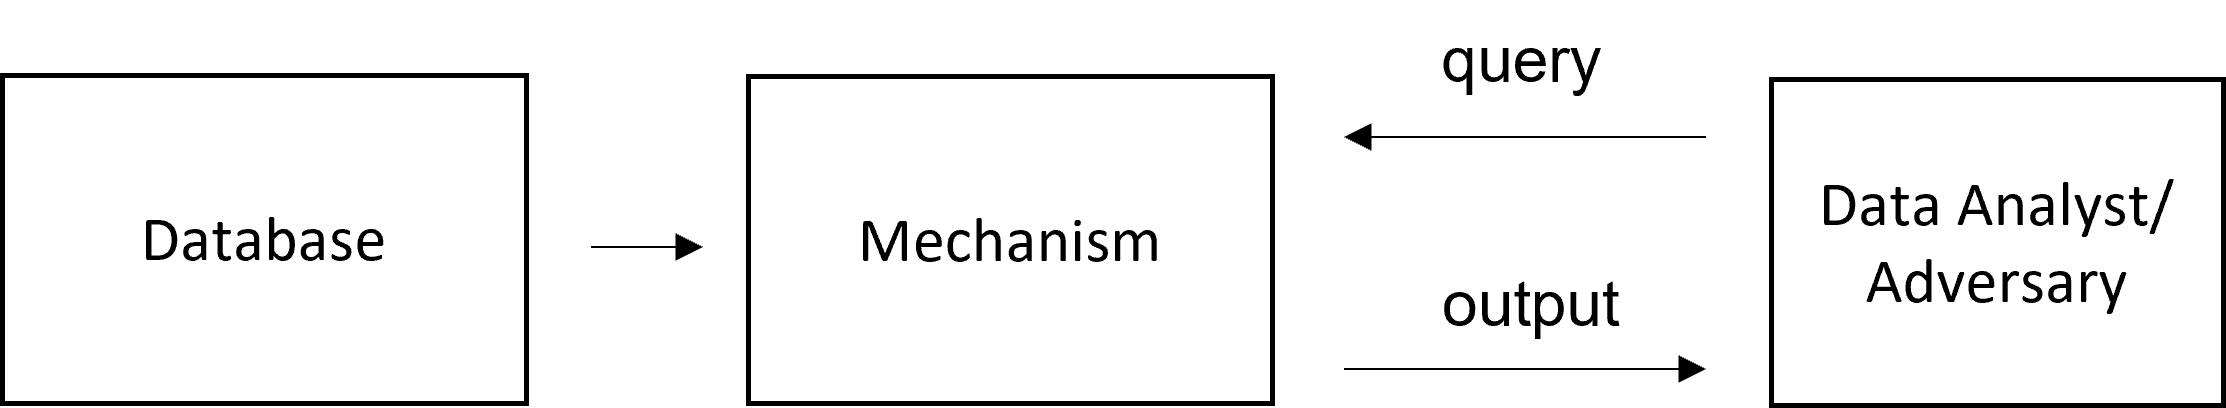
\includegraphics[width=\textwidth]{DP_setting}
    \centering
    \caption{DP setting.}
    \label{img:DPsetting}
\end{figure}
\FloatBarrier
% --------------------------------------------------------------------------

\begin{definition}[Neighboring Databases~\cite{dwork2014algorithmic}]
    Two databases $D_{0}$, $D_{1}\in \mathcal{X}^{n}$  are called neighboring if they differ in exact one entry. This is expressed as $D_{0}\sim D_{1}$.
\end{definition}

\begin{definition}[Differential Privacy~\cite{dwork2014algorithmic}]
    A privacy mechanism $M:\mathcal{X}^{n}\times \mathcal{Q}\rightarrow \mathcal{Y}$ is $\left( \varepsilon ,\delta \right)$-differential privacy if for any two neighboring databases $D_{1}$, $D_{1}\in \mathcal{X}^{n}$, and for all $T\subseteq \mathcal{Y}$, we have $\Pr \left[ M\left( D_{0}\right) \in T\right] \leq e^{\varepsilon}\cdot \Pr \left[ M\left( D_{1}\right) \in T\right] +\delta$ ,
    where the randomness is over the choices made by $M$.
    \label{def:DP}
\end{definition}

Roughly, the differential privacy implies that the distribution of $M$'s output for all neighboring databases is similar. $M$ is called $\varepsilon$-DP (or pure DP) when $\delta = 0$, and $\left(\varepsilon,\delta\right)$-DP (or approximate DP) when $\delta \neq 0$.

\begin{definition}[$L_{1}$ norm]
    The $L_{1}$ norm of a vector $\vec{X}=\left(x_1, x_2, \ldots,x_n \right)^{T}$ measures the sum of the magnitudes of the vectors $\vec{X}$ and is denoted by $\left\|\vec{X}\right\|_{1}=\sum ^{n}_{i=1}\left| x_{i}\right| $.
\end{definition}

\begin{definition}[$L_{2}$ norm]
    The $L_{2}$ norm of a vector $\vec{X}=\left(x_1, x_2, \ldots,x_n \right)^{T}$ measures the shortest distance of $\vec{X}$ to origin point and is denoted by $\left\|\vec{X}\right\|_{2}=\sqrt{\sum ^{n}_{i=1}x_{i}^{2}}$.
\end{definition}

\begin{definition}[$\ell_{t}$-sensitivity~\cite{dwork2014algorithmic}]
    The $\ell_{t}$-sensitivity of a query $f : \mathcal{X}^{n} \rightarrow \mathbb{R}^{k}$ is defined as $\Delta ^{\left(f\right)}_{t}=\max _{D_{0},D_{1}} \left\| f\left( D_{0}\right) -f\left( D_{1}\right) \right\| _{t}$, where $D_{0},D_{1}$ are neighboring databases and $t \in \left\{1,2\right\}$.
    \label{def:sensitivity}
\end{definition}
Recall the Differential Privacy Definition \autoref{def:DP} attempts to \textit{blur} the contribution of any individual in the database using the notion of neighboring databases. Therefore, the sensitivity is a natural quantity when considering differential privacy since it calculates the upper bound of how much $f$ can change when modifying a single entry.


\subsubsection{Motivating Example of Differential Privacy}
\label{subsubsec:motivatingexampleDP}
The previous example about randomized response \autoref{subsubsection:randomizedresponse} indicates that we need DP to solve the trade-off problem between learning useful statistics and preserving the individuals' privacy. In other words, the psychologist wants to find the fraction of students who have cheated in the exam while guaranteeing that no students suffer from privacy leakage by participating in the questionnaire.
To illustrate how DP solves such problems, we adapt the example from~\cite{simpleexplanDP}.
Consider a game as \autoref{prot:motivationexampleDP} shows,
\begin{itemize}
    \item A challenger implements a function $M$ that can calculate useful statistical information. An adversary proposes two data sets $D_{0}$ and $D_{1}$ that differ by only one entry and a test set $Q$.
    \item Given $M\left( D_{0}\right) $, $M\left( D_{1}\right) $ in a random order, the adversary aims to differentiate $D_{0}$ and $D_{1}$. If the adversary succeeds, privacy is violated.
    \item The challenger's goal is to choose $M$ such that $M\left( D_{0}\right) $ and $M\left( D_{1}\right) $ \textit{look} \textit{similar} to prevent them from being distinguished by the adversary.
    \item $M$ is called $\varepsilon$-differentially private iff: $\left| \frac{\Pr \left[ M\left( D_{0}\right) \in Q\right] }{\Pr \left[ M\left( D_{1}\right) \in Q \right] }\right|\leq e^{\varepsilon}$.
\end{itemize}

\begin{protocol}[tbh!]
    \centering
    \fbox{\pseudocode[space=none, syntaxhighlight=auto, addkeywords={input, output}]{%
    \textbf{Challenger $C$} \< \< \textbf{Adversary $A$} \\[0.1\baselineskip][\hline]
    \<\< \\[-0.5\baselineskip]
    \text{input: $M$} \< \< \text{input: $D_0$, $D_1$, $Q$ }\\
    \< \sendmessageleft{top={$D_0$, $D_1$}} \< \<  \\
    \text{$b \sample \bin$} \< \< \\
    \text{$M\left(D_{b}\right)$, $M\left(D_{1-b}\right)$} \< \< \\
    \< \sendmessageright{top={$M\left(D_{b}\right)$, $M\left(D_{1-b}\right)$}} \< \<  \\
    \< \< \text{$b^{\prime}=0$, if $M\left(D_{1-b}\right) \in Q $} \\
    \< \< \text{$b^{\prime}=1$, otherwise} \\
    \< \< \text{if $b==b^{\prime}$, $A$ wins.}
    }}
    \caption{A motivating example of differential privacy.}
    \label{prot:motivationexampleDP}
\end{protocol}
\FloatBarrier

Suppose the adversary $A$ has chosen two data sets:
\begin{itemize}
    \item $D_{0}=\left\{ 0, 0, 0,\ldots ,0\right\} $ ($100$ zeros)
    \item $D_{1}=\left\{ 1, 0, 0,\ldots ,0\right\} $ ($0$ one and $99$ zeroes).
\end{itemize}

The testing set $Q$ is an interval $\left[ T,1\right] $, where the threshold $T$ is chosen by the adversary. The threshold $T$ is chosen such that when the adversary has $T<M\left( D\right) < 1$, he knows $M$ has input $D=D_{1}$ (or $D=D_{0}$, when $0<M\left( S\right) \leq T$) .

\textbf{The Deterministic Case.}
Suppose the challenger wants to calculate the mean value of data sets and chooses $M\left( D\right) =mean\left( D \right) $. Since $M\left( D_{0}\right) =0$ and $M\left( D_{1}\right) =0.01$, the adversary can set $Q =\left[ 0.005,1\right] $ and identify precisely the database $D$ used in $M\left( D\right) $ every time they play the game. In \autoref{img:DPexamplenoisefree}, the blue line represents the distribution of $M\left( D_{0}\right)$, whereas the orange line represents the distribution of $M\left( D_{1}\right)$ (plotted upside down for clarity). The vertical dotted line represents the threshold $T=0.005$ which separates $D_{0}$ and $D_{1}$ perfectly.

\begin{figure}[htbp]
    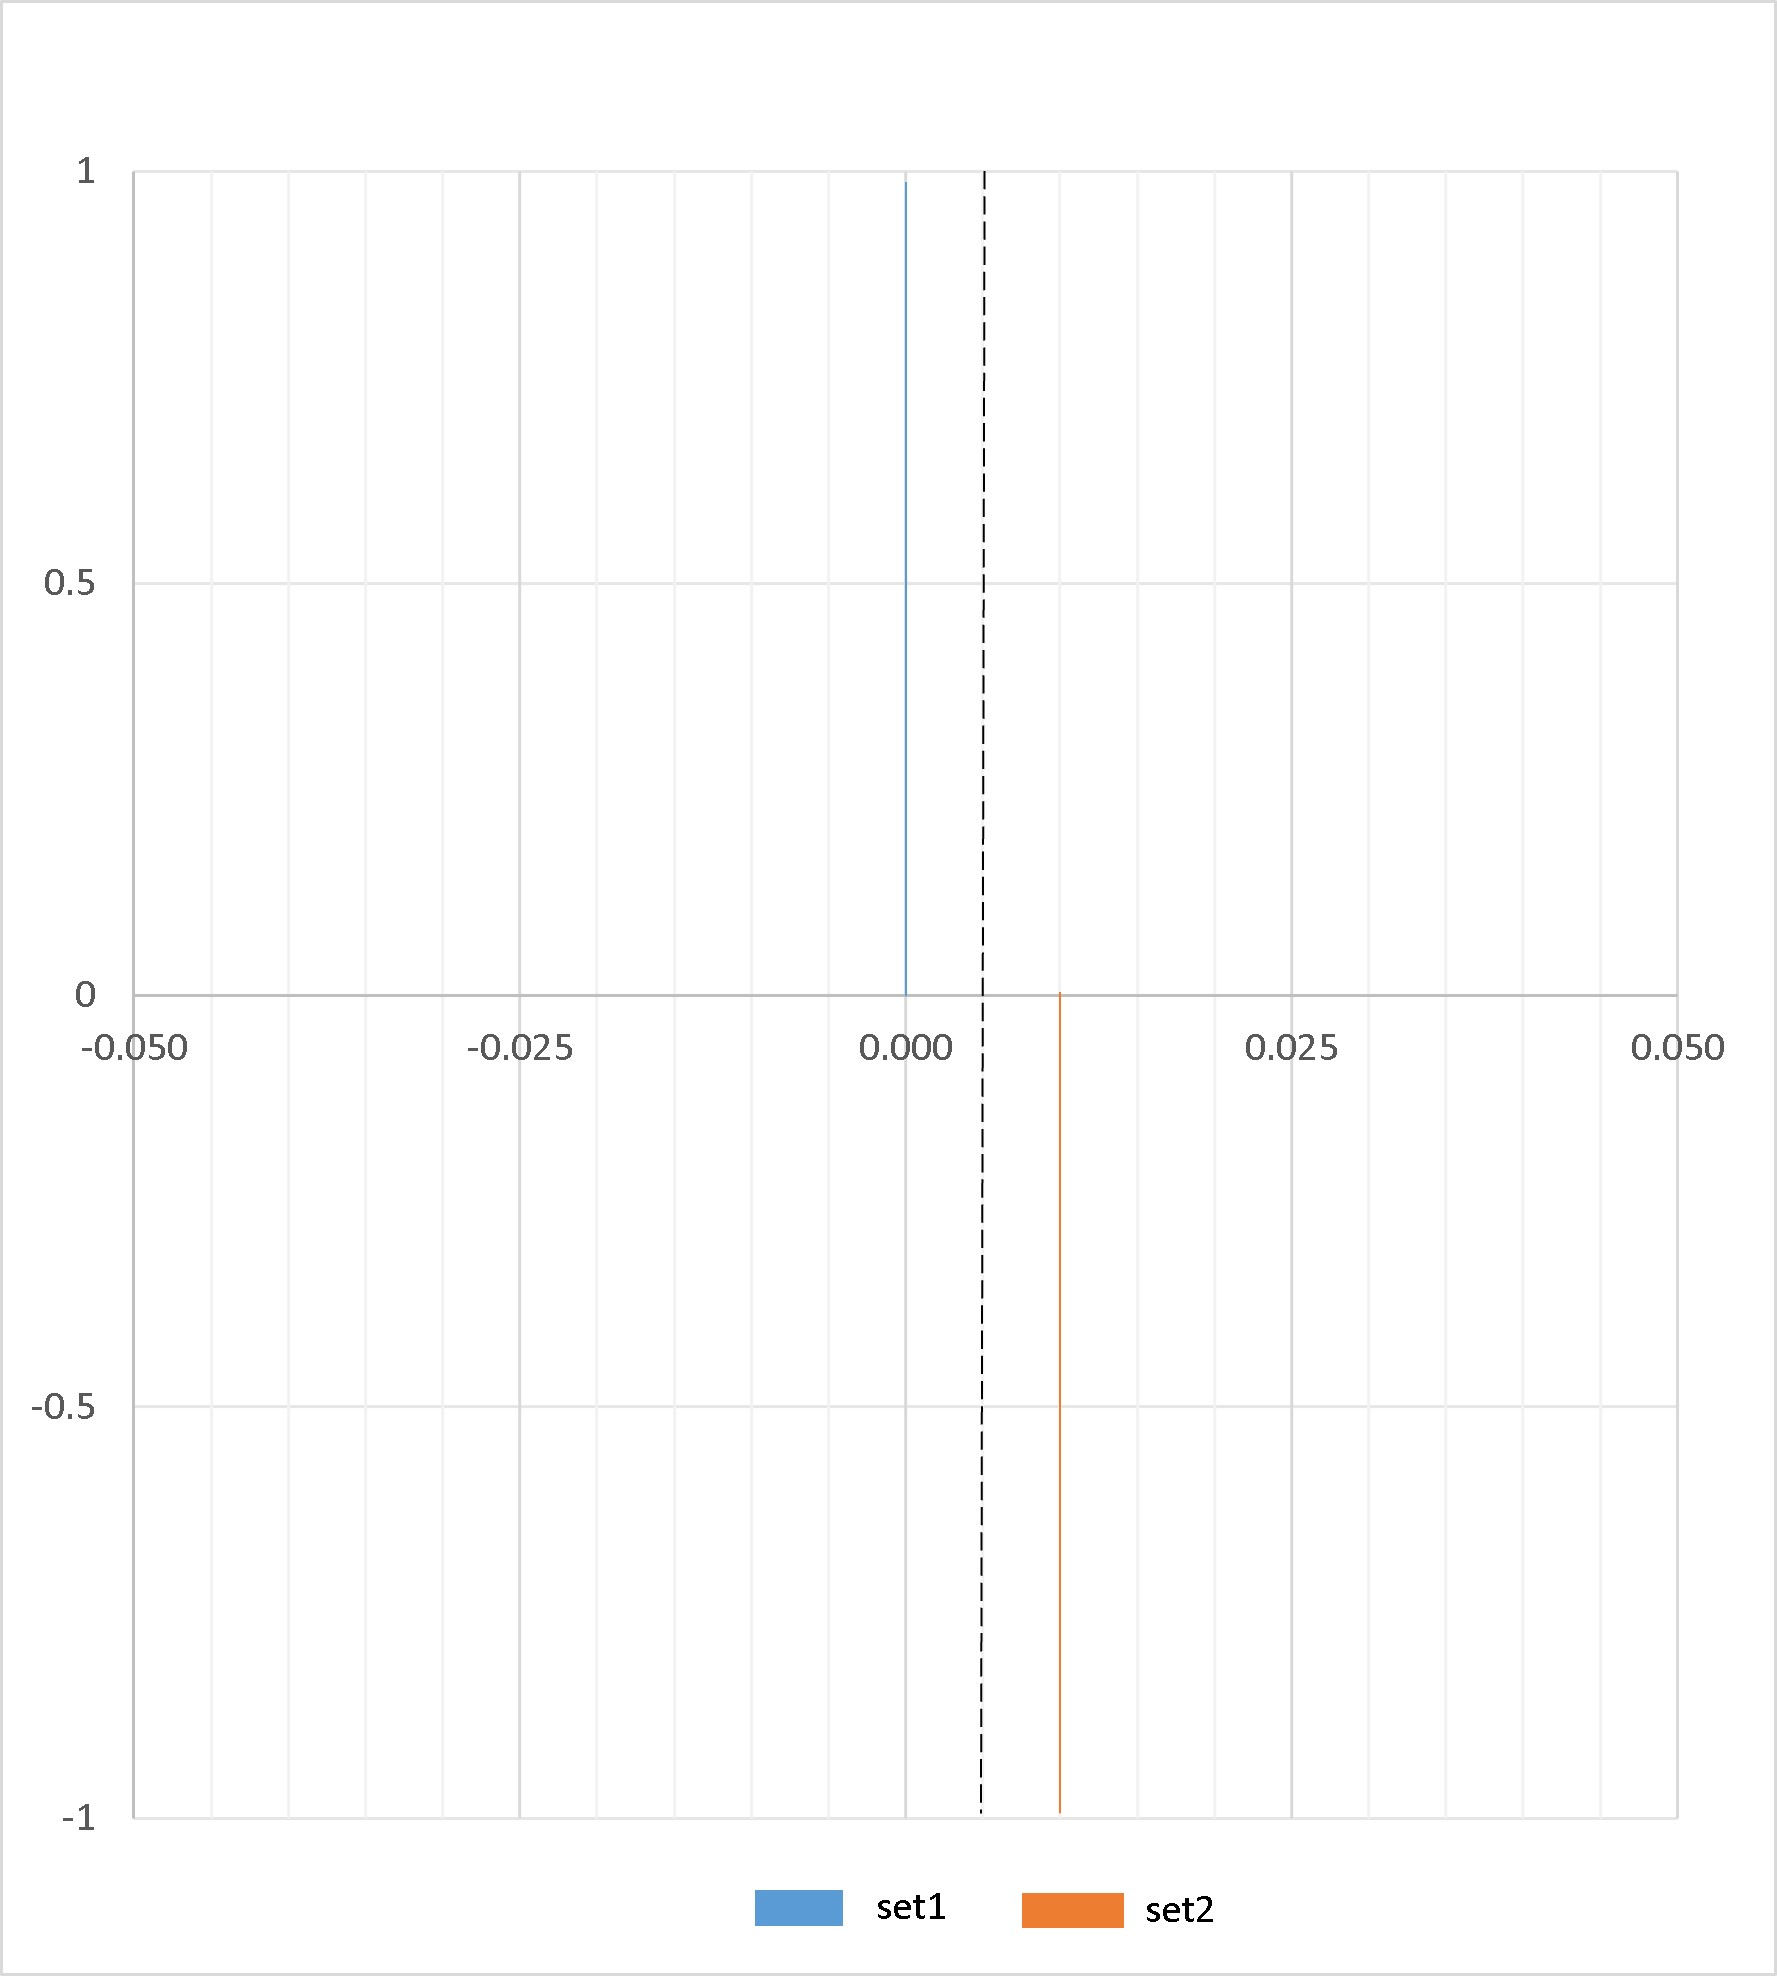
\includegraphics[width=10cm]{DPexamplenoisefree}
    \centering
    \caption{Deterministic algorithm.}
    \label{img:DPexamplenoisefree}
\end{figure}
\FloatBarrier

\textbf{The Indeterministic Case.}
The challenger needs to take some measures to \textit{blur} the difference between $M\left( D_{0}\right)$ and $M\left( D_{1}\right)$. Suppose the challenger decides to add Laplace noise $lap\sim Laplace\left(b=0.05\right)$ to the result of $M\left(D\right)$ as \autoref{img:DPexamplesmallnoise} shows. The shaded blue region is the chance that $M\left( D_{0}\right)$ would return a value greater than the adversary's threshold $T$. In other words, the probability that the adversary would mistake $D_{0}$ for $D_{1}$. In contrast, the shaded orange area is the probability that the adversary identify $D$ as $D_{1}$. The challenger can decrease the adversary's probability of winning by adding more noise as \autoref{img:DPexamplelargenoise} shows, where the shaded blue and orange areas are almost of the same size. Comparing $M\left( D\right)$ with $T$ is no longer reliable to distinguish $D_{0}$ and $D_{1}$. In fact, we have
$\varepsilon=\log \left( \frac{\text{blue area}}{\text{orange area}}\right) $, where $\varepsilon$ expresses the degree of differential privacy and a smaller $\varepsilon$ guarantees a stronger privacy protection. Although the challenger can add more noise to decrease the adversary's success probability, the mean estimation accuracy is also decreased.


\TODO{need reproduce following figures}
\begin{figure}[htbp]
    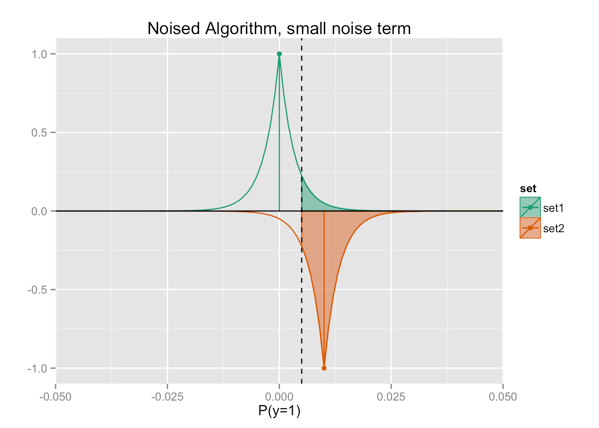
\includegraphics[width=10cm]{DPexamplesmallnoise}
    \centering
    \caption{Indeterministic algorithm with small noise ($b=0.005$).}
    \label{img:DPexamplesmallnoise}
\end{figure}
\FloatBarrier

\begin{figure}[htbp]
    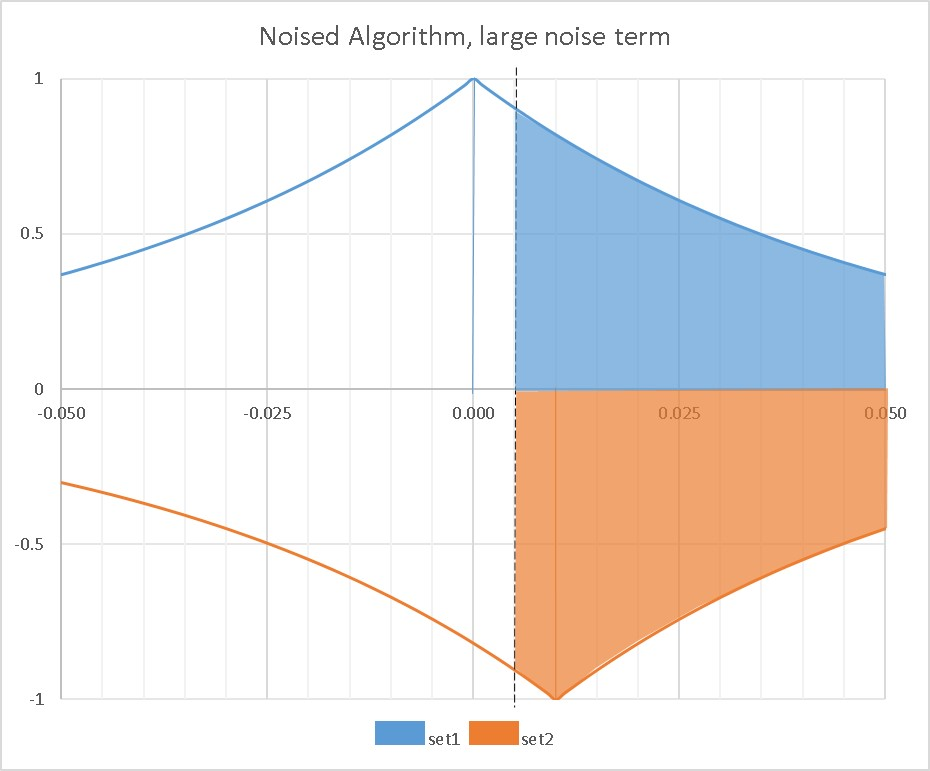
\includegraphics[width=10cm]{DPexamplelargenoise}
    \centering
    \caption{Indeterministic algorithm with large noise ($b=0.05$).}
    \label{img:DPexamplelargenoise}
\end{figure}
\FloatBarrier

\subsubsection{Properties of Differential Privacy}
% One reason for the success of differential privacy is its convenient properties which make it possible to deploy differentially private mechanisms in a modular fashion.

\paragraph{Post-Processing}
\begin{theorem} Let $M:\mathcal{X}^{n} \rightarrow \mathcal{Y}$ be $\left( \varepsilon ,\delta \right)$-DP mechanism, and let $F:\mathcal{Y}\rightarrow \mathcal{Z}$  be an arbitrary randomized mapping. Then $F\circ M$ is $\left( \varepsilon ,\delta=0 \right)$-DP~\cite{dwork2014algorithmic}.
\end{theorem}
The Post-Porcessing properties implies the fact that once a database is privatized, it is still differentially private after further processing.

\paragraph{Group Privacy}
\begin{theorem} Let $M:\mathcal{X}^{n} \rightarrow \mathcal{Y}$ be $\left( \varepsilon ,\delta \right)$-DP mechanism. For all $T\subseteq \mathcal{Y}$, we have $\Pr \left[ M\left(D_{0}\right) +T\right] \leq e^{k \varepsilon}\cdot \Pr \left[ M\left( D_{1}\right) \in T\right] +\delta$, where $D_{0}$, $D_{1}\in \mathcal{X}^{n}$ are two databases that differ in exactly $k$ entries~\cite{dwork2014algorithmic}.
\end{theorem}

Differential privacy can also be defined when considering two databases with more than one entry differences. The larger privacy decay rate $e^{k\varepsilon}$ implies a smaller $\varepsilon$, where \textit{more} noise are necessary to guarantee the same level of privacy.

\paragraph{Basic Composition}
\begin{theorem}
    Suppose $M=\left( M_{1}\ldots M_{k}\right)$  is a sequence of $\left( \varepsilon_{i} ,\delta_{i} \right)$-differentially private mechanisms, where $M_{i}$ is chosen sequentially and adaptively. Then $M$ is $\left(\sum_{i=1}^n\varepsilon_{i} ,\sum_{i=1}^n\delta_{i} \right)$-DP~\cite{dwork2014algorithmic}.
\end{theorem}

Basic Composition provides a way to evaluate the overall privacy when $k$ privacy mechanisms are applied on the same dataset and the results are released.

% \subsection{Comparison between Differential Private Mechanisms}
\subsubsection{Differentially Private Mechanisms}
\label{subsubsec:DPMechanisms}

Differential privacy is a formal framework to quantify the trade-off between privacy and the accuracy of query results. In this part, we introduce two common differentially private mechanisms.

\paragraph{$\varepsilon$-Differential Privacy}
\begin{definition}[Laplace Mechanism~\cite{dwork2014algorithmic}]\
    \label{def:laplaceMechanism}
    Let $f : \mathcal{X}^{n} \rightarrow \mathbb{R}^{k}$. The Laplace mechanism is defined as $M_{Lap}\left( X\right) =f\left( X\right) +\left( Y_{1},\ldots ,Y_{k}\right) $, where the $Y_{i}$ are independent Laplace random variables drawn from a Laplace distribution $Lap \left(  Y_{i}\,|\, b\right) =\frac{1}{2b}e^{\left( -\frac{\left  | Y_{i}\right|}{b}\right)} $ with $b=\frac{\Delta _{1}^{\left(f\right)}}{\varepsilon }$.
\end{definition}

\begin{theorem}
    Laplace Mechanism preservers $\varepsilon$-DP~\cite{dwork2014algorithmic}.
\end{theorem}



% \begin{proof}
%     Let $D_{0}$ and $D_{1}$ be any two neighbouring databases that differs in one entry. Let $\Pr_{D_{0}}\left(z\right) $ and $\Pr_{D_{1}}\left( z\right) $ be the probability density functions of $M\left( D_{0}\right) $ and $M\left( D_{1}\right) $ evaluated at a point $z \in \mathbb{R}^{k}$. To prove differential privacy, it necessary to show that the ratio $\frac{\Pr_{D_{0}}\left( z\right) }{\Pr_{D_{1}}\left( z\right) }$ is bounded by $\varepsilon$, for any arbitrary $z$ and neighboring $D_{0}$ and $D_{1}$ .

%     \begin{align*}
%         \frac{\Pr_{D_{0}}\left( z\right) }{\Pr_{D_{1}}\left( z\right) } & =\frac{ \prod _{i=1}^{k}\exp{\left( -\frac{ \varepsilon \left| f\left( D_{0}\right) _{i}-z_{i} \right|}{\Delta }\right) }}{\prod_{i=1}^{k}\exp{\left( -\frac{ \varepsilon \left| f\left( D_{1}\right) _{i}-z_{i} \right|}{\Delta }\right) } } \\
%                                                                         & =\prod_{i=1}^{k} \exp \left(-\frac{\varepsilon\left(\left|f(D_{0})_{i}-z_{i}\right|-\left|f(D_{1})_{i}-z_{i}\right|\right)}{\Delta}\right)                                                                                                    \\
%                                                                         & \leq \prod_{i=1}^{k} \exp \left(\frac{\varepsilon\left|f(D_{1})_{i}-f(D_{0})_{i}\right|}{\Delta}\right)                                                                                                                                       \\
%                                                                         & =\exp \left(\frac{\varepsilon \sum_{i=1}^{k}\left|f(D_{1})_{i}-f(D_{0})_{i}\right|}{\Delta}\right)                                                                                                                                            \\
%                                                                         & =\exp \left(\frac{\varepsilon\|f(D_{1})-f(D_{0})\|_{1}}{\Delta}\right)                                                                                                                                                                        \\
%                                                                         & \leq \exp (\varepsilon).                                                                                                                                                                                                                      \\
%     \end{align*}
% \end{proof}

% \begin{definition}[Privacy Loss~\cite{dwork2014algorithmic}]
%     Let $X$ and $Y$ be two random variables. The privacy loss random variable  $\mathcal{L}_{X||Y}$ is distributed by drawing $t \sim Y$ , and outputting $\ln ( \frac {\Pr \left[ X=t\right] )}{\Pr \left[ Y=t\right] )} $.
% \end{definition}

% The definition of \emph{Privacy Loss} relies on the assumption that the supports of $X$ and $Y$ are equal, where $supp\left(f\right)=\left\{x \in X: f\left(x\right) \neq 0\right\}$. Otherwise, the privacy loss is undefined since $\Pr\left\{Y=t\right\}=0$.

% From the definition of $\varepsilon$-DP, it is not difficult to see that $\varepsilon$-DP corresponds to $\left|\mathcal{L}_{D_{0}||D_{1}}\right|$ being bounded by $\varepsilon$ for all neighboring databases $D_{0}$, $D_{1}$. In other words, $\varepsilon$-DP says that the absolute value of the privacy loss random variable is bounded by $\varepsilon$ with probability 1.

\paragraph{$\left(\varepsilon,\delta\right)$-Differential Privacy}
$\varepsilon$-DP has strong privacy requirement which leads to adding too much noise and affecting the accuracy of the queries. We introduce an relaxation of $\varepsilon$-DP, $\left(\varepsilon,\delta\right)$-DP.

\begin{definition}[Gaussian Mechanism~\cite{dwork2014algorithmic}]
    Let $f : \mathcal{X}^{n} \rightarrow \mathbb{R}^{k}$. The Gaussian mechanism is defined as $M\left( X\right) =f\left( X\right) +\left( Y_{1},\ldots ,Y_{k}\right) $, where the $Y_{i}$ are independent Gaussian random variables drawn from distribution $\mathcal{N}  \left(  Y_{i}| \mu ,\sigma ^{2}\right) =\frac{1}{\sigma \sqrt{2\pi }}e^{-\frac{1}{2}\left( \frac{Y_{i}-\mu}{\sigma }\right) ^{2}}$ with  $\mu=0$, $\sigma ^{2}=2\ln \left( \frac{1.25}{\delta }\cdot \left( \frac{ \Delta _{2}^{\left(f\right)}) ^{2}}{\varepsilon ^{2}}\right) \right)$ .
    \label{def:gaussianMechanism}
\end{definition}

Gaussian mechanism is proved to satisfy $\left(\varepsilon,\delta\right)$-DP~\cite{dwork2014algorithmic}.



\subsubsection{Discussion about Differential Privacy}

\paragraph{Local and Central Differential Privacy}
Differential privacy is a definition that can be realized in many ways. Two common modes of DP are centralized differential privacy~\cite{dwork2014algorithmic} and local differential privacy~\cite{dinur2003revealing}.

In centralized DP, all data is stored centrally and managed by a trusted curator before the differentially private mechanism is applied. As \autoref{img:DPcentral} shows, the raw data from clients is first collected in a centralized database, then, the curator applies the privacy mechanism and answers the queries $f\left(x\right)$ with $f^{\prime}\left(x\right)$.
The local DP mode is, as \autoref{img:DPlocal} shows, where the clients first apply a privacy mechanism on their data, and send the perturbed data to the curator.
An advantage of local DP mode is that no trusted central curator is needed since the data is perturbed independently before sending to the curator. However, the disadvantage is that the collected data contains redundant noise and may decrease the utility.

\TODO{reproduce following figures}
\begin{figure}[htbp]
    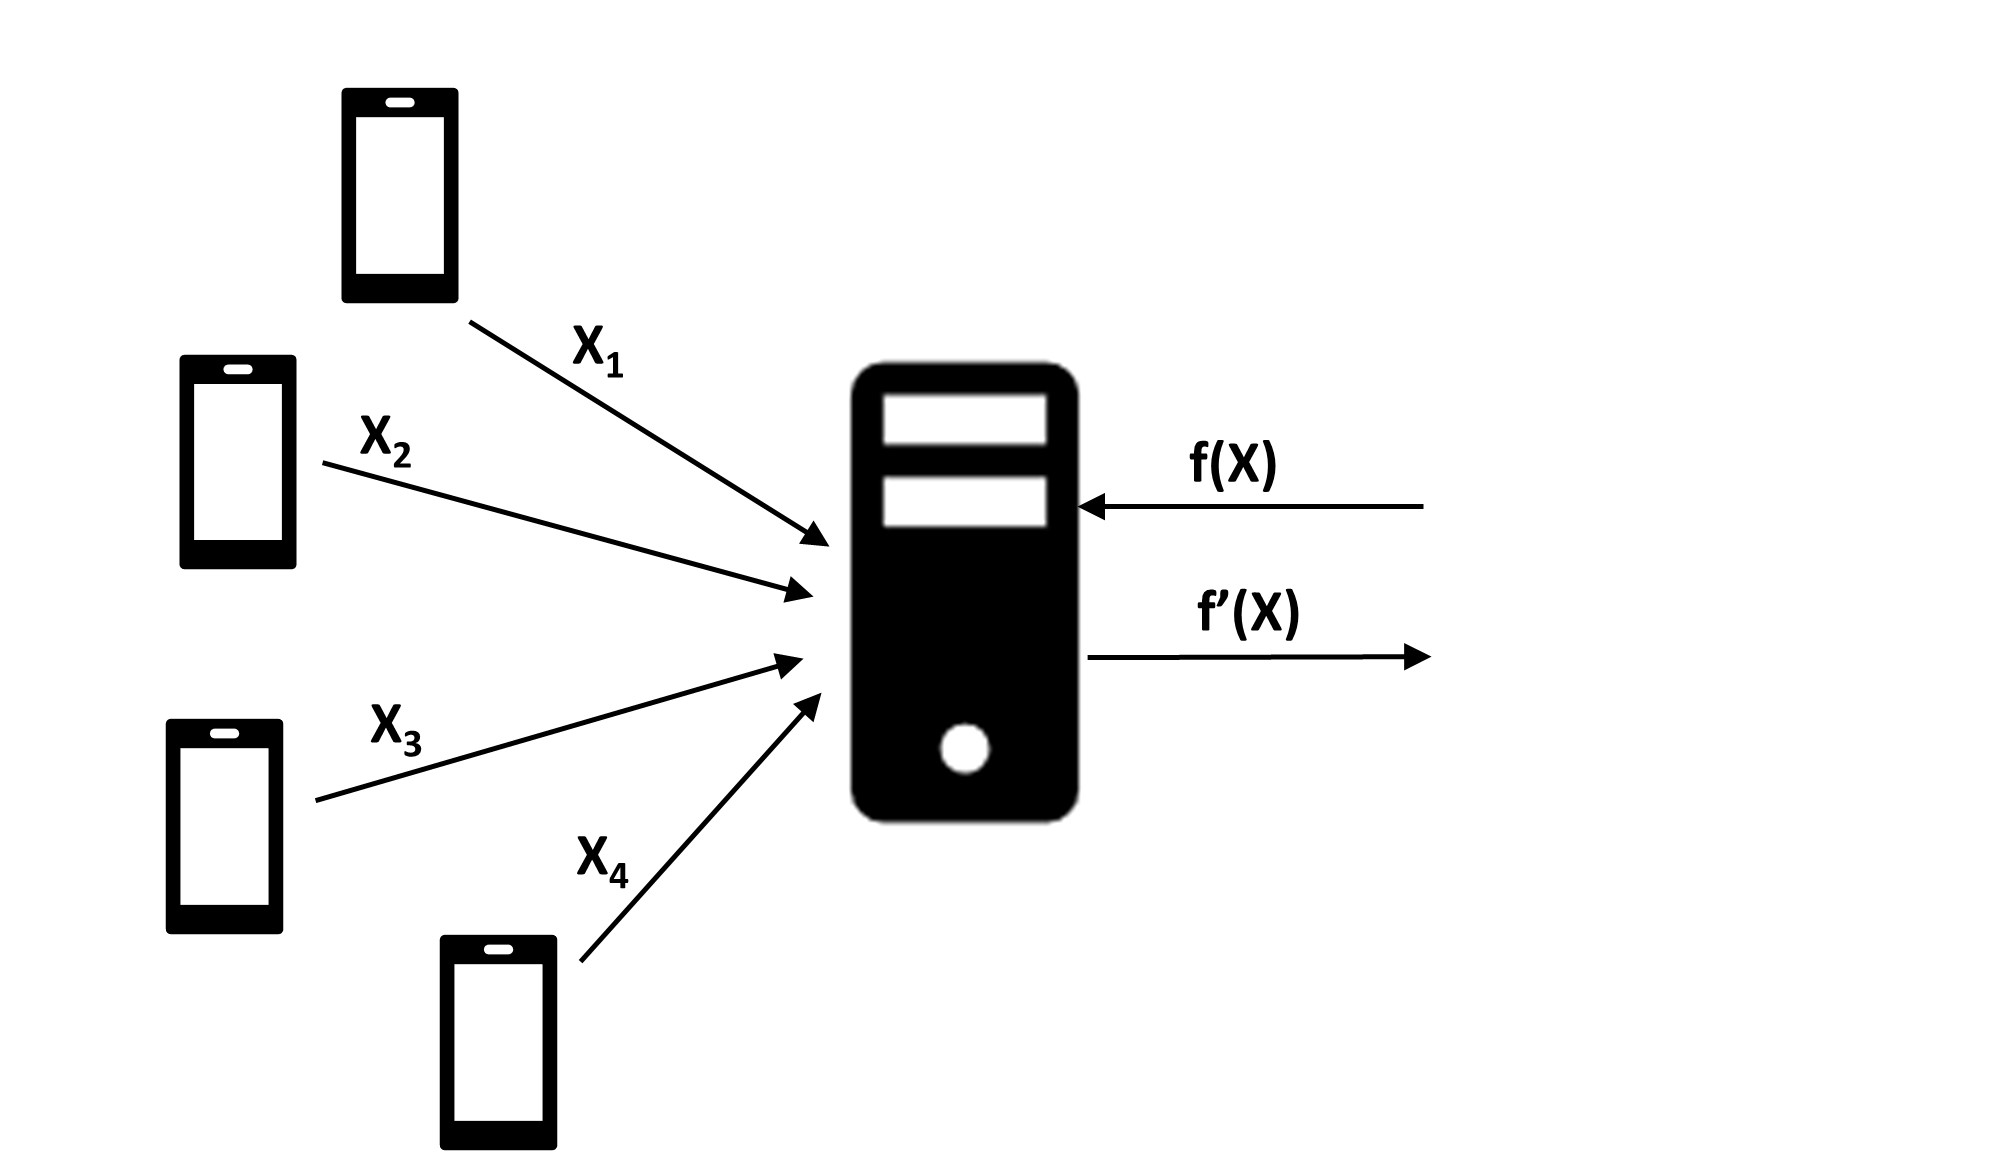
\includegraphics[width=10cm]{DPcentral}
    \centering
    \caption{Centralized DP mode.}
    \label{img:DPcentral}
\end{figure}
\FloatBarrier

\begin{figure}[htbp]
    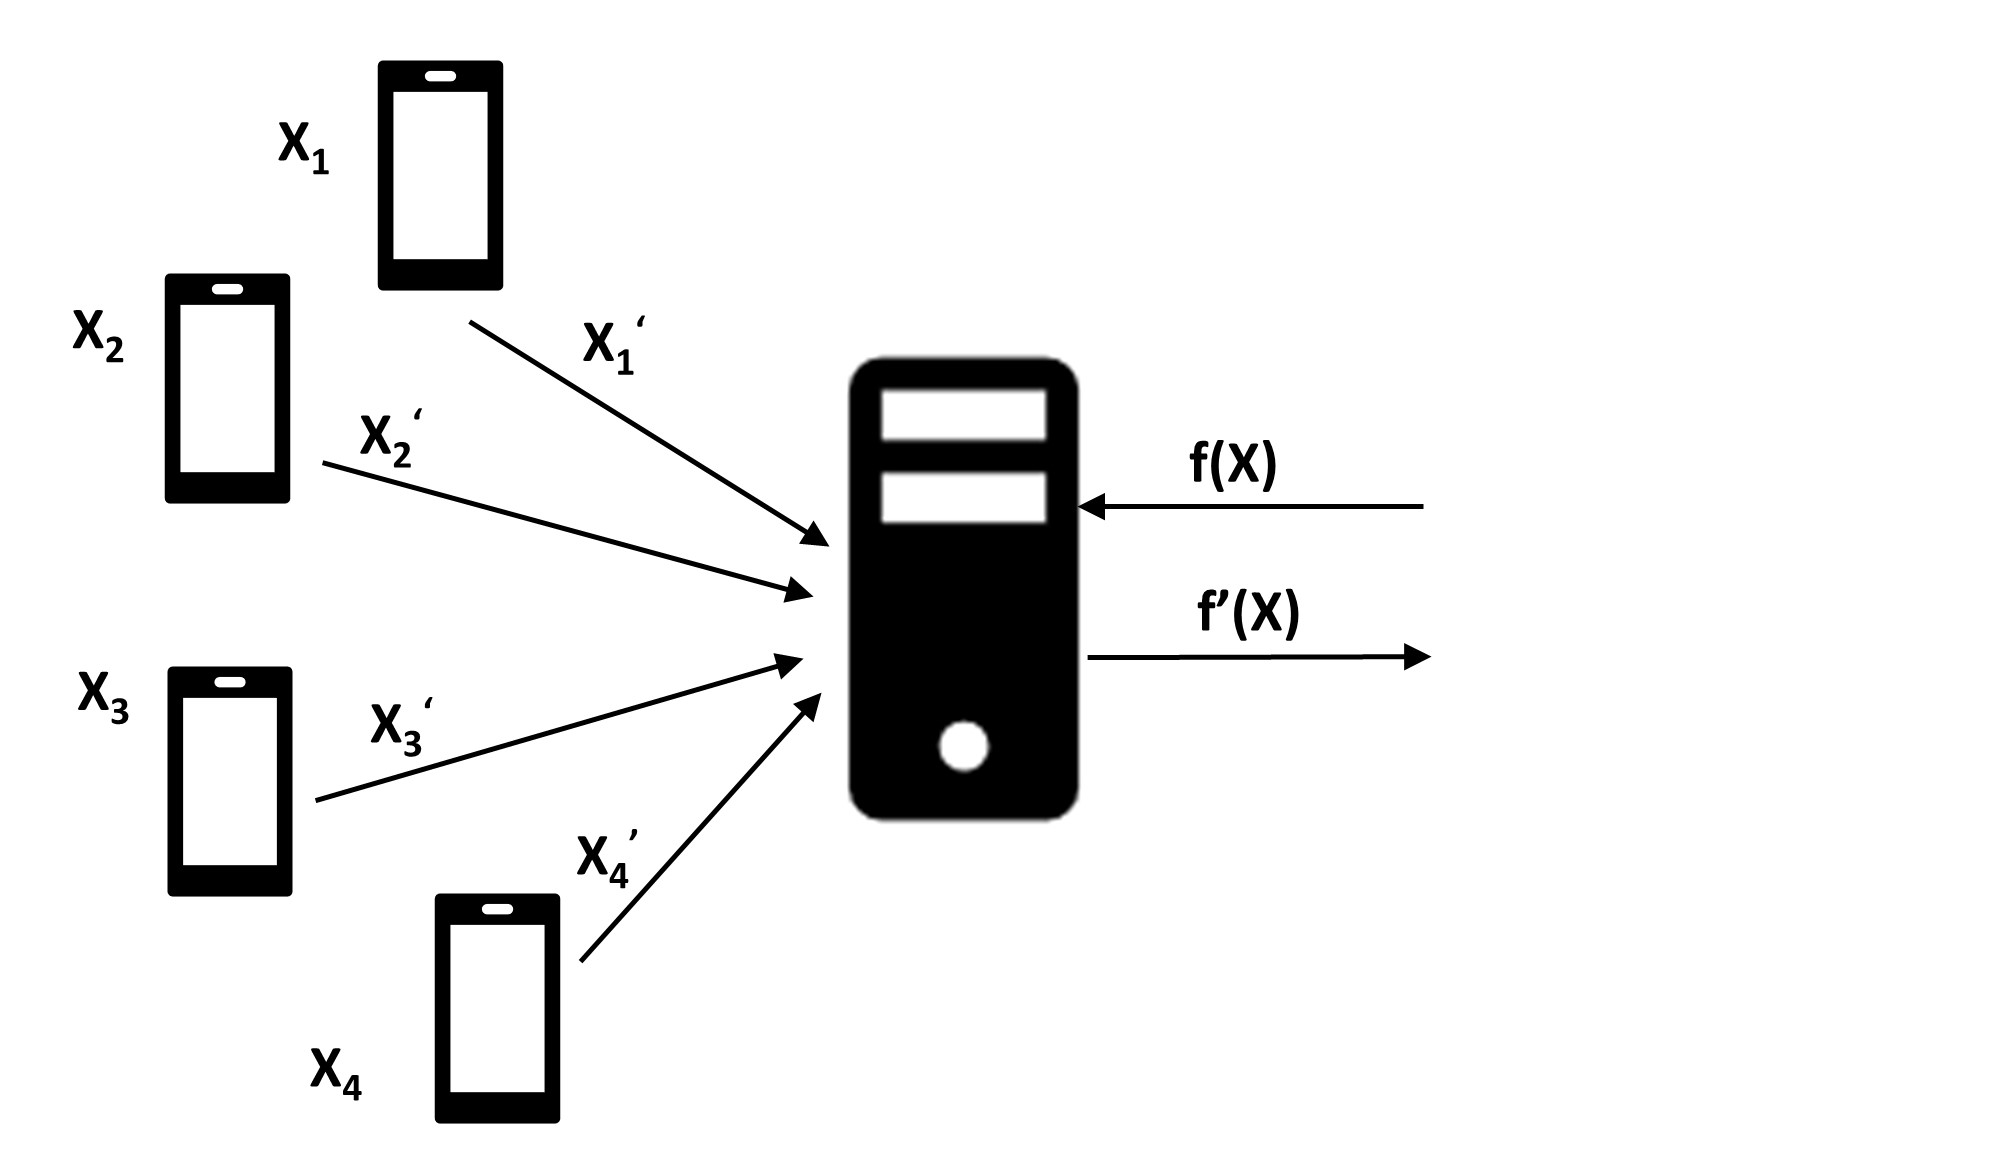
\includegraphics[width=10cm]{DPlocal}
    \centering
    \caption{Local DP mode.}
    \label{img:DPlocal}
\end{figure}
\FloatBarrier


\paragraph{Advantages of Differential Privacy}
From the example \autoref{subsubsec:motivatingexampleDP}, we found that DP can still protect privacy even if the adversary has the knowledge of the database. Generally speaking, DP ensures privacy protection by making no assumption about the adversary's auxiliary information (even when the adversary is the data provider) or computational strategy (regarding the complexity of modern cryptography)~\cite{vadhan2017complexity}. In addition, DP provides a quantitive theory about safely releasing data and maintaining certain level of accuracy.

\paragraph{Challenges of Differential Privacy}
\label{subsubsec:challengesOfDP}
DP provides a method to guarantee and quantify individual privacy at the theoretical level. However, it faces a series of practical challenges.

\textbf{Sensitivity Calculation}. For certain types of data, the sensitivity is not difficult to calculate. Take a database with human ages as an example, the ages should be bounded between $0$ and $150$ (longest human lifespan is $122$ years and $164$ days according to~\cite{whitney_1997}). However, the data with an unbounded value range brings great challenges. A common solution is to roughly estimate the value range and limit the data within that range. For example, if the value range estimation is $\left[ a,b\right] $, then all values smaller than $a$ are replaced by $a$ and all values bigger than $b$ are replaced by $b$. Finally, the sensitivity of query function that outputs ages is ${b- a}$. If value range $\left[ a,b\right] $ is chosen too wide, the utility is potentially destroyed because of the large magnitude of the noise. If the value range $\left[ a,b\right] $ is chosen too narrow, the utility is also potentially decreased because too many values beyond $\left[ a,b\right] $ are truncated.

\textbf{Implementation of DP Mechanisms}. The theory of DP is built upon the real number arithmetic. The practical implementation of differentially private mechanisms relies on floating-point or fixed-point arithmetic only provides an approximation of the mathematical abstractions. Mironov~\cite{mironov2012significance} showed that the irregularities of floating-point implementations and porouse distribution of the Laplace mechanism with textbook sampling algorithm lead to the breach of differential privacy. Further, Gazeau et al.~\cite{gazeau2016preserving} proved that any differentially private mechanism that perturbs data by adding noise with a finite precision can resulting secret disclosure regardless of the actual implementation.

% -------------------------------------------------------------


% Similar to $\varepsilon$-DP, $\left(\varepsilon,\delta\right)$-DP can also be interpreted regarding privacy loss: the absolute value of the privacy loss random variable is bounded by $\varepsilon$ with probability $1 - \delta$~\cite[Lemma 3.17]{dwork2014algorithmic}. In other words, with probability $ \delta$, the privacy of databases is breached.

\chapter{Related Work}
\label{cha:RelatedWork}

\textbf{Combining MPC and DP}
To achieve differential privacy (DP) in a federated learning scenario, either a central trusted server (centralized model) is assumed to perform perturbation to the aggregated result, or each client perturbs its data (decentralized model) before sending it to the central server. However, in the centralized model, the trusted server is responsible for security and privacy and becomes the single point of failure for the entire system. In the decentralized model, when each client perturbs its data to guarantee privacy, the noise in the aggregated result is superfluous and may decrease the utility. 
Several solutions that combine differential privacy and secure multiparty computation (MPC) have been proposed to guarantee privacy and utility. The first key point to solve the problem is deploying MPC instead of the strong assumption of a trusted server. The second point is to reduce redundant noise by ensuring all clients perturbs the data collaboratively rather than independently. 


To the best of our knowledge, \cite{dwork2006our} are the first to consider deploying malicious secure MPC to aggregate and perturb data by generating the noise share of clients in a distributed settings. \cite{dwork2006our} propose methods to generate two types of noise: approximate Gaussian noise with Binomial distribtuion, approximate scaled symmetric exponential (also known as discrete Laplace) distribution with Possion distribution. For Binomial distribution, the protocols requires generating $n$ uniform random bits that would be inefficient for $n\approx 2^{48}$. To discrete Laplace distribution, \cite{dwork2006our} securely evaluating a circuit to generating biased bits, that fails with non-zero probability and requires multiple iterations to make the fail probability negligible. 

\cite{eigner2014differentially} present an architecture called PrivaDA, which combines DP and MPC by generating Laplace and discrete Laplace noise using MPC protocols in a distributed manner. However, the Laplace noise suffers from the attack (\cite{mironov2012significance}) that is caused by the irregularities of floating-point and porous of Laplace distribution. 

(Inherit Differential Privacy in Distributed Setting: Multiparty Randomized Function Computation) propose method for generating Laplace and Gaussian noise in MPC using the central limit theory (intro in preliminary), i.e., the aggregation of a series Bernoulli random variable approximate a normal distribution, $\sqrt{n}\left(\frac{\sum_{i = 1}^{n}  Bern\left(0.5\right) }{n}-\mu\right) \approx \mathcal{N} \left(0,\frac{1}{4}\right)   $. However, the central limit theory only hold when $n \to \infty $, and there is no discussion about how large of $n$ should be taken to guarantee the efficiency of MPC protocols without breaking differential privacy. 

(ref. Efficient Noise Generation to Achieve Differential Privacy with Applications to Secure Multiparty Computation) provide two MPC-based differential privacy protocols for generating shares of finite-range discrete Laplace (FDL) noise and Binomial noise. Contrast to discrete Laplace distribution, which can sample arbitrarily large integers with low probability, FDL can only generate integers in the range . In the FDL noise protocol, each client first locally generates uniform random variable to generate a share of a biased bit and then converts the biased bits shares to discrete Laplace noise, which ensures -differentially privacy. The second protocol for generating Binomial noise also deploys pseudorandom secret-sharing (Cramer et al. 2005) for generating shares of uniform random variables non-interactively and use the Binomial mechanism (Agarwal et al. 2018) but only satisfy computationally -differentially privacy (intro in preliminary).


??? combine floating-point with fixed-point

\textbf{MPC Protocols for Floating-Point Arithmetic}
There are prior works that focus on floating-point arithmetic MPC protocols.  
(ref. Secure Floating-Point Arithmetic and Private Satellite Collision Analysis) provides AGMW based floating-point MPC protocols and using polynomial approximation for $exp$, $sqrt$, etw. 

(ref. Hybrid Model of Fixed and Floating Point Numbers in Secure Multiparty Computations) proposes a hybrid method for AGMW based floating-Point Arithmetic, i.e., representing the mantissa of floating-point as a AGMW based fixed-point and implementing elementary function for it to improved the efficiency of floating-point arithmetic. However, the fixed-point arithmetic is prone to overflow or underflow that requires extra computation check that decrease the overall protocol performance. (ref. Optimizing MPC for Robust and Scalable Integer and Floating-Point Arithmetic) provide optimization for (hybrid model of ....) by parallelizing the polynomial approximation, eliminate branching by representing negative integer using two's complementation, etw. 

(ref. Combining Secret Sharing and Garbled Circuits for Efficient Private IEEE 754 Floating-Point Computations) provides a hybrid protocol for 2-party floating-point arithmetic that convert bgmw sharing to Yao's sharing and evaluate arithmetic operation as Garbled circuits protocols. 



(SecFloat) propose a precise and efficient arithemtic GMW based 32-bit floating-point library for two-party computation. One highlight contribution is the use of mixed-bitwidth computation technique, that use low bitwidth as much as possible. More specifically, for 32-bit floating-point operation, certain operations can be exceuted with $\ell$-bit integers ($\ell <32$), that saves $32-\ell$ bits for computation and communication. One common method to compute function like $log_{2}x$ is polynomial approximation, where high-degree polynomials yields more accurate result but incur more computation. They replace high-degree polynomial with low-degree piecewise polynomial approximiation without decrease accuracy. In other words, for input $x\in \left(a,b\right) $, we evaluate $log_2 x$ using low polynomial by evaluate it in $k$ subintervals ($\left(a, a_1\right) $, $\left(a_1, a_2\right)  $,$\ldots$, $\left(a_{k-1}, b\right) $  ). To determine which subintervals $x$ belongs to, they deploy $LUT$ to map the correct polynomials coefficients. However, we find that SecFloat can't be extended to $N$-party computations ($N\geq 3$) while preserving its efficiency. First, SecFloat relies heavily on the Oblivious Transfer techniques (ref. crytpflow) for mix-bitwidth and $LUT$ operationsm which is not available in multi-party computations. To verify this, we implement the $MSNZB$ (most significant non-zero bit index) protocol deployed in SecFloat using the idea of mix-bitwidth and $LUT$ (ref. fast LUT) in MOTION framework, and compare it with a another implementation of $MSNZB$ that use Boolean GMW operation and share conversion. 

??? table
After the benchmarking, we found that for MPC frameworks that support multiparty computations, the efficiency benefit brought by mix-bitwidth would be negligible as $N$ increases. ??? zero-extension, LUT multiparty complexity analysis. 



(ref. The The Cost of IEEE Arithmetic in Secure Computation) implemente LSSS-based and binary circuit-based floating-point arithmetic MPC protocols and compare their performance. In their benchmarking result, the LSSS-based floating-point operation is about $10-100x$ faster than binary circuit-based floating-point operation. However, in our implementation, the binary circuit-based floating-point operation is $5-10x$ faster than LSSS-based floating-based without SIMD and can be up to $1000x$ faster than LSSS-based floating-point operation when amortized over SIMD=1000.

\textbf{MPC Protocols for Fixed-Point Arithmetic}
(ref. High-precision Secure Computation of Satellite Collision Probabilities) provides methods for 2-party fixed-point arithmetic by combine AGMW and BGMW, i.e., using AGMW for integer addition and multiplication using AGMW and BGMW for integer comparison, shifting, $exp$, etw. 

(ref.  Benchmarking Privacy Preserving Scientific Operations) provides AGMW based fixed-point arithmetic. 

(ref. Round-Efficient Protocols for Secure Multiparty Fixed-Point Arithmetic) agmw fixed-point. 







\chapter{Secure Differentially Private Mechanisms On Finite Computer}
\label{cha:secureDPMechanisms}

Generally, the security analysis of differentially private mechanisms is based on two implicit assumptions: (i) Computations are performed on real numbers and require machines to have infinite precision, (ii) The noise is sampled from a probability distribution that is very close to the theoretically correct probability distribution. However, the practical implementation of differentially private mechanisms is based on floating-point or fixed-point arithmetic that only provides finite order of accuracy. Mironov~\cite{mironov2012significance} showed that the porous distribution of the Laplace random noise sampled with textbook algorithm under floating-point implementaion couild lead to violation of differential privacy. In this chapter, we describe four types of existing differentially private mechanisms~\cite{mironov2012significance,googleDP2019,ghosh2012universally,canonne2020discrete} and modify corresponding sampling algorithms for generating secure noise on the finite computer. We construct MPC protocols for these differentially private mechanisms and sampling algorithms in~\autoref{cha:MPCProtocolsforDifferentiallyPrivateMechanisms}.



% Recall that differentially private mechanisms (cf.~\autoref{subsec:DPMechanisms}) guarantee differential privacy by adding appropriately chosen random noise to a query function $f\left(D\right)  $, which can be expressed as:

% \[M\left(D\right)=f\left(D\right)+Y,\]

% where $D$ is the database, $Y $ is the noise term.




% However, we only have machines with finite-precision for the practical implementations of differentially private mechanisms. We typically use fixed-point or floating-point arithmetic to approximate the operations of real numbers. Mironov~\cite{mironov2012significance} shows that the porous distribution of the Laplace noise implemented with the textbook noise sampling methods under floating-point arithmetic can lead to severe differential privacy breaching and proposes the snapping mechanism to avoid such security issues by rounding and smoothing the output of the Laplace Mechanism (cf.~\autoref{def:laplaceMechanism}). \CHANGED{Google Differential Privacy Team~\cite{googleDP2019} introduces an alternative secure approach that scales integer noise from certain distribution under floating-point arithmetic to approximate continuous noise in desired distribution and yields better accuracy than the snapping mechanism}. \CHANGED{Canonne et al.~\cite{canonne2020discrete} provide algorithms to sample discrete Laplace and Gaussian noise on finite computer for the query function $f\left(D\right) \in \mathbb{Z} $}.


\section{Snapping Mechanism}
\label{sec:snappingMechanism}
Recall that Laplace mechanism (cf.~\autoref{subsubsec:DPMechanisms}) guarantees $\varepsilon$-DP by adding Laplace random variable $Y \sim Lap\left(\lambda\right) $ to the query function $f\left(D\right)  $ with database $D$:
\begin{equation}
    \begin{split}
        M\left(D, \lambda\right)=f\left(D\right)+Y.
    \end{split}
\end{equation}


As discussed in \autoref{algo:InverseTransform-BasedLaplaceSamplingMethod}, we can generated a Laplace random variable $Y$ by transforming the random chosen sign $S\in \left\{-1,1\right\} $ and a uniform random variable $U \in \left(0,1\right] $ (or $U \in \left(0,1\right) $ if we ignore the \textit(small) probability of generating exact $1$) as follows:
\begin{equation}
    \begin{split}
        Y \gets S \cdot \lambda \ln\left(U\right)
    \end{split}
\end{equation}

Mironov~\cite{mironov2012significance} showed that the Laplace random variable $Y$ generated in this method under floating-point arithmetic could lead to severe differential privacy breaching and proposed the snapping mechanism to avoid such security issues by rounding and smoothing the output $f\left(D\right)+Y$ in a specific approach.

% In this section, we describe the snapping mechanism that is immune to the attack
% \CHANGED{Laplace random variable $Y \sim Lap\left(\lambda\right) $ (cf.~\autoref{def:LaplaceDistribution}) can be generated with the inverse transform sampling method (cf.~\autoref{theorem:inversionSamplingMethod}):}
% \begin{equation}
%     \begin{split}
%         % Y&=\left(2Z-1\right)\cdot b \ln\left(1-U\right)\\
%         Y&=S\cdot \lambda \ln\left(U\right),
%     \end{split}
% \end{equation}
% where $S\in \left\{-1,+1\right\} $ is the sign, $\lambda$ controls the magnitude of $Y$, and $U$ is a uniform random variable in the interval $(0,1]$.

% Mironov~\cite{mironov2012significance} demonstrates an attack on the floating-point implementation of the Laplace mechanism (cf.~\autoref{def:laplaceMechanism}) based on the above noise generation method and proposes the snapping mechanism $M_S$ to guarantee differential privacy with rounding and clamping operations, that is defined as:

The snapping mechanism is defined as follows:
\begin{equation}
    \begin{split}
        M_{S}\left(f\left(D\right),\lambda,B\right) =\text{clamp}_{B}\left(\left\lfloor\text {clamp }_{B}\left(f\left(D\right) \right) \oplus S\otimes \lambda\otimes \text{LN}\left(U^{*}\right) \right\rceil_{\Lambda}\right).
    \end{split}
\end{equation}

% \TODO{explain exact rounding}

Let $\mathbb{D}$ denote the set of floating-point numbers, and $\mathbb{D} \cap \left(a,b\right) $ denote all the floating-point numbers in the interval $\left(a,b\right)$.
$f\left(D\right) \in \mathbb{D} $ is the query function of database $D$, and $S\otimes \lambda\otimes \text{LN}\left(U^{*}\right)$ is the noise term.
$S$ is the sign of the noise that is uniformly distributed over $\left\{-1,1\right\} $. $U^{*}$ is a \textit{uniform} distribution over $\mathbb{D} \cap \left(0,1\right) $, and generates floating-point numbers with probability proportional to its \textit{unit in the last palce} (ulp), i.e., spacing between two consecutive floating-point numbers. \CHANGED{$\text{LN}(x )$ is the natural logarithm under floating-point implementation with exact rounding, i.e., $\text{LN}(x )$ rounds input $x$ to the closest floating-point number with probability $p=1$.}
$\oplus$ and $\otimes$ are the floating-point implementations of addition and multiplication.

Function $\text{clamp}_{B}\left(x\right) $ limits the output to the interval $\left[-B, B\right] $ by outputting $B$ if $x > B$, $-B$ if $x < -B$, and $x$ otherwise.   $\Lambda$ is the smallest power of two greater than or equal to $\lambda$, and we have $\Lambda=2^{n}$ such that $2^{n-1} < \lambda \leq2^{n}$ for $n \in \mathbb{Z} $. Function $\lfloor x\rceil_{\Lambda}$ rounds input $x$ exactly to the nearest multiple of $\Lambda$ by manipulating the binary representation of floating-point number $x$.

Note that the snapping mechanism assumes that the \textit{sensitivity} $\Delta_1 ^{\left(f\right) } $ (cf.~\autoref{def:sensitivity}) of query function $f$ is $1$, which can be extended to an arbitrary query function $f^{\prime}$ with \textit{sensitivity} $\Delta _1^{\left(f^{\prime}\right) }\neq 1$ by scaling the output of $f^{\prime}\left(D\right) $ with $f\left(D\right) =\frac{f^{\prime}\left(D\right) }{\Delta_1 ^{\left(f^{\prime}\right) }}$.

\begin{theorem}[{~\cite{mironov2012significance}}]
    The snapping mechanism $M_{S}\left(f\left(D\right),\lambda,B\right)$ satisfies $\left(\frac{1}{\lambda}+\frac{2^{-49}B}{\lambda}\right) $-DP for query function $f$ with \textit{sensitivity} $\Delta _1^{\left(f\right) } =1$ when $\lambda<B<2^{46}\cdot\lambda$.
\end{theorem}
% \TODO{prove about snapping mechanism DP properties and correctness}

% \subsection{Implementations of Snapping Mechanism}
% \label{subsec:snappingImp}

% We introduce snapping mechanism implementations from~\cite{Covington2019} and adapt them into MPC protocols in~\autoref{sec:snappingMPC}, other implementations of snapping mechanism are known as~\cite{George2017, Ristea2021}.

The computation of snapping mechanism consists of the following steps:
\begin{enumerate}
    \label{enu:snappingSteps}
    \item $\text{clamp}_B\left(\cdot\right) $.
    \item Generation of $U^{*}$ and $S$.
    \item Floating-point arithmetic operations such as $\text{LN}\left(\cdot\right) $, $\oplus$, and $\otimes $.
          % \item Calculation of $\Lambda$.
    \item Operation $\lfloor x\rceil_{\Lambda}$ that rounds input $x$ to the nearest multiple of $\Lambda $.
\end{enumerate}
We briefly describe how to generate $U^{*}$. The implementation details of the other steps can be found in the Covington's work~\cite{Covington2019}.


% \subsubsection{Generation of $U^{*}$}
% \label{subsubsec:generationUStar}

\textbf{Generation of $U^{*}\in\mathbb{D} \cap \left(a,b\right)  $.}
$U^{*}$ is a \textit{uniform} distribution over $\mathbb{D} \cap \left(0,1\right) $ and can be represented in IEEE 754 floating-point~\cite{IEEE754_2019} as:
\begin{equation}
    \begin{split}
        U^{*}=\left(1.d_{1}\ldots d_{52}\right)_{2}\times2^{e-1023}.
    \end{split}
\end{equation}

As discussed above, each floating-point $U^{*}$ should be output with a probability proportional to its ulp. We sample a floating-point number from $U^{*}$ using $Algo^{RandFloat1}$~\cite{walker1974fast,mironov2012significance}, i.e., independently sampling a geometric random variable $x \sim Geo\left(0.5\right) $, and the significant bits $\left(d_{1},\ldots ,d_{52}\right)\in\left\{0,1\right\}^{52} $. Then, we set $U^{*}$'s biased exponent $e=1023-\left(x+1\right) $.

\begin{algorithm}[tbh!]
    \centering
    \fbox{
    \pseudocode[space=none, syntaxhighlight=auto, addkeywords={Algorithm, Input, Output, IF,TO,RETURN, FOR, ELSE IF, ELSE, WHILE},linenumbering, skipfirstln, head=\textbf{Algorithm: $Algo^{RandFloat1}$}]{
    \textbf{Input: None} \pcskipln \\
    \textbf{Output: $U^{*}\in \mathbb{D} \cap \left(0,1\right)$} \\
    \text{$\left(d_1,\ldots,d_{52}\right)\sample \left\{0,1\right\}^{52} $}\\
    \text{$x \gets Algo^{Geo}\left(0.5\right)  $}\\
    \text{$e \gets 1023-\left(x+1\right) $}\\
    \text{RETURN $U^{*}=\left(1.d_1\ldots d_{52}\right)_2 \times 2^{e-1023}$}
    }}
    \caption{Algorithm for sampling uniform random floating-point number $U^{*}\in\mathbb{D} \cap \left(a,b\right) $.}
    \label{algo:RandFloat1}
\end{algorithm}
\FloatBarrier

As $U^{*}$'s significant bits are sampled randomly from $\left\{0,1\right\}^{52} $, the floating-point numbers with identical biased exponent $e-1023$ are distributed uniformly in $U^{*}$.
Further, $x \sim Geo\left(0.5\right) $ guarantees that the probability of sampling a floating-point number from $U^{*}$ is proportional to its ulp.
Intuitively, \textit{uniformly} sampling a floating-point number can be thought of as randomly drawing a real number in the interval $\left(0,1\right) $ and rounding it to the nearest floating-point number. However, the floating-point numbers are discrete and not equidistant. For example, there are exactly $2^{52}$ representable reals in the interval $[.5, 1)$ and $2^{52}$ reals in the interval $[ .25, .5)$. If we only sample the floating-point numbers with equal distance to each other in the interval $\left(0,1\right) $, a large amount of floating-point numbers would be ignored. As discussed in~\cite{walker1974fast,mironov2012significance}, a better approach is to sample floating-point numbers with probability proportional to its ulp (i.e., spacing to its consecutive neighbor).
With $x\sim Geo\left(0.5\right) $, the total sampling probability for the floating-point numbers in the interval $(0,1)$ with exponent $e-1023=-\left(x+1\right) =-1$ is $Pr\left(x=0 \,|\,0.5\right) =\frac{1}{2}$.
The total sampling probability for the floating-point numbers in the interval $(0,0.5)$ with exponent $e-1023=-2$ is $Pr\left(x=1\,|\,0.5\right) =\frac{1}{2^2}$ , etc.
Therefore, we have a total sampling probability for the floating-point numbers in in the interval $\left(0,1\right)$ is $\sum_{i = 1}^{\infty}\frac{1}{2^{i}}\approx 1$.


% % \TODO{image about uniform sampling of floating point number}
% \autoref{img::floatingpointdistribution} shows the distribution of floating-point numbers (in form $\left(-1\right)^S\left(1.d_{1}d_{2}d_{3} d_{4}\right)_2\times 2^{\left(e_{1}e_{2} e_{3}\right)_2-3}$) in the interval $\left(-2,2\right) $, where each vertical line represents a floating-point number. Suppose there are $2t$ floating-point numbers in the interval $\left(0,0.5\right) $ with distance $d$ to each other, and $t$ floating-point numbers in the interval $\left(0.5,1\right) $ with distance $2d$, and in total $3t$ floating-point numbers in the interval $\left(0,1\right) $. 
% With the above sampling methods \autoref{algo:RandFloat1}, $t$ floating-point numbers in the interval $\left(0,0.5\right) $ (with distance $2d$ to each other) and $t$ floating-point numbers in the interval $\left(0.5,1\right) $ (with distance $2d$ to each other) have the same probability (total probability $p=0.5$), the rest floating-point numbers in the interval $\left(0,0.5\right) $ would be sampled with total probability $p=0.25$. Finally, each floating-point number in the interval $\left(0,1\right) $ would be sampled with the same probability $p=\frac{0.25}{a}$. 

% \begin{figure}[htbp]
%     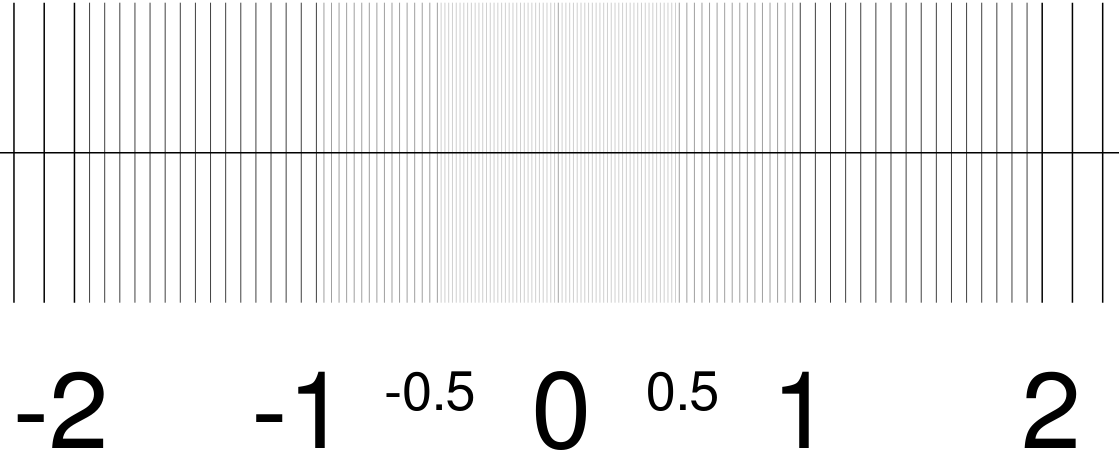
\includegraphics[width=\textwidth]{floating_point_distribution}
%     \centering
%     \caption{Floating point $\left(-1\right)^S\left(1.d_{1}d_{2}d_{3} d_{4}\right)_2\times 2^{\left(e_{1}e_{2} e_{3}\right)_2-3}$ distribution.}
%     \label{img:floatingpointdistribution}
% \end{figure}
% \FloatBarrier

% \subsubsection{Calculation of $\Lambda$}
% \label{subsubsec:calLambda}
% The snapping mechanism uses input $\lambda$ to calculate $\Lambda$. For $n \in \mathbb{Z} $, $\Lambda=2^{n}$ is the smallest power of two greater than or equal to $\lambda$, i.e., $2^{n-1} < \lambda \leq 2^{n}$.

% We can represent $\lambda$ in IEEE 754 floating-point (cf.~\autoref{subsubsec:floatingPoint}) as follows:

% \[ \lambda = (-1)^0 \left(1.d_{1} \hdots d_{52}\right)_2 \times 2^{\left(e_1 \hdots e_{11}\right)_2-1023}. \]

% The calculation of $\Lambda$ can be divided into two cases: (1) $\lambda=2^{n}$ for $n \in \mathbb{Z} $, which requires $\left(d_i\right)_{i \in \left[52\right]} = 0$; (2) $2^{n-1}<\lambda<2^{n}$ for $n \in \mathbb{Z} $. For the first case, we can get $\Lambda\gets \lambda$ since $\lambda=2^{n}$ is already a power of two. For the second case, we can calculate $\Lambda$ by increasing the exponent of $\lambda$ by $1$ and setting all its significant bits $\left(d_i\right)_{i \in \left[52\right]} $ to $0$.

% In summary we have

% \begin{equation}
%     \Lambda =
%     \begin{cases}
%         \lambda                                                                           & \text{ if for } i \in \left[52\right] \text{, } \forall i: d_i = 0    \\
%         \left(1.\overline{0}\right)_2 \times 2^{\left(e_1 \hdots e_{11}\right) _2-1023+1} & \text{ if for } i \in \left[52\right] \text{, } \exists i: d_i \neq 0
%     \end{cases}
% \end{equation}

% \subsubsection{Rounding $x$ to the nearest multiple of $\Lambda=2^n$}
% \label{subsubsec:roundX2Lambda}

% We represent $x$ in IEEE 754 floating-point (cf.~\autoref{subsubsec:floatingPoint}) as follows:
% \[ x = \left(-1\right)^S \left(1.d_{1} \hdots d_{52}\right)_2 \times 2^{\left(e_1 \hdots e_{11}\right)_2-1023}. \]

% $\lfloor x \rceil_{\Lambda}$ is done in three steps:
% \begin{enumerate}
%     \item $x^{\prime} = \frac{x}{\Lambda}=x\cdot 2^{-n}$,
%     \item $x^{\prime\prime}=\left\lfloor x^{\prime}\right\rceil $,
%     \item $\lfloor x \rceil_{\Lambda} = x^{\prime\prime} \cdot   \Lambda  =x\cdot 2^{n}$,
% \end{enumerate}
% where $\left\lfloor \cdot \right\rceil$ rounds the input to the nearest integer.
% % \paragraph{1. $x^{\prime} = \frac{x}{\Lambda}$}

% % We represent $x$ in IEEE 754 floating-point (cf.~\autoref{subsubsec:floatingPoint}) as follows:
% % \[ x = \left(-1\right)^S \left(1.d_{1} \hdots d_{52}\right)_2 \times 2^{\left(e_1 \hdots e_{11}\right)_2-1023}. \]
% % Since $\Lambda=2^n$ is a power of two, the division $\frac{x}{\Lambda}$ can be performed by substracting $n$ from the exponent of $x$ and we get:
% % \[ x^{\prime} = \left(-1\right)^S \left(1.d_{1} \hdots d_{52}\right)_2 \times 2^{\left(e_1 \hdots e_{11}\right)_2-1023-n}. \]

% The first step ($x^{\prime} = \frac{x}{\Lambda}$) and last step ($\lfloor x \rceil_{\Lambda} =   x^{\prime\prime} \cdot \Lambda $) are calculated by manipulating (substraction or addition) the exponent of $x$ and $x^{\prime\prime}$. Note that one exception is when $x=0$ or $x^{\prime\prime}=0$, because for floating-point number $0=\left(-1\right) ^0 (1.\overline{0})_2\times 2^{\left(0000000000\right)_2-1023 }$, $0\times 2^n\neq \left(-1\right) ^0 (1.\overline{0})_2\times 2^{\left(0000000000\right)_2-1023+n }$ as discussed in~\cite{IEEE754_2019}.

% \paragraph{Calculate $x^{\prime\prime}=\left\lfloor x^{\prime}\right\rceil $ }
% \label{para:roundX2Int}

% Suppose $x^{\prime} = \left(-1\right)^S \left(1.d_{1} \hdots d_{52}\right)_2 \times 2^{\left(e_1 \hdots e_{11}\right)_2-1023-n}$. Let $y=\left(e_1 \hdots e_{11}\right)_2-1023-n$, and we have
% \[ x^{\prime} = \left(-1\right)^S \left(1.d_{1} \hdots d_{52}\right)_2 \times 2^{y}.\]
% The calculation of $x^{\prime\prime}=\left\lfloor x^{\prime}\right\rceil $ is categorized in five cases depending on the value of unbiased exponent $y$.

% \textbf{Case 1: $y \geq 52$}\\
% When the biased exponent $y$ is greater than or equal to $52$, $x^{\prime}$ is an integer~\cite{IEEE754_2019}. Then, we have $ x^{\prime\prime} = \left(-1\right) ^S \left(1.d_1 \dots d_{52}\right)_2 \times 2^{y}$.

% \textbf{Case 2: $y =0$}\\
% When $y =0$, we have $ x^{\prime}= (-1)^S (1.d_1 d_2 \hdots d_{52})_2 \times 2^{0} $.
% The rounding result $x^{\prime\prime}$ depends on $d_1$: $x^{\prime\prime}=\left(-1\right)^{S}\times 2^0$ if $d_1=0$, or $x^{\prime\prime}=\left(-1\right)^{S}\times 2^{1}$ if $d_1=1$.
% Therefore, we have $x^{\prime\prime} = \left(-1\right)^S \left(1.\overline{0}\right) _2 \times 2^{d_{1}}$.

% \textbf{Case 3: $y \in \{1, \hdots, 51\}$}\\
% We represent $x^{\prime}$ by right-shifting the radix point $y$ times,and removing the biased exponent $y$:

% \[ x^{\prime} = \left(-1\right) ^S \left(1d_1 \hdots d_{y}.d_{y+1} \hdots d_{52}\right)_2 .\]

% Note that bits $\left(1d_{1}\ldots d_{y}\right)_2 $ are the integer part and bits $\left(.d_{y+1}\ldots d_{52}\right)_2 $ are the fractional part. We have $\left(.d_{y+1}\right)_2 =0.5 $ when $d_{y+1} = 1$, and $\left(.d_{y+1}\right)_2 =0$ when $d_{y+1} = 0$. Therefore, rounding $x^{\prime}$ to the nearest integer means rounding up if $d_{y+1} = 1$, or keeping the integer part unchanged if $d_{y+1} = 0$. In both cases, all bits in the fractional part are set to zeros. \CHANGED{An edge case is when $\left(d_{i}\right)_{i \in \left[y\right]} =1$ and $d_{y+1}=1$, as $\left(d_{i}\right)_{i \in \left[y\right]}=0$ after rounding up}. Therefore, we have to round $x^{\prime}$ by increasing the exponent $y$ by one and setting all bits of the significant to zero.

% In summary we have three subcases that are summarized below:
% \begin{equation}
%     x^{\prime\prime}=
%     \begin{cases}
%         \left(-1\right) ^S \left(1.d^{\prime}_1 \hdots d^{\prime}_y \overline{0}\right)_2 \times 2^{y}, & \text{ if } d_{y+1} = 1 \text{ and } \text{for } i \in \left[y\right] \text{, } \exists i: d_i = 0 \\
%         \left(-1\right)^S \left(1.\overline{0}\right) _2 \times 2^{y+1},                                & \text{ if } d_{y+1} = 1 \text{ and } \text{for } i \in \left[y\right] \text{, } \forall i: d_i = 1 \\
%         \left(-1\right)^S \left(1.d_1 \hdots d_y \overline{0}\right) _2 \times 2^{y},                   & \text{ if } d_{y+1} = 0
%     \end{cases}
% \end{equation}
% where $\left(d_1^{\prime}\ldots d_y^{\prime}\right)_2 =\left(d_1\ldots d_y\right)_2 +1 $.

% \textbf{Case 4: $y = -1$}\\
% When $y=-1$, we have $x^{\prime}= (-1)^S (0.1d_1 d_2 \hdots d_{51})_2$.
% Since the digit after the radix point is always $1$, $x^{\prime}$ is round to $\left(-1\right)^{S}\times 2^0$. Therefore, $x^{\prime\prime}$ can be represented in IEEE 754 floating-point (cf.~\autoref{subsubsec:floatingPoint}) as follows:
% \[  x^{\prime\prime}=\left(-1\right)^{S}\left(1.\overline{0}\right)_2 \times 2^{\left(01111111111\right)_2-1023 } .\]

% \textbf{Case 5: $y < -1$}\\
% When $y < -1$, we have $x^{\prime}= (-1)^S (0.01d_1 d_2 \hdots d_{50})_2$.
% Since the digit after the radix point is $0$, $x^{\prime}$ is always rounded to $0$. We set $x^{\prime\prime}\gets\pm 0$ which can be represented in IEEE 754 floating-point (cf.~\autoref{subsubsec:floatingPoint}) as follows:
% \[ +0 = (-1)^0 (1.\overline{0})_2\times 2^{\left(0000000000\right)_2-1023 } ,\]
% \[ -0 = (-1)^1 (1.\overline{0})_2\times 2^{\left(0000000000\right)_2-1023 } .\]


% \paragraph{3. Multiply $x^{\prime\prime}$ by $\Lambda$}

% In floating-point arithmetic, multiply $x^{\prime\prime}$ by $\Lambda=2^n$ can be calculated by adding $n$ to the exponent of $x^{\prime\prime}$.

% One exception is when $x^{\prime\prime}=\pm0$ since $\left(\pm0\right)  \times 2^n= (-1)^S (1.\overline{0})_2\times 2^{\left(0000000000\right)_2-1023+n }$ doesn't represent the values $\pm 0$ as~\cite{IEEE754_2019}.


\section{Integer-Scaling Mechanism}
\label{sec:integerScalingMechanism}
Google Differential Privacy Team~\cite{googleDP2019} proposed a differentially private algorithm that could achieve a similar DP protection effect as the Laplace mechanism (cf.~\autoref{def:laplaceMechanism}) or Gaussian mechanism (cf.~\autoref{def:gaussianMechanism}) by re-scaling a discrete random variable to simulate the continuous random variable, which is defined as follows:
\begin{equation}
    \begin{split}
        M_{IS}\left(f\left(D\right),r, \varepsilon, \delta \right)=f_r\left(D\right) +ir.
    \end{split}
\end{equation}

% where $i\sim DLap\left(\frac{\Delta_r}{r \epsilon}\right) $ is re-scaled by the resolution parameter $r=2^k$ (with $k \in \left[-1021,970\right] $) to simulate continuous Laplace noise. $\Delta_r =\Delta_1 ^{f}+r$
where discrete random variable $i $ is re-scaled by the resolution parameter $r=2^k$ (for $k \in \left[-1022,970\right] $) to simulate a continuous random variable.
Function $f_r\left(D\right)\in\mathbb{D} $ rounds the output of query function $f\left(D\right)\in\mathbb{R} $ to the nearest multiple of $r$.
$r$ determines the scale of the simulated continuous random variable $ir$ and is predefined based on the requirement.
$\varepsilon, \delta$ are the parameters that define the level of differential privacy guarantee.

\textbf{Main Idea.} Let us assume $f_r\left(D\right) +ir$ satisfy $\left(\varepsilon, \delta\right) $-DP under real number arithmetic, if $f_r\left(D\right) +ir$ can be computed \textit{precisely} under floating-point arithmetic, then we can conclude that $f_r\left(D\right) +ir$ also satisfies $\left(\varepsilon, \delta\right) $-DP under floating-point arithmetic. \textit{Precisely} indicates that the real numbers are represented as floating numbers without precision loss, and the arithmetic operations of these real numbers yield the exactly same result as when these real numbers are represented as floating-point numbers.
If integer $\left\lvert i\right\rvert \leq2^{52}$ (or $\Pr\left(\left\lvert i>2^{52}\right\rvert \right) $ is small enough to be ignored), then we have $    \left\lvert ir\right\rvert  \leq 2^{1022}$. Therefore, $ir$ can be represented precisely as a floating-point number by adding $k$ to the exponent of $i$. Further, by choosing $r$ and limiting $\left\lvert f\left(D\right)\right\rvert< 2^{52}r  $, we can guarantee that $f_r\left(D\right) $ and $f_r\left(D\right)+ir$ can be represented precisely as a floating-point number.
Finally, it proved that $f_r\left(D\right) +ir$ satisfies $\left(\varepsilon, \delta\right)$-DP under floating-point implementation.

% Note that in the original work~\cite{googleDP2019}, the sampling algorithms of integer $i$ is called secure noise generation (SNG).

% % The main idea of Integer-Scaling mechanism is as follows: We first prove that $M_{IS}\left(f\left(D\right),r\right)$ under exact real number arithmetic satisfy differential privacy. Then, we implement $M_{IS}\left(f\left(D\right),r\right)$ under floating-point number arithmetic such that the difference to exact real number arithmetic is negligible. Finally, we prove that $M_{IS}\left(f\left(D\right),r\right)$ under floating-point number arithmetic also satisfy differential privacy. 

% The key challenge thereby is to calculate $M_{IS}\left(f\left(D\right),r\right)$ under floating-point arithmetic \textit{precisely} as if under real number arithmetic. \textit{Precisely} indicates to represent real numbers as floating numbers without precision loss, and the arithmetic operations of those real numbers yield the same result when these real numbers are represented as floating-point numbers. In this way, $M_{IS}\left(f\left(D\right),r\right)$ is immune to the attack described in Mironov's work~\cite{mironov2012significance}. 
% By sampling integer $i$ from differential distribution, the Integer-Scaling mechanism can achieve similar DP-guarantee as Laplace mechanism (cf.~\autoref{def:laplaceMechanism}) or Gaussian mechanism (cf.~\autoref{def:gaussianMechanism}). 


% % \TODO{ origin paper https://github.com/google/differential-privacy/blob/main/common_docs/Secure_Noise_Generation.pdf (page 3) about represent operation in floating-point contains errors}\\

% % \subsection{Framework for Integer-scaling Mechanism}
% % \label{subsec:FrameworkIntegerScalingMechanism}
% % In this part, we describe how to implement $M_{IS}\left(f\left(D\right),r\right)$ \textit{exactly} under floating-point arithmetic inspired by the work~\cite{googleDP2019}. Recall a floating-point number $d$ can be represented in IEEE 754 floating-point (cf.~\autoref{subsubsec:floatingPoint}) as follows:
% % \[d_{IEEE-754}=\left(-1\right)^S \left(1.d_{1}\ldots d_{52}\right)_{2}\times2^{\left(e_1\ldots e_{11}\right)_2 -1023},\]
% % where $\left(d_{1},\ldots ,d_{52}\right) \in \left\{0,1\right\}^{52}  $ are the significant bits, $\left(e_1\ldots e_{11}\right)\in\left\{0,1\right\}^{11} $ are the biased exponent bits, and $S\in\left\{0,1\right\} $ is the sign bit.

% % $d$ can be reformulated by right-shifting the radix point for $52$ times, and substracting $52$ from the exponent as follows:
% % \[d_{Rshift\left(52\right) }=\left(-1\right)^S \left(1 \times 2^{52}+\left( d_{1}\ldots d_{52}.\right)_{2}\right)\times2^{\left(e_1\ldots e_{11}\right)_2 -1023-52}.\]
% % We use the above $d_{Rshift\left(52\right) }$ floating-point number format to represent the terms of $M_{IS}\left(f\left(D\right),r\right)$.

% % Let $i=\left(i_1\ldots i_{52}\right)_2$ with $\left(i_1,\ldots ,i_{52}\right)\in \left\{0,1\right\}^{52}$, $t=\left(t_1\ldots t_{52}\right)_2$ with $\left(t_1,\ldots ,t_{52}\right)\in \left\{0,1\right\}^{52}$, and $r=2^{\left(r_{e_{1}}\ldots r_{e_{11}}\right)_2-1023-52}$ with $\left(r_{e_{1}},\ldots ,r_{e_{11}}\right)\in \left\{0,1\right\}^{11} $. Let $f_r\left(D\right)=t r$, where $t r$ is the nearest multiple of $r$ to $f\left(D\right)$.

% % Then, $M_{IS}\left(f\left(D\right),r\right)$ can be represented with $d_{Rshift\left(52\right) }$ floating-point number format as follows:

% % \begin{equation}
% %     \begin{split}
% %         M_{IS}\left(f\left(D\right),r\right) & =f_r\left(D\right) +ir \\
% %         & =tr+ir\\
% %         & =\left(2^{52}+t\right)\cdot r+ \left(2^{52}+i\right)\cdot r-2^{52}\cdot r-2^{52}\cdot r.\\
% %     \end{split}
% % \end{equation}

% % Note that
% % \begin{equation}
% %     \begin{split}
% %         \left(2^{52}+t\right)\cdot r&=\left(2^{52}+t\right)\cdot 2^{\left(r_{e_{1}}\ldots r_{e_{11}}\right)_2-1023-52}\\
% %         &=\left(2^{52}+\left(t_1\ldots t_{52}\right)_2 \right)\cdot 2^{\left(r_{e_{1}}\ldots r_{e_{11}}\right)_2-1023-52}\\
% %         &=\left(1.t_1\ldots t_{52}\right)_2 \cdot 2^{\left(r_{e_{1}}\ldots r_{e_{11}}\right)_2-1023}. \\
% %     \end{split}
% % \end{equation}

% % Therefore, $\left(2^{52}+t\right)\cdot r$, $\left(2^{52}+i\right)\cdot r$ and $2^{52}\cdot r=1\cdot 2^{\left(r_{e{_1}}\ldots r_{e_{11}}\right)_2-1023}$ can be represented exactly as floating-point numbers without rounding or truncation. In other words, we calculate the terms of $M_{IS}\left(f\left(D\right),r\right)$ exactly under floating-point arithmetic.

% % In summary, the calculation of $M_{IS}\left(f\left(D\right),r\right)$ consists of three steps:
% % \begin{enumerate}
% %     \item Choose a resolution parameter $r=2^k$, where $k \in \left[-1022 \ldots 971\right] $.
% %     \item Sample $i$ from $Sampler\left(\epsilon ,\delta ,r,\Delta _r^{}\right) $, which guarantees that $\text{Pr}\left[\left\lvert i\right\rvert > 2^{52}\right] <\frac{1}{e^{\left(1000\right)}} $.
% %     \item Calculate $f_r\left(D\right) +ir$ under floating-point arithmetic.
% % \end{enumerate}

% % \TODO{prove about $\text{Pr}\left[\left\lvert i\right\rvert > 2^{52}\right] <\frac{1}{e^{\left(1000\right)}} $ or better bound}

% % Step $1,2$ guarantee that the scaled integer $ir$ can be represented exactly as floating-point numbers with very high probability (fails with very low probability $p<\frac{1}{e^{\left(1000\right)}}$). $i$ is an integer generated by $Sampler\left(\epsilon ,\delta ,r,\Delta _r\right) $ that corresponds to a probability distribution, where $\epsilon$, $\delta$ are the parameters that controls the privacy protection level, and $\Delta _r$ is the sensitivity of $f_r\left(D\right)$. Similar to the sensitivity definition of $f\left(D\right) $ (cf.~\autoref{def:sensitivity}), the sensitivity of $f_r\left(D\right)$ is defined as $\Delta_r =\max _{D,D^{\prime}}\left\lVert f_r\left(D\right) -f_r\left(D^{\prime}\right) \right\rVert $, where $D$ and $D^{\prime}$ are neighboring databases.

\subsection{Integer-Scaling Laplace Mechanism}
\label{subsec:ISLap}
In this section, we describe the Integer-Scaling Laplace mechanism~\cite{googleDP2019} and modify the corresponding sampling algorithms.

The Integer-Scaling Laplace mechanism~\cite{googleDP2019} is defined as:
\begin{equation}
    \begin{split}
        M_{ISLap}\left(f\left(D\right),r,\Delta _r,\varepsilon\right)=f_r\left(D\right) +ir,
    \end{split}
\end{equation}

where $r$ is the resolution parameter that controls the scale of the simulated continuous Laplace random variable $ir$, integer $i \sim DLap\left(t=\frac{\Delta_r}{r\varepsilon}\right) $ (cf.~\autoref{def:DiscreteLaplaceDistribution}), $\Delta _r=r+\Delta^{\left(f\right) }_1$, and $\Delta^{\left(f\right) }_1$ is the $\ell_1$-sensitivity (cf.~\autoref{def:sensitivity}) of $f\left(D\right)$.

\begin{theorem}[\cite{googleDP2019}]
    The Integer-Scaling Laplace mechanism $M_{ISLap}\left(f\left(D\right),r,\Delta _r,\varepsilon\right)$ satisfies $\varepsilon$-DP for query function $f$.
\end{theorem}

We found three discrete Laplace sampling algorithms~\cite{eigner2014differentially,googleDP2019,canonne2020discrete } that can be used in the Integer-Scaling Laplace mechanism.
We only describe and modify the discrete Laplace sampling algorithm in work~\cite{googleDP2019}, that first generates a geometric random variable $x$ with a binary search-based geometric sampling algorithm and converts $x$ to a discrete Laplace random variable $i$.
% As the discrete Laplace distribution can be generate by reflecting the geometric distribution across $y$-axis, we can first sample a geometric random variable and transform it into a discrete Laplace random variable. $r$ is the smallest power of $2$ exceeding $ \frac{\Delta }{2^c\epsilon}$, $\varepsilon$ controls the differential privacy protection level (cf.~\autoref{def:laplaceMechanism}), and $c\in \left\{10, 11,\ldots, 45\right\} $ is a predefined parameter that controls the degree of discretization and accuracy of $M_{ISLap}\left(f\left(D\right),r,\varepsilon,\Delta _r\right)$.\\

% % \TODO{explain, how to choose $c$ in practice, influence on accuracy...}\\


% \TODO{DP prove, properties.}

% In the following part, we introduce the sampling algorithms for geometric random variables and two-side geometric random variables based on work~\cite{googleDP2019}.

% \subsubsection{Geometric Distribution Sampling}
% \label{subsubsec:geometricExpBinarySearch}

\paragraph{Binary Search Based Geometric Sampling Algorithm}
\label{para:BinarySearchBasedGeometricSamplingAlgorithm}

$Algo^{GeoExpBinarySearch}$ is a modification of the binary search based geometric sampling algorithm from the work~\cite{googleDP2019GitHub} that samples a positive integer $x$ from a geometric distribution $Geo\left(x\,|\,p=1-e^{-\lambda}\right)=\left(1-p\right)^{x-1}\cdot p $.

\textbf{Sampling Interval of $x$.}
Let us first define the sampling interval of geometric random variable $x$ and $\lambda$.
We sample random variable $x $ in the interval $ \left[1, 2^{52}\right] $.
In original work~\cite{googleDP2019GitHub}, the sampling interval for $x$ is $ \left[1, 2^{63}-1\right]$. We limit the sampling interval of $x$ to $\left[1, 2^{52}\right]$ because each integer in  $\left[1, 2^{52}\right]$ can be represented exactly as a floating-point number.

% $x\cdot r=x \cdot 2^k$ can be calculated precisely under floating-point arithmetic without additional operations as follows:

% \begin{equation}
%     \begin{split}
%         1 \cdot 2^k\leq & x \cdot 2^k  \leq Int_{max53} \cdot 2^{k}\\
%         2^k\leq &x \cdot 2^k  \leq 2^{k+52}
%     \end{split}
% \end{equation}

% Because $k \in \left[-1022,970\right]$, we have $k+52\in \left[-970,1022\right] $ and which indicates that $x\cdot r =x\cdot 2^k$ is a valid double-precision floating-point number (cf.~\autoref{subsubsec:floatingPoint}).

% As discussed in~\autoref{subsec:FrameworkIntegerScalingMechanism}, the random variable integer $x\in \left\{0,1\right\} ^{52}$ and $x\leq \left(\overline{1}_{\left(52\right) }\right)_2 $. Therefore, we choose $\left(0\ldots Int_{max52}\right] $ as the sample interval.

\textbf{Choice of $\lambda$. }
Then, we set a reasonable value range for parameter $\lambda$ (original work~\cite{googleDP2019} requires $\lambda > 2^{-59}$).
For the geometric distribution's CDF: $\Pr\left(x\leq X \right) =1-\left(1-p\right)^X $ with $X=2^{52}$, we have
\begin{equation}
    \text{CDF}: \text{Pr}\left(x \leq 2^{52}\right)=
    1-e^{-\lambda\cdot 2^{52} }=
    \begin{cases}
        0.\overline{9}_{\left(27\right) }8396\ldots & \text{ for }\lambda=2^{-48} \\
        0.\overline{9}_{\left(13\right) }8734\ldots & \text{ for }\lambda=2^{-49} \\
    \end{cases}
\end{equation}

We require $\lambda\geq 2^{-48}$ which means that the probability $Algo^{GeoExpBinarySearch}$ fails (when required to generate $x>2^{52}$) is $ 1- 0.\overline{9}_{\left(27\right) }8396 \approx 2^{-92}$.
% % The support of the geometric distribution $Geo\left(p\right) $ is $supp\left(Geo\left(p\right) \right)=\left\{z \in \mathbb{Z} \,|\, z>0\right\}  $. However, since we can only sample integers from interval $\left[1, Int_{max52}-1\right] $, $\text{Pr}\left(x \leq Int_{max53}\right)$ should be close to $1$. Thus, we set $\lambda\geq2^{-49}$ to ensure $\text{Pr}\left(x \leq Int_{max53}\right)\geq 0.\overline{9}_{\left(6\right) }8875\ldots$.

\textbf{Algorithm Description. }
$Algo^{GeoExpBinarySearch}$ samples a geometric random variable $x$ by splitting the sampling interval into two subintervals with the almost equal cumulative probability. Then, one subinterval is chosen at random, and the other is discarded. This sampling interval splitting and choosing process is repeated until the remaining sampling interval only contains one value: the geometric random variable $x$ we are looking for. In original work~\cite{googleDP2019}, the sampling algorithm additional checks if the generated random variable exceed the sampling interval $\left[0,  2^{63}-1\right] $, that is not necessary in our case because we set $\lambda>2^{-48}$ such that it happens with low probability $p \approx 2^{-92}$.

% We replace the $WHILE$ loop (line 2) of original work to $FOR$ loop because the number of loop iterations must be determined for MPC computations. 
In Line $1$, we set the initial sampling interval to $\left(0,2^{52}\right] $.
In Line $ 3$, the sampling interval $\left(L\ldots R\right] $ is first splitted with function $\text{Split}\left(L,R,\lambda\right)=L-\frac{\ln\left(0.5\right)+\ln\left(1+e^{-\lambda\left(R-L\right) }\right) }{\lambda}$ into subintervals $\left(L\ldots M\right] $ and $\left(M\ldots R\right] $, such that they have approximately equal cumulative probability (i.e., $Pr\left(Geo\left(L<x\leq M\right) \right) \approx Pr \left(Geo\left(M  \leq x  < R\right) \right)  $).
% More specifically, function $\text{Split}\left(L,R,\lambda\right)=L-\frac{\ln\left(0.5\right)+\ln\left(1+e^{-\lambda\left(R-L\right) }\right) }{\lambda}$ calculates the middle point $M$ of sampling interval $\left(L\ldots R\right] $ such that for $Geo\left(p=1-e^{-\lambda}\right) $'s probability mass function: $\text{Pr}\left(L< x \leq M \, | \, L < x\leq R\right)\approx \frac{1}{2}$.
Lines $4-7$ ensure that the middle point $M$ lies in the interval $(L\ldots R]$ (or relocates $M$ to interval $(L\ldots R]$ otherwise).
Line $8$ calculates the cumulative probability proportion $Q$ between $\left(L\ldots M\right] $ and $\left(M\ldots R\right] $ with function $\text{Proportion}\left(L,R,M,\lambda\right)=\frac{e^{-\lambda\left(M-L\right) }-1}{e^{-\lambda\left(R-L\right) }-1} $.
In line $9-13$, we randomly choose one interval based on the comparison result of the generated uniform variable $U$ (cf.~\autoref{algo:RandFloat1}) and $Q$.
% Specifically, suppose $\text{Pr}\left(L< x \leq M \right)=l$ and $\text{Pr}\left(M< x \leq R \right)=r$, we have $Q=\frac{l}{l+r}$. 
If $U \leq Q$, we choose $\left(L\ldots M\right] $ as the next sampling interval, $\left(M\ldots R\right] $ otherwise. In other words, the probability that an interval is chosen is proportional to its cumulative probability.
The whole process is repeated (at most $52$ times) until the remaining interval contains only one value (condition in Line $2$is not satisfied). Finally, we set $x\gets R$, where $x\sim Geo\left(p=1-e^{-\lambda}\right)$.


% Note that $Q$ should be approximate to $\frac{1}{2}$ as discussed in function $\operatorname{Split}\left(L,R,\lambda\right)$. 

% Then, based on the comparison result of $Q$ and uniform floating-point number $U^{*}\in\mathbb{D}  \cap\left(0,1\right) $, either interval $\left(L\ldots M\right] $ or interval $\left(M\ldots R\right] $ will be chosen. 



% Note that one implicit assumption of $Algo^{GeoExpBinarySearch}\left(\lambda\right) $ is that the uniform random variable $U^{*} \leq 1-e^{-\lambda Int_{max52}}$ or $1-e^{-\lambda Int_{max52}} \approx 1$. For example, suppose $\lambda$ is a very small value such than $\lambda \cdot Int_{max52}=4$, then we have CDF: $\text{Pr}\left(x \leq Int_{max52}\right)=1-e^{-4}=0.9816\ldots$ which means the cumulative probability of the sampling interval $\left(0\ldots Int_{max52}\right] $ is $0.9816\ldots$ and random variables $x> Int_{max52}$ (can't be generated by the algorithm) has probability $1-0.9816\ldots$.

\begin{algorithm}[tbh!]
    \centering
    \fbox{
        \pseudocode[space=none, syntaxhighlight=auto, addkeywords={Algorithm, Input, Output, IF,TO,RETURN, FOR, ELSE IF, ELSE, WHILE},linenumbering, skipfirstln, head=\textbf{Algorithm: $Algo^{GeoExpBinarySearch}\left(\lambda\right) $}]{
            \textbf{Input: $\lambda$} \pcskipln \\
            \textbf{Output: $x\sim Geo\left(p=1-e^{-\lambda}\right) $} \\
            % \text{$U^{*} \gets Algo^{RandFloat1}$}\\
            % \text{IF $U^{*}>1-e^{-\lambda Int_{max52}}$.}\\
            % \text{\t\t RETURN $Int_{max52}$} \\
            \text{$L \gets 0$, $R \gets 2^{52}$}\\
            \text{WHILE $L+1<R$}\\
            \text{\t\t $M\gets \text{Split}\left(L,R,\lambda\right) $}\\
            \text{\t\t IF $M\leq L$}\\
            \text{\t\t \t\t $M\gets L+1$}\\
            \text{\t\t ELSE IF $M \geq R$}\\
            \text{\t\t \t\t $M\gets R-1$}\\
            \text{\t\t $Q\gets \text{Proportion}\left(L,R,M,\lambda\right) $}\\
            \text{\t\t $U \gets Algo^{RandFloat1}$}\\
            \text{\t\t IF $U\leq Q$}\\
            \text{\t\t \t\t $R\gets M$ }\\
            \text{\t\t ELSE }\\
            \text{\t\t \t\t $L\gets M$}\\
            \text{RETURN $x\gets R$}
        }}
    \caption{Algorithm for sampling geometric random variable $Geo\left(p=1-e^{-\lambda}\right) $.}
    \label{algo:GeometricExpBinarySearch}
\end{algorithm}
\FloatBarrier


\paragraph{Two-Side Geometric Sampling Algorithm}
\label{para:TwoSideGeometricSamplingAlgorithm}
In this part, we describe how to transform $x \sim Geo\left(p=1-e^{-\lambda}\right) $ to $i\sim DLap\left(t=\frac{1}{\lambda}\right) $ based on the work~\cite{googleDP2019}.

\textbf{Algorithm Description. }
Recall that two-side geometric distribution (also known as discrete Laplace distribution) can be generated by reflecting a geometric distribution across the $y$-axis (cf. \autoref{def:DiscreteLaplaceDistribution}).
$Algo^{TwoSideGeo}$ generates a discrete Laplace random variable $i=s\cdot g$ with this method. We replace the $WHILE$ loop (line 1) in the original work with a $FOR$ loop because the MPC computation needs to determine the number of $FOR$ loop iterations ahead of time.
In line $4$, we discard the case $s\cdot g =-0$. Otherwise, $0$ would be returned with twice the probability as in the discrete Laplace distribution.
In line $5$, we output the correct discrete Laplace random variable $i$.
In line $6$, the algorithm fails to a generate discrete random variable in $ITER$ loops and output $0$.

\begin{algorithm}[tbh!]
    \centering
    \fbox{
        \pseudocode[space=none, syntaxhighlight=auto, addkeywords={Algorithm, Input, Output, IF,TO,RETURN, FOR, ELSE IF, ELSE, WHILE, AND},linenumbering, skipfirstln, head=\textbf{Algorithm: $Algo^{TwoSideGeo}\left(t\right) $}]{
            \textbf{Input: $t$} \pcskipln \\
            \textbf{Output: $i\sim DLap\left(t\right) $} \\
            \text{FOR $i\gets 1$ TO $ITER$}\\
            \text{\t\t $g \gets Algo^{GeoExpBinarySearch}\left(\lambda=\frac{1}{t}\right)$}\\
            \text{\t\t $s\gets 2 \cdot Bern\left(0.5\right)-1$}\\
            \text{\t\t IF $\lnot \left(s== -1 \land g== 0\right) $}\\
            \text{\t\t \t\t RETURN $i \gets s\cdot g$ // success}\\
            \text{RETURN $i \gets 0$ // failure}
        }}
    \caption{Algorithm for sampling discrete Laplace random variable $i\sim DLap\left(t\right) $.}
    \label{algo:TwoSideGeometric}
\end{algorithm}
\FloatBarrier

\textbf{Algorithm Fail Probability Estimation. }
Suppose $A_i$ is an event that $Algo^{TwoSideGeo}$ fails when $ITER=i$.
Since each iteration is independent, we estimate the $Pr\left(A_{ITER}\right)$ as follows:
\begin{equation}
    \begin{split}
        Pr\left(A_{ITER}\right) & = \Pi _{i=1}^{ITER}\left(Pr\left(A_1\right) \right) \\
        &= \Pi _{i=1}^{ITER} \left(Pr\left(s==-1\right)\cdot  Pr\left(g==0\right) \right)\\
        &=       \Pi _{i=1}^{ITER} \left(Pr\left(0\gets Bern\left(0.5\right) \right)\cdot Pr\left(0\gets Geo\left(\frac{1}{t}\right) \right)  \right)                   \\
        &= \Pi _{i=1}^{ITER} \frac{1}{2}  \left(1-e^{-\lambda}\right) \\
        &= \frac{1}{2^{ITER}}  \left(1-e^{-\lambda}\right)^{ITER}.
    \end{split}
\end{equation}

To guarantee that $Pr\left(A_{ITER}\right)<2^{-40}$, we have $ITER = 6$ for $\lambda = 0.01$.




\subsection{Integer-Scaling Gaussian Mechanism}
\label{subsec:IntegerScalingGaussianMechanism}
In this section, we describe the Integer-Scaling Gaussian mechanism~\cite{googleDP2019}:
\begin{equation}
    \begin{split}
        M_{ISGauss}\left(f\left(D\right),r,\Delta_r,\varepsilon,\delta\right)=f_r\left(D\right) +ir
    \end{split}
\end{equation}
Specifically, $M_{ISGauss}\left(f\left(D\right),r,\Delta_r,\varepsilon,\delta\right)$ uses a symmetrical binomial random variable $i\sim SymmBino\left(n,p=0.5\right) $ (cf.~\autoref{def:binomialdistribution}) to simulate the continuous Gaussian random variable $i_{Gau}\sim \mathcal{N} \left(\mu=0,\sigma^2=\frac{2 \ln\left(1.25/\sigma \cdot \left(\Delta_1^f\right)^2 \right) }{\varepsilon^2}\right) $. The closeness between the symmetrical and Guassian distribution depends on $n$, i.e., a larger $n$ indicates a better approximation effect. $n$ can be estimate with $\varepsilon$ and $\delta$~\cite{ImproveGaussianMechanism} and $\sqrt{n} $ is guaranteed to be in the interval $\left[2^{56},2^{57}\right] $. Note that in the following part, we use the square root of $n$, $\sqrt{n}$, as $n$ is too large to be represented as a 64-bit floating-point number.

\begin{theorem}[\cite{googleDP2019}]
    The Integer-Scaling Gaussian mechanism $M_{ISGauss}\left(f\left(D\right),r,\Delta_r,\varepsilon,\delta\right)$ satisfies $ \left(\varepsilon,\delta\right) $-DP for query function $f$.
\end{theorem}

% \TODO{explain the parameter of $M_{ISGauss}$, DP-guarantee of $M_{ISGauss}$, add proof missing in the original work, }\\
% where $i$ is sampled from a symmetrical binomial distribution $SymmBino\left(n,p=0.5 \right)$. $M_{ISGauss}\left(f\left(D\right),r,\varepsilon,\sigma,\Delta_r\right)$
% The binomial distribution $Bino\left(n,p\right)$ is the discrete probability distribution of the number of successes (with probability $p$) in a sequence of $n$ independent experiments.

% Suppose $x\sim Bino\left(n_x,p\right)$ and $y\sim Bino\left(n_y,p\right)$. We have that $x+y \sim Bino\left(n_x+n_y,p\right)$~\cite[Lemma 4.3]{Devroye1986}. Note that $x$ and $y$ can be generated by independently flipping a coin for $n_x$ and $n_y$ times and counting the numbers of $head$.
% However, for a very large $n$ (e.g., $n\approx 2^{96}$), this combination method is infeasible. Therefore, a team from Google~\cite{googleDP2019} proposes a rejection based binomial sampling algorithm (cf.~\autoref{algo:SymmetricBinomialLargeN}) that is efficient for large $n$.

% \TODO{how to modify exactly, origin algorithms, prove}\\
\paragraph{Symmetrical Binomial Sampling Algorithm}
\label{para:BinarySearchBasedGeometricSamplingAlgorithm}

$Algo^{SymmetricBinomial}$ is a modification of the symmetrical binomial sampling algorithm~\cite{googleDP2019}, that samples $i\sim SymmBino\left(n,p=0.5\right) $ with input $\sqrt{n}\approx 2^{56}$. We modify the original sampling algorithm by replacing the $WHILE$ loop with a $FOR$ loop (line 2), such that it has fixed round of iterations. We also found that when $-\frac{\sqrt{n\ln n}}{2} \leq x \leq \frac{\sqrt{n\ln n}}{2}$, $\tilde{p}\left(x\right)>0$ for $x \in [2^{56},2^{57}]$. Therefore, we replace the $IF$ condition from $\tilde{p}\left(x\right)>0$ (in orignal work) to $\left(-\frac{\sqrt{n\ln n}}{2} \leq x \leq \frac{\sqrt{n\ln n}}{2} \land c==1\right) $ (line 14) that simplifies the construction of MPC protocols.

% Note that for $n\approx 2^{96}$, $\sqrt{n}=2^{48}$ can be precisely represented as a double-precision floating-point (cf.~\autoref{subsubsec:floatingPoint}) (see \autoref{app:algorithms} for details).

% % In $Algo^{Binomial}\left(\sqrt{n}\right) $, $Algo^{RandInt}\left(m\right)$~\cite{barker2015recommendation} generates a uniform random integer $l \in \left[0\ldots m\right) $ and $Algo^{Bern}\left(\frac{\tilde{p}\left(i\right)}{f}\right)$ generates a Bernoulli random variable $c\sim Bern\left(p=\frac{\tilde{p}\left(i\right)}{f}\right) $.\\

\begin{algorithm}[tbh!]
    \centering
    \fbox{
        \pseudocode[space=none, syntaxhighlight=auto, addkeywords={Algorithm, Input, Output, IF,TO,RETURN,AND, FOR, ELSE IF, ELSE, WHILE, TRUE, FALSE},linenumbering, skipfirstln, head=\textbf{Algorithm: $Algo^{SymmetricBinomial}\left(\sqrt{n}\right) $}]{
            \textbf{Input: $\sqrt{n}$} \pcskipln \\
            \textbf{Output: $i\sim SymmBino\left(n,p=0.5\right) $} \\
            \text{$m \gets \left\lfloor \sqrt{2}*\sqrt{n}+1\right\rfloor $}\\
            \text{FOR $j\gets 1$ TO $ITER$ }\\
            \text{\t\t $s \gets Algo^{Geo\left(0.5 \right) } $}\\
            \text{\t\t $b \gets RandBit\left(1\right) $}\\
            \text{\t\t IF $U^{*}<0.5$}\\
            \text{\t\t \t\t $k \gets s$}\\
            \text{\t\t ELSE}\\
            \text{\t\t \t\t $k \gets -s-1$}\\
            % \text{\t\t $k \gets b\cdot s+\left(1-b\right)\cdot \left(-s-1\right)  $}
            \text{\t\t $l \gets Algo^{RandInt}\left(m\right) $}\\
            \text{\t\t $x\gets km+l$}\\
            % \text{\t\t $\tilde{p}\left(x\right)=\sqrt{\frac{2}{\pi n}} \cdot e^{-\frac{2 x^{2}}{n}} \cdot \left(1-\nu_{n}\right) $, where $\nu_{n}=\frac{0.4 \ln ^{1.5}(n)}{\sqrt{n}}$}\\
            \text{\t\t $\tilde{p}\left(x\right)=\sqrt{\frac{2}{\pi n}} \cdot e^{-\frac{2 x^{2}}{n}} \cdot \left(1-\frac{0.4 \ln ^{1.5}(n)}{\sqrt{n}}\right) $ }\\
            \text{\t\t $f \gets \frac{4}{m\cdot 2^s}$}\\
            \text{\t\t $c \gets Algo^{Bern}\left(\frac{\tilde{p}\left(x\right)}{f}\right) $}\\
            \text{\t\t IF $-\frac{\sqrt{n\ln n}}{2} \leq x \leq \frac{\sqrt{n\ln n}}{2} \land c==1$}\\
            \text{\t\t \t\t RETURN $i\gets x$ // success}\\
            \text{\t\t ELSE}\\
            \text{\t\t \t\t RETURN $i\gets 0$ // failure}
        }}
    \caption{Algorithm for sampling symmetric binomial random variable $i\sim SymmBino\left(\sqrt{n} ,p=0.5\right) $.}
    \label{algo:SymmetricBinomialLargeN}
\end{algorithm}
\FloatBarrier

\textbf{Algorithm Fail Probability Estimation. }
Suppose $A_i$ is an event that $Algo^{SymmetricBinomial}$ fails when $ITER=i$.
Bringmann et al.~\cite{Bringmann2014InternalDE} showed that each iteration has probability $\frac{1}{16} $ to terminate, i.e., $Pr\left(A_1\right)=\frac{15}{16} $.
Since each iteration is independent, we compute the $Pr\left(A_{ITER}\right)$ as follows:

\begin{equation}
    \begin{split}
        Pr\left(A_{ITER}\right) &  =  \Pi _{i=1}^{ITER}\left(Pr\left(A_1\right) \right) \\
        &=\left(\frac{15}{16}\right)^{ITER}
    \end{split}
\end{equation}

To guarantee that $Pr\left(A_{ITER}\right)<2^{-40}$, we need at least $ITER\geq \log _\frac{15}{16}\left(2^{-40}\right)\approx 430$.

\section{Discrete Laplace Mechanism}
\label{sec:discreteLaplacemechanism}

In this section, we describe the discrete Laplace mechanism~\cite{chan2012privacy, ghosh2012universally,eigner2014differentially,canonne2020discrete} and present the modified sampling algorithm $Algo^{GeoExp}$.

The discrete Laplace mechanism is define as:
\begin{equation}
    \begin{split}
        M_{DLap}\left(f\left(D\right),r,\varepsilon\right)=f\left(D\right) +Y,
    \end{split}
\end{equation}
where query function $f\left(D\right)\in\mathbb{Z} $ and $Y\sim DLap\left(t=\frac{\Delta_1^{f}}{\varepsilon}\right) $.

\begin{theorem}[\cite{chan2012privacy, ghosh2012universally,eigner2014differentially,canonne2020discrete}]
    The discrete Laplace mechanism $M_{DLap}\left(f\left(D\right),r,\varepsilon\right)$ satisfies $\varepsilon$-DP for query function $f\left(D\right)\in\mathbb{Z} $.
\end{theorem}

Except the previous introduced discrete Laplace sampling algorithm $Algo^{DLap\_EKMPP}$ (cf.~\autoref{algo:DiscreteLaplaceEigner}), Canonne et al.~\cite{canonne2020discrete} proposed a discrete Laplace sampling algorithm that is based on rejection sampling~\cite{casella2004generalized} method. The algorithm first generates a random geometric random variable and then converting it to a discrete Laplace random variable.


% mechanism and noise sampling algorithms for query function $f\left(D\right)\in \mathbb{Z} $ with integer output.


% % \TODO{discrete Gaussian mechanism proves, central differential privacy in preliminary part, related works}

% We briefly introduce the three major algorithms (\autoref{algo:DiscreteGauss} and \autoref{algo:DiscreteLap}) for discrete Gaussian mechanism in work~\cite{canonne2020discrete} (see \autoref{app:algorithms} for details).

\paragraph{Rejection Sampling Based Geometric Sampling Algorithm}
\label{para:RejectionSamplingBasedGeometricSamplingAlgorithm}

$Algo^{GeoExp}$ is a modificaiton of the geometric sampling algorithm from the work~\cite{canonne2020discrete}, that samples an integer $x\sim Geo\left( p=1-e^{\frac{n}{d}}\right)$, where $n,d$ are positive integers.

\textbf{Algorithm Description. }
We replace the $WHILE$ loop in the original work with two $FOR$ loops (line $4-8$,$9-14$) and add the checking condition (line $1$, $15$) in case the algorithm failure.
$Algo^{GeoExp}$ consists of two $FOR$ loops and check if these $FOR$ loops terminate in $ITER_1$ and $ITER_2$ iterations. If they both terminate, the sampling algorithm succeeds, and fails otherwise.
$Algo^{RandInt}\left(d\right) $ generate a random integer $u$ in the interval $\in \left[0,d-1\right] $.
One special case is when $d=1$, the $1$th $FOR$ loop directly terminates with $ITER_1=0$.

\begin{algorithm}[tbh!]
    \centering
    \fbox{
        \pseudocode[space=none, syntaxhighlight=auto, addkeywords={Algorithm, Input, Output, IF,TO,RETURN, FOR, OR,AND,GOTO,ELSE IF, ELSE, WHILE, TRUE, FALSE, CONTINUE,BREAK},linenumbering, skipfirstln, head=\textbf{Algorithm: $Algo^{GeoExp}\left(n,d\right) $}]{
            \textbf{Input: $n$, $d$} \pcskipln \\
            \textbf{Output: $x\sim Geo\left( p=1-e^{\frac{n}{d}}\right)$} \\
            \text{$k\gets-1$, }\\
            \text{IF $d==1$}\\
            \text{\t\t GOTO Line $9$// $1$th loop terminates}\\
            \text{FOR $j\gets1$ TO $ITER_1$}\\
            \text{\t\t $u \gets Algo^{RandInt}\left(d\right) $}\\
            \text{\t\t $b_1 \gets Algo^{Bern}\left(e^{-\frac{u}{d}}\right)  $}\\
            \text{\t\t IF $b_1==1$}\\
            \text{\t\t \t\t $k \gets 0$, BREAK // $1$th loop terminates}\\
            \text{FOR $j\gets 1$ TO $ITER_2$}\\
            \text{\t\t $b_2\gets Algo^{Bern}\left(e^{-1}\right) $}\\
            \text{\t\t IF $b_2==1$}\\
            \text{\t\t \t\t $k \gets k+1$}\\
            \text{\t\t ELSE}\\
            \text{\t\t \t\t BREAK // $2$nd loop terminates}\\
            \text{IF $b_1==0 \land b_2==1 $}\\
            \text{\t\t RETURN $0$ // failure}\\
            \text{ELSE}\\
            \text{\t\t RETURN $x\gets \left\lfloor \frac{k\cdot d+u}{n}\right\rfloor $ // success}
        }}
    \caption{Algorithm for sampling geometric random variable $x\sim Geo\left( p=1-e^{\frac{n}{d}}\right)$~\cite{canonne2020discrete}.}
    \label{algo:GeometricExp}
\end{algorithm}
\FloatBarrier

% We change the $WHILE$ loop in line to a FOR loop with $ITER_1$ and $ITER_2$ iterations.
% Suppose $A_i$ is event that the first $FOR$ loop fails in $ITER_1=i$ iterations and $B_i$ is event that the second $FOR$ loop fails in $ITER_2=i$ iterations. We have

\textbf{Algorithm Fail Probability Estimation. }
Suppose $A_i$ is an event that the first $FOR$ loop (line 4-8) not terminates in $ITER_1=i$ iterations, and $B_i$ is an event that the second $FOR$ loop (line 9-14) not terminates in $ITER_2=i$ iterations.
To guarantee that $Algo^{GeoExp}$ fails with probability less than $2^{-40}$, we first compute $Pr\left(A_1\right)$ and $Pr\left(B_1\right)$ as follows:

% \begin{equation}
%     \begin{split}
%         Pr\left(Algo^{GeoExp} \text{ fails}\right) =Pr\left(A_{ITER_1} \lor B_{ITER_2} \right) <2^{-40}
%     \end{split}
% \end{equation}


\begin{equation}
    \begin{split}
        Pr\left(A_1\right) &= \sum_{i=0 }^{d-1}Pr\left(u=i\right) \cdot Pr\left(b_1=0\right) \\
        &= \sum_{i=0 }^{d-1}\frac{1}{d} \cdot \left(1-e^{-\frac{i}{d}}\right) \\
        &=1-\frac{1}{d}\sum_{i=0 }^{d-1}e^{-\frac{i}{d}}\\
        &=1-\frac{1}{d}\frac{1-e^{-1}}{1-e^{-\frac{1}{d}}}
    \end{split}
\end{equation}

\begin{equation}
    \begin{split}
        Pr\left(A_{ITER_1}\right) &= \prod_{i=1}^{ITER_2}Pr\left(A_1\right) \\
        &=\left(1-\frac{1}{d}\frac{1-e^{-1}}{1-e^{-\frac{1}{d}}}\right) ^{ITER_1}
    \end{split}
\end{equation}

\begin{equation}
    \begin{split}
        Pr\left(B_{ITER_2}\right) &= \prod_{i=1}^{ITER_2}Pr\left(B_1\right) \\
        &= \prod_{i=1}^{ITER_2}Pr\left(b_2=1\right) \\
        &=e^{- ITER_2 }
    \end{split}
\end{equation}

As event $A_{ITER_1}$ and $B_{ITER_2}$ are independent, we have
\begin{equation}
    \begin{split}
        Pr\left(A_{ITER_1}\lor B_{ITER_2} \right) &= Pr\left(A_{ITER_1} \right)+   Pr\left(B_{ITER_2}\right)-Pr\left(A_{ITER_1} \right)\cdot   Pr\left(B_{ITER_2}\right)\\
        &=\left(1-\frac{1}{d}\frac{1-e^{-1}}{1-e^{-\frac{1}{d}}}\right) ^{ITER_1} + e^{- ITER_2 }-\left(1-\frac{1}{d}\frac{1-e^{-1}}{1-e^{-\frac{1}{d}}}\right) ^{ITER_1} \cdot e^{- ITER_2 }
    \end{split}
\end{equation}

Finally, to guarantee $Pr\left(A_{ITER_1}\lor B_{ITER_2} \right)<2^{-40}$:
(i) when $n=3$ and $d=2$, we have $ITER_1=27$, $ITER_2=28$,
(ii) when $n=3$ and $d=1$, we have $ITER_1=0$, $ITER_2=28$.


\paragraph{Discrete Laplace Sampling Algorithm}
\label{para:DiscrettLaplaceSamplingAlgorithm}
% We modify the algorithm from (ref. ) and replace the WHILE loop with the for loop.
$Algo^{DLap}$ is a modificaiton of the discrete Laplace sampling algorithm from the work~\cite{canonne2020discrete} that samples $Y\sim DLap\left( t=\frac{d}{n}\right)$, where $d$ and $n$ are positive integers.

\textbf{Algorithm Description.}
We replace the $WHILE$ loop in the original work with the $FOR$ loops (line 1).
% In line 3, we can also replace $Algo^{GeoExp}\left(n,d\right)$ with other geometric sampling algorithms.

\begin{algorithm}[tbh!]
    \centering
    \fbox{
        \pseudocode[space=none, syntaxhighlight=auto, addkeywords={Algorithm, Input, Output, IF,TO,RETURN, FOR, ELSE IF, ELSE, WHILE, TRUE, FALSE, CONTINUE},linenumbering, skipfirstln, head=\textbf{Algorithm: $Algo^{DLap}\left(t=\frac{d}{n}\right) $}]{
            \textbf{Input: $t=\frac{d}{n}$} \pcskipln \\
            \textbf{Output: $Y\sim DLap \left( t=\frac{d}{n}\right)$} \\
            \text{FOR $j=1$ TO $ITER$}\\
            \text{\t\t $s\gets Algo^{Bern}\left(0.5\right) $}\\
            \text{\t\t $m\gets Algo^{GeoExp}\left(n,d\right) $}\\
            \text{\t\t IF $\lnot \left(s==1 \land m==0\right) $}\\
            \text{\t\t \t\t RETURN $Y\gets \left(1-2s\right) \cdot m $ // success}\\
            \text{RETURN $Y\gets 0$ // failure}
        }}
    \caption{Algorithm for sampling discrete Laplace random variable $Y \sim  DLap\left(\frac{n}{d}\right)$.}
    \label{algo:DiscreteLapCKS}
\end{algorithm}
\FloatBarrier

\textbf{Algorithm Fail Probability Estimation.}
Note that we need to guarantee not only $Algo^{DLap}\left(t=\frac{d}{n}\right) $, but that all subprotocols (e.g. $Algo^{GeoExp}\left(n,d\right)$) fail with probability less than $2^{40}$.
Suppose $A_i$ is an event that $Algo^{DLap}$ fails in $ITER_1=i$ iterations.
As $Pr\left(s==1\right)$ and  $Pr\left(m==1\right)$ are independent of each other, we have:
\begin{equation}
    \begin{split}
        Pr\left(A_1\right) &=        Pr\left(s==1\right) \cdot Pr\left(m==0 \land Algo^{GeoExp\left(n,d\right) } \text{ successes}  \right)+Pr\left(m==0 \land Algo^{GeoExp\left(n,d\right) } \text{ fails}  \right)\\
        &=  \frac{1}{2}\cdot Pr\left(m==0 \land Algo^{GeoExp\left(n,d\right) } \text{ successes}  \right)+Pr\left( Algo^{GeoExp\left(n,d\right) } \text{ fails}  \right)\\
        &=\frac{1}{2}\cdot\left(1-e^{-\frac{n}{d}}\right) + Pr\left( Algo^{GeoExp\left(n,d\right) } \text{ fails} \right)
    \end{split}
\end{equation}

Finally, we have

\begin{equation}
    \begin{split}
        Pr\left( Algo^{DLap\left(t=\frac{d}{n}\right) } \text{ fails} \right) &=  Pr\left(A_{ITER}\right) \\
        &=\prod _{i=1}^{ITER}Pr\left(A_1\right)\\
        &= \left(\frac{1}{2} \cdot \left(1-e^{-\frac{n}{d}}\right) + Pr\left( Algo^{GeoExp\left(n,d\right) } \text{ fails} \right)\right)^{ITER}
    \end{split}
\end{equation}

When $n=3$, $d=2$, we have $ITER=30$, $Pr\left( Algo^{DLap\left(d,n\right) } \text{ fails} \right) <2^{-40}$ and~$Pr\left( Algo^{GeoExp\left(n,d\right) } \text{ fails} \right)  <2^{-40}$.

\section{Discrete Gaussian Mechanism}
\label{sec:DiscreteGaussianMechanism}
In this section, we describe the discrete Gaussian mechanism~\cite{canonne2020discrete} and the modified sampling algorithm~\autoref{algo:DiscreteGauss}.
% Discrete Gaussian mechanism is defined as follows:
The discrete Laplace mechanism is defined as:
\begin{equation}
    \begin{split}
        M_{DGauss}\left(D\right)=f\left(D\right)+Y,
    \end{split}
\end{equation}
where $f\left(D\right)\in \mathbb{Z} $ and $Y\sim DGau \left(\mu=0,\sigma\right)$ (cf.~\autoref{def:DiscreteGaussianDistribution}).

\begin{theorem}[\cite{canonne2020discrete}]
    The discrete Gaussian mechanism $M_{DGauss}\left(D\right)=f\left(D\right)+Y$ satisfies $\left(\varepsilon,\delta\right) $-DP for
    \begin{equation}
        \begin{split}
            \delta = Pr\left(Y > \frac{\varepsilon \sigma^2}{\Delta_1^{f}}-\frac{\Delta_1^{f}}{2}\,|\,Y\gets DGau\left(\mu=0,\sigma\right) \right)-e^{\varepsilon} \cdot Pr\left(Y > \frac{\varepsilon \sigma^2}{\Delta_1^{f}}+\frac{\Delta_1^{f}}{2}\,|\,Y\gets DGau\left(\mu=0,\sigma\right) \right),
        \end{split}
    \end{equation}
    where query function $f\left(D\right)\in\mathbb{Z} $ and $\Delta_1^{\left(f\right) }$ is the sensitivity of $f\left(D\right) $.
\end{theorem}

Canonne et al.~\cite{canonne2020discrete} proposed a discrete Gaussian sampling algorithm that is based on rejection sampling~\cite{casella2004generalized} technique. The algorithm first generates a random discrete Laplace random variable and then converts it to a discrete Gaussian random variable.


% \TODO{It should be possible to scale $f\left(D\right)\in \mathbb{Z} $ such that $\frac{f\left(D\right)}{r}\in \mathbb{D} $, how to proof?}

\paragraph{Discrete Gaussian Sampling Algorithm}
\label{para:DiscreteGaussianSamplingAlgorithm}
$Algo^{DGau}$ is a modificaiton of the discrete Gaussian sampling algorithm from the work~\cite{canonne2020discrete} that samples $Y\sim DGau\left( \mu=0,\sigma\right)$ (cf.~\autoref{def:DiscreteGaussianDistribution}).

\textbf{Algorithm Description. }
We replace the $WHILE$ loop in the original work with $FOR$ loop (line 2).
We can replace $Algo^{DLap}\left(t\right) $ with other discrete Laplace sampling algorithms.

\begin{algorithm}[tbh!]
    \centering
    \fbox{
        \pseudocode[space=none, syntaxhighlight=auto, addkeywords={Algorithm, Input, Output, IF,TO,RETURN, FOR, ELSE IF, ELSE, WHILE, TRUE, FALSE, CONTINUE},linenumbering, skipfirstln, head=\textbf{Algorithm: $Algo^{DGau}\left(\sigma\right)$}]{
            \textbf{Input: $\sigma$} \pcskipln \\
            \textbf{Output: $Y\sim DGau \left(\mu=0,\sigma\right)$} \\
            \text{$t\gets \left\lfloor \sigma\right\rfloor +1$}\\
            \text{FOR $j\gets 1$ TO $ITER$}\\
            \text{\t\t $L \gets Algo^{DLap}\left(t\right) $}\\
            \text{\t\t $B \gets Algo^{Bern}\left(e^{{\left( \left\lvert L\right\rvert -{\sigma ^{2}}/{t}\right) ^{2}}/{2\sigma^{2}}} \right) $}\\
            % \text{\t\t IF $B==0$}\\
            % \text{\t\t \t\t\ CONTINUE}\\
            % \text{\t\t ELSE}\\
            \text{\t\t IF $B==1$}\\
            \text{\t\t \t\t RETURN $Y\gets L$ // success}\\
            \text{RETURN $Y\gets 0$ // failure}
        }}
    \caption{Algorithm for sampling discrete Gaussian random variable $Y\sim DGau \left(\mu=0,\sigma\right)$.}
    \label{algo:DiscreteGauss}
\end{algorithm}
\FloatBarrier

\textbf{Algorithm Fail Probability Estimation. }
Suppose $A_i$ is an event that $Algo^{DGau}$ fails in $ITER_1=i$ iterations.
We first compute $Pr\left(A_1\right) $ as follows:
\begin{equation}
    \begin{split}
        Pr\left(A_1\right) &=\sum_{i = 0}^{\infty}  Pr\left( B= 0 \land L=i \land Algo^{DLap}\left(t\right)  \text{ successes}\right) + Pr\left(Algo^{DLap}\left(t\right)  \text{ fails}\right) \\
        &= \sum_{i = 0}^{\infty}  \left(Pr\left( B= 0 \right) \cdot Pr\left( L=i \right)\cdot Pr\left(  Algo^{DLap}\left(t\right)  \text{ successes}\right)\right) + Pr\left(Algo^{DLap}\left(t\right)  \text{ fails}\right) \\
        &=\sum_{i = 0}^{\infty} \left(1-e^{-\frac{\left(\left\lvert i\right\rvert-\frac{\sigma^2}{t}\right)^2  }{2\sigma^2}}\right)  \cdot \frac{\left(e^{\frac{1}{t}}-1\right) \cdot  e^{-\frac{\left\lvert i\right\rvert }{d}}}{e^{\frac{1}{t}}+1} \cdot Pr\left(Algo^{DLap} \text{ successes}\right)  + Pr\left(Algo^{DLap} \text{ fails}\right) \\
    \end{split}
\end{equation}

For $\sigma =1.5$, we have $ITER=23$, $Pr\left( Algo^{DGau\left(t\right) } \text{ fails} \right) <2^{-40}$, and $Pr\left( sub-protocols  \text{ fails} \right) <2^{-40}$.


\chapter{SMPC Protocols for Secure Differentially Private Mechanisms}
\label{cha:MPCProtocolsforDifferentiallyPrivateMechanisms}

In this chapter, we first present the SMPC-DP procedure that combines \smpc and differentially private mechanisms.
% We first give a general overview of the settings and description of our SMPC-DP procedure.
Then, we construct the \smpc protocols for the previously introduced secure differentially private mechanisms and noise sampling algorithms (cf.~\autoref{cha:secureDPMechanisms}).

Generally, we face two technical challenges when transforming the differentially private mechanisms into \smpc protocols.
The first is to identify the most efficient \smpc protocols for arithmetic operations.
The second is to determine the most efficient sampling algorithms for differentially private mechanisms in \smpc.
For the first challenge, we implement \smpc protocols that support (signed) integer arithmetic, fixed-point arithmetic, floating-point arithmetic, and data type conversions in MOTION~\cite{braun2022motion} and compare their performance in~\autoref{sec:ArithmeticOperationsPerformanceEvaluation}.
For the second challenge, we construct the \smpc protocols for the all previously introduced noise sampling algorithms and compare their performance in \autoref{sec:DifferentiallyPirvateMechanismBenchmarks}.

\textbf{SMPC-DP Procedure Overview.}
In our SMPC-DP procedure, we consider $n$ users, $N$ computation parties and one reconstruction party as \autoref{img:MPCDPProcedure} shows.
The SMPC-DP procedure consists of three steps:
(i) The users $U_i$ send the secret shared data $\left\langle D_i\right\rangle $ to the computation parties.
(ii) The computation parties execute the \smpc protocols to compute function $\left\langle f\left(D_1,\ldots, D_n\right) \right\rangle $, generate secret shared noise $\left\langle noise\right\rangle $, and perturb $\left\langle f\left(D_1,\ldots, D_n\right) \right\rangle $.
(iii) The computation parties send their share of the perturbed result $\left\langle f\left(D_1,\ldots, D_n\right) +noise\right\rangle$ to the reconstruction party, that reconstructs the perturbed result $f\left(D_1,\ldots, D_n\right) +noise$.
% \textbf{Setting.}
%  Each user $P_i$ has private data $D_i$. The computation parties $C_i$ help the users to compute a function $f$ with the distributed data $\left(D_1,\ldots, D_n\right) $ and perturb the result. 
The reconstruction party could be one of the computation parties. We assume that the communication channels between users and computation parties are secure and authenticated, and the communication channels between computation parties are pair-wise secure and authenticated. The users can go offline after sending their secret shared private data $\left\langle D_i\right\rangle $ to the computation parties.

\textbf{Privacy Goals.}
For users, computation parties, and the reconstruction party, the reconstructed perturbed result $f\left(D_1,\ldots, D_n\right) +noise$ should satisfy differential privacy, and the whole computation process leak no information about the individual users' private data $D_i$.

\textbf{Attacker Model.}
% The users, computation parties, and the reconstruction party may be corrupted and collude with each other.
% We assume that the users honestly secret share their private data to the computation parties. 
% For the computation parties, we assume that the adversaries are semi-honest (i.e., they follow the protocol specifications but try to infer information), and there is at least one computation party that is not corrupted (i.e., full-threshold security). 
Since MOTION~\cite{braun2022motion} is secure against $N-1$ semi-honest corruptions, we assume that the computation parties are semi-honest, and there is at least one computation party that is not corrupted.
% Other \smpc protocols (e.g., secure again malicious adversaries (ref.???)) could also be applied in our SMPC-DP procedure but may be less efficient.
% \section{General Procedure for Combining \smpc and DP}
% \label{sec:ProcedureMPCDP}

\begin{figure}[htbp]
      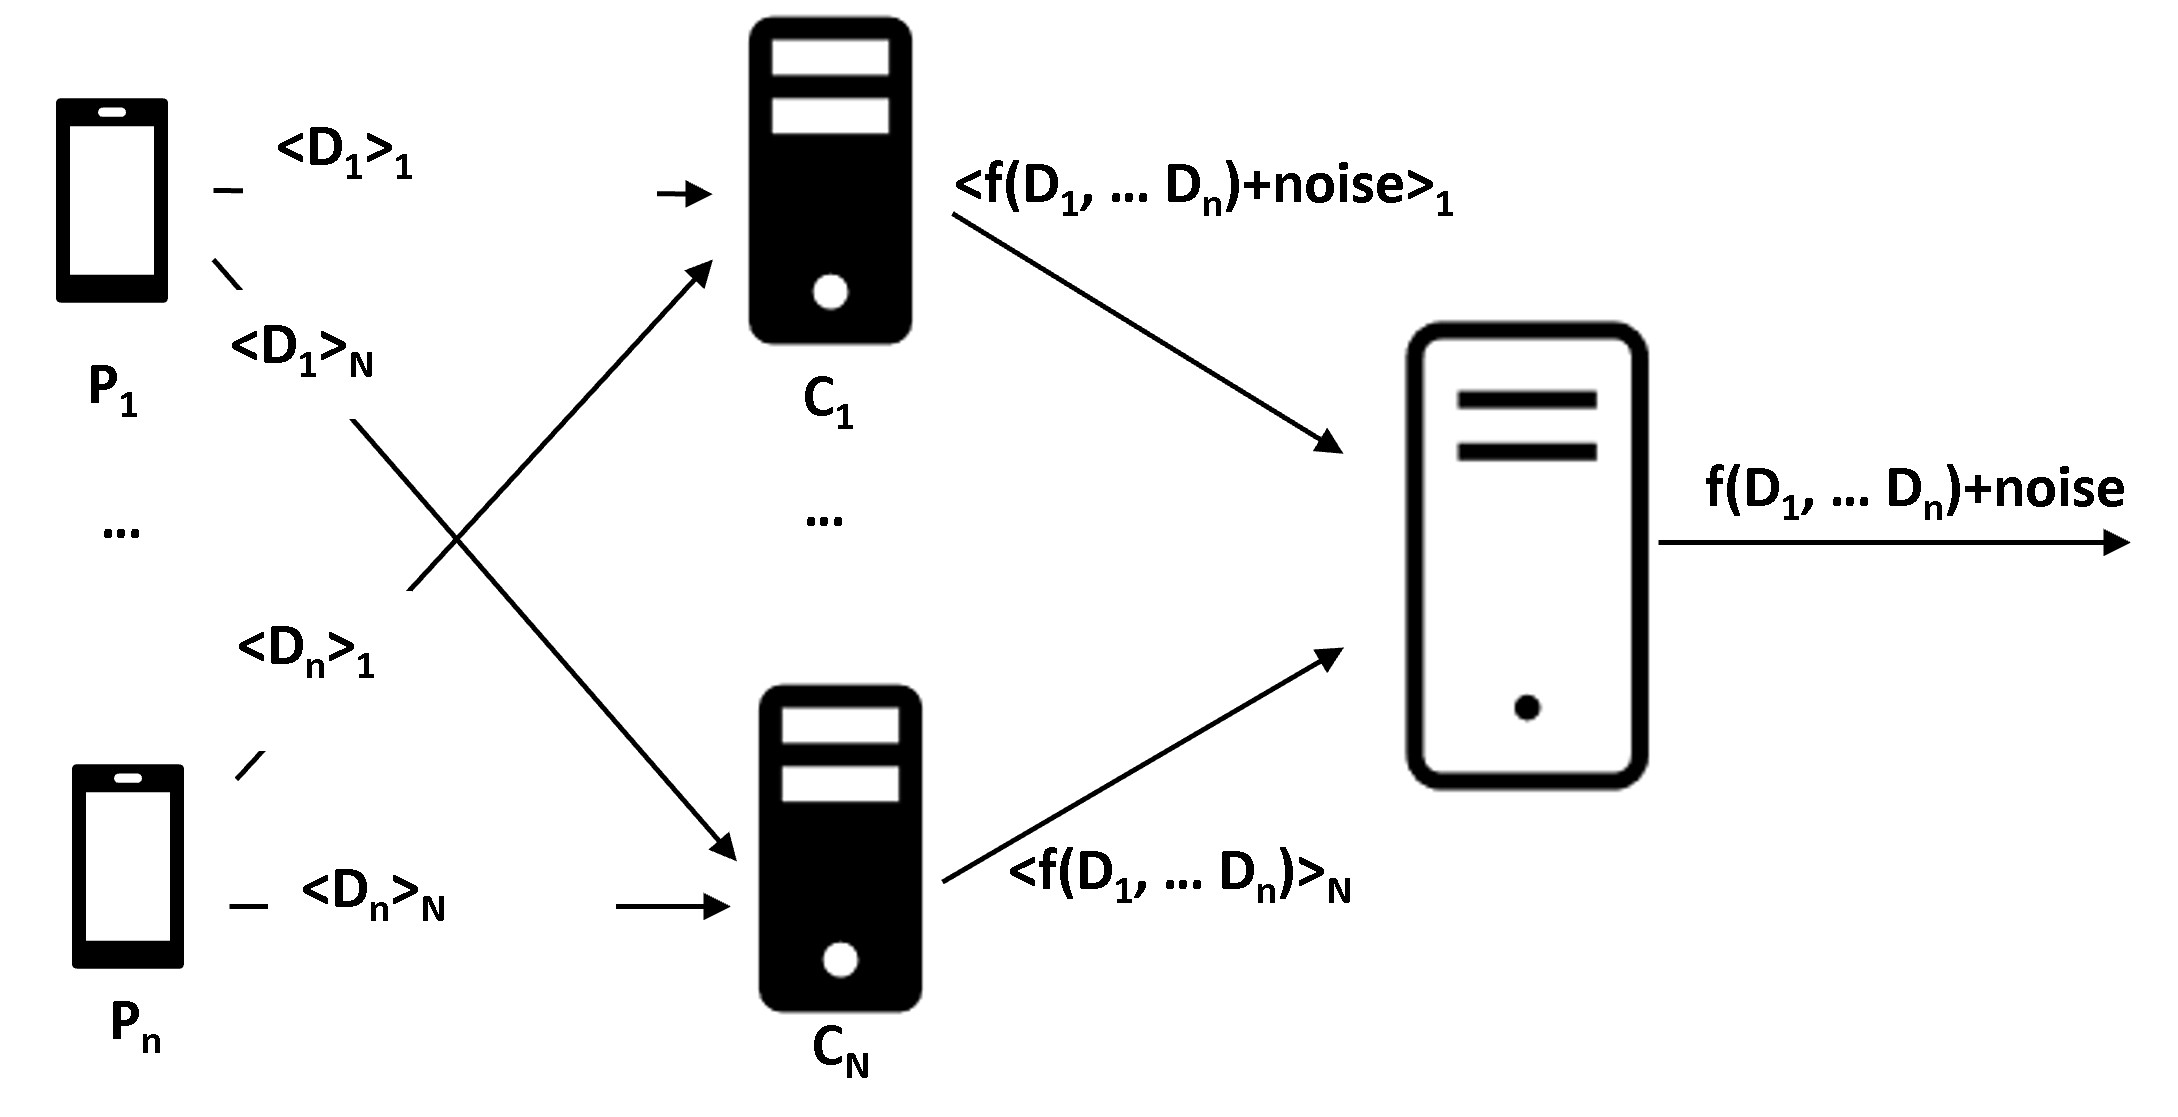
\includegraphics[width=\textwidth]{SMPC-DP procedure}
      \centering
      \caption{SMPC-DP procedure}
      \label{img:MPCDPProcedure}
\end{figure}
\FloatBarrier



% The users first secret share their private data $\left\langle D_i\right\rangle $ to the computation parties, and then, the computation parties compute $\left\langle f\left(D_1,\ldots, D_n\right) \right\rangle $, perturb the result, and send it to the reconstruction party.

% In the following parts, we first describe the \smpc building block, arithmetic operations, and the five \smpc protocols of the previous introduced differentially private mechanisms (cf.~\autoref{cha:secureDPMechanisms}).


% % Let dataset $D=\left( D_{1},\ldots, D_{n}\right) $ be distributed among $n$ parties $\left( P_{i}\right) _{i\in \left[ n\right] }$ who do not trust each other and party $P_{i}$ owns data $D_{i}$. The parties $\left(P_{i}\right)_{i \in \left[ n\right]} $ wish to jointly compute a public function $f$ on their private inputs $\left(pre\left(D_i\right)\right)_{i \in \left[ n\right]} $. After the computation, \CHANGED{either all parties or designated parties receive the result of $f\left(pre\left(D_1\right),\ldots,pre\left(D_n\right)\right)$ as output}, where $pre$ is a pre-processing function executed on their local data $\left(D_i\right)_{i \in \left[ n\right]} $. The parties want to achieve (1) computational privacy (i.e., each party's input is kept secret), \CHANGED{(2) output privacy (i.e., the output satisfies the DP),} and (3) obtain a result with reasonable accuracy.
% % \begin{enumerate}
% % 	\item The computation of $f$ should reveal nothing but the result.
% % 	\item The computation result of $f\left(pre\left(D_1\right),\ldots,pre\left(D_N\right)\right)$ should be identical to the scenario, where a trusted server has access to the whole dataset $D$ and computes $f\left( pre\left(D\right) \right)$ locally, i.e., $f\left(pre\left(D_1\right),\ldots,pre\left(D_N\right)\right)=f\left( pre(D)\right)$.
% % 	\item The result has to satisfy the differential privacy by adding it with noise, i.e., an adversary cannot infer too much information from the noisy result.
% % 	\item The noisy result can still provide statistically useful information.
% % \end{enumerate}

% % To achieve computational privacy, the parties deploy a \smpc protocol $\Uppi^{f}$ which takes $\left(pre\left(D_i\right)\right)_{i \in \left[ n\right]} $ as input and reveals only the computation result. For requirements (2) and (3), we design a SMPC-DP procedure (cf.~\autoref{prot:SMPC-DP}) which combines $\Uppi^{f}$ with a secure differentially private mechanism. Note that in following, we omit the data pre-processing procedure $pre\left(\cdot\right) $ for simplicity and use $f\left( D\right)$ to represent $f\left(D_1,\ldots,D_n\right)$.

% % Let's consider a trival example that combines \smpc protocols with a differentially private mechanism. Suppose the parties $\left(P_{i}\right)_{i \in \left[ n\right]} $ wish to calculate the sum of their local data $\left(D_{i}\right)_{i \in \left[ n\right]} $ with a publicly known function $f\left(D_1,\ldots,D_n\right)=\sum_{j=1}^{n} D_j$, and $f$ has $\ell_2$-\textit{sensitivity} $\Delta^{\left(f\right) } _2=1$ (cf.~\autoref{def:sensitivity}). Meanwhile, the parties require that only the computation result of $f$ should be revealed and differential privacy must be satisfied. To achieve this, each party first adds noise $r_i$ to its local data $D_i$ and determines $ y_{i}=D_{i} +r_{i}$. Recall that in \autoref{def:gaussianMechanism}, we have showed that $ y_{i}=$ satisfies $\left(\varepsilon ,\delta \right) $-DP for $r_i \sim \mathcal{N}\left( 0,\sigma ^{2}\right) $, where $\sigma ^{2}=\frac{2}{\varepsilon ^2}\cdot\ln\left(\frac{1.25}{\delta }\right)$ and $i\in \left[n\right] $. Then, the parties jointly run the \smpc protocol $\Uppi^{f}$ with their private inputs $y_i$ to compute function $f$. After reconstruction they get $y=\sum_{j=1}^{n} y_j=\sum_{j=1}^{n}\left( D_j+ r_j\right)$. Because of the infinite divisibility of the normal distribution~\cite{patel1996handbook}, we have $\sum_{j=1}^{n} r_j \sim \mathcal{N}\left( 0,\sigma_{sum} ^{2}\right) $ for $\sigma_{sum} ^{2}=\sum ^{n}_{j=1}\sigma ^{2}$. Therefore, the computation result $y$ satisfies $\left(\frac{\varepsilon}{\sqrt{n}},\delta \right) $-DP.

% % In general, the parties in above example can achieve $\left(\frac{\varepsilon}{\sqrt{n}},\delta \right) $-DP assuming no corrupted parties. However, in realistic scenarios, corrupted parties may try to extract information of certain parties by weaking the achieved differential privacy protection level.
% % After executing aforementioned steps honestly and obtaining the computation result $y$, the corrupted parties subtract the noise they have added from $y$. In the worst case, i.e., $n-1$ parties are corrupted, the differential privacy guarantee reduces from $\left(\frac{\varepsilon}{\sqrt{n}},\delta \right) $-DP to $\left(\varepsilon,\delta \right) $-DP. If, however, having $\left(\frac{\varepsilon}{\sqrt{n}},\delta \right) $-DP is required, a potential naive solution is that each party adds \textit{more} noise, .e.g, $r_i^{\prime} \sim \mathcal{N}\left( 0,n\cdot \sigma ^{2}\right) $, locally before running $\Uppi^{f}$. However, \CHANGED{this can lead to a severely accuracy reduction}.

% % To summarize, a well-designed SMPC-DP procedure requires a more careful integration of \smpc protocols and differentially private mechanisms. \CHANGED{To guarantee the both the accuracy and privacy, we define several requirements, that is based on the "ideal scenario" with a centralized data server, i.e., a trusted server that has access to all the parties' data $D$ locally computes $f\left( D\right) $ before adding an essential amount of noise to guarantee DP}:

% % \begin{enumerate}
% % 	\item The SMPC-DP procedure should achieve the same privacy protection level as in the centralized data server scenario, and the amount of noise $r$ (in above example: $r=\sum_{j=1}^{n} r_j$) should \CHANGED{exactly match that of the centralized data server scenario}.
% % 	\item The DP guarantee of the SMPC-DP procedure should not degenerate in the presence of corrupted parties.
% % \end{enumerate}

% % \textbf{SMPC-DP Procedure} It can be used among $n$ parties, or in an outsourcing scenario, i.e., an arbitrary amount of parties secret share their private inputs to $N$ ($N\ll n$) non-colluding computing parties. Then, the computing parties execute the $N$-party SMPC-DP protocol, where they compute $f$ and add noise shares to get the noisy secret-shared results. Finally, the noisy secret-shared results are sent back to the parties for reconstruction. We assume semi-honest adversaries that follow the protocol specifications but wish to infer additional information\cite[Chapter 2]{evans2017pragmatic}.

% % Specifically, for $i\in \left[ n\right]$, party $P_{i} $ secret shares his inputs $D_i$ to $N$ computing parties $P_{0},\ldots,P_{N}$. For $j\in \left[ N\right]$, computing party $P_j$ runs \smpc protocols for function $f$ with other computing parties using his secret-shared value $\left\langle D_1 \right\rangle _{j},\ldots,\left\langle D_n \right\rangle _{j} $ (received from $n$ parties) and get $\left\langle f\left(D\right) \right\rangle _j$. Then, computing party $P_j$ runs the \smpc protocols for distributed noise generation (DNG) with other computing parties and get a secret-shared noise $\left\langle r\right\rangle_j $. Finally, computing party $P_j$ perturbs $\left\langle f\left(D\right) \right\rangle _j$ by computing $\left\langle M\left(D\right)\right\rangle_j=\Uppi^{Perturbation}\left(\left\langle f\left(D\right) \right\rangle_j+\left\langle r\right\rangle_j\right) $ and sends it to the parties responsible for the reconstruction. Note that during the distributed noise generation, each computing party only gets a secret-shared noise $\left\langle r\right\rangle $ and even $N-1$ colluding computing parties cannot reconstruct the noise $r$. After the reconstruction, only the perturbed (noisy) result $M\left(D\right)=\text{Perturb}\left(f\left(D\right)+r\right)  $ is revealed which computes function $f$ and guarantees differential privacy. More important is that we prevent excessive noise and ensure utility since the noise $r$ is generated by all the parties instead of by each party independently (as in the above example).


% % ~\autoref{prot:SMPC-DP} describes outsourcing scenario of the SMPC-DP procedure. Note that the parties calculate $\left\langle f\left(D\right)\right\rangle =\Uppi^{f }\left(\left\langle D_1 \right\rangle ,\ldots,\left\langle D_n \right\rangle\right) $ and add the securely generated noise $\left\langle r\right\rangle$ (output perturbation) to guarantee DP. In this work, we assume that each party has computed $\left\langle f\left(D\right) \right\rangle$ and focus on the process of $\Uppi^{Noise }$, i.e., distributed noise generation (DNG).

% % \begin{protocol}[tbh!]
% % 	\centering
% % 	\fbox{
% % 		\pseudocode[space=none, syntaxhighlight=auto, addkeywords={Protocol, Input, Output},linenumbering, skipfirstln, head=\textbf{Protocol: $\Uppi^{SMPC-DP}\left(\left\langle D_1 \right\rangle ,\ldots,\left\langle D_n \right\rangle\right) $}]{
% % 			\textbf{Input: $\left\langle D_1 \right\rangle ,\ldots,\left\langle D_n \right\rangle$ } \pcskipln \\
% % 			\textbf{Output: $\left\langle M\left(D\right)\right\rangle=\left\langle f\left(D\right) \right\rangle +\left\langle r\right\rangle$} \\
% % 			\text{$\left\langle f\left(D\right)\right\rangle \gets \Uppi^{f }\left(\left\langle D_1 \right\rangle ,\ldots,\left\langle D_n \right\rangle\right) $.}\\
% % 			\text{$\left\langle r\right\rangle \gets \Uppi^{Noise } $}\\
% % 			\text{$\left\langle M\left(D\right)\right\rangle\gets \Uppi^{Perturb}\left(\left\langle f\left(D\right) \right\rangle,\left\langle r\right\rangle\right) $}
% % 		}}
% % 	\caption{SMPC-DP procedure.}
% % 	\label{prot:SMPC-DP}
% % \end{protocol}
% % \FloatBarrier



\section{Building Blocks}
\label{sec:MPCBuildingBlocks}
We construct \smpc protocols based on the following building blocks (details can be found in \autoref{app:MPCBuildingBlocks}):

\begin{enumerate}

      % \item $\left\langle \boldsymbol{y}\right\rangle^B \gets \Uppi^{RandBits}\left(\ell\right) $ allows parties to generate shares of a publicly unknown random $\ell$-bit string $\left\langle \boldsymbol{y}\right\rangle^B =\left( \left\langle y_{0}\right\rangle^B ,\ldots ,\left\langle y_{\ell-1}\right\rangle ^B\right)$ without interactive operation. Specifically, each party

      % \item $\left\langle \boldsymbol{y}\right\rangle^B \gets \Uppi^{PreOr}\left(\left\langle \boldsymbol{x}\right\rangle ^B\right) $ computes the prefix-OR of an $\ell$-bit string $\left\langle \boldsymbol{x}\right\rangle^B= \left(\left\langle x_{0}\right\rangle ^B,\ldots, \left\langle x_{\ell-1}\right\rangle ^B\right) $ and output $\left\langle \boldsymbol{y}\right\rangle^B= \left(\left\langle y_{0}\right\rangle ^B,\ldots, \left\langle y_{\ell-1}\right\rangle ^B\right) $ such that $\left\langle y_{j}\right\rangle^B = \lor _{k=0}^{j} \left\langle x_{k} \right\rangle ^B$ for $j \in \left[0,\ell-1\right] $, where $\left\langle y_{0}\right\rangle^B =\left\langle x_{0} \right\rangle ^B$.
      \item $\left\langle \boldsymbol{y}\right\rangle^B \gets \Uppi^{PreOr}\left(\left\langle \boldsymbol{x}\right\rangle ^B\right) $ computes the prefix-OR of an $\ell$-bit string $ \boldsymbol{x}= \left( x_{0},\ldots,  x_{\ell-1}\right) $ and output $\left\langle \boldsymbol{y}\right\rangle^B= \left(\left\langle y_{0}\right\rangle ^B,\ldots, \left\langle y_{\ell-1}\right\rangle ^B\right) $ such that $ y_{j} = \lor _{k=0}^{j}  x_{k} $ for $j \in \left[0,\ell-1\right] $, where $ y_{0} = x_{0} $.

      \item $\left\langle \boldsymbol{y}\right\rangle^{B} \gets \Uppi^{Geometric} $ generates shares of a geometric random variable $y\sim Geo\left(p=0.5\right) $ using \autoref{algo:Geometric}.

            % which is inspired by the OT-based multiplication algorithms~\cite{asharov2018privacy,schneider2019episode}. For example, in two-party computation, $\left\langle \boldsymbol{x}\right\rangle ^B \cdot \left\langle b\right\rangle ^B$ can be reformulated as follows:
            %       \begin{equation}
            %           \begin{split}
            %               \left\langle \boldsymbol{x}\right\rangle ^B \cdot \left\langle b\right\rangle ^B &=\left(\left\langle \boldsymbol{x}\right\rangle ^B_0\oplus \left\langle \boldsymbol{x}\right\rangle ^B_1\right)  \cdot \left(\left\langle b\right\rangle ^B_0 \oplus \left\langle b\right\rangle ^B_1 \right) \\
            %               &=\left\langle \boldsymbol{x}\right\rangle ^B_0 \cdot \left\langle b\right\rangle ^B_0 \oplus  \left\langle \boldsymbol{x}\right\rangle ^B_0 \cdot \left\langle b\right\rangle ^B_1  \oplus \left\langle \boldsymbol{x}\right\rangle ^B_1 \cdot \left\langle b\right\rangle ^B_0 \oplus  \left\langle \boldsymbol{x}\right\rangle ^B_1 \cdot \left\langle b\right\rangle ^B_1 ,
            %           \end{split}
            %       \end{equation}
            %       where $\left\langle \boldsymbol{x}\right\rangle ^B_0 \cdot \left\langle b\right\rangle ^B_0$ and $\left\langle \boldsymbol{x}\right\rangle ^B_1 \cdot \left\langle b\right\rangle ^B_1$ can be calculated by each party locally. For the remaining two mulitplications, we utilize two C-OTs (cf.~\autoref{subsubsec:OT}). For $i \in \left\{0,1\right\} $, $P_i$ inputs $\left\langle b\right\rangle ^B_i$, and $P_{1-i}$ inputs $\left(r_i, r_i\oplus \left\langle \boldsymbol{x}\right\rangle ^B_{1-i} \right) $ and receives $r_i\oplus \left(\left\langle b\right\rangle ^B_i \cdot \left\langle \boldsymbol{x}\right\rangle ^B_{1-i}\right) $, where $r_i$ is a random bit string. Finally, $P_i$ set $r_i \oplus  r_{1-i}\oplus \left(\left\langle b\right\rangle ^B_{1-i} \cdot \left\langle \boldsymbol{x}\right\rangle ^B_{i}\right)$ as its share of $\left\langle \boldsymbol{x}\right\rangle ^B_0 \cdot \left\langle b\right\rangle ^B_1  \oplus \left\langle \boldsymbol{x}\right\rangle ^B_1 \cdot \left\langle b\right\rangle ^B_0 $. We also extend $\Uppi^{OTMult}$ to multiple parties using similar C-OT based approach. We set $\Uppi^{OTMult}$ as default \smpc protocol to compute bit-vector multiplication.
            %       \TODO{check if MOTION has implemented bit-vector multiplication}

            % \item $\left(\left\langle y_1\right\rangle^B,\ldots,\left\langle y_{\ell}\right\rangle^B \right)\gets\Uppi^{Binary2Unary}\left(\left\langle \boldsymbol{x}\right\rangle ^{B},\ell\right) $~\cite{aliasgari2012secure} converts an unsigned integer $x$ from binary to unary bitwise representation and outputs an $\ell$-bit string $\boldsymbol{y}=\left( y_{0} ,\ldots , y_{\ell-1} \right) $, where the $x$ least significant bits $ y_{0} ,\ldots , y_{x-1} $ are set to $1$ and the rest bits $ y_{x} ,\ldots , y_{\ell-1} $ are set to $0$.
            % We use HyCC compiler (cf.~\autoref{subsection:MOTIONFramework}) to generate both the size-optimal and depth-optimal circuit for $\operatorname{AND}$ gate.

            % \item For signed ($INT$) and unsigned integer ($UINT$) operations (e.g., comparison, addition, substraction), we use depth-optimized circuits generated with HyCC (cf.~\autoref{subsection:MOTIONFramework}).

            % \item For floating-point operations, we use the Boolean circuits of work~\cite{demmler2015aby}.

      \item $\left\langle {y}\right\rangle ^{B,UINT}\gets \Uppi^{HW}\left(x_0,\ldots,x_{\ell}\right) $~\cite{boyar2008tight} computes the Hamming weight (i.e., the number of $1$ bits) of an $\ell$-bit string $x_0,\ldots,x_{\ell}$.
            % We first convert the input into Yao's sharing and finally convert the result back to the Boolean sharing.
            %   \TODO{better methods without share conversion???}

      \item $\left\langle \boldsymbol{y_i}\right\rangle ^{B}\gets \Uppi^{ObliviousSelection}\left(\left\langle \boldsymbol{y_0}\right\rangle^{B} ,\ldots,\left\langle \boldsymbol{y_{\ell-1}}\right\rangle^{B},\left\langle c_0\right\rangle ^B,\ldots,\left\langle c_{\ell-1}\right\rangle ^B\right) $ outputs the bit-string $\left\langle \boldsymbol{y_i}\right\rangle ^B$, where $i$ is the index of the first non-zero bit $c_{i}$ for $i\in \left[0,\ell-1\right] $. If all the bits $c_0, \ldots, c_{\ell-1}$ are zeros, bit-string $\boldsymbol{y_i} $ is set to a bit-string consisting of all zeros.

      \item $\left\langle {y}\right\rangle ^{B,UINT} \gets \Uppi^{RandInt}\left(m\right) $ generate shares of a random integer $y$ in the interval $ \left[0,m-1\right] $.

      \item $\left\langle \boldsymbol{y}\right\rangle^B \gets \Uppi^{COTMult}\left(\left\langle \boldsymbol{x}\right\rangle ^B,\left\langle b\right\rangle ^B\right) $~\cite{asharov2018privacy,schneider2019episode} computes the multiplication of a bit string $ \boldsymbol{x}$ and a single bit $ b$ with \correlatedot (cf.~\autoref{subsubsec:OT}).

      \item $\left\langle \boldsymbol{y}\right\rangle ^B \gets  \Uppi^{MUX}\left(\left\langle a\right\rangle^B, \left\langle \boldsymbol{x_0}\right\rangle^B ,\left\langle \boldsymbol{x_1}\right\rangle^B  \right) $ outputs a bit-string $\left\langle \boldsymbol{y}\right\rangle^{B} $, where $ \boldsymbol{y}=\boldsymbol{x_0} $ if $a=1$, $\boldsymbol{y}=\boldsymbol{x_1} $ otherwise.

\end{enumerate}

\section{Number Representations}
\label{sec:NumberRepresentationsandArithmeticOperations}
In \smpc, we use \booleanGMW and \arithmeticGMW protocols to implement arithmetic operations. We consider integers, fixed-point numbers, and floating-point numbers to represent the numbers in the arithmetic operations.
% We discuss the details about implementing these arithmetic operations in MOTION~\cite{braun2022motion}.
% At a high level, we use HyCC~\cite{buscher2018hycc} and CBMC-GC~\cite{buscher2016compiling} to generate depth-optimized circuits or use the available circuits from works~\cite{demmler2015aby,archer2021cost} to implement the \booleanGMW based arithmetic operations. For \arithmeticGMW based arithmetic operations, we extend the arithmetic sharing operations of MOTION~\cite{braun2022motion} to support comparison, shifting, truncation, modulo reduction, etc.

% Further, our \smpc protocols use integer, fixed-point and floating-point arithmetic interchangeably to achieve the best \smpc performance (regarding the communication and computation cost).

\paragraph{BGMW Signed/Unsigned Integer.}
The MOTION framework~\cite{braun2022motion} supports \booleanGMW unsigned integer arithmetic operations, such as $+$, $-$, $*$, $/$, and $<$. We extend it to support other arithmetic operations, e.g., modulo reduction and conversion operations with \booleanGMW fixed-point and \booleanGMW floating-point.
We also extend MOTION~\cite{braun2022motion} to support \booleanGMW signed integers with additional operations such as absolute value and negation.

% We generate depth-optimized binary circuits for \booleanGMW-based unsigned integer with HyCC~\cite{} and CBMC-GC~\cite{}.
% Except for the arithmetic operations supported by the unsigned integer, we also implement signed integer arithmetic that supports operations such as absolute value and negation.

\paragraph{BGMW Floating-Point.}
% We consider 64-bit floating-point arithmetic~\cite{IEEE754_2019}. For operations such as $+,$ $-$, $*$, $/$, $<$, square, square root, exp2, and log2, we use the binary circuits from ABY~\cite{demmler2015aby}. For other operations such as conversion operations with fixed-point and integers, ceil, floor, absolute value, round to the nearest integer, we use CBMC-GC to generate depth-optimized and size-optimized binary circuits with the C code from Berkeley SoftFloat library~\cite{BerkelySoftFloat}.
We consider $64$-bit floating-point arithmetic. For operations such as $+,$ $-$, $*$, $/$, $<$, square, square root, exp2, and log2, we use the binary circuits from ABY~\cite{demmler2015aby}. For other operations such as conversion operations with \booleanGMW fixed-point and \booleanGMW integers, ceil, floor, absolute value, round to the nearest integer, we use CBMC-GC~\cite{buscher2016compiling} to generate depth-optimized binary circuits with the C code from Berkeley SoftFloat library~\cite{BerkelySoftFloat}.

\paragraph{AGMW Floating-Point.}
\label{para:AGMWFloating-Point}
We implement the \arithmeticGMW floating-point protocols primarily based on the work of Aliasgari et al.~\cite{aliasgari2012secure}.
A floating-point number $u$ is represented as a quadruple $\left(v, p, z, s\right) $, where each term is defined as follows:
\begin{enumerate}
      \item $v\in \left[2^{\ell-1},2^{\ell}\right) $ is an $\ell$-bit mantissa (with the most significant bit always set to one),
      \item $p\in \mathbb{Z} _k$ is a $k$-bit signed exponent,
      \item $z\in \left\{0,1\right\} $ is the zero bit that is set to $1$ when $u=0$,
      \item $s\in \left\{0,1\right\}$ is the sign bit of $u$.
\end{enumerate}
This quadruple $\left(v, p, z, s\right) $ represents the value $u= \left(1-2s\right) \cdot \left(1-z\right) \cdot v \cdot 2^p$.
The \smpc protocols for floating-point in work~\cite{aliasgari2012secure} rely on the Shamir secret sharing~\cite{shamir1979share} operations performed over a prime field $\mathbb{F}_p$ (modulo $p$), whereas the arithmetic sharing operations in MOTION~\cite{braun2022motion} are performed in a ring (modulo $\mathbb{Z} _{2^{n}}$). One significant difference between finite field and ring is that there is no inverse element (i.e., $a^{-1}$ in a prime field) in the ring. The inverse operations in the work~\cite{aliasgari2012secure} are primarily for computing the logical right shifting of the shares.
Therefore, we replace the protocols that involve inverse operations in the work~\cite{aliasgari2012secure} with the \smpc protocols that support arithmetic sharing operations (e.g., logical/arithmetic right shifting, modulo reduction, etc.) over a ring from the works~\cite{escudero2020improved,dalskov2020secure,makri2021rabbit}.

\paragraph{BGMW Fixed-Point.}
% We implement fixed-point arithmetic with two precision modes:
% (i) 64-bit fixed-point with a $16$-bit fractional part,
% (ii) 64-bit fixed-point with a $31$-bit fractional part.
We implement fixed-point numbers with a $48$-bit signed integer part and a $16$-bit fractional part.
This gives us precision $2^{-16}$ and covers the values with a integer part up to $47$ bits.
We use HyCC~\cite{buscher2018hycc} to generate the depth-optimized circuits for fixed-point operations, such as $+$, $-$, $*$, $/$, and $<$.
For operations such as exp2 and log2, we use polynomial approximations~\cite{hart1978computer,aly2019benchmarking} and generate corresponding binary circuits using CBMC-GC~\cite{buscher2016compiling}.
For operations such as square root, we use both polynomial approximations~\cite{hart1978computer} and Goldschmidt approximations~\cite{markstein2004software,aly2019benchmarking}.
The main issue with fixed-point arithmetic is the inherent precision loss during arithmetic operations.
We estimate the accuracy of fixed-point exp2 operation by comparing its result to the floating-point exp2 operation with the same input.
For $1000$ random inputs in $\left[0,1\right]$, the absolute error between the fixed-point exp2 operation results and floating-point exp2 operation results are $10^{-4}\approx 2^{-13}$ in average.
% To estimate the accuracy of the fixed-point operations, we sample $1000$ values in a specific range and compare the fixed-point operation result with the floating-point operation result.
% For example, we compute the fixed-point exp2 operation with $1000$ randomly sampled values in $\left[0,1\right] $, the absolute error between fixed-point results floating-point results are $10^{-4}\approx 2^{-13}$ in average.
For log2 (with $1000$ samples in $\left[0.5,1\right] $), the absolute error is $10^{-4}\approx 2^{-13}$, and for the square root operation with polynomial or Goldschmidt approximation, the absolute error is $10^{-4}\approx 2^{-13}$.

\paragraph{AGMW Fixed-Point.}
\label{para:AGMWFixed-Point}
We implement the \arithmeticGMW fixed-point protocols primarily based on the work of Catrina and Saxena~\cite{catrina2010secure}. A fixed-point number $x$ is represented as $x = \overline{x}\cdot  2^{-f}$, where $\overline{x}$ is an $k$-bit signed integer and $f$ is the length of the fractional part.
% Specifically, $\overline{x}\in \mathbb{Z} _{\left\langle k\right\rangle }$ and $ \mathbb{Z} _{\left\langle k\right\rangle }=\left\{x\in \mathbb{Z}  \,|\,-2^{k-1}+1\leq x \leq 2^{k-1}-1\right\} $.  
We choose $\left(k,f\right)=\left(41,20\right)  $ as~\cite{aly2021scale} recommended.

\section{Random Number Generation}
\label{sec:RandomNumberGeneration}
As discussed in \autoref{cha:secureDPMechanisms}, the differentially private mechanisms rely heavily on the generation of random numbers.
Generally, four types of random numbers are used in our protocols:

\begin{enumerate}
      \item random \booleanGMW bits,
      \item random unsigned integers in a specific range,
      \item uniform random fixed in range $\left(0,1\right) $,
      \item uniform random floating-point numbers in range $\left(0,1\right) $.
\end{enumerate}

\paragraph{Random Bit String.}
As \autoref{prot:RandBits} shows, to generate a random \booleanGMW $\ell$-bit string $\left\langle \boldsymbol{b}\right\rangle^B $ in a $N$-party setting, each computation party locally generates a uniform random $\ell$-bit string $\boldsymbol{r_i}$ and set $\left\langle \boldsymbol{b}\right\rangle^B_i \gets \boldsymbol{r_i}^B$.
%  as a \booleanGMW sharing of a publicly unknown random bit string that equals to $ \bigoplus _{i=0}^{N-1}\boldsymbol{r_0}   $.
% Let $\Uppi^{RandBits}\left(\ell\right) $ denote the \smpc protocol for generating random bits of length $\ell$.

\begin{protocol}[tbh!]
      \centering
      \fbox{
      \pseudocode[space=none, syntaxhighlight=auto, addkeywords={Protocol, Input, Output},linenumbering, skipfirstln, head=\textbf{Protocol: $\Uppi^{RandBits}\left(\ell\right) $}]{
      \textbf{Input: $\ell$} \pcskipln \\
      \textbf{Output: $\left\langle \boldsymbol{b}\right\rangle ^{B}$, where $\boldsymbol{b} \sample \left\{0,1\right\}^{\ell} $} \\
      \text{Each party $P_i$ locally samples $\boldsymbol{r_i} \sample \left\{0,1\right\}^{\ell}$}\\
      \text{Set $\left\langle \boldsymbol{b}\right\rangle^B_i \gets \boldsymbol{r_i}$}
      }}
      \caption{SMCP protocol for sampling random bit-string.}
      \label{prot:RandBits}
\end{protocol}
\FloatBarrier

The other three types of random numbers are generated based on random Boolean bits with additional conversion.

\paragraph{Random Unsigned Integer.}
To generate a random unsigned integer in range $\left(0,m\right) $, we use the Simple Modular Method~\cite{NISTRandomNumber2015}, that first generates an uniform random $\ell$-bit string $\left\langle \boldsymbol{r}\right\rangle^B $ ($\ell=128$ or $\ell=256$), and computes $ \left\langle \boldsymbol{r}\right\rangle^B \mod m$ by taking $\left\langle \boldsymbol{r}\right\rangle^B $ as an $\ell$-bit unsigned integer. We keep the security parameter $s=\ell-\log_2 m$ greater than $64$ by limiting $m<2^{64}$.

\paragraph{Uniform Random Fixed-Point Numbers.}
Suppose the fixed-point numbers have $f$ fractional bits and $k-f$ integer bits.
To generate such a uniform random fixed-point number in the range $\left[0,1\right)$, we first generate $f$ random bits and set it as the fractional part of the random fixed-point number and fill the $\left(k-f\right) $-bit integer part with zero bits.

                  \paragraph{Uniform Random Floating-Point Numbers.}
                  To generate a uniform random floating point in range $\left(0,1\right) $, we follow \autoref{algo:RandFloat1} and construct corresponding \smpc protocol \autoref{prot:RandFloat1}.
                  We first generate shares of the mantissa bits $\left\langle d_{1}\right\rangle^{B}, \ldots ,\left\langle d_{52}\right\rangle ^{B} $ with $\Uppi^{RandBits}\left(52\right) $, and generate shares of a geometric random variable $\left\langle {x}\right\rangle^{B,UINT} $ with $\Uppi^{Geometric}\left(0.5\right) $ to build the biased exponent $\left\langle {e}\right\rangle^{B,UINT}$, where $e=1023-\left(x+1\right) $. Finally, the parties use the mantissa and exponent bits to build the floating-point number $U=\left(1.d_{1} \ldots d_{52}\right)_{2} \times 2^{e -1023} $.

                  \begin{protocol}[tbh!]
                        \centering
                        \fbox{
                              \pseudocode[space=none, syntaxhighlight=auto, addkeywords={Protocol, Input, Output},linenumbering, skipfirstln, head=\textbf{Protocol: $\Uppi^{RandFloat1}$}]{
                                    \textbf{Input: None} \pcskipln \\
                                    \textbf{Output: $\left\langle {U}\right\rangle ^{B,FL}$, where $U=\left(1.d_{1} \ldots d_{52}\right)_{2} \times 2^{e -1023} $} \\
                                    \text{$\left(\left\langle d_{1}\right\rangle ^B ,\ldots ,\left\langle d_{52}\right\rangle^B\right) \gets \Uppi^{RandBits}\left(52\right) $} \\
                                    \text{$\left\langle {x}\right\rangle ^{B,UINT} \gets \Uppi^{Geometric}\left(0.5\right)  $} \\
                                    \text{$\left\langle {e} \right\rangle^{B,UINT}\gets 1023-\left(\left\langle {x}\right\rangle^{B,UINT}+1\right)  $} \\
                                    \text{$U\gets\left(1.d_{1} \ldots d_{52}\right)_{2} \times 2^{e -1023} $}
                              }}
                        \caption{SMCP protocol for sampling uniform random floating-point $U\in \mathbb{D} \cap \left(0,1\right) $.}
                        \label{prot:RandFloat1}
                  \end{protocol}
                  \FloatBarrier


                  \section{\smpc Protocols for Snapping Mechanism}
                  \label{sec:MPCProtocolsforSnappingMechanism}

                  % \textbf{General Overview.}
                  Recall that the snapping mechanism (cf.~\autoref{sec:snappingMechanism}) is defined as follows:
                  \begin{equation}
                        \begin{split}
                              M_{S}\left(f\left(D\right),\lambda,B\right) =\text{clamp}_{B}\left(\left\lfloor\text {clamp }_{B}\left(f\left(D\right) \right) \oplus S\otimes \lambda\otimes \text{LN}\left(U\right) \right\rceil_{\Lambda}\right).
                        \end{split}
                  \end{equation}

                  The \smpc protocol for the snapping mechanism is to unfold the mathematical operations and replaces them with the corresponding \smpc protocols. We reformulate $M_{S}\left(f\left(D\right),\lambda,B\right)$ in secret sharing form as follows:
                  \begin{equation}
                        \label{eq:snappingMPC}
                        \left\langle M_{S}\left(f\left(D\right) ,\lambda,B\right)\right\rangle =\text{clamp}_{B}\left(\left\lfloor\text {clamp }_{B}\left(\left\langle f\left(D\right)\right\rangle \right) \oplus \left\langle S\right\rangle \otimes \lambda\otimes \text{LN}\left(\left\langle U\right\rangle \right) \right\rceil_{\Lambda}\right).
                  \end{equation}

                  % We assume that the computation parties has already computed the query function $\left\langle f\left(D\right)\right\rangle$. 
                  % $\left\langle S\right\rangle \otimes \lambda\otimes \text{LN}\left(\left\langle U^{*}\right\rangle \right)$ is the share of noise.
                  Parameters $\lambda $, $\Lambda$, and $B$ are publicly known. The random sign $ S\in \left\{0,1\right\}$ and the random floating-point number $ U\in \left(0,1\right)  $ can be generated with \autoref{prot:RandBits} and \autoref{prot:RandFloat1}.
                  Floating-point operations such as natural logarithm operation $LN\left(\cdot\right) $, addition ($\oplus$) and multiplication ($\otimes$) are available in both \booleanGMW and \arithmeticGMW protocols.
                  % Operation $\left\lfloor \left\langle x\right\rangle \right\rceil_{\Lambda} $ rounds input $x$ to the nearest multiple of $\Lambda$ (a publicly known value).
                  % The plaintext implementation of $\left\lfloor x\right\rceil_{\Lambda} $ can be found in Covington's work~\cite{Covington2019}, that relies on the bit manipulation of floating-point~\cite{IEEE754_2019}. Therefore, we choose BGMW floating-point arithmetic and generate depth-optimized circuits with CBMC-GC for operation $\left\lfloor \left\langle x\right\rangle \right\rceil_{\Lambda} $.
                  Covington~\cite{Covington2019} provided a plaintext implementation of function $\left\lfloor x\right\rceil_{\Lambda} $ that relies on the bit manipulation of the binary representation of floating-point numbers.
                  Therefore, we choose \booleanGMW protocols and generate corresponding depth-optimized circuits with CBMC-GC~\cite{buscher2016compiling}.
                  The \booleanGMW protocol of function $\left\lfloor \left\langle x\right\rangle \right\rceil_{\Lambda} $ is denoted by $\Uppi^{RoundToLambda}$.
                  \autoref{prot:ClampB} provides an implementation of function $\text{clamp}_{B}$ (cf.~\autoref{sec:snappingMechanism}) using \booleanGMW floating-point arithmetic operations.

                  \begin{protocol}[tbh!]
                        \centering
                        \fbox{
                              \pseudocode[space=none, syntaxhighlight=auto, addkeywords={Protocol, Input, Output},linenumbering, skipfirstln, head=\textbf{Protocol: $\Uppi^{ClampB}\left(\left\langle {x}\right\rangle^{B,FL},B\right) $}]{
                                    \textbf{Input: $\left\langle {x}\right\rangle^{B,FL}$, $B$} \pcskipln \\
                                    \textbf{Output: $\left\langle {x_{clampB}}\right\rangle^{B,FL}$} \\
                                    \text{$\left\langle cond_{\left\lvert x\right\rvert <B}\right\rangle^B \gets \Uppi^{FL\_Lt}\left(\Uppi^{FL\_Abs}\left(\left\langle {x} \right\rangle^{B,FL}\right) ,B\right) $}\\
                                    \text{ $\left\langle {x_{clampB}}\right\rangle^{B,FL}\gets \Uppi^{MUX}\left(\left\langle cond_{\left\lvert x\right\rvert <B}\right\rangle^B, \left\langle {x_0}\right\rangle^{B,FL} ,B  \right)$}\\
                                    \text{Extract the sign bit of $\left\langle {x}\right\rangle^{B,FL} $ and set it as the sign bit of $\left\langle {x_{clampB}}\right\rangle^{B,FL}$}
                              }}
                        \caption{\smpc protocol for $\text{clamp}_B\left(x\right) $.}
                        \label{prot:ClampB}
                  \end{protocol}
                  \FloatBarrier

                  \paragraph{SMPC Protocols for Snapping Mechanism.}
                  We integrate the sub-protocols and present the \booleanGMW protocol for the snapping mechanism in \autoref{prot:SnappingMechanism}. We assume that the query function $\left\langle f\left(D\right) \right\rangle^{B,FL} $ is already computed.

                  \begin{protocol}[tbh!]
                        \centering
                        \fbox{
                        \pseudocode[space=none, syntaxhighlight=auto, addkeywords={Protocol, Input, Output},linenumbering, skipfirstln, head=\textbf{Protocol: $\Uppi^{SnappingMechanism}\left(\left\langle {f\left(D\right)}\right\rangle^{B,FL}  ,\lambda,B,n, \Lambda\right) $}]{
                        \textbf{Input: $\left\langle {f\left(D\right)}\right\rangle^{B,FL}$, $\lambda$, $B$, $n$, $\Lambda$} \pcskipln \\
                        \textbf{Output: $\left\langle {x_{SM}}\right\rangle ^{B,FL}$, where $x_{SM}=M_{S}\left( f\left(D\right) ,\lambda,B\right)$} \\
                        \text{$\left\langle {U}\right\rangle ^{B,FL}\gets\Uppi^{RandFloat1}$}\\
                        \text{$\left\langle S\right\rangle ^B \gets\Uppi^{RandBits}\left(1\right) $}\\
                        \text{$\left\langle {f\left(D\right)_{clampB}} \right\rangle ^{B,FL} \gets\Uppi^{ClampB}\left(\left\langle {f\left(D\right) }\right\rangle^{B,FL},B\right) $}\\
                        \text{$ \left\langle {Y_{LapNoise}}\right\rangle ^{B,FL}=\Uppi^{FL\_Mul}\left(\lambda ,\Uppi^{FL\_Ln}\left(\left\langle {U}\right\rangle ^{B,FL}\right)\right)  $}\\
                        \text{Set $\left\langle S\right\rangle^B $ as the sign bit of $\left\langle {Y_{LapNoise}}\right\rangle ^{B,FL}$}\\
                        % \text{$\left\langle S_{Y_{LapNoise}}\right\rangle ^{B}\gets \left\langle S_{Y_{LapNoise}}^{\prime}\right\rangle ^{B}$}\\
                        \text{$ \left\langle {x}\right\rangle ^{B,FL}\gets \Uppi^{FL\_Add}\left(\left\langle {f\left(D\right)_{clampB}} \right\rangle ^{B,FL},\left\langle {Y_{LapNoise}}\right\rangle ^{B,FL}\right) $}\\
                        \text{$\left\langle {\left\lfloor x\right\rceil_\Lambda  }\right\rangle ^{B,FL} \gets \Uppi^{RoundToLambda}\left(\left\langle {x}\right\rangle^{B,FL},\Lambda\right) $}\\
                        \text{$\left\langle {x_{SM}}\right\rangle ^{B,FL}\gets \Uppi^{ClampB}\left(\left\langle {\left\lfloor x\right\rceil_\Lambda  }\right\rangle ^{B,FL},B\right)$}
                        }}
                        \caption{SMPC protocol for snapping mechanism (\booleanGMW).}
                        \label{prot:SnappingMechanism}
                  \end{protocol}
                  \FloatBarrier


                  % The parties generate the noise starting from the generation of random variable $S\in \left\{-1,1\right\} $ and $U^{*} \in \mathbb{D} \cap \left(0,1\right)$. Finally, the parties compute $\left\lfloor \cdot \right\rceil_{\Lambda}$ and $\text{clamp}_{B}\left(\cdot\right) $.

                  % According to our SMPC-DP procedure (cf.~\autoref{cha:ProcedureMPCDP}), the parties generate a noise share $\left\langle r\right\rangle$ and add it to $\left\langle f\left(D\right)\right\rangle$ to achieve differential privacy (cf.~\autoref{sec:differentialPrivacy}). 


                  % In our \smpc protocols, we mainly operate on IEEE 754 floating-point (cf.~\autoref{subsubsec:floatingPoint}): $\left\langle \boldsymbol{x}\right\rangle^{B,FL} =\left(\left\langle S\right\rangle ,\left\langle d_1\right\rangle,\ldots,\left\langle d_{52}\right\rangle, \left\langle e_1\right\rangle,\ldots,\left\langle e_{11}\right\rangle\right) $, where $x = \left(-1\right)^S \left(1.d_{1} \hdots d_{52}\right)_2 \times 2^{\left(e_1 \hdots e_{11}\right)_2-1023} $.

                  % \subsection{Generation of $U^{*}$ and $S$}

                  % Each party can generate sign $\left\langle S\right\rangle ^B $ by sampling a random bit locally.

                  % As discussed in~\autoref{subsubsec:generationUStar}, $U^{*}$ is the uniform distribution over $\mathbb{D} \cap \left(0,1\right) $, which can be represented in IEEE-754 double-precision floating-point (cf.~\autoref{subsubsec:floatingPoint}) as follows:

                  % \[U^{*}=\left(1.d_{1}\ldots d_{52}\right)_{2}\times 2^{e-1023},\]
                  % where significant bits $\left(d_{1},\ldots ,d_{52}\right) $ are sampled uniformly from $\left\{0,1\right\}^{52} $ and biased exponent $x=e-1023$ is sampled from a geometric distribution (cf.~\autoref{def:GeometricDistribution}).

                  % As~\autoref{prot:RandFloat1} shows, we first generate significand bits share $\left\langle d_{1}\right\rangle^{B}, \ldots ,\left\langle d_{52}\right\rangle ^{B} $ with $\Uppi^{RandBits}\left(52\right) $ (cf.~\autoref{sec:MPCBuildingBlocks}), then generate a geometric random variable share $\left\langle \boldsymbol{x}\right\rangle^{B,UINT} $ with $\Uppi^{Geometric}$ (cf.~\autoref{prot:GeometricDistribution}) to build the biased exponent $\left\langle \boldsymbol{x}\right\rangle^{B,UINT}$, where $x=e-1023$. Finally, the parties compute and obtain shares of the floating-point number $U^{*}=\left(1.d_{1} \ldots d_{52}\right)_{2} \times 2^{e -1023} $.




                  % \subsection{Calculation of $\left\lfloor \cdot\right\rceil_{\Lambda} $}

                  % \autoref{prot:Round2Delta} rounds $x$ to the nearest multiply of $\Lambda=2^n$.
                  % As discussed in~\autoref{subsubsec:roundX2Lambda}, $\lfloor x \rceil_{\Lambda}$ with input $x$ can be calculated in three steps:
                  % \begin{enumerate}
                  %     \item $x^{\prime} = \frac{x}{\Lambda}$
                  %     \item Round $x^{\prime}$ to the nearest integer, yielding $x^{\prime\prime}$
                  %     \item $\lfloor x \rceil_{\Lambda} = \Lambda \cdot x^{\prime\prime}$
                  % \end{enumerate}

                  % % In line $1$, the parties expand the biased exponent to $e=\left(0,e_1,\ldots,e_{11}\right) $ because $y$ (line $4$) is in the interval $\left[-1022,1023\right] $.
                  % In line $1$, the parties extended biased exponent to $\left(0,\left\langle e_1\right\rangle,\ldots,\left\langle e_{11}\right\rangle\right)  $ such that $\left\langle \boldsymbol{e}\right\rangle^{B,UINT}$ has enough bits to represent a $12$-bit signed integer.
                  % In line $2$, the parties convert biased exponent $\left(e_1,\ldots,e_{11}\right) _2$ to signed integer because $\left(e_1,\ldots,e_{11}\right) _2-n-1023$ (line $3$) can be smaller than $0$ but unsigned integer cannot represent a negative value.
                  % In line $3,4$, the parties compute $\left(e_1,\ldots,e_{11}\right) _2-n-1023$ that is equivalent to $x^{\prime}=\frac{x}{\Lambda}$.
                  % In line $5,6,8,16,17,19,20,22$, we compute the conditions for five cases as discussed in~\autoref{para:roundX2Int}. In line $9$, the parties run $\Uppi^{Binary2Unary}\left(\left\langle \boldsymbol{y}\right\rangle ^{B,UINT},52\right)$ to get $p_1,\ldots,p_{52}$, where $p_j=1$ for $j \in \left[y\right] $ and other bits equal to zero.
                  % In line $10$, the parties extract the first $y$ bits from significant field $(d_1,\ldots,d_{52})$, set the rest bits to zero, and obtain $\left(d_1,\ldots,d_y,\overline{0}_{52-y}\right) $.
                  % In line $11-13$, the parties extract $d_{y+1}$ by setting all bits in bit string $c$ to zero except $c_{y+1}=1$.
                  % In line $14$, the parties verify if $\left(d_1,\ldots,d_{y}\right)=\left(0,\ldots,0\right)  $, and set is as the subcondition for Case 3.
                  % In line $15$, the parties calculate the new significant bits for Case 3a.
                  % In line $18$, the parties compute the biased exponent for Case 3b.
                  % In line $21$, the parties set the biased exponent for Case 4.

                  % % \label{subsubsec:significantBitsAndBiasedExponentM}
                  % In line $23$, the parties compute the significant bits $\left\langle \boldsymbol{t}\right\rangle^{B,UINT}$ and biased exponent $\left\langle\boldsymbol {m}\right\rangle^{B,UINT} $ with $\Uppi^{OTMult}$ (cf.~\autoref{sec:MPCBuildingBlocks}) as follows:


                  % \begin{equation}
                  %     \label{equ:significantBitsT}
                  %     \begin{split}
                  %         \left\langle \boldsymbol{t}\right\rangle^{B,UINT} =  \quad & \left\langle cond_{case1}\right\rangle ^{B}\cdot \left(\left\langle d_1\right\rangle^B ,\ldots,\left\langle d_{52}\right\rangle ^B\right) \\
                  %         \oplus & \left\langle cond_{case3a}\right\rangle ^B \cdot \left\langle \boldsymbol{d_{case3a}}\right\rangle ^{B,UINT}\\
                  %         \oplus &\left\langle cond_{case3c}\right\rangle ^B\cdot\left\langle \boldsymbol{d_{case3c}}\right\rangle ^{B,UINT},
                  %         % \\
                  %         % \oplus &\left(\left\langle cond_{case2}\right\rangle^B \oplus\left\langle cond_{case3b}\right\rangle ^B\oplus\left\langle cond_{case4}\right\rangle ^B\oplus\left\langle cond_{case5}\right\rangle ^B \right) \cdot\left\langle \boldsymbol{d_{\overline{0}_{\left(52\right) }}}\right\rangle^{B,UINT}
                  %     \end{split}
                  % \end{equation} 

                  % \begin{equation}
                  %     \label{equ:biasedExponentM}
                  %     \begin{split}
                  %         \left\langle\boldsymbol {m}\right\rangle^{B,UINT} = \quad & \left(\left\langle cond_{case1}\right\rangle^B\oplus\left\langle cond_{case3a}\right\rangle^B \oplus \left\langle cond_{case3c}\right\rangle^B\right)\cdot\left(\left\langle e_1\right\rangle ^{B},\ldots,\left\langle e_{11}\right\rangle ^{B}\right)  \\
                  %         \oplus &\left\langle cond_{case2}\right\rangle^B\cdot\left\langle \boldsymbol{m_{case2}}\right\rangle^{B,UINT}\\
                  %         \oplus&\left\langle cond_{case3b}\right\rangle^B\cdot\left\langle \boldsymbol{m_{case3b }}\right\rangle ^{B,UINT}\\
                  %         \oplus&\left\langle cond_{case4}\right\rangle^B\cdot\left\langle \boldsymbol{m_{case4}}\right\rangle^{B,UINT},
                  %         % \\ 
                  %         % \oplus&\left\langle cond_{case5}\right\rangle^B\cdot\left\langle \boldsymbol{z_{\overline{0}_{\left(11\right) }} }\right\rangle ^{B,UINT}
                  %     \end{split}
                  % \end{equation}

                  % Note that \autoref{equ:significantBitsT} ignore Case 2, Case 3b, Case 4 and Case 5, because the significant bits of those cases are all zeros. Similarly, we ignore Case 5 in~\autoref{equ:biasedExponentM}.

                  % In line $24,25$, the parties first check if $x^{\prime\prime}$ equals to zero, output $\lfloor x \rceil_{\Lambda} = \Lambda \cdot  x^{\prime\prime}$ if not, $x^{\prime\prime}$ otherwise.



                  % \begin{protocol}[tbh!]
                  %     \centering
                  %     \fbox{
                  %         \pseudocode[space=none, syntaxhighlight=auto, addkeywords={Protocol, Input, Output, FOR, TO},linenumbering, skipfirstln, head=\textbf{Protocol: $\Uppi^{Round2Lambda}\left(\left\langle \boldsymbol{x}\right\rangle^{B,FL}, n\right) $}]{
                  %             \textbf{Input: $\left\langle \boldsymbol{x}\right\rangle^{B,FL} =\left(\left\langle S\right\rangle^B ,\left\langle d_1\right\rangle^B,\ldots,\left\langle d_{52}\right\rangle^B, \left\langle e_1\right\rangle^B,\ldots,\left\langle e_{11}\right\rangle^B\right) $, $n$, where $\Lambda=2^n$} \pcskipln \\
                  %             \textbf{Output: $\left\langle \boldsymbol{\left\lfloor x\right\rceil _{\Lambda}}\right\rangle^{B,FL} =\left(\left\langle S\right\rangle^B ,\left\langle \boldsymbol{t}\right\rangle ^{B,UINT} ,\left\langle \boldsymbol{m}\right\rangle^{B,UINT}\right)$, where $\left\langle \boldsymbol{t}\right\rangle ^{B,UINT} =\left(\left\langle t_1\right\rangle^B,\ldots,\left\langle t_{11}\right\rangle^B\right)  $ and $\left\langle \boldsymbol{m}\right\rangle^{B,UINT} =\left(\left\langle m_1\right\rangle^B,\ldots,\left\langle m_{11}\right\rangle^B\right)  $}\\
                  %             \text{$\left\langle \boldsymbol{e}\right\rangle^{B,UINT} \gets \left(0,\left\langle e_1\right\rangle^B,\ldots,\left\langle e_{11}\right\rangle^B\right)  $}\\
                  %             \text{$\left\langle \boldsymbol{e}\right\rangle^{B,INT} \gets \operatorname{UI2SI}\left(\left\langle \boldsymbol{e}\right\rangle^{B,UINT}\right)  $}\\
                  %             \text{$\left\langle \boldsymbol{y}\right\rangle^{B,UINT}\gets \left\langle \boldsymbol{e}\right\rangle^{B,UINT}-n-1023$}\\
                  %             \text{$\left\langle \boldsymbol{y}\right\rangle^{B,INT}\gets \left\langle \boldsymbol{e}\right\rangle^{B,INT}-n-1023$\t\t //$x^{\prime} = \frac{x}{\Lambda}$}\\
                  %             % case 1
                  %             \text{$\left\langle cond_{case1}\right\rangle ^B\gets\left(\left\langle \boldsymbol{y}\right\rangle^{B,INT} >51\right) $\t\t // Case 1: $y\geq 52$}\\
                  %             % case 2
                  %             \text{$\left\langle cond_{case2}\right\rangle ^B\gets\left(\left\langle \boldsymbol{y}\right\rangle^{B,INT}==0\right) $\t\t // Case 2: y==0}\\
                  %             \text{$ \left\langle \boldsymbol{m_{case2}}\right\rangle^{B,UINT}\gets\operatorname{NOT}\left(\left\langle d_1\right\rangle^B\right)  \cdot 1023+\left\langle d_1\right\rangle ^B \cdot 1024$\t\t // Case 2: $m=1023+d_1$}\\
                  %             % \text{Each party locally set $\left\langle \boldsymbol{d_{\overline{0}_{\left(52\right) }}}\right\rangle^{B,UINT} =\left(\overline{0}_{\left(52\right) } \right) $}\\
                  %             % case 3
                  %             \text{$\left\langle cond_{case3}\right\rangle ^B\gets \left(\left\langle \boldsymbol{y}\right\rangle^{B,INT}>0\right) \land \operatorname{NOT} \left(\left\langle cond_{case1}\right\rangle ^B\right) $\t\t // Case 3: $y \in \left[1,51\right] $}\\
                  %             \text{$\left(\left\langle p_1\right\rangle^B,\ldots,\left\langle p_{52}\right\rangle^B \right)\gets\Uppi^{Binary2Unary}\left(\left\langle \boldsymbol{y}\right\rangle ^{B,UINT},52\right) $} \\
                  %             \text{$\left\langle \boldsymbol{d_{case3c}}\right\rangle^{B,UINT}=\left(\left\langle p_{1}\right\rangle^B \land \left\langle d_{1}\right\rangle^B,\ldots,\left\langle p_{52}\right\rangle^B \land \left\langle d_{52}\right\rangle^B\right) $}\\
                  %             \text{FOR $j =1 $ TO $51$ } \\
                  %             \text{\t\t$\left\langle c_{j+1}\right\rangle^B =\left\langle p_{j}\right\rangle^B \oplus  \left\langle p_{j+1}\right\rangle ^B$, where $\left\langle c_{1}\right\rangle ^B=0$}\\
                  %             \text{$\left\langle d_{y+1}\right\rangle^{B}=\oplus _{j = 1}^{52} \left(\left\langle c_{j}\right\rangle^B \land \left\langle d_{j}\right\rangle^B\right)  $}\\
                  %             \text{$\left\langle cond_{ d_1 \land \ldots \land d_y==1 }\right\rangle ^{B}\gets \land_{j = 1}^{52}\left( \left\langle p_j\right\rangle^B \land \left\langle d_j\right\rangle^B \right)  $\t\t // Case 3: For $i \in \left[y\right] $, $\forall i :d_i=1$}\\
                  %             \text{$\left\langle \boldsymbol{d_{case3a}}\right\rangle ^{B,UINT}\gets \left\langle \boldsymbol{d_{case3c}}\right\rangle^{B,UINT}+\text{POW2}\left(52- \left\langle \boldsymbol{y}\right\rangle^{B,UINT}\right) $\t\t// Case 3a: $\left(d_1^{\prime}\ldots d_y^{\prime}\right)_2 =\left(d_1\ldots d_y\right)_2 +1 $}\\
                  %             % case 3a
                  %             \text{$\left\langle cond_{case3a}\right\rangle ^B\gets \left\langle d_{y+1}\right\rangle ^B \land \operatorname{NOT}\left(\left\langle cond_{ d_1 \land \ldots \land d_y==1 }\right\rangle ^{B}\right) $}\\
                  %             % case 3b
                  %             \text{$\left\langle cond_{case3b}\right\rangle ^B\gets \left\langle d_{y+1}\right\rangle ^B \land \left\langle cond_{ d_1 \land \ldots \land d_y==1 }\right\rangle ^{B} $}\\
                  %             \text{$\left\langle \boldsymbol{m_{case3b}}\right\rangle^{B,UINT} \gets \left\langle \boldsymbol{y}\right\rangle^{B,UINT}+1+1023 $\t\t// Case 3b: $m=y+1+1023$}\\
                  %             % case 3c
                  %             \text{$\left\langle cond_{case3c}\right\rangle ^B\gets \text{NOT}\left(\left\langle d_{y+1}\right\rangle^B\right)  $}\\
                  %             % case 4
                  %             \text{$\left\langle cond_{case4}\right\rangle ^B\gets \left(\left\langle \boldsymbol{y}\right\rangle^{B,INT}==\left(-1\right) \right) $\t\t // Case 4: $y==-1$}\\
                  %             \text{$\left\langle \boldsymbol{m_{case4}}\right\rangle ^{B,UINT}\gets \left(0,\overline{1}_{\left(10\right) }\right) $\t\t// Case 4: $m=\left(01111111111\right)_2 $}\\
                  %             % case 5
                  %             \text{$\left\langle cond_{case5}\right\rangle ^B\gets\left(\left\langle \boldsymbol{y}\right\rangle ^{B,INT}<\left(-1\right)\right) $\t\t // Case 5: $y<-1$}\\
                  %             % \text{$\left\langle \boldsymbol{z_{\overline{0}_{\left(11\right) }}}\right\rangle^{B,UINT}=\left(\overline{0}_{\left(11\right) }\right) $}\\
                  %             % choose the correct round result
                  %             \text{$\left\langle \boldsymbol{t}\right\rangle^{B,UINT},\left\langle \boldsymbol{m}\right\rangle^{B,UINT} \gets \Uppi^{OTMult}\left(\cdot\right) $\t\t// $x^{\prime\prime}\gets \operatorname{round} x^{\prime} \text{to nearest integer}$}\\
                  %             % \text{$\left\langle \boldsymbol{t}\right\rangle^{B,UINT},\left\langle \boldsymbol{m}\right\rangle^{B,UINT} \gets \Uppi^{OTMult}\left(\cdot\right) $~\autoref{equ:significantBitsT}, \autoref{equ:ISMiddlePoint}}\\
                  %             \text{$\left\langle cond_{ x^{\prime\prime}\neq \pm 0}\right\rangle ^B\gets \left(\lor_{j=1}^{52}\left\langle t_j\right\rangle^B\right)  \lor \left(\lor_{j=1}^{11}\left\langle m_j\right\rangle^B\right)  $\t\t // check if $x^{\prime\prime}=\pm0$}\\
                  %             \text{$\left\langle \boldsymbol{m }\right\rangle^{B,UINT} \gets\left\langle cond_{ \neq \pm 0}\right\rangle ^B \land \left(\left\langle \boldsymbol{m}\right\rangle^{B,UINT}+n\right)   $\t\t// $\lfloor x \rceil_{\Lambda} = \Lambda \cdot  x^{\prime\prime}$}
                  %         }}
                  %     \caption{\smpc Protocol for $\left\lfloor x\right\rceil _\Lambda $}
                  %     \label{prot:Round2Delta}
                  % \end{protocol}
                  % \FloatBarrier


                  % \subsection{SMPC-DP Protocol for Snapping Mechanism}
                  % \autoref{prot:SnappingMechanism} integrates our \smpc protocols for snapping mechanism in~\autoref{sec:snappingMPC} into SMPC-DP procedure (cf.~\autoref{cha:ProcedureMPCDP}).
                  % Recall (cf.~\autoref{eq:snappingMPC})
                  % \[\left\langle M_{S}\left( f\left(D\right) ,\lambda,B\right)\right\rangle =\text{clamp}_{B}\left(\left\lfloor\text {clamp }_{B}\left(\left\langle f\left(D\right)\right\rangle \right) \oplus \left\langle S\right\rangle \otimes \lambda\otimes \text{LN}\left(\left\langle U^{*}\right\rangle \right) \right\rceil_{\Lambda}\right).\]
                  % \end{equation}

                  % $\Lambda=2^n$ and can be calculated from the publicly known $\lambda$ (cf.~\autoref{subsubsec:calLambda}) without \smpc.
                  % In line $5$, we directly manipulate sign bit of $\left\langle \boldsymbol{Y_{LapNoise}}\right\rangle ^{B,FL} $.




                  % \section{\smpc Protocols for Integer-scaling Mechanism}
                  % In this section, we construct \smpc protocols for Integer-Scaling Laplace mechanism (cf.~\autoref{sec:IntegerScalingLaplaceMechanism}) and Integer-Scaling Gaussian mechanism (cf.~\autoref{subsec:ISGauss}).

                  \section{SMPC Protocols for Integer-Scaling Laplace Mechanism}
                  \label{sec:MPCProtocolsforInteger-ScalingLaplaceMechanism}
                  Recall that the Integer-Scaling Laplace mechanism $M_{ISLap}\left(f\left(D\right),r,\varepsilon,\Delta _r\right)=f_r\left(D\right) +ir$ (cf.~\autoref{subsec:ISLap}) re-scales a discrete Laplace random variable $i \sim DLap\left(t=\frac{\Delta_r}{r\varepsilon}\right) $ to simulate a continuous Laplace random variable, where $i$ can be generated with \autoref{algo:GeometricExpBinarySearch} and \autoref{algo:TwoSideGeometric}. We provide the \smpc protocols for both sampling algorithms and the Integer-Scaling Laplace mechanism in the following part.

                  \subsubsection{SMPC Protocols for Binary Search Based Geometric Sampling Algorithm}
                  \label{subsec::MPCProtocolsforBinarySearchBasedGeometricSamplingAlgorithm}
                  \autoref{prot:GeometricExpBinarySearch} samples a geometric random variable $x\sim Geo\left(p=1-e^{-\lambda}\right) $ based on \autoref{algo:GeometricExpBinarySearch}.
                  First, each party locally computes $L_0$, $R_0$, $M_0$ and $Q_0$ in plaintext to save \smpc computations (line $1-7$).
                  Then, the parties generate a uniform random floating-point $U_0$ with \autoref{prot:RandFloat1} and use the comparison result of $U_0$ and $Q_0$ to choose one subinterval (either $\left(L_0\ldots M_0\right] $ or $\left(M_0\ldots R_0\right] $) for further computation (line $8-12$).
      In line $13$, the parties compute a flag $fg_0$ that indicates whether the termination condition of the \textbf{WHILE} loop (cf.~\autoref{algo:GeometricExpBinarySearch}, line 2) is satisfied.
      In Line $15-26$, the parties execute the binary search in \smpc completely for $ITER-1$ times.
      For $L_0\gets 0 $ and $R_0 \gets 2^{52}$, we set $ITER\gets 52$ because the binary search takes at most $\log_2\left(2^{52}\right)=52 $ iteration to finish the search.

      The $\left\langle {M_j}\right\rangle^{B,UINT}$ in line $15$ is computed as follows:
      \begin{equation}
            \label{eq:ISMiddlePointline15}
            \begin{split}
                  \left\langle {M_j}\right\rangle^{B,UINT} =\left\langle {L_{j-1}}\right\rangle^{B,UINT}- \Uppi^{FL2UI} \left(\frac{\ln\left(0.5+0.5\cdot e^{-\lambda\cdot \Uppi^{UI2FL} \left(\left\langle {R_{j-1}}\right\rangle^{B,UINT}-\left\langle {L_{j-1}}\right\rangle^{B,UINT}\right) }\right)  }{\lambda}\right)
            \end{split}
      \end{equation}
      We first compute $\left\langle {R_{j-1}}\right\rangle^{B,UINT}-\left\langle {L_{j-1}}\right\rangle^{B,UINT}$ as unsigned integer, then convert the subtraction result to a floating-point number for natural exponentiation operation and division. Note that the division result is converted back to an unsigned integer because the integer addition and comparison operations are more efficient than that in the floating-point.

      In line $19$, the parties choose the correct split-point $M_j$ as follows:
      \begin{equation}
            \label{eq:ISMiddlePointline19}
            \begin{split}
                  \left\langle {M_j}\right\rangle ^{B,UINT}=\quad & \Uppi^{COTMult}\left(\left\langle cond_{M_{j}\leq L_{j-1}}\right\rangle ^B , \Uppi^{UINT\_Add}\left(\left\langle {L_{j-1}}\right\rangle^{B,UINT},1 \right)\right) \\
                  \oplus &\Uppi^{COTMult}\left(\left\langle cond_{M_{j} \geq R_{j-1}}\right\rangle ^B , \Uppi^{UINT\_Sub}\left(\left\langle {R_{j-1}}\right\rangle ^{B,UINT},1\right)\right)  \\
                  \oplus & \Uppi^{COTMult}\left(\left\langle cond_{L_{j-1}<M_{j} < R_{j-1}}\right\rangle^B , \left\langle {M_j}\right\rangle^{B,UINT}\right)
            \end{split}
      \end{equation}

      In line $24$, the parties compute $\left\langle {R_{j}}\right\rangle^{B,UINT}$ as follows:
      \begin{equation}
            \label{eq:ISRightPointline24}
            \begin{split}
                  \left\langle {R_{j}}\right\rangle^{B,UINT}=\quad & \Uppi^{COTMult}\left( \left\langle cond_{U_{j}\leq Q_{j}}\right\rangle ^{B} , \left\langle {M_j}\right\rangle ^{B,UINT}\right)  \\
                  \oplus   &  \Uppi^{COTMult}\left( \left\langle cond_{U_{j}> Q_{j}}\right\rangle ^{B} , \left\langle {R_{j-1}}\right\rangle^{B,UINT}\right)
            \end{split}
      \end{equation}

      In line $25$, the parties compute $ \left\langle {L_{j}}\right\rangle^{B,UINT}$ as follows:
      \begin{equation}
            \label{eq:ISLeftPointline25}
            \begin{split}
                  \left\langle {L_{j}}\right\rangle^{B,UINT}= \quad & \Uppi^{COTMult}\left( \left\langle cond_{U_{j}> Q_{j}}\right\rangle ^{B} , \left\langle {M_j}\right\rangle ^{B,UINT}\right)\\
                  \oplus  & \Uppi^{COTMult}\left(\left\langle cond_{U_{j}\leq Q_{j}}\right\rangle ^{B} , \left\langle{ L_{j-1}}\right\rangle^{B,UINT}\right)
            \end{split}
      \end{equation}

      In line $27$, the parties extract the correct result from $\left(\left\langle {R_0}\right\rangle ^{B,UINT} ,\ldots ,\left\langle {R_{iter-1}}\right\rangle ^{B,UINT}\right) $ based on flags $\left\langle fg_0\right\rangle ^{B},\ldots,\left\langle fg_{iter-1}\right\rangle ^{B}$.
      % Note that in line $15,20$, we use operator such as $+$, $-$, $*$, $/$ and $e^{x}$ instead of \smpc protocols of arithmetic operations for simplicity.

      \begin{protocol}[tbh!]
            \centering
            \fbox{
            \pseudocode[space=none, syntaxhighlight=auto, addkeywords={Algorithm, Input, Output, IF,TO,RETURN, FOR, TO,ELSE IF, ELSE, WHILE},linenumbering, skipfirstln, head=\textbf{Protocol: $\Uppi^{GeoExpBinarySearch}\left(\lambda\right) $}]{
            \textbf{Input: $\lambda$} \pcskipln \\
            \textbf{Output: $\left\langle {x}\right\rangle^{B,UINT} $, where $x\sim Geo\left(p=1-e^{-\lambda}\right) $} \\
            \text{$L_0 \gets 0$, $R_0 \gets 2^{52}$}\\
            \text{$M_0 \gets L_0-\frac{\ln\left(0.5\right)+\ln\left(1+e^{-\lambda\left(R_0-L_0\right) }\right) }{\lambda}$}\\
            \text{IF $M_0\leq L_0$}\\
            \text{\t\t$M_0\gets L_0+1$}\\
            \text{ELSE IF $ M_0 \geq R_0 $}\\
            \text{\t\t$M_0\gets R_0-1$}\\
            \text{$Q_0\gets \frac{e^{-\lambda\left(M_0-L_0\right) }-1}{e^{-\lambda\left(R_0-L_0\right) }-1} $}\\
            \text{$\left\langle {U_0}\right\rangle ^{B,FL} \gets \Uppi^{RandFloat1}  $}\\
            \text{$\left\langle cond_{U_{0}\leq Q_{0}}\right\rangle ^B\gets \Uppi^{FL\_LEQ}\left(\left\langle {U_0}\right\rangle ^{B,FL}, Q_0\right) $}\\
            \text{$\left\langle cond_{U_{0}> Q_{0}}\right\rangle ^B\gets \lnot\left\langle cond_{U_{0}\leq Q_{0}}\right\rangle ^B$}\\
            \text{$\left\langle {R_0}\right\rangle^{B,UINT}\gets \Uppi^{COTMult}\left(\left\langle cond_{U_{0}\leq Q_{0}}\right\rangle ^B ,M_0\right)  \oplus \Uppi^{COTMult}\left(\left\langle cond_{U_{0}> Q_{0}}\right\rangle ^B,  R_0\right)  $}\\
            \text{$\left\langle {L_0}\right\rangle^{B,UINT}\gets \Uppi^{COTMult}\left(\left\langle cond_{U_{0}> Q_{0}}\right\rangle ^{B} , M_0\right)  \oplus \Uppi^{COTMult}\left( \left\langle cond_{U_{0}\leq Q_{0}}\right\rangle ^B , L_0\right) $}\\
            \text{$\left\langle fg_0 \right\rangle ^B\gets \Uppi^{UINT\_GEQ}\left(\Uppi^{UINT\_Add}\left(\left\langle {L_0}\right\rangle^{B,UINT},1 \right) , \left\langle {R_0}\right\rangle^{B,UINT}\right) $}\\
            \text{FOR $j\gets 1$ TO $ITER-1$}\\
            % \text{\t\t$ \left\langle {M_j}\right\rangle^{B,UINT} \gets\left\langle {L_{j-1}}\right\rangle^{B,UINT}- \Uppi^{FL2UI} \left(\frac{\ln\left(0.5\right)+\ln\left(1+e^{-\lambda\cdot \Uppi^{UI2FL} \left(\left\langle {R_{j-1}}\right\rangle^{B,UINT}-\left\langle {L_{j-1}}\right\rangle^{B,UINT}\right) }\right)  }{\lambda}\right) $}\\
            \text{\t\t$ \left\langle {M_j}\right\rangle^{B,UINT} \gets\autoref{eq:ISMiddlePointline15}$}\\
            \text{\t\t$\left\langle cond_{M_{j}\leq L_{j-1}}\right\rangle ^B\gets \Uppi^{UINT\_LEQ}\left(\left\langle {M_j}\right\rangle ^{B,UINT},\left\langle {L_{j-1}}\right\rangle^{B,UINT} \right)$}\\
            \text{\t\t$\left\langle cond_{M_{j} \geq R_{j-1}}\right\rangle ^B\gets \Uppi^{UINT\_GEQ}\left(\left\langle {M_j}\right\rangle ^{B,UINT},\left\langle {R_{j-1}}\right\rangle^{B,UINT} \right)$}\\
            \text{\t\t$\left\langle cond_{L_{j-1}<M_{j} < R_{j-1}}\right\rangle ^B\gets \lnot \left( \left\langle cond_{M_{j}\leq L_{j-1}}\right\rangle ^B \lor \left\langle cond_{M_{j} \geq R_{j-1}}\right\rangle ^B \right) $}\\
            \text{\t\t$\left\langle {M_j}\right\rangle ^{B,UINT}\gets \autoref{eq:ISMiddlePointline19}$}\\
            \text{\t\t$\left\langle {Q_j}\right\rangle^{B,FL} \gets \frac{e^{-\lambda \cdot \Uppi^{UI2FL}\left(\left\langle {M_j}\right\rangle^{B,UINT} -\left\langle {L_{j-1}}\right\rangle ^{B,UINT}\right) }-1}{e^{-\lambda \cdot \Uppi^{UI2FL} \left(\left\langle {R_{j-1}}\right\rangle ^{B,UINT}-\left\langle {L_{j-1}}\right\rangle ^{B,UINT}\right) }-1} $}\\
            \text{\t\t$ \left\langle {U_j}\right\rangle ^{B,FL}\gets\Uppi^{RandFloat1} $}\\
            \text{\t\t$\left\langle cond_{U_{j}\leq Q_{j}}\right\rangle ^{B}\gets \Uppi^{FL\_LEQ}\left(\left\langle {U_{j}}\right\rangle ^{B,FL} , \left\langle {Q_j}\right\rangle^{B,FL}\right)$}\\
            \text{\t\t$\left\langle cond_{U_{j}> Q_{j}}\right\rangle ^{B}\gets \lnot\left\langle cond_{U_{j}\leq Q_{j}}\right\rangle ^{B} $}\\
            % \text{\t\t$\left\langle {R_{j}}\right\rangle^{B,UINT}\gets\Uppi^{COTMult}\left( \left\langle cond_{U_{j}\leq Q_{j}}\right\rangle ^{B} , \left\langle {M_j}\right\rangle ^{B,UINT}\right)  \oplus \Uppi^{COTMult}\left( \left\langle cond_{U_{j}> Q_{j}}\right\rangle ^{B} , \left\langle {R_{j-1}}\right\rangle^{B,UINT}\right)  $}\\
            \text{\t\t$\left\langle {R_{j}}\right\rangle^{B,UINT}\gets  \autoref{eq:ISRightPointline24} $}\\
            % \text{\t\t$\left\langle {L_{j}}\right\rangle^{B,UINT}\gets  \Uppi^{COTMult}\left( \left\langle cond_{U_{j}> Q_{j}}\right\rangle ^{B} , \left\langle {M_j}\right\rangle ^{B,UINT}\right)  \oplus  \Uppi^{COTMult}\left(\left\langle cond_{U_{j}\leq Q_{j}}\right\rangle ^{B} , \left\langle{ L_{j-1}}\right\rangle^{B,UINT}\right) $}\\
            \text{\t\t$\left\langle {L_{j}}\right\rangle^{B,UINT}\gets \autoref{eq:ISLeftPointline25} $}\\
            \text{\t\t$\left\langle fg_j \right\rangle ^B\gets\Uppi^{UINT\_GEQ}\left(\Uppi^{UINT\_Add}\left(\left\langle {L_j}\right\rangle^{B,UINT},1\right) ,\left\langle {R_j}\right\rangle^{B,UINT}\right) $}\\
            \text{$\left\langle x\right\rangle ^{B,UINT}\gets \Uppi^{ObliviousSelection}\left(\left\langle {R_0}\right\rangle ^{B,UINT},\ldots\left\langle fg_0\right\rangle ^{B},\ldots\right) $}
            }}
            \caption{SMPC protocol for sampling from a geometric distribution $ Geo\left(p=1-e^{-\lambda}\right) $ using binary search.}
            \label{prot:GeometricExpBinarySearch}
      \end{protocol}
      \FloatBarrier

      \subsubsection{SMPC Protocols for Two-Side Geometric Sampling Algorithm}
      \label{subsec:MPCProtocolsforTwo-SideGeometricSamplingAlgorithm}

      We construct \autoref{prot:TwoSideGeometric} that converts a geometric random variable $x$ to a discrete Laplace random variable $i $ based on~\autoref{algo:TwoSideGeometric}.

      In line $2,3$, the parties generate the sign $s_j$ and integer part $g_j$ of a discrete Laplace random variable $i=\left(-1\right) ^{s_j}\cdot g_j$.
      In line $4$, the parties compute the flag $fg_j$ to record if the termination condition of \textbf{WHILE} loop (cf.~\autoref{algo:TwoSideGeometric}) is satisfied.
      In line $5$, we extract the correct sign $s$ and the number part $g$ based on flags $\left\langle fg_0\right\rangle ^B,\ldots ,\left\langle fg_{iter-1}\right\rangle ^B$.

      \begin{protocol}[tbh!]
            \centering
            \fbox{
                  \pseudocode[space=none, syntaxhighlight=auto, addkeywords={Algorithm, Input, Output, IF,TO,RETURN, FOR,TO, ELSE IF, ELSE, WHILE, AND},linenumbering, skipfirstln, head=\textbf{Protocol: $\Uppi^{TwoSideGeometric}\left(t\right) $}]{
                        \textbf{Input: $t$} \pcskipln \\
                        \textbf{Output: $\left\langle i\right\rangle^{B,UINT}$, where $i\sim DLap\left(t\right) $} \\
                        \text{FOR $j\gets 0$ TO $ITER-1$}\\
                        \text{\t\t $\left\langle s_j\right\rangle ^B\gets \Uppi^{RandBits}\left(1\right) $.}\\
                        \text{\t\t  $\left\langle {g_j}\right\rangle ^{B,UINT}  \gets \Uppi^{GeoExpBinarySearch}\left(\lambda=\frac{1}{t}\right)$.}\\
                        \text{\t\t $\left\langle fg_j\right\rangle^B \gets\lnot\left(\left(\left\langle s_j\right\rangle ^B==1\right)  \land \left(\left\langle {g_j}\right\rangle ^{B,UINT} ==0\right)\right)  $}\\
                        % \text{$\left(\left\langle e_0\right\rangle^B,\ldots,\left\langle e_{iter-1}\right\rangle^B\right) \gets \Uppi^{PreOr}\left(\left\langle fg_0\right\rangle^B,\ldots,\left\langle fg_{iter-1}\right\rangle^B\right) $.}\\
                        % \text{FOR $j=1$ TO $iter-1$}\\
                        % \text{\t\t Each party locally computes $ \left\langle p_{j}\right\rangle ^B=\left\langle e_j\right\rangle^B\oplus \left\langle e_{j-1}\right\rangle^B$, where $ \left\langle p_{0}\right\rangle ^B=\left\langle e_{0}\right\rangle ^B$.}\\
                        % \text{Parties compute $\left\langle s \right\rangle^{B}=\oplus_{j = 0}^{iter-1} \left\langle p_{j}\right\rangle ^B\land\left\langle s_{j}\right\rangle ^{B}$.}\\
                        % \text{Parties compute $\left\langle \boldsymbol{g} \right\rangle^{B,UINT}=\oplus_{j = 0}^{iter-1} \left\langle p_{j}\right\rangle ^B\land\left\langle \boldsymbol{g_{j}}\right\rangle ^{B,UINT}$.}
                        \text{$\left\langle {g} \right\rangle^{B,UINT}\|\left\langle s \right\rangle^{B} \gets \Uppi^{ObliviousSelection}\left(\left\langle {g_0}\right\rangle^{B,UINT} \| \left\langle s_0 \right\rangle^{B},\ldots\left\langle fg_0\right\rangle^B,\ldots\right) $}\\
                        \text{Set $\left\langle s \right\rangle^{B}$ as the sign bit of $\left\langle {g} \right\rangle^{B,UINT}$ }\\
                        \text{$\left\langle i\right\rangle^{B,UINT} \gets \left\langle {g} \right\rangle^{B,UINT}$}
                  }}
            \caption{SMPC protocol for sampling two-side geometric random variable $x\sim DLap\left(t\right) $.}
            \label{prot:TwoSideGeometric}
      \end{protocol}
      \FloatBarrier

      \textbf{Implementaion with SIMD.}
      As discussed in \autoref{subsubsec:TwoSideGeometricSamplingAlgorithm}, \autoref{prot:TwoSideGeometric} iterates for $ITER$ times to decrease the failure probability ($p<2^{-40}$) for outputting the correct result. Since each iteration (line $2-4$) is independent, we uses \simd to eliminate the \textbf{FOR} loop in \autoref{prot:TwoSideGeometric} and sub-protocol \autoref{prot:GeometricExpBinarySearch}, and increase the efficiency of \autoref{prot:TwoSideGeometric}.
      % Specifically, we first generate $\left\langle s_{simd}\right\rangle^{B} =\left(\left\langle s_0\right\rangle ^B,\ldots, \left(\left\langle s_{ITER-1}\right\rangle ^B \right) \right) $ and $\left\langle g_{simd}\right\rangle^{B,UINT} =\left(\left\langle {g_0}\right\rangle ^{B,UINT} , \ldots, \left\langle {g_{ITER-1}}\right\rangle ^{B,UINT}\right) $ by running \autoref{prot:RandBits} and \autoref{prot:GeometricExpBinarySearch} for one time but with $ITER$ bits in each \booleanGMW wire. 
      % Note that $\left\langle s_{simd}\right\rangle^{B}$ and $\left\langle g_{simd}\right\rangle^{B,UINT} $ has the same number of Boolean GMW wires as $\left\langle s_{j}\right\rangle ^B$ and $\left\langle {g_j}\right\rangle ^{B,UINT} $ but $ITER$ number of bits in each wire. 
      % Then, we run the rest operations in the \textbf{FOR} loop with $\left\langle s_{SIMD}\right\rangle^{B}$ and $\left\langle g_{SIMD}\right\rangle^{B,UINT} $. We also applid this \textbf{FOR} loop elimination method in other \smpc protocols that has independent operations in their \textbf{FOR} loops.


      % \subsection{SMPC Protocol for Integer-Scaling Laplace Mechanism}
      % \label{subsec:MPCProtocolforInteger-scalingLaplaceMechanism}
      We integrate the sub-protocols (\autoref{prot:GeometricExpBinarySearch} and \autoref{prot:TwoSideGeometric}) to construct the complete \booleanGMW protocol for the Integer-Scaling Laplace mechanism.
      Integer-scaling Laplace mechanism can be reformulated in secret sharing as:
      \begin{equation}
            \begin{split}
                  \left\langle M_{ISLap}\left(f_r\left(D\right),r,\Delta_r,\varepsilon\right)\right\rangle =\left\langle f_r\left(D\right)\right\rangle + \left\langle i\right\rangle \cdot r
            \end{split}
      \end{equation}

      where $r$, $\varepsilon$, $\Delta _r$ are publicly known values. We assume that the parties have already computed $\left\langle {f_r\left(D\right)}\right\rangle$.
      % Recall Integer-Scaling Laplace mechanism $M_{ISLap}\left(f_r\left(D\right),r,\varepsilon,\Delta_r\right)$ (cf.~\autoref{sec:IntegerScalingLaplaceMechanism}) that approximates the Laplace mechanism is defined as:
      % \begin{equation}
      %     \begin{split}
      %         M_{ISLap}\left(f_r\left(D\right),r,\varepsilon,\Delta_r\right)&=f_r\left(D\right) +ir\\
      %         &=f_r\left(D\right)+ \left(2^{52}+i\right)\cdot r-2^{52}\cdot r,
      %     \end{split}
      % \end{equation}
      % where $i\sim DGeo\left(p=1-e^{-\lambda}\right) $ and $\lambda=\frac{r\epsilon }{\Delta _r}$.

      % In our SMPC-DP general framework (cf.~\autoref{prot:SMPC-DP}), it can be reformulated as:


      % % We present \autoref{prot:ISLap} for $\left\langle M_{ISLap}\left(f_r\left(D\right),r,\varepsilon,\Delta_r\right)\right\rangle $.


      % % Note:
      % % \begin{enumerate}
      % %     \item The resolution parameter $r=2^k$, where $k \in \left[-1074 \ldots 972\right] $.
      % %     \item $f_r\left(D\right)$ is a multiple of $r$ and can be represent exactly as floating-point number.
      % %     \item In line $2$, both the calculation $i+2^{52}$ and converion $\text{UINT2FL}\left(i+2^{52}\right) $ (from unsigned integer to floating-point number) is exact when $i\leq 2^{52}-1$.
      % %     \item $i_{float}$ can be represented in floating-point format as: $i_{float}=\left(-1\right)^S\left(1.d_1\ldots d_{52}\right)_2\times 2^{e-1023}  $, where $\left(d_1\ldots d_{52}\right)_2=i$.
      % %     \item In line $3$, the calculation of $i_{float} *r$ can be done by adding $k$ (because $r=2^k$) to the the exponent of $i_{float}$, which is exact under floating-point arithmetic.
      % % \end{enumerate}

      \begin{protocol}[tbh!]
            \centering
            \fbox{
                  \pseudocode[space=none, syntaxhighlight=auto, addkeywords={Protocol, Input, Output},linenumbering, skipfirstln, head=\textbf{Protocol: $\Uppi^{ISLap}\left(\left\langle {f_r\left(D\right)}\right\rangle ^{B,FL},r,\Delta_r,\varepsilon\right) $}]{
                        \textbf{Input: $\left\langle {f_r\left(D\right)}\right\rangle^{B,FL}$, $r$ ,$\Delta_r$,$\varepsilon$,$t=\frac{\Delta_r}{r\varepsilon}$} \pcskipln \\
                        \textbf{Output: $\left\langle {M_{ISLap}}\right\rangle ^{B,FL}$} \\
                        \text{$\left\langle {i}\right\rangle ^{B,UINT}\gets \Uppi^{TwoSideGeometric}\left(t\right) $.}\\
                        \text{$\left\langle {Y_{LapNoise}}\right\rangle^{B,FL}\gets  \Uppi^{FL\_MUL}\left(\Uppi^{UINT2FL}\left(\left\langle {i}\right\rangle ^{B,UINT}\right) , r\right) $.}\\
                        \text{$\left\langle {M_{ISLap}}\right\rangle ^{B,FL}\gets  \Uppi^{FL\_Add}\left(\left\langle {f_r\left(D\right)}\right\rangle^{B,FL},\left\langle {Y_{LapNoise}}\right\rangle^{B,FL}\right) $.}
                  }}
            \caption{\smpc Protocol for Integer-Scaling Laplacian mechanism.}
            \label{prot:ISLap}
      \end{protocol}
      \FloatBarrier

      % \textbf{Implementation Details. }



      \section{SMPC Protocols for Integer-Scaling Gaussian Mechanism}
      \label{sec:MPCProtocolforInteger-ScalingGaussianMechanism}
      Recall that the Integer-Scaling Gaussian Mechanism $M_{ISGauss}\left(f\left(D\right),r,\Delta_r,\varepsilon,\sigma\right)=f_r\left(D\right) +ir$ (cf.~\autoref{subsec:IntegerScalingGaussianMechanism}) use a symmetric binomial random variable $i\sim SymmBino\left(n,p=0.5\right)$ to simulate a Gaussian random variable.
      We provide the \smpc protocols for \autoref{algo:SymmetricBinomialLargeN} and the Integer-Scaling Gaussian mechanism in following part.

      \subsubsection{SMPC protocol for Symmetrical Binomial Sampling Algorithm}
      \label{subsec:MPCProtocolforSymmetricalBinomialSamplingAlgorithm}

      \autoref{prot:SymmBinomialLargeN} samples a symmetric binomial random variable $x\sim SymmBino\left(n,p=0.5\right) $ based on \autoref{algo:SymmetricBinomialLargeN}.
      % We present \autoref{prot:SymmBinomialLargeN} for sample symmetrical binomial random variable based on \autoref{algo:SymmetricBinomialLargeN}.\\
      % % First, we assume the \textbf{WHILE} loop in $Algo^{Binomial}\left(\sqrt{n}\right) $ terminates after $iter$ iterations.
      Given value of $\sqrt{n}$, each party first computes following publicly known parameters:
      \begin{equation}
            \begin{split}
                  m = \left\lfloor \sqrt{2}\cdot\sqrt{n}+1\right\rfloor ,\\
                  x_{min}=-\frac{\sqrt{n}\cdot \sqrt{\ln{\sqrt {n}}}}{\sqrt{2}},\\
                  x_{max}=-x_{min},\\
                  \nu_{n}=\frac{0.4\cdot2^{1.5}\cdot \ln ^{1.5}(\sqrt{n})}{\sqrt{n}},\\
                  \tilde{p}_{coe}=\sqrt{\frac{2}{\pi }} \cdot \left(1-\nu_{n}\right)\cdot \frac{1}{\sqrt{n}} .\\
            \end{split}
      \end{equation}
      Note that \autoref{prot:SymmBinomialLargeN} can only be implemented with floating-point arithmetic because the intermediate value exceeds the value range of the built fixed-point numbers.
      In line $13$, one way to generate the Bernoulli random variable $c_j $ is to compare $p_{Bern}$ with a uniform random variable $U\in \left(0,1\right) $ (sampled with \autoref{prot:RandFloat1}), and get $c_j=\left(U<p_{Bern}\right) $.
      % Note that in line $15$, the parties compute the condition $\left\langle cond_{x_{min} \leq x_j \leq x_{max}}\right\rangle ^B\land \left\langle cond_{c_j==1}\right\rangle ^B$ to record if the \textbf{FOR} loop (cf.~\autoref{algo:SymmetricBinomialLargeN}) terminates.
      % In line $16$, the parties extract the result $\left\langle {i}\right\rangle ^{B,INT} $ based on flags $\left\langle fg_0\right\rangle^{B},\ldots, \left\langle fg_{ITER-1}\right\rangle^{B}$.

      \begin{protocol}[tbh!]
            \centering
            \fbox{
                  \pseudocode[space=none, syntaxhighlight=auto, addkeywords={Algorithm, Input, Output, IF,TO,RETURN, FOR, ELSE IF, ELSE, WHILE, TRUE, FALSE},linenumbering, skipfirstln, head=\textbf{Protocol: $\Uppi^{SymmBinomial}\left(\sqrt{n}\right) $}]{
                        \textbf{Input: $\sqrt{n}$} \pcskipln \\
                        \textbf{Output: $\left\langle {i}\right\rangle ^{B,UINT}$, where $i\sim SymmBino\left(n,p=0.5\right) $} \\
                        \text{FOR $j\gets 0$ TO $ITER-1$}\\
                        \text{\t\t$\left\langle {s_j}\right\rangle ^{B,INT} \gets \Uppi^{Geometric}\left(0.5\right)  $}\\
                        \text{\t\t$\left\langle {s_j}\right\rangle ^{B,FL} \gets \Uppi^{SI2FL}\left(\left\langle {s_j}\right\rangle ^{B,INT} \right)  $}\\
                        \text{\t\t$\left\langle {s^{\prime}_j}\right\rangle ^{B,INT} \gets \Uppi^{INT\_NEG}\left(\Uppi^{INT\_ADD}\left(\left\langle {s_j}\right\rangle ^{B,INT} ,1\right) \right)  $}\\
                        \text{\t\t$\left\langle b_j\right\rangle ^{B} \gets \Uppi^{RandBits}\left(1\right) $}\\
                        \text{\t\t$\left\langle {k_j}\right\rangle ^{B,INT} \gets \Uppi^{MUX}\left(\left\langle b_j\right\rangle ^B , \left\langle {s_j}\right\rangle ^{B,INT}     , \left\langle {s^{\prime}_j}\right\rangle ^{B,INT}  \right)  $}\\
                        \text{\t\t$\left\langle {l_j}\right\rangle ^{B,INT} \gets \Uppi^{RandInt}\left(m\right) $}\\
                        \text{\t\t$ \left\langle {x_j}\right\rangle ^{B,INT}\gets     \Uppi^{INT\_Add}\left(\left(  \Uppi^{INT\_Mul}\left\langle {k_j}\right\rangle ^{B,INT}, m\right),     \left\langle {l_j}\right\rangle ^{B,INT} \right)  $}\\
                        \text{\t\t$\left\langle cond_{x_{min} \leq x_j \leq x_{max}}\right\rangle ^B\gets \Uppi^{INT\_GEQ}\left(\left\langle {x_j}\right\rangle ^{B,INT}  , x_{min}\right) \land   \Uppi^{INT\_LEQ}\left(\left\langle {x_j}\right\rangle ^{B,INT}, x_{max}\right) $}\\
                        \text{\t\t$\left\langle {\tilde{p}_j}\right\rangle ^{B, FL } \gets   \Uppi^{FL\_MUL}\left( \tilde{p}_{coe}, \Uppi^{FL\_Exp}\left({  \Uppi^{FL\_Sqr}\left(\Uppi^{FL\_MUL}\left(\frac{-2}{\sqrt{n}}, \left\langle {x_j}\right\rangle ^{B, FL}\right) \right)}\right) \right)  $.}\\
                        \text{\t\t$\left\langle cond_{\tilde{p}_j>0}\right\rangle ^B\gets \left\langle cond_{x_{min} \leq x_j \leq x_{max}}\right\rangle ^B $}\\
                        \text{\t\t$\left\langle {p_{Bern}}\right\rangle ^{B, FL}\gets  \Uppi^{FL\_MUL}\left( \left\langle {\tilde{p}_j}\right\rangle ^{B, FL} , \Uppi^{FL\_MUL}\left(\Uppi^{UINT2FL}\left({\Uppi^{UINT\_Exp2}\left({\left\langle {s_j}\right\rangle ^{B,UINT}}\right) }\right) ,\frac{m}{4}\right) \right) $}\\
                        \text{\t\t$\left\langle c_j\right\rangle ^B \gets \Uppi^{Bernoulli}\left(\left\langle {p_{Bern}}\right\rangle ^{B, FL} \right) $}\\
                        \text{\t\t $\left\langle cond_{c_j==1}\right\rangle ^B \gets  \lnot \left\langle c_j\right\rangle ^B   $}\\
                        \text{\t\t$\left\langle fg_{j}\right\rangle ^B\gets \left\langle cond_{x_{min} \leq x_j \leq x_{max}}\right\rangle ^B\land \left\langle cond_{c_j==1}\right\rangle ^B$}\\
                        \text{$\left\langle {i}\right\rangle^{B,INT}\gets \Uppi^{ObliviousSelection}\left(\left\langle {x_0}\right\rangle^{B,INT},\ldots,\left\langle {x_{ITER-1}}\right\rangle^{B,INT},\left\langle fg_0\right\rangle^{B},\ldots, \left\langle fg_{ITER-1}\right\rangle^{B}\right)  $}
                  }}
            \caption{\smpc protocol for sampling from a symmetrical binomial distribution $SymmBino\left(n,p=0.5\right) $.}
            \label{prot:SymmBinomialLargeN}
      \end{protocol}
      \FloatBarrier


      % \subsection{SMPC Protocol for Integer-Scaling Gaussian Mechanism}
      % \label{subsec:MPCProtocolforIntegerScalingGaussianMechanism}
      We use \autoref{prot:SymmBinomialLargeN} to construct the \smpc protocol for the Integer-Scaling Gaussian mechanism.
      Integer-scaling Gaussian mechanism can be reformulated in secret sharing from as:
      \begin{equation}
            \begin{split}
                  \left\langle M_{ISGauss}\left( f_r\left(D\right) ,r,\Delta_r,\varepsilon,\delta\right)\right\rangle =\left\langle f_r\left(D\right)\right\rangle + \left\langle i\right\rangle  \cdot r,
            \end{split}
      \end{equation}
      where $r$, $\Delta _r$, $\varepsilon$,$\delta$ are publicly known values. We assume that the parties have already computed $\left\langle {f_r\left(D\right)}\right\rangle$.
      % % Recall Integer-Scaling Gaussian mechanism $M_{ISGauss}\left(f_r\left(D\right),r,\varepsilon,\sigma,\Delta_r\right)$~\autoref{subsec:ISGauss} that approximates the Gaussian mechanism is defined as follows:
      % % \begin{equation}
      % %     \begin{split}
      % %         M_{ISGauss}\left(f_r\left(D\right),r,\varepsilon,\sigma,\Delta_r\right)&=f_r\left(D\right) +ir\\
      % %         &=f_r\left(D\right)+ \left(2^{52}+i\right)\cdot r-2^{52}\cdot r,
      % %     \end{split}
      % % \end{equation}
      % % where $i\sim SymmBino\left(n,p\right) $.
      % Recall Integer-Scaling Gaussian mechanism use a symmetrical random variable $i$ as the noise, and can be reformulated in secret shared form as:

      % % In our SMPC-DP general framework~\autoref{prot:SMPC-DP}, it can be reformulated as:


      % We present the \autoref{prot:ISGauss} for $\left\langle M_{ISGauss}\left( f_r\left(D\right) ,r,\varepsilon,\sigma,\Delta_r\right)\right\rangle$.
      % We assume the parties have already computed $\left\langle \boldsymbol{f_r\left(D\right)}\right\rangle^{B,FL}$.

      % % Note:
      % % \begin{enumerate}
      % %     \item The resolution parameter $r=2^k$, where $k \in \left[-1074 \ldots 972\right] $.
      % %     \item $f_r\left(D\right)$ is a multiple of $r$ and can be represent exactly as floating-point number.
      % %     \item In line $2$, both the calculation $i+2^{52}$ and converion $\text{UINT2FL}\left(i+2^{52}\right) $ (from unsigned integer to floating-point number) is exact when $i\leq 2^{52}-1$.
      % %     \item $i_{float}$ can be represented in floating-point format as: $i_{float}=\left(-1\right)^S\left(1.d_1\ldots d_{52}\right)_2\times 2^{e-1023}  $, where $\left(d_1\ldots d_{52}\right)_2=i$.
      % %     \item In line $3$, the calculation of $i_{float} *r$ can be done by adding $k$ (because $r=2^k$) to the the exponent of $i_{float}$, which is exact under floating-point arithmetic.
      % % \end{enumerate}
      \begin{protocol}[tbh!]
            \centering
            \fbox{
                  \pseudocode[space=none, syntaxhighlight=auto, addkeywords={Protocol, Input, Output},linenumbering, skipfirstln, head=\textbf{Protocol: $\Uppi^{ISGauss}\left(\left\langle {f_r\left(D\right)}\right\rangle^{B,FL},r,\sqrt{n}\right) $}]{
                        \textbf{Input: $\left\langle {f_r\left(D\right)}\right\rangle^{B,FL}$ ,$r$, $\sqrt{n}$} \pcskipln \\
                        \textbf{Output: $\left\langle {M_{ISGauss}}\right\rangle ^{B,FL}$} \\
                        \text{$\left\langle {i}\right\rangle ^{B,UINT}\gets \Uppi^{SymmBinomial}\left(\sqrt{n}\right)  $.}\\
                        \text{$\left\langle {Y_{SymmBinoNoise}}\right\rangle^{B,FL} \gets \Uppi^{FL\_MUL}\left(\Uppi^{UINT2FL}\left(\left\langle {i}\right\rangle ^{B,UINT}\right) , r\right)  $.}\\
                        \text{$\left\langle {M_{ISGauss}}\right\rangle ^{B,FL}\gets \Uppi^{FL\_Add}\left(\left\langle {f_r\left(D\right)}\right\rangle^{B,FL},\left\langle {Y_{SymmBinoNoise}}\right\rangle^{B,FL}\right) $.}
                  }}
            \caption{\smpc protocol for Integer-Scaling Gaussian mechanism.}
            \label{prot:ISGauss}
      \end{protocol}
      \FloatBarrier


      \section{SMPC Protocols for Discrete Laplace Mechanism}
      \label{sec:MPCProtocolsforDiscreteLaplaceMechanism}

      Recall that the discrete Laplace mechanism $M_{DLap}\left(f\left(D\right),r,\varepsilon\right)=f\left(D\right) +Y$ (cf.~\autoref{sec:discreteLaplacemechanism}) use discrete Laplace random variable $Y $ to perturb $f\left(D\right)$, where $Y$ can be generated with \autoref{algo:GeometricExp}.
      % $Y$ can be generated with $Algo^{GeoExp}$ and $Algo^{DLap}$.
      In this section, we provide the \smpc protocols for \autoref{algo:GeometricExp}, \autoref{algo:DiscreteLapCKS} and the discrete Laplace mechanism.
      % In \autoref{prot:GeometricEXP}, the two \textbf{FOR} loops are independent and we use $b_j^{1}$ and $b_j^{2}$ to extract the output of these 

      % we use $b_j^{1}$ and $b_j^{2}$ to extract the output of 

      % We present the \smpc protocols for discrete Laplace and Gaussian mechanism (cf.~\autoref{sec:discreteGaussianMechanism}) in this section. 

      % We first present the \smpc protocols for sampling geometric random variable based on \autoref{algo:GeometricExp}.
      % \paragraph{Protocol for Rejection Sampling Based Geometric Sampling Algorithm}
      % \label{ProtocolforRejectionSamplingBasedGeometricSamplingAlgorithm}
      \begin{protocol}[tbh!]
            \centering
            \fbox{
                  \pseudocode[space=none, syntaxhighlight=auto, addkeywords={Protocol, Input, Output,FOR,TO,GOTO},linenumbering, skipfirstln, head=\textbf{Protocol: $\Uppi^{GeometricExp}\left(n,d\right) $ }]{
                        \textbf{Input: $n$, $d$} \pcskipln \\
                        \textbf{Output: $\left\langle x\right\rangle ^{B,UINT}$, where $x \sim Geo\left(1-e^{-\frac{n}{d}}\right) $} \\
                        \text{IF $d==1$ }\\
                        \text{\t\t GOTO Line $7$ // $1$th loop terminates}\\
                        \text{FOR $j\gets 0$ TO $ ITER_1-1$}\\
                        \text{\t\t $\left\langle u_j\right\rangle^{B, UINT}  \gets \Uppi^{RandInt}\left(d\right) $}\\
                        \text{\t\t$ \left\langle b^1_j\right\rangle ^B\gets \Uppi^{Bernoulli}\left(\Uppi^{FL\_Exp}\left(\Uppi^{FL\_Div}\left(\Uppi^{UINT2FL}\left(\left\langle u\right\rangle ^{B,UINT}\right) ,-d\right) \right) \right) $}\\
                        \text {\t\t $\left\langle c_j\right\rangle^B = \left\langle b_1\right\rangle ^B $}\\
                        \text{FOR $j\gets 0$ TO $ITER_2-1$}\\
                        \text{\t\t $\left\langle b_2\right\rangle^B \gets \Uppi^{Bernoulli}\left(e^{-1}\right) $}\\
                        \text{\t\t $b^2_j \gets \lnot \left(\left\langle b_2\right\rangle^B\right) $}\\
                        \text{$\left\langle u\right\rangle^{B, UINT}\gets \Uppi^{ObliviousSelection}\left(\left\langle u_0\right\rangle^{B, UINT}, \ldots, \left\langle u_{ITER_1-1}\right\rangle^{B, UINT}, \left\langle b^1_0\right\rangle ^B, \ldots,\left\langle b^1_{ITER_1-1}\right\rangle ^B \right)  $}\\
                        \text{$\left\langle k\right\rangle^{B, UINT}\gets \Uppi^{ObliviousSelection}\left(0 , \ldots, ITER_2-1 , \left\langle b^2_0\right\rangle ^B, \ldots,\left\langle b^2_{ITER_1-1}\right\rangle ^B \right)  $}\\
                        \text{$\left\langle x\right\rangle^{B, UINT} \gets \Uppi^{UINT_\_Div} \left(\Uppi^{UINT\_Add} \left(\left\langle u\right\rangle^{B, UINT},\Uppi^{UINT\_Mul}\left(\left\langle k\right\rangle^{B, UINT}, d\right) \right),n\right)  $}
                  }}
            \caption{SMPC protocol for sampling from a geometric distribution $Geo\left(1-e^{-\frac{n}{d}}\right) $.}
            \label{prot:GeometricEXP}
      \end{protocol}
      \FloatBarrier

      % \TODO{this is same as TwoSideGeometric, remove}
      \begin{protocol}[tbh!]
            \centering
            \fbox{
                  \pseudocode[space=none, syntaxhighlight=auto, addkeywords={Protocol, Input, Output,FOR,TO},linenumbering, skipfirstln, head=\textbf{Protocol: $\Uppi^{DLap}\left(t=\frac{d}{n}\right) $ }]{
                        \textbf{Input: $n$, $d$} \pcskipln \\
                        \textbf{Output: $\left\langle Y\right\rangle^{B,INT} $, where $Y \sim DLap\left(t=\frac{d}{n}\right) $} \\
                        \text{FOR $j\gets 1$ TO $ ITER-1$}\\
                        \text{\t\t$ \left\langle s_j\right\rangle ^B\gets \Uppi^{RandBits}\left(1\right) $}\\
                        \text{\t\t$ \left\langle {m_j}\right\rangle ^{B,UINT}\gets\Uppi^{GeometricEXP}\left(n, d\right)$}\\
                        \text{\t\t$\left\langle fg_j\right\rangle ^B = \lnot\left(\left(\left\langle s_j\right\rangle ^B==1\right)  \land  \left(\left\langle {m_j}\right\rangle ^{B,UINT}==0\right)\right) $}\\
                        % \text{Parties compute $\left(\left\langle e_0\right\rangle^B,\ldots,\left\langle e_{iter-1}\right\rangle^B\right) =\Uppi^{PreOr}\left(\left\langle flag_0\right\rangle^B,\ldots,\left\langle flag_{iter-1}\right\rangle^B\right) $}\\
                        % \text{For $j \in [1\ldots iter)$, parties compute $ \left\langle p_{j}\right\rangle ^B=\left\langle e_j\right\rangle^B-\left\langle e_{j-1}\right\rangle^B$, where $ \left\langle p_{0}\right\rangle ^B=\left\langle e_{0}\right\rangle ^B$ }\\
                        % \text{Parties calculate $\left\langle s\right\rangle ^B =\sum_{j=0}^{iter-1}\left\langle s_j\right\rangle ^B*\left\langle p_{j}\right\rangle ^B$}\\
                        % \text{Parties calculate $ \left\langle \boldsymbol{m}\right\rangle ^{B,UINT}=\sum_{j=0}^{iter-1}\left\langle \boldsymbol{m_j}\right\rangle ^{B,UINT}*\left\langle p_{j}\right\rangle ^B$}\\
                        % \text{Parties calculate $\left\langle sign\right\rangle ^B=1-2*\left\langle s\right\rangle ^B$}
                        \text{$\left\langle {m}\right\rangle^{B,UINT}\|\left\langle s\right\rangle ^B\gets \Uppi^{ObliviousSelection}\left(\left\langle {m_0}\right\rangle ^{B,UINT}\|\left\langle s_0\right\rangle ^B,\ldots\left\langle fg_0\right\rangle ^B,\ldots\right) $}\\
                        \text{Set $\left\langle s\right\rangle^B$ as the sign bit of $\left\langle {m}\right\rangle^{B,UINT}$}\\
                        \text{$\left\langle Y\right\rangle^{B,INT} \gets \left\langle {m}\right\rangle^{B,UINT}$}
                  }}
            \caption{SMPC protocol for sampling from a discrete Laplace distribution $DLap\left(t\right) $.}
            \label{prot:DiscreteLap}
      \end{protocol}
      \FloatBarrier

      \begin{protocol}[tbh!]
            \centering
            \fbox{
                  \pseudocode[space=none, syntaxhighlight=auto, addkeywords={Protocol, Input, Output},linenumbering, skipfirstln, head=\textbf{Protocol: $\Uppi^{DLap}\left(\left\langle {f\left(D\right)}\right\rangle ^{B,INT},t\right) $}]{
                        \textbf{Input: $\left\langle {f\left(D\right)}\right\rangle^{B,INT}$, $t$} \pcskipln \\
                        \textbf{Output: $\left\langle {M_{DLap}}\right\rangle ^{B,INT}$} \\
                        \text{$\left\langle {Y}\right\rangle ^{B,INT}\gets \Uppi^{DLap}\left(t\right) $}\\
                        \text{$\left\langle {M_{DLap}}\right\rangle ^{B,INT}\gets \Uppi^{INT\_Add}\left(\left\langle {f\left(D\right)}\right\rangle ^{B,INT},\left\langle {Y}\right\rangle ^{B,INT}\right) $}
                  }}
            \caption{SMPC protocols for discrete Laplace mechanism.}
            \label{prot:DLapMechanism}
      \end{protocol}
      \FloatBarrier



      \section{SMPC Protocols for Discrete Gaussian Mechanism}
      \label{MPCProtocolforDiscreteGaussianMechanism}
      Recall that the discrete Gaussian mechanism $M_{DGauss}\left(D\right)=f\left(D\right)+Y$ use \autoref{sec:DiscreteGaussianMechanism} to generate a discrete Gaussian random variable $Y$.
      We provide the \smpc protocols for \autoref{sec:DiscreteGaussianMechanism} and the discrete Gaussian mechanisms.

      % Recall discrete Gaussian mechanism (cf.~\autoref{sec:discreteGaussianmechanism}) is defined as follows:
      % \[M_{DGauss}\left(D\right)=f\left(D\right)+Y,\]
      % where $f\left(D\right)\in \mathbb{Z} $ and $Y $ is sampled from discrete ???.

      % % In our SMPC-DP general framework~\autoref{prot:SMPC-DP}, it can be reformulated as:
      % \[\left\langle M_{DGauss}\left( f\left(D\right),\sigma \right)\right\rangle =\left\langle f\left(D\right)\right\rangle +\left\langle Y\right\rangle. \]
      % In \autoref{prot:DGaussMechanism}, we assume that the parties have already computed $\left\langle f\left(D\right)\right\rangle$.
      % In line $2$, we convert unsigned integer $m$ to a signed integer with $s$ as its sign bit.

      \begin{protocol}[tbh!]
            \centering
            \fbox{
                  \pseudocode[space=none, syntaxhighlight=auto, addkeywords={Protocol, Input, Output,FOR,TO},linenumbering, skipfirstln, head=\textbf{Protocol: $\Uppi^{DGauss}\left(\sigma\right) $ }]{
                        \textbf{Input: $\sigma$} \pcskipln \\
                        \textbf{Output: $\left\langle {Y}\right\rangle ^{B,INT}$, $Y\sim DGau \left(\mu=0,\sigma\right) $} \\
                        \text{$t\gets\left\lfloor \sigma\right\rfloor +1$}\\
                        \text{FOR $j\gets 0$ TO $ITER-1$ }\\
                        \text{\t\t$\left\langle {Y_j}\right\rangle ^{B,INT} \gets \Uppi^{DiscreteLap}\left(t\right) $}\\
                        \text{\t\t$\left\langle b_j\right\rangle ^B \gets \Uppi^{Bernoulli}\left(\Uppi^{FL\_Exp}\left(\frac{\left(\Uppi^{UI2FL}\left(\left\lvert \left\langle { Y_j}\right\rangle ^{B,INT}\right\rvert \right)  -\frac{\sigma ^{2}}{t}\right)^2 }{2\sigma^2}\right) \right) $}\\
                        \text{$\left\langle {Y}\right\rangle ^{B,INT}\gets \Uppi^{ObliviousSelection}\left(\left\langle {Y_0}\right\rangle ^{B,INT},\ldots,\left\langle b_0\right\rangle ^B,\ldots\right) $}
                  }}
            \caption{SMPC protocol for sampling from a discrete Gaussian distribuion $ DGauss\left(\mu=0,\sigma\right) $.}
            \label{prot:DiscreteGauss}
      \end{protocol}
      \FloatBarrier

      \begin{protocol}[tbh!]
            \centering
            \fbox{
                  \pseudocode[space=none, syntaxhighlight=auto, addkeywords={Protocol, Input, Output},linenumbering, skipfirstln, head=\textbf{Protocol: $\Uppi^{DGauss}\left(\left\langle {f\left(D\right)}\right\rangle ^{B,INT},\sigma\right) $}]{
                        \textbf{Input: $\left\langle {f\left(D\right)}\right\rangle^{B,INT}$ ,$\sigma$} \pcskipln \\
                        \textbf{Output: $\left\langle {M_{DGauss}}\right\rangle ^{B,INT}$} \\
                        \text{$\left\langle {Y}\right\rangle ^{B,INT}\gets \Uppi^{DGauss}\left(\sigma\right) $}\\
                        \text{$\left\langle {M_{DGauss}}\right\rangle ^{B,INT}\gets \Uppi^{INT\_Add}\left(\left\langle {f\left(D\right)}\right\rangle ^{B,INT},\left\langle {Y}\right\rangle ^{B,INT}\right) $}
                  }}
            \caption{SMPC protocol for discrete Gaussian mechanism.}
            \label{prot:DGaussMechanism}
      \end{protocol}
      \FloatBarrier


      \section{Security Discussion}
      \label{SecurityDiscussion}

      In this section, we explain why our \smpc protocols can guarantee computational privacy and differential privacy. In other words, a semi-honest adversary learns nothing beyond the protocol's output, and the reconstructed output satisfies the differential privacy requirement. Generally, the computational privacy guarantee of our \smpc protocols follows directly from the \booleanGMW and \arithmeticGMW protocols. At the beginning of the SMPC-DP procedure, each user secret shares their input to $ N$ computation parties. For computation parties, these secret-shared values are indistinguishable random values and leak no information about the users' private input.
      Then, the computation parties collaboratively compute the query function $f$ and generate different types of noise that is fundamentally based on the shares of uniform random bits generated with \autoref{prot:RandBits}. As the shares of random bits $\left\langle \boldsymbol{b}\right\rangle$ are actually generated by each party independently, the \booleanGMW protocols guarantee that $\bigoplus _{i=1}^{N}\left\langle \boldsymbol{b}\right\rangle_i $ is publicly unknown to all computing parties if at least one computation party is non-collusive. Hence, the generated random noise is also publicly unknown to all the computation parties. If the noise is unknown to all the parties and sampled precisely from a proper probability distribution as discussed in \autoref{para:MainIdeaofInteger-ScalingMechanism}, the differential privacy requirement is satisfied.
% For differentially private mechanisms such as 
% to generate shares of random \booleanGMW bit strings $\left\langle \boldsymbol{r_1}\right\rangle^B, \ldots, \left\langle \boldsymbol{r_{N}}\right\rangle^B $. As $\left\langle \boldsymbol{r_1}\right\rangle^B, \ldots, \left\langle \boldsymbol{r_{N}}\right\rangle^B$ are generated by each computation party locally and $\left\langle \boldsymbol{r_1}\right\rangle^B \oplus \left\langle \boldsymbol{r_2}\right\rangle^B \oplus  \ldots \oplus  \left\langle \boldsymbol{r_{N}}\right\rangle^B$ is publicly unknown to all computing parties, the generated random noise satisfies the computational privacy and guarantees the differential privacy of the reconstructed result.





\chapter{Evaluation}
\label{cha:evaluation}

Recall that the two challenges that we have discussed in~\autoref{cha:MPCProtocolsforDifferentiallyPrivateMechanisms}:
\begin{enumerate}
    \item What is the most efficient MPC protocols for arithmetic operations?
    \item What is the most efficient sampling algorithms for differentially private mechanisms in MPC?
\end{enumerate}

Two answer above questions, we implement and measure the performance of all the protocols that we have discussed in~\autoref{cha:MPCProtocolsforDifferentiallyPrivateMechanisms} in a semi-honest scenario.
First, we benchmark the performance of integer, fixed-point and floating-point operations in different MPC protocols (BGMW, AGMW and BMR).
Next, we choose the most efficient MPC protocols for arithmetic operations and implement the differentially private mechanisms and corresponding sampling algorithms.


% The protocol that we implemented support $N \geq 3$ parties and is secure against up to $N-1$ passive corruption parties. 
% We compare our MPC-DP protocols with other work (ref. ) by implementing their protocols in MOTION.

\textbf{Experimental Setup.}
The experiments are performed in five connected servers (Intel Core i9-7960X process, 128GB RAM, 10 Gbps network). We define two network setting to analyze the performance of our MPC-DP protocols.
\begin{enumerate}
    \item LAN10: 10Gbit/s Bandwidth, 1ms RTT.
    \item WAN: 100Mbit/s Bandwidth, 100ms RTT.
\end{enumerate}

\section{Arithmetic Operations Benchmarking}
\label{sec:}
In this section, we provide extensive benchmarks for arithmetic protocols (cf.~\autoref{sec:NumberRepresentationsandArithmeticOperations}).
Based on the benchmarking result, we choose the most efficient MPC protocols for arithmetic operations.


\paragraph{Fixed-Point Arithmetic Benchmarking}
\label{para:Fixed-PointArithmeticBenchmarking}
\TODO{add benchmark result of BMR protocols, BMR protocol is only 1x-1.5x faster than BGMW in division and slower in all other operations. Therefore, we choose BGMW as main protocols}

As \autoref{tab:runtimes_fixed_point_circuit} shows that division is the slowest operation for BGMW fixed-point arithmetic. The reason is that the circuits we generated using HyCC~\cite{buscher2018hycc} has depth $6\,432$. In the LAN setting, the $5$-party division is $2.2\times $ slower than the $3$-party division, whereas in the WAN setting the factor were $1.1$.

In \autoref{tab:runtimes_fixed_point_agmw}, operation natural exponentiation has the longest run-times. As the number of parties increase from $3$ to $5$, operation subtraction and square root increase the run-times at most by factor $15\times$ and $3.8\times$ in the LAN setting.


Comparing the run-times of fixed-point arithmetic from \autoref{tab:runtimes_fixed_point_circuit} and \autoref{tab:runtimes_fixed_point_agmw}, we can see that the BGMW-based fixed-point arithmetic ($SIMD=1$) is more efficient than the AGMW-based fixed-point arithemtic only in operations such as, exp2, exp and conversion operation with integer, but slower in all other operations.
However, when we apply SIMD technique, BGMW-based fixed-point arithmetic ($SIMD=1000$) is $4\times-4000\times$ faster than the AGMW-based fixed-point arithemtic for all the operations in the LAN setting. In the WAN setting, the BGMW-based fixed-point arithmetic is $35\times-2800\times$ faster than the AGMW-based fixed-point arithemtic except for addition and multiplication operations.
That means if the functionalities (e.g., $FOR$ loop in \autoref{prot:TwoSideGeometric}) can be parallelized in to independent and identical operations, the BGMW-based fixed-point arithmetic is a better option in the LAN setting.

Therefore, we finally choose BGMW-based fixed-point arithmetic to implement the MPC protocols for sampling algorithms (cf.~\autoref{cha:MPCProtocolsforDifferentiallyPrivateMechanisms}).


\begin{table}
    \caption{
        Online run-times in milliseconds (ms) for fixed-point (k=64, f=16) operations for the GMW (B) and \TODO{add BMR protocol (Y)}.
        For the entries with $SIMD=1\,000$, we specify the run-time of a single operation amortized over $ 1\,000 $ SIMD values.
        We take the average over 10 protocol runs in the LAN and WAN environments.
    }
    \label{tab:runtimes_fixed_point_circuit}
    % \small
    \centering
    \nprounddigits{1} % remove fractional digits in this table
    \rowcolors{1}{gray!25}{white}
    \resizebox{\columnwidth}{!}{
        \begin{tabular}{ l c c r r r r r r r r r r}
            \toprule
            \hiderowcolors                             &         & \multicolumn{3}{c}{LAN} &            & \multicolumn{3}{c}{WAN}                                              \\
            \cmidrule{3-5} \cmidrule{7-8}  Parties $N$ & SIMD    &
            $N{=}2$                                    & $N{=}3$ & $N{=}5$                 &            &
            $N{=}2$                                    & $N{=}3$ & $N{=}5$                                                                                                     \\ \showrowcolors
            \midrule
            $FX\_Add^{\BOOL}$                          & 1       & 27.49                   & 29.22      & 39.75                   &  & 507.80      & 516.25      & 556.10      \\
            $FX\_Sub^{\BOOL}$                          & 1       & 23.74                   & 60.90      & 39.36                   &  & 527.04      & 565.47      & 562.13      \\
            $FX\_Mul^{\BOOL}$                          & 1       & 197.14                  & 199.17     & 219.78                  &  & 1\,487.11   & 1\,772.54   & 1\,829.94   \\
            $FX\_Div^{\BOOL}$                          & 1       & 25\,690.22              & 26\,924.64 & 59\,848.43              &  & 336\,749.59 & 354\,113.67 & 391\,287.07 \\
            $FX\_Lt^{\BOOL}$                           & 1       & 28.63                   & 96.86      & 183.17                  &  & 885.07      & 867.33      & 995.09      \\
            $FX\_Exp2^{\BOOL}$                         & 1       & 239.48                  & 259.27     & 255.51                  &  & 4\,924.61   & 5\,330.73   & 5\,566.90   \\
            $FX\_Log2^{\BOOL}$                         & 1       & 2\,880.34               & 2\,898.00  & 2\,887.24               &  & 17\,599.92  & 19\,747.61  & 22\,030.32  \\
            $FX\_Exp^{\BOOL}$                          & 1       & 297.63                  & 283.95     & 256.11                  &  & 5\,482.55   & 5\,971.34   & 6\,326.46   \\
            $FX\_Ln^{\BOOL}$                           & 1       & 2\,910.26               & 2\,995.85  & 2\,985.79               &  & 18\,903.29  & 19\,957.76  & 22\,555.63  \\
            $FX\_Sqrt^{\BOOL}$                         & 1       & 1\,277.98               & 1\,749.13  & 2\,022.90               &  & 19\,957.41  & 20\,955.41  & 23\,665.47  \\
            $Fx2Int^{\BOOL}$                           & 1       & 14.35                   & 15.53      & 17.53                   &  & 675.69      & 795.63      & 948.14      \\
            $Fx2FL^{\BOOL}$                            & 1       & 683.13                  & 722.25     & 1\,271.52               &  & 10\,781.96  & 11\,794.16  & 12\,818.66  \\
            \midrule
            $FX\_Add^{\BOOL}$                          & 1\,000  & 0.03                    & 0.04       & 0.04                    &  & 0.54        & 0.48        & 0.79        \\
            $FX\_Sub^{\BOOL}$                          & 1\,000  & 0.01                    & 0.01       & 0.04                    &  & 0.51        & 0.56        & 0.52        \\
            $FX\_Mul^{\BOOL}$                          & 1\,000  & 0.10                    & 0.13       & 0.17                    &  & 1.12        & 2.47        & 2.24        \\
            $FX\_Div^{\BOOL}$                          & 1\,000  & 24.71                   & 25.25      & 58.90                   &  & 337.73      & 357.79      & 391.94      \\
            $FX\_Lt^{\BOOL}$                           & 1\,000  & 0.05                    & 0.15       & 0.14                    &  & 0.79        & 0.80        & 1.00        \\
            $FX\_Exp2^{\BOOL}$                         & 1\,000  & 0.21                    & 0.41       & 0.47                    &  & 4.75        & 5.68        & 6.14        \\
            $FX\_Log2^{\BOOL}$                         & 1\,000  & 2.61                    & 1.80       & 1.57                    &  & 16.35       & 20.13       & 26.91       \\
            $FX\_Exp^{\BOOL}$                          & 1\,000  & 0.24                    & 0.45       & 0.55                    &  & 5.66        & 6.37        & 6.65        \\
            $FX\_Ln^{\BOOL}$                           & 1\,000  & 4.35                    & 3.93       & 1.70                    &  & 17.50       & 20.41       & 33.14       \\
            $FX\_Sqrt^{\BOOL}$                         & 1\,000  & 4.62                    & 4.33       & 5.11                    &  & 19.44       & 21.60       & 32.91       \\
            $Fx2Int^{\BOOL}$                           & 1\,000  & 0.01                    & 0.02       & 0.05                    &  & 0.62        & 0.56        & 0.80        \\
            $Fx2FL^{\BOOL}$                            & 1\,000  & 0.25                    & 0.40       & 0.55                    &  & 7.36        & 9.64        & 10.38       \\
            \bottomrule
        \end{tabular}
    }
\end{table}
\FloatBarrier


\begin{table}
    \caption{
        Online run-times in milliseconds (ms) for fixed-point (k=41, f=20) operations for the GMW (A). We take the average over 10 protocol runs in the LAN and WAN environments.
    }
    \label{tab:runtimes_fixed_point_agmw}
    % \small
    \centering
    \nprounddigits{1} % remove fractional digits in this table
    \rowcolors{1}{gray!25}{white}
    \resizebox{\columnwidth}{!}{
        \begin{tabular}{ l c r r r r r r r r r r}
            \toprule
            \hiderowcolors                             & \multicolumn{3}{c}{LAN} &           & \multicolumn{3}{c}{WAN}                                            \\
            \cmidrule{2-4} \cmidrule{6-8}  Parties $N$ &
            $N{=}2$                                    & $N{=}3$                 & $N{=}5$   &                         &
            $N{=}2$                                    & $N{=}3$                 & $N{=}5$                                                                        \\ \showrowcolors
            \midrule
            $FX\_Add^{\ARITH}$                         & 0.10                    & 0.23      & 0.24                    &   & 0.19       & 0.25       & 0.28       \\
            $FX\_Sub^{\ARITH}$                         & 0.14                    & 0.22      & 3.45                    &   & 0.27       & 0.24       & 0.46       \\
            $FX\_Mul^{\ARITH}$                         & 16.05                   & 38.24     & 25.20                   &   & 531.76     & 437.77     & 448.93     \\
            $FX\_Div^{\ARITH}$                         & 219.16                  & 755.79    & 1\,650.56               &   & 8\,968.31  & 10\,198.43 & 11\,210.29 \\
            $FX\_Lt^{\ARITH}$                          & 19.32                   & 13.00     & 18.26                   &   & 350.21     & 334.68     & 372.35     \\
            $FX\_Exp2^{\ARITH}$                        & 387.46                  & 752.12    & 1\,891.61               &   & 13\,458.62 & 14\,164.27 & 16\,461.11 \\
            $FX\_Log2^{\ARITH}$                        & 181.10                  & 215.64    & 292.53                  &   & 4\,371.94  & 4\,716.72  & 5\,565.20  \\
            $FX\_Exp^{\ARITH}$                         & 444.02                  & 1\,043.37 & 1\,924.93               &   & 13\,931.69 & 14\,527.76 & 16\,205.35 \\
            $FX\_Ln^{\ARITH}$                          & 223.29                  & 280.02    & 308.78                  &   & 4\,864.74  & 5\,049.57  & 5\,652.10  \\
            $FX\_Sqrt^{\ARITH}$                        & 343.14                  & 438.70    & 1\,682.41               &   & 10\,792.22 & 11\,573.25 & 13\,250.91 \\
            $FX\_Fx2FL^{\ARITH}$                       & 40.91                   & 50.22     & 187.62                  &   & 1\,653.18  & 1\,733.67  & 1\,866.73  \\
            $FX\_Fx2Int^{\ARITH}$                      & 13.81                   & 17.26     & 26.25                   &   & 336.89     & 338.50     & 341.04     \\
            \bottomrule
        \end{tabular}
    }
\end{table}
\FloatBarrier

\paragraph{Floating-Point Benchmarking}
\label{para:Floating-PointBenchmarking}


In \autoref{tab:runtimes_floating_point_circuit}, operation natural logarithm takes the longest run-times in both LAN and WAN settings. As the number of parties grows from $3$ to $5$, the run-times of conversion operations to integer and fixed-point increase at most by a factor $3.08\times$ and $3.66\times$ (SIMD=1), factor $2.2\times$ and $1.9\times$ (SIMD=1000).
Comparing the run-times of floating-point arithmetic from \autoref{tab:runtimes_floating_point_circuit} and \autoref{tab:runtimes_floating_point_agmw}, we can see that without applying SIMD, the BGMW-based floating-point arithmetic is faster ($1.3\times-3\times$) than AGMW-based floating-point arithmetic in operations such as, addition, subtraction, division, log2 and square root, and slower in all other operations. After applying the SIMD technique, the BGMW-based floating-point arithmetic is $50\times-10911\times$ faster than AGMW-based floating-point arithmetic for all the operations in the LAN setting.

As the protocols in\autoref{cha:MPCProtocolsforDifferentiallyPrivateMechanisms} requires SIMD to eliminate the $FOR$ loop iterations, we choose BGMW-based floating-point arithmetic to implement MPC protocols for sampling algorithms.

\begin{table}
    \caption{
        Online run-times in milliseconds (ms) for floating-point operations for the GMW (B) \TODO{and BMR protocol (Y)}. For the entries with $SIMD=1\,000$, we specify the run-time of a single operation amortized over $ 1\,000 $ SIMD values. We take the average over 10 protocol runs in the LAN and WAN environments.
    }
    \label{tab:runtimes_floating_point_circuit}
    % \small
    \centering
    \nprounddigits{1} % remove fractional digits in this table
    \rowcolors{1}{gray!25}{white}
    \resizebox{\columnwidth}{!}{
        \begin{tabular}{ l c r r r r r r r r r r}
            \toprule
            \hiderowcolors                             &         & \multicolumn{3}{c}{LAN} &           & \multicolumn{3}{c}{WAN}                                              \\
            \cmidrule{3-5} \cmidrule{7-9}  Parties $N$ & SIMD    &
            $N{=}2$                                    & $N{=}3$ & $N{=}5$                 &           &
            $N{=}2$                                    & $N{=}3$ & $N{=}5$                                                                                                    \\ \showrowcolors
            \midrule
            $FL\_Add^{\BOOL}$                          & 1       & 158.90                  & 175.47    & 266.47                  &  & 4\,976.43   & 5\,665.71   & 5\,780.94   \\
            $FL\_Sub^{\BOOL}$                          & 1       & 151.38                  & 167.19    & 252.31                  &  & 5\,053.17   & 5\,599.27   & 5\,970.80   \\
            $FL\_Mul^{\BOOL}$                          & 1       & 166.46                  & 178.80    & 222.60                  &  & 6\,759.47   & 7\,278.22   & 7\,671.80   \\
            $FL\_Div^{\BOOL}$                          & 1       & 1\,418.62               & 1\,659.29 & 1\,882.86               &  & 74\,821.42  & 89\,112.86  & 100\,660.43 \\
            $FL\_Lt^{\BOOL}$                           & 1       & 47.08                   & 52.42     & 132.53                  &  & 1\,638.13   & 1\,751.99   & 1\,840.56   \\
            $FL\_Exp2^{\BOOL}$                         & 1       & 1\,958.28               & 2\,391.79 & 3\,392.22               &  & 112\,465.43 & 129\,661.24 & 140\,737.75 \\
            $FL\_Log2^{\BOOL}$                         & 1       & 1\,271.88               & 1\,599.22 & 2\,581.09               &  & 49\,886.75  & 58\,236.84  & 64\,266.20  \\
            $FL\_Exp^{\BOOL}$                          & 1       & 2\,122.94               & 2\,564.97 & 3\,461.87               &  & 118\,774.84 & 137\,115.63 & 150\,439.77 \\
            $FL\_Ln^{\BOOL}$                           & 1       & 3\,725.02               & 4\,765.81 & 8\,773.41               &  & 151\,622.29 & 177\,746.42 & 200\,747.65 \\
            $FL\_Sqrt^{\BOOL}$                         & 1       & 887.72                  & 1\,081.30 & 1\,514.39               &  & 44\,584.20  & 51\,846.96  & 57\,450.22  \\
            $FL2Int^{\BOOL}$                           & 1       & 327.69                  & 451.41    & 1\,390.65               &  & 12\,943.05  & 14\,093.49  & 16\,199.04  \\
            $FL2Fx^{\BOOL}$                            & 1       & 453.89                  & 481.33    & 1\,763.47               &  & 19\,657.52  & 21\,243.10  & 24\,070.59  \\
            \midrule
            $FL\_Add^{\BOOL}$                          & 1000    & 0.23                    & 0.34      & 0.61                    &  & 4.73        & 5.18        & 5.81        \\
            $FL\_Sub^{\BOOL}$                          & 1000    & 0.23                    & 0.31      & 0.55                    &  & 4.85        & 5.37        & 5.47        \\
            $FL\_Mul^{\BOOL}$                          & 1000    & 0.23                    & 0.29      & 0.27                    &  & 6.67        & 7.30        & 7.85        \\
            $FL\_Div^{\BOOL}$                          & 1000    & 2.45                    & 2.94      & 3.82                    &  & 63.26       & 70.05       & 74.88       \\
            $FL\_Lt^{\BOOL}$                           & 1000    & 0.05                    & 0.06      & 0.17                    &  & 1.42        & 1.53        & 1.53        \\
            $FL\_Exp2^{\BOOL}$                         & 1000    & 1.78                    & 2.05      & 2.66                    &  & 84.15       & 96.90       & 105.37      \\
            $FL\_Log2^{\BOOL}$                         & 1000    & 1.19                    & 1.59      & 2.23                    &  & 42.75       & 48.91       & 52.82       \\
            $FL\_Exp^{\BOOL}$                          & 1000    & 1.94                    & 2.28      & 2.57                    &  & 90.90       & 104.04      & 113.61      \\
            $FL\_Ln^{\BOOL}$                           & 1000    & 4.12                    & 5.57      & 7.54                    &  & 128.44      & 146.59      & 163.34      \\
            $FL\_Sqrt^{\BOOL}$                         & 1000    & 0.14                    & 0.30      & 0.59                    &  & 2.48        & 2.89        & 3.30        \\
            $FL2Int^{\BOOL}$                           & 1000    & 0.21                    & 0.32      & 0.74                    &  & 10.26       & 11.36       & 12.31       \\
            $FL2Fx^{\BOOL}$                            & 1000    & 0.33                    & 0.53      & 1.03                    &  & 16.64       & 18.06       & 19.56       \\
            \bottomrule
        \end{tabular}
    }
\end{table}
\FloatBarrier

\begin{table}
    \caption{
        Online run-times in milliseconds (ms) for floating-point operations for the GMW (A). We take the average over 10 protocol runs in the LAN and WAN environments. \TODO{implement FL-FL2Fx and FL-FL2Int}
    }
    \label{tab:runtimes_floating_point_agmw}
    % \small
    \centering
    \nprounddigits{1} % remove fractional digits in this table
    \rowcolors{1}{gray!25}{white}
    \resizebox{\columnwidth}{!}{
        \begin{tabular}{ l c r r r r r r r r r r}
            \toprule
            \hiderowcolors                             & \multicolumn{3}{c}{LAN} &           & \multicolumn{3}{c}{WAN}                                             \\
            \cmidrule{2-4} \cmidrule{6-8}  Parties $N$ &
            $N{=}2$                                    & $N{=}3$                 & $N{=}5$   &                         &
            $N{=}2$                                    & $N{=}3$                 & $N{=}5$                                                                         \\ \showrowcolors
            \midrule
            $FL\_Add^{\ARITH}$                         & 216.99                  & 253.25    & 474.08                  &   & 4\,877.91  & 5\,440.09  & 6\,067.92   \\
            $FL\_Sub^{\ARITH}$                         & 216.63                  & 314.82    & 491.58                  &   & 5\,000.17  & 5\,356.96  & 6\,113.30   \\
            $FL\_Mul^{\ARITH}$                         & 53.35                   & 75.07     & 84.27                   &   & 1\,248.12  & 1\,263.70  & 1\,553.22   \\
            $FL\_Div^{\ARITH}$                         & 123.93                  & 168.83    & 301.37                  &   & 3\,173.60  & 3\,344.13  & 3\,485.83   \\
            $FL\_Lt^{\ARITH}$                          & 66.03                   & 84.35     & 197.75                  &   & 1\,361.24  & 1\,566.96  & 1\,779.53   \\
            $FL\_Exp2^{\ARITH}$                        & 569.54                  & 953.94    & 1\,784.02               &   & 9\,105.86  & 10\,054.34 & 13\,147.79  \\
            $FL\_Log2^{\ARITH}$                        & 3\,871.35               & 5\,395.07 & 8\,623.15               &   & 90\,173.12 & 99\,853.84 & 107\,905.28 \\
            $FL\_Exp^{\ARITH}$                         & 620.11                  & 966.76    & 1\,684.20               &   & 9\,748.59  & 10\,695.65 & 11\,560.34  \\
            $FL\_Ln^{\ARITH}$                          & 3\,903.48               & 5\,588.28 & 8\,516.19               &   & 90\,034.64 & 99\,444.66 & 108\,395.14 \\
            $FL\_Sqrt^{\ARITH}$                        & 1\,575.21               & 2\,372.36 & 3\,603.36               &   & 31\,263.47 & 33\,778.76 & 36\,776.32  \\
            $FL\_FL2Fx^{\ARITH}$                       &                         &           &                         &   &            &            &             \\
            $FL\_FL2Int^{\ARITH}$                      &                         &           &                         &   &            &            &             \\
            \bottomrule
        \end{tabular}
    }
\end{table}
\FloatBarrier

% \section{Sampling Algorithms}

\section{Evaluation of MPC Protocols for Differentially Private Mechanisms}
\label{sec:EvaluationofMPCProtocolsforDifferentiallyPrivateMechanisms}

\autoref{tab:OverviewofsamplingalgorithmsforgeneratingdiscreteLaplaceGaussianrandomvariable} present the combinations of sampling algorithms to generate discrete Laplace random variable and discrete Gaussian random variable as discussed in~\autoref{cha:MPCProtocolsforDifferentiallyPrivateMechanisms}. We implement corresponding protocols in BGMW-based fixed/floating-point arithmetic.
The benchmark results are listed in \autoref{tab:RuntimesDiscreteLaplaceGaussianProtocols}.
We found that memory overflow ($>128$ GB) happends for $DLap_1^{\BOOL}$, $DGau_1^{\BOOL}$ and $DGau_2^{\BOOL}$ when we setting the failure probability $p<2^{-40}$.
\TODO{Therefore, we reimplement the MPC protocols for $DLap_1$, $DGau_1$ and $DGau_2$ with AGMW-based fixed/floating protocols. }


\begin{table}
    \caption{
        Overview of sampling algorithms for generating discrete Laplace/Gaussian random variable.
    }
    \label{tab:OverviewofsamplingalgorithmsforgeneratingdiscreteLaplaceGaussianrandomvariable}
    % \small
    \centering
    \nprounddigits{1} % remove fractional digits in this table
    \rowcolors{1}{gray!25}{white}
    \resizebox{\columnwidth}{!}{
        \begin{tabular}{ l c c c c c c c c c c c}
            \toprule
            \hiderowcolors                     & \multicolumn{3}{c}{Sampling Algorithms}       &                                                                                     \\
            \cmidrule{2-4}     Random Variable & $Algo^{TwoSideGeo}$~\cite{googleDP2019GitHub} & $Algo^{DLap}$~\cite{canonne2020discrete} & $Algo^{DGau}$~\cite{canonne2020discrete}
            \\ \showrowcolors
            \midrule
            $DLap_1$                           & $\bullet$                                     &                                          &                                          \\
            $DLap_2$                           &                                               & $\bullet$                                &                                          \\
            $DGau_1$                           & $\bullet$                                     &                                          & $\bullet$                                \\
            $DGau_2$                           &                                               & $\bullet$                                & $\bullet$                                \\
            \bottomrule
        \end{tabular}
    }
\end{table}
\FloatBarrier

% \paragraph{Discrete Laplace/Gaussian Sampling Algorithms}
% \label{para:DiscreteLaplaceSamplingAlgorithms}

\begin{table}
    \caption{
        Online run-times in milliseconds (ms) of fixed/floating-point Laplace sampling protocols for the GMW (B). We take the average over 10 protocol runs in the LAN and WAN environments. \TODO{implement $DLap_1$ in AGMW-based fixed/floating-point, as BGMW version memory overflows(>128GB)}
    }
    \label{tab:RuntimesDiscreteLaplaceGaussianProtocols}
    % \small
    \centering
    \nprounddigits{1} % remove fractional digits in this table
    \rowcolors{1}{gray!25}{white}
    \resizebox{\columnwidth}{!}{
        \begin{tabular}{ l c r r r r r r r r r r}
            \toprule
            \hiderowcolors                             & \multicolumn{3}{c}{LAN} &            & \multicolumn{3}{c}{WAN}                                                  \\
            \cmidrule{2-4} \cmidrule{6-8}  Parties $N$ &
            $N{=}2$                                    & $N{=}3$                 & $N{=}5$    &                         &
            $N{=}2$                                    & $N{=}3$                 & $N{=}5$                                                                               \\ \showrowcolors
            \midrule
            $DLap_1^{\BOOL,FX}$                        & ---                     & ---        & ---                     &   & ---         & ---         & ---            \\
            $DLap_1^{\BOOL,FL}$                        & ---                     & ---        & ---                     &   & ---         & ---         & ---            \\
            $DLap_2^{\BOOL,FX}$                        & 60\,946.33              & 62\,613.41 & 144\,253.44             &   & 893\,460.44 & 947\,818.24 & 1\,040\,754.52 \\
            $DLap_2^{\BOOL,FL}$                        & 48\,874.17              & 49\,236.48 & 105\,650.76             &   & 730\,002.77 & 782\,549.19 & 861\,691.71    \\
            $DGau_1^{\BOOL,FX}$                        & ---                     & ---        & ---                     &   & ---         & ---         & ---            \\
            $DGau_1^{\BOOL,FL}$                        & ---                     & ---        & ---                     &   & ---         & ---         & ---            \\
            $DGau_2^{\BOOL,FX}$                        & ---                     & ---        & ---                     &   & ---         & ---         & ---            \\
            $DGau_2^{\BOOL,FL}$                        & ---                     & ---        & ---                     &   & ---         & ---         & ---            \\
            \bottomrule
        \end{tabular}
    }
\end{table}
\FloatBarrier




% \paragraph{Discrete Gaussian Sampling Algorithms}
% \label{para:DiscreteGaussianSamplingAlgorithms}


% \begin{table}
%     \caption{
%         Online run-times in milliseconds (ms) of fixed/floating-point Laplace sampling protocols for the GMW (B). We take the average over 10 protocol runs in the LAN and WAN environments. \TODO{implement $DGau_1$, $DGau_2$ in AGMW-based fixed/floating-point, as BGMW version memory overflows(>128GB)}
%     }
%     \label{tab:RuntimesDiscreteLaplaceProtocols}
%     % \small
%     \centering
%     \nprounddigits{1} % remove fractional digits in this table
%     \rowcolors{1}{gray!25}{white}
%     \resizebox{\columnwidth}{!}{
%         \begin{tabular}{ l c r r r r r r r r r r}
%             \toprule
%             \hiderowcolors                             & \multicolumn{3}{c}{LAN} &         & \multicolumn{3}{c}{WAN}                                   \\
%             \cmidrule{2-4} \cmidrule{6-8}  Parties $N$ &
%             $N{=}2$                                    & $N{=}3$                 & $N{=}5$ &                         &
%             $N{=}2$                                    & $N{=}3$                 & $N{=}5$                                                             \\ \showrowcolors
%             \midrule
%             $DGau_1^{\BOOL,FX}$                        & ---                     & ---     & ---                     &   & ---       & ---       & --- \\
%             $DGau_1^{\BOOL,FL}$                        & ---                     & ---     & ---                     &   & ---       & ---       & --- \\
%             $DGau_2^{\BOOL,FX}$                        & ---                     & ---     & ---                     &   & ---       & ---             \\
%             $DGau_2^{\BOOL,FL}$                        & ---                     & ---     & ---                     &   & ---       & ---       & --- \\
%             $DGau_3^{\BOOL,FX}$                        & 614.31                  & 701.92  & ---                     &   & 7\,388.63 & 8\,273.27 & --- \\
%             $DGau_3^{\BOOL,FL}$                        & 305.42                  & 303.13  & ---                     &   & 6\,324.08 & 7\,329.42 & --- \\
%             \bottomrule
%         \end{tabular}
%     }
% \end{table}
% \FloatBarrier







% \begin{table}
%     \caption{
%         Online run-times in milliseconds (ms) for sampling algorithms for the GMW (B). For each entry, we specify the run-time of a single operation amortized over $ 1\,000 $ SIMD values. We take the average over 10 protocol runs in the LAN and WAN environments.
%     }
%     \label{tab:runtimes_aes_sha}
%     % \small
%     \centering
%     \nprounddigits{1} % remove fractional digits in this table
%     \rowcolors{1}{gray!25}{white}
%     \resizebox{\columnwidth}{!}{
%         \begin{tabular}{ l c r r r r r r r r r r}
%             \toprule
%             \hiderowcolors                                                       & \multicolumn{3}{c}{LAN} &            & \multicolumn{3}{c}{WAN}                                               \\
%             \cmidrule{2-4} \cmidrule{6-8}  Parties $N$                           &
%             $N{=}2$                                                              & $N{=}3$                 & $N{=}5$    &                         &
%             $N{=}2$                                                              & $N{=}3$                 & $N{=}5$                                                                            \\ \showrowcolors
%             \midrule
%             $FLSymmBino\_Google^{\BOOL}$                                         & 18\,915.60              & 15\,412.45 & 26\,928.51              &   & 394\,237.17 & 435\,113.80 & 470\,800.29 \\
%             $FxDiscreteGaussian\_noise\_CKS^{\BOOL}$                             & ---                     & ---        & ---                     &   & ---         & ---         & ---         \\
%             $FxDiscreteGaussian\_noise\_CKS\_with\_DiscreteLaplaceEKMPP^{\BOOL}$ & 614.19                  & 701.75     & ---                     &   & 7\,386.97   & 8\,270.32   & ---         \\
%             $FLDiscreteGaussian\_noise\_CKS\_with\_DiscreteLaplaceEKMPP^{\BOOL}$ & 304.96                  & 302.50     & ---                     &   & 6\,312.68   & 7\,316.95   & ---         \\
%             \bottomrule
%         \end{tabular}
%     }
% \end{table}
% \FloatBarrier


Finally, we present the evaluation of the MPC protocols for differentially private mechanisms.

% \textbf{Laplace Mechanisms}
For comparison, we implement the \textit{insecure} Laplace mechanisms $M_{Lap}$~\cite{eigner2014differentially} and discrete Laplace mechanisms $M_{DLap}$~\cite{eigner2014differentially}.
Note that Mironov~\cite{mironov2014differentially} showed that $M_{Lap}$~\cite{eigner2014differentially} suffered from floating-point attacks and proposed the snapping mechanism $M_{SM}$ as a solution.
Integer-Scaling Laplace mechanism $M_{ISLap} $ achieves similar differential privacy protection effect by re-scaling a discrete Laplace random variable. In our work, we implement $M_{ISLap} $ with the rejection sampling-based algorithms (cf.~\autoref{sec:DiscreteGaussianMechanism}) and setting the failure probability $p<2^{-40}$.
We can see that the fixed-point implementation of $M_{ISLap}$ is $1.09\time-1.29\times$ slower than the floating-point implementation of $M_{ISLap}$.
The reason is that the division operation in fixed-point is more expensive than floating-point.
The floating-point implementation of $M_{ISLap}$ is $5500\times-9444\times$ slower than the \textit{insecure} floating-point implementation of $M_{Lap}$.
The snapping mechanism $M_{SM}$ has the best online run-times performance that is $5380\times-11940\times $ faster that $M_{ISLap}$.
However, Covington~\cite{Covington2019} proved that $M_{SM}$ introduce additional errors (beyond the necesary Laplace noise) and it leads to a significant reduction in utility.
In comparison to $M_{SM}$, $M_{ISLap}$ introduces relative low errors by setting appropriate resolution parameter $r$ (cf.~\autoref{sec:integerScalingMechanism}).

\textbf{Gaussian Mechanisms}
Recall that $M_{ISGau}$ realize similar differential privacy protection effect as Gaussian mechanism (cf.~\autoref{def:gaussianMechanism}).
We implement the Integer-Scaling Gaussian mechanism $M_{ISGau}$ under BGMW-based floating-point that has a online run-times of $18$ seconds in the LAN setting of two computation parties.

\textbf{Discrete Laplace Mechanisms}
It can be seen, that $M_{DLap}$~\cite{eigner2014differentially} is at least $1068\times$ faster than our implementation of $M_{DLap}$ in BGMW-based fixed/floating-point arithmetic in the LAN setting. However, it remains to prove if $M_{DLap}$~\cite{eigner2014differentially} can satisfy differential privacy under fixed or floating-point implementation.

\text{Discrete Gaussian Mechanisms}
\TODO{We encounter memory overflow when implement BGMW-based $M_{Dau}$, implemente in AGMW-based floating-point arithmetic}



\begin{table}
    \caption{
        Online run-times in milliseconds (ms) for differentially private mechanisms for the GMW (B). We specify the run-time of a single operation amortized over corresponding SIMD values. We take the average over 10 protocol runs in the LAN and WAN environments.
    }
    \label{tab:runtimes_aes_sha}
    % \small
    \centering
    \nprounddigits{1} % remove fractional digits in this table
    \rowcolors{1}{gray!25}{white}
    \resizebox{\columnwidth}{!}{
        \begin{tabular}{ l r c r r r r r r r r r}
            \toprule
            \hiderowcolors                                       &         &            & \multicolumn{3}{c}{LAN} &            & \multicolumn{3}{c}{WAN}                                                 \\
            \cmidrule{4-6} \cmidrule{8-10}  Parties $N$          & SIMD    & Protocol   &
            $N{=}2$                                              & $N{=}3$ & $N{=}5$    &                         &
            $N{=}2$                                              & $N{=}3$ & $N{=}5$                                                                                                                     \\ \showrowcolors
            \midrule
            % $M_{Lap}$~\cite{eigner2014differentially}                                        & 1000    & $\BOOL,FX$ & 26.09                   & 24.04      & 62.74                   &  & 1\,269.25   & 1\,335.42   & 1\,474.29      \\
            $M_{Lap}$~\cite{eigner2014differentially} (insecure) & 1000    & $\BOOL,FL$ & 7.58                    & 8.36       & 11.08                   &  & 197.68      & 223.92      & 248.53         \\
            $M_{SM}$ (\textbf{this work})                        & 1000    & $\BOOL,FL$ & 4.68                    & 5.77       &                         &  & 145.70      & 168.74      & 182.60         \\
            $M_{ISLap} $ (\textbf{this work})                    & 1       & $\BOOL,FX$ & 72\,296.53              & 71\,352.89 & 160\,443.40             &  & 949\,907.44 & 994\,913.88 & 1\,091\,406.72 \\
            $M_{ISLap} $ (\textbf{this work})                    & 1       & $\BOOL,FL$ & 55\,858.07              & 47\,186.90 & 111\,232.66             &  & 846\,435.93 & 908\,322.81 & 1\,001\,687.22 \\
            \midrule
            % $M_{Gau}$~\cite{DBLP:journals/corr/WuHWX16}                                      & 100     & $\BOOL,FL$ & 29.82                   & 36.71      & 48.36                   &  & 762.88      & 843.09      & 904.58         \\
            $M_{ISGau}$ (\textbf{this work})                     & 1       & $\BOOL,FL$ & 18\,916.06              & 19\,413.08 & 26\,929.39              &  & 394\,248.57 & 435\,126.28 & 470\,813.95    \\
            \midrule
            $M_{DLap}$~\cite{eigner2014differentially}           & 1000    & $\BOOL,FX$ & 2.26                    & 3.26       & 134.97                  &  & 19.01       & 24.11       & 69.88          \\
            $M_{DLap}$~\cite{eigner2014differentially}           & 1000    & $\BOOL,FL$ & 5.91                    & 6.60       & 9.06                    &  & 144.93      & 163.96      & 177.91         \\
            $M_{DLap}$ (\textbf{this work})                      & 1       & $\BOOL,FX$ & 60\,946.33              & 62\,613.41 & 144\,253.44             &  & 893\,460.44 & 947\,818.24 & 1\,040\,754.52 \\
            $M_{DLap}$ (\textbf{this work})                      & 1       & $\BOOL,FL$ & 48\,874.17              & 49\,236.48 & 105\,650.76             &  & 730\,002.77 & 782\,549.19 & 861\,691.71    \\
            \midrule
            % $M_{Dau}$ \TODO{add other work for comparison}                                   & 1       &            &                         &            &                         &  &             &             &                \\
            % $M_{Dau}$ (\textbf{this work w/~\cite{eigner2014differentially} as subprotocol}) & 50      & $\BOOL,FX$ & 2.03                    & 2.68       & ---                     &  & 20.43       & 27.53       & ---            \\
            % $M_{Dau}$ (\textbf{this work w/~\cite{eigner2014differentially} as subprotocol}) & 50      & $\BOOL,FL$ & 6.51                    & 7.80       & 10.45                   &  & 174.76      & 198.04      & 211.05         \\
            $M_{Dau}$ (\textbf{this work})                       & 1       & $\BOOL,FL$ & ---                     & ---        & ---                     &  & ---         & ---         & ---            \\
            \bottomrule
        \end{tabular}
    }
\end{table}
\FloatBarrier















\chapter{Final Remarks}
\label{cha:FinalRemarks}










% only for debug
% \chapter{Fixed-Point and Floating-Point Operation}
\label{cha:FpFl}

Let $LT\left(a,b\right) $ be defined as follows:

\begin{equation}
    LT\left(a,b\right)=
    \begin{cases}
        1 \text{ if } a <b \\
        0 \text{ otherwise }
    \end{cases}
\end{equation}

Let $\left[x\right] _{2^{\ell}}$ denotes $x \mod 2^{\ell}$ and omit the subscript $2^{\ell}$ when it not affects the understanding.

For $a, b \in \mathbb{Z}_{2^{\ell}}$ (following arithmetic share is under $\mathbb{Z}_{2^{\ell}}$), we have $\left[a\right]=a $, $\left[b\right]=b $ and ~\cite{makri2021rabbit}:
\begin{equation}
    \label{eq:LT}
    \begin{split}
        \left[a +b\right]  &=\left[a\right]  + \left[b\right] -2^{\ell} \cdot LT\left(\left[a+b\right] ,\left[b\right] \right)   = \left[a\right] +\left[b\right]  -2^{\ell} \cdot LT\left(\left[a+b\right]  ,\left[a\right] \right) \\
        \left[ a -b\right]  &=\left[a\right]  -\left[ b\right]  +2^{\ell} \cdot LT\left(\left[a\right] ,\left[b\right] \right)
    \end{split}
\end{equation}
To extend SecFloat~\cite{rathee2022secfloat} to multiparty settings, we design following building blocks:

\begin{protocol}[tbh!]
    \centering
    \fbox{
    \pseudocode[space=none, syntaxhighlight=auto, addkeywords={Algorithm, Input, Output, IF,TO,RETURN, FOR, ELSE IF, ELSE, WHILE, TRUE, FALSE},linenumbering, skipfirstln, head=\textbf{Protocol: $\Uppi^{Wrap}\left(\left\langle x\right\rangle_0^A, \ldots ,\left\langle x\right\rangle_{\left(N-1\right)}^A  \right) $}]{
    \textbf{Input: Secret shared value $x$, such that parties hold $\left\langle x\right\rangle_0^A, \ldots ,\left\langle x\right\rangle_{\left(N-1\right)}^A$, where $x=\sum_{i=0}^{N-1} \left\langle x\right\rangle_i^A \mod 2^{\ell}  $} \pcskipln \\
    \textbf{Output: Compute the arithmetic secret share $\left\langle t\right\rangle ^A$, such that $\sum_{i=0}^{N-1} \left\langle x\right\rangle_i^A=x+t \cdot  2^{\ell}  $.} \\
    \text{Parties generate edaBit and each party holds $\left(\left\langle r\right\rangle^A_i, \left\langle r_0\right\rangle^B_i,\ldots,  \left\langle r_{\ell-1}\right\rangle^B_i \right) $, where $ r=\sum_{j=0}^{\ell-1} 2^{j}\cdot  r_j  $.}\\
    \text{Each party locally computes $t_i^{\left(1\right) }=LT\left(\left[\left\langle x\right\rangle ^A_i +\left\langle r \right\rangle^A_i \right] ,\left\langle r\right\rangle^A_i\right) $ by taking $ \left\langle x\right\rangle ^A_i   $ and $\left\langle r\right\rangle^A_i$ as plaintext values.}\\
    \text{Each party broadcasts the computed $ \left[\left\langle x\right\rangle ^A_i+\left\langle r\right\rangle^A_i \right]  $ to other parties.}\\
    \text{Each party locally computes the publicly known $t^{(2)}$, where $\sum_{i = 0}^{N-1}\left[\left\langle x\right\rangle ^A_i+\left\langle r\right\rangle^A_i \right] = \left[x+r \right]   + t^{(2)}\cdot 2^{\ell} $.}\\
    \text{Parties compute $\left\langle t^{(3)}\right\rangle^A$ using $\Uppi_{BitAdder}$, where $\sum_{i = 0}^{N-1} \left\langle r\right\rangle ^A_i=r+  t^{(3)} \cdot 2^{\ell} $.}\\
    \text{Parties compute $\left\langle t^{(4)}\right\rangle ^A=\Uppi_{LT}\left(\left[x+r\right] , \left\langle r\right\rangle^A  \right) $.}\\
    \text{Parties set $\left\langle t\right\rangle^A_i =\left[t^{(1)}+t^{\left(2\right) }_i-\left\langle t^{(3)}\right\rangle^A_i-\left\langle t^{(4)}\right\rangle^A_i \right] $ as an arithmetic share of $t$.}
    }}
    \caption{Protocol for wrap operation.}
    \label{prot:wrap}
\end{protocol}
\FloatBarrier

\section{Intuition of $\Uppi^{Wrap}\left(\left\langle x\right\rangle_0^A, \ldots ,\left\langle x\right\rangle_{\left(N-1\right)}^A  \right) $}

For $i \in \left[0,N-1\right] $,
suppose that each party $i$ holds an arithmetic share $\left\langle x\right\rangle_i^A$ of a secret $x$ (i.e., $ x=\left[\sum_{i=0}^{N-1} \left\langle x\right\rangle_i^A \right]  _{2^\ell} $ and $ \left\langle x\right\rangle_i^A \in \mathbb{Z} _{2^{\ell}}$), and edaBit~\cite{escudero2020improved} $\left\langle r\right\rangle^A_i, \left\langle r_0\right\rangle^B_i,\ldots,  \left\langle r_{\ell-1}\right\rangle^B_i $ (i.e., $r=\sum_{j=0}^{\ell-1} 2^{j}\cdot r_j  $ and $r \in \mathbb{Z} _{2^{\ell}}$), we want to compute an arithmetic share $\left\langle t\right\rangle^A $ of $t$, where
\begin{equation}
    \label{eq:wrap}
    x + t\cdot 2^{\ell}   =\left\langle x\right\rangle_0^A+ \ldots +\left\langle x\right\rangle_{\left(N-1\right)}^A
\end{equation}
One straighforward way to compute $\left\langle t\right\rangle ^A$ is to first convert $\left\langle x\right\rangle_{i}^A$ into Boolean shares $\left\langle x_0\right\rangle_{i}^B,\ldots, \left\langle x_{\ell-1}\right\rangle_{i}^B$, where $\left\langle x\right\rangle_{i}^A=\left[\sum_{j = 0}^{\ell-1} 2^{j}\cdot \left\langle x_{j}\right\rangle_{i}^B\right]  _{2^{\ell}} $. Then, each party $i$ input $\left\langle x_0\right\rangle_{i}^B,\ldots, \left\langle x_{\ell-1}\right\rangle_{i}^B$ as private values into an adder circuit (with $\ell+\log_2 N$ output bits) and only obtain the first $\log_2 N$ output bits and convert it into arithmetic shares to get $\left\langle t\right\rangle ^A$. To avoid expensive online computation, we use edaBit (mask-and-open technique) and \autoref{eq:LT} to shift computations into offline phase and make the online phase more efficient.

\CHANGED{Recalls that for arithmetic sharing, linear operations can be computed locally without communication (i.e., $\left\langle t\right\rangle^A_i =t^{pub} + \left\langle t^{priv}\right\rangle ^A_i$ for public value $t^{pub}$ and secret share $\left\langle t^{priv}\right\rangle ^A_i$). The idea is to split $\left\langle t\right\rangle^A_i$ into a public value $t^{pub}$ (cf.~\autoref{wrap:step2}) and secret shares $\left\langle t^{priv}\right\rangle ^A_i$ (cf.~\autoref{wrap:step1}, ~\autoref{wrap:step3}, ~\autoref{wrap:step4}), and to reduce online-communication. The computation of $t^{pub}$ only requires one round of online-communication (e.g., similar to reconstruction an secret value where eacy party broadcast the values they hold). We further divide $\left\langle t^{priv}\right\rangle ^A_i$ into two parts: $\left\langle t^{priv-offline}\right\rangle ^A_i$ (cf.~\autoref{wrap:step1}, ~\autoref{wrap:step3}) and $\left\langle t^{priv-online}\right\rangle ^A_i$ (cf.~\autoref{wrap:step4}). $\left\langle t^{priv-offline}\right\rangle ^A_i$ can be precomputed by the parties and require no online-communication. $\left\langle t^{priv-online}\right\rangle ^A_i$ is the major overhead of online-communication as it requires protocol $\Uppi^{LT}$~\cite{makri2021rabbit}. Using edaBit~\cite{escudero2020improved} and \autoref{eq:LT}, we try to move the most part of the computation of $\left\langle t\right\rangle^A_i $ into the computation of $\left\langle t^{priv-offline}\right\rangle ^A_i$. More specifically, each party starts by masking their local share $\left\langle x\right\rangle_{i}^A$ with the randomly generated share $\left\langle r\right\rangle_{i}^A$ to keep the $x$ secret and obtain $\left\langle x\right\rangle_{i}^A=\left(\left\langle x\right\rangle_{i}^A+\left\langle r\right\rangle_{i}^A\right)-\left\langle r\right\rangle_{i}^A $. Then, by using \autoref{eq:LT} intensively, we reveal some intemediate values and finally get $\left\langle x\right\rangle_0^A+\ldots +\left\langle x\right\rangle_{\left(N-1\right)}^A=\left[\sum_{i=0}^{N-1} \left\langle x\right\rangle_i^A \right]_{2^{\ell}} +\left[\sum_{i=0}^{N-1} \left\langle t\right\rangle_i^A \right]_{2^{\ell}}\cdot 2^{\ell}$, where each party holds $\left\langle x\right\rangle_i^A$ and $\left\langle t\right\rangle_i^A$. Note that the overall online-communication complexity is consist of two parts: broadcasting (cf. ~\autoref{wrap:step2}) and $\Uppi^{LT}$(cf. ~\autoref{wrap:step4}: one invocation of $\Uppi^{LT}$).}


\section{Correctness of $\Uppi^{Wrap}\left(\left\langle x\right\rangle_0^A, \ldots ,\left\langle x\right\rangle_{\left(N-1\right)}^A  \right) $}

In following, we compute $\left\langle t\right\rangle^A_i =\left[t^{(1)}_i+t^{\left(2\right) }-\left\langle t^{(3)}\right\rangle^A_i-\left\langle t^{(4)}\right\rangle^A_i \right] $ in four steps, that is defined as follows:
\begin{equation}
    \begin{split}
        t^{pub}&: t^{(2)} \\
        \left\langle t^{priv-offline}\right\rangle ^A_i&: t^{(1)}_i,\left\langle t^{(3)}\right\rangle^A_i \\
        \left\langle t^{priv-online}\right\rangle ^A_i&: \left\langle t^{(4)}\right\rangle^A_i
    \end{split}
\end{equation}

And prove the correctness of $t=\sum_{i=0}^{N-1} t^{(1)}_i+t^{(2)}  -  t^{\left(3\right)} -t^{\left(4\right) } $.

\subsection{Step 1. Compute $t^{(1)}_i=LT\left(\left[\left\langle x\right\rangle_i^A + \left\langle r\right\rangle^A_i\right] ,\left\langle r\right\rangle^A_i \right)$}
\label{wrap:step1}

First, as $ \left[a +b\right]  =\left[a\right]  + \left[b\right] -2^{\ell} \cdot LT\left(\left[a+b\right] ,\left[b\right] \right) $ (cf.~\autoref{eq:LT}), we replace $a$ with $\left\langle x\right\rangle_i^A$ and $b$ with $\left\langle r\right\rangle_i^A$ and get follows:
\begin{equation}
    \begin{split}
        \left[\left\langle x\right\rangle_i^A + \left\langle r\right\rangle^A_i\right] =\left\langle x\right\rangle_i^A + \left\langle r\right\rangle^A_i-2^{\ell}\cdot LT\left(\left[\left\langle x\right\rangle_i^A + \left\langle r\right\rangle^A_i\right] ,\left\langle r\right\rangle^A_i \right)\\
    \end{split}
\end{equation}

which can be reformulated as follows:
\begin{equation}
    \label{eq:LT2}
    \begin{split}
        \left\langle x\right\rangle_i^A=\left[\left\langle x\right\rangle_i^A + \left\langle r\right\rangle^A_i\right] -\left\langle r\right\rangle^A_i+2^{\ell}\cdot LT\left(\left[\left\langle x\right\rangle_i^A + \left\langle r\right\rangle^A_i\right] ,\left\langle r\right\rangle^A_i \right)
    \end{split}
\end{equation}


Note that $t^{(1)}_i=LT\left(\left[\left\langle x\right\rangle_i^A + \left\langle r\right\rangle^A_i\right] ,\left\langle r\right\rangle^A_i \right)$ is computed by each party $i$ locally, i.e., takes the values of $\left\langle x\right\rangle_i^A $ and $\left\langle r\right\rangle^A_i$, calculate the modulo $\left[\left\langle x\right\rangle_i^A + \left\langle r\right\rangle^A_i\right] $ and compare it with $\left\langle r\right\rangle^A_i$ in plaintext. Note that $t^{(1)}_i \in \left\{0,1\right\} $ and is only known to party $i$.

Then, we can rewrite~\autoref{eq:wrap} with~\autoref{eq:LT2} as follows:
\begin{equation}
    \begin{split}
        \label{eq:wrap1}
        x + t\cdot 2^{\ell}  & =\left\langle x\right\rangle_0^A+ \ldots +\left\langle x\right\rangle_{\left(N-1\right)}^A \\
        &=\left[ \left\langle x\right\rangle_0^A+ \left\langle r\right\rangle^A_0 \right]   -\left\langle r\right\rangle^A_0+ 2^{\ell}\cdot LT\left(\left[\left\langle x\right\rangle_0^A+ \left\langle r\right\rangle^A_0 \right]  ,\left\langle r\right\rangle^A_0\right)
        + \ldots \\
        &= \sum_{i = 0}^{N-1} \left[\left\langle x\right\rangle_i^A+ \left\langle r\right\rangle^A_i\right] -\sum_{i = 0}^{N-1}\left\langle r\right\rangle^A_i+ 2^{\ell}\cdot \sum_{i = 0}^{N-1}LT\left(\left[\left\langle x\right\rangle_i^A+ \left\langle r\right\rangle^A_i  \right] ,\left\langle r\right\rangle^A_i\right)\\
        &= \sum_{i = 0}^{N-1}  \left[ \left\langle x\right\rangle_i^A+ \left\langle r\right\rangle^A_i\right]   -\sum_{i = 0}^{N-1}\left\langle r\right\rangle^A_i+ 2^{\ell}\cdot \sum_{i = 0}^{N-1}t^{(1)}_i
    \end{split}
\end{equation}
Next, we explain how to compute the first two terms $ \sum_{i = 0}^{N-1} \left[\left\langle x\right\rangle_i^A+ \left\langle r\right\rangle^A_i \right] $ and $\sum_{i = 0}^{N-1}\left\langle r\right\rangle^A_i$.


\subsection{Step 2. Compute $t^{(2)}$, where $ \sum_{i = 0}^{N-1}  \left[ \left\langle x\right\rangle_i^A+ \left\langle r\right\rangle^A_i \right]  =\left[x+r  \right]   + t^{(2)}\cdot 2^{\ell}$}
\label{wrap:step2}


Each party can locally compute $ \left[\left\langle x\right\rangle ^A_i+\left\langle r\right\rangle^A_i\right]    $ by taking $\left\langle x\right\rangle ^A_i$ and $\left\langle r\right\rangle^A_i$ as plaintext values, compute the addition and modulo operation, and broadcast it to other parties. Then all parties use the received values to compute $\sum_{i = 0}^{N-1}\left[ \left\langle x\right\rangle ^A_i+\left\langle r\right\rangle^A_i  \right]  = \left[x+r  \right]   + t^{(2)}\cdot 2^{\ell} $ in plaintext, where $t^{(2)}$ is an integer. Note that both $ \left[x+r \right]  $ and $t^{(2)}$ are publicly known, but as $r$ is a random value, $ \left[x+r \right]  $ reveals no information about $x$.


\subsection{Step 3. Compute $\left\langle t^{\left(3\right) }\right\rangle^A$, where $\sum_{i = 0}^{N-1}\left\langle r\right\rangle^A_i=r+  t^{\left(3\right) } \cdot 2^{\ell}$}
\label{wrap:step3}

For $\sum_{i = 0}^{N-1}\left\langle r\right\rangle^A_i$, the parties can deploy an adder circuit. More specifically, each party $i$ with private input $ \left\langle r_0\right\rangle^B_i,\ldots,  \left\langle r_{\ell-1}\right\rangle^B_{i} $ computes and obtains $ \left\langle t^{\left(3\right) }\right\rangle^A$ together, where $\sum_{i = 0}^{N-1} \left\langle r \right\rangle ^A_i=r+   t^{\left(3\right) }  \cdot 2^{\ell} $ and $ \left\langle t^{\left(3\right) }\right\rangle^A$ are computed by converting the corresponding output bits of the adder circuit without revealing $r$. Note that this step can be precomputed.

Next, we transform~\autoref{eq:wrap1} as follows:
\begin{equation}
    \label{eq:wrap2}
    \begin{split}
        x + t\cdot 2^{\ell}  &= \sum_{i = 0}^{N-1}   \left[\left\langle x\right\rangle_i^A+ \left\langle r\right\rangle^A_i \right]  -\sum_{i = 0}^{N-1}\left\langle r\right\rangle^A_i+ 2^{\ell}\cdot \sum_{i = 0}^{N-1}t^{(1)}_i\\
        &= \left[x+r\right]     + t^{(2)}\cdot 2^{\ell}  -\left(r+   t^{(3)}  \cdot 2^{\ell} \right) + 2^{\ell}\cdot \sum_{i = 0}^{N-1}t^{(1)}_i\\
        &= \left[x+r\right]    -r +2^{\ell}\cdot \left(t^{(2)}  -  t^{(3)} +\sum_{i=0}^{N-1} t^{(1)}_i\right) \\
    \end{split}
\end{equation}
As $ \left[ a -b\right]   =\left[a\right]  -\left[ b\right]  +2^{\ell} \cdot LT\left(\left[a\right] ,\left[b\right] \right)$ (cf.~\autoref{eq:LT}), when we replace $a$ with $ \left[x+r  \right] $ and $b$ with $r$, we get as follows:
\begin{equation}
    \begin{split}
        \left[ \left[x+r\right]    -r  \right]  = \left[x+r  \right]  - r+2^{\ell} \cdot LT\left( \left[x+r \right] ,r\right)
    \end{split}
\end{equation}
which can be transformed into:
\begin{equation}
    \begin{split}
        \left[x+r\right]   - r=     \left[ \left[x+r\right]   -r \right]     -2^{\ell} \cdot LT\left( \left[x+r  \right] ,r\right)
    \end{split}
\end{equation}

Next, we take above equation into~\autoref{eq:wrap2} and get as follows:
\begin{equation}
    \label{eq:wrap3}
    \begin{split}
        x + t\cdot 2^{\ell}  &=\left[x+r\right]  -r +2^{\ell}\cdot \left(t^{(2)}  - t^{\left(3\right) }+\sum_{i=0}^{N-1} t^{(1)}_i\right) \\
        &=  \left[ \left[x+r\right]   -r \right]     -2^{\ell} \cdot LT\left( \left[x+r  \right] ,r\right)+2^{\ell}\cdot \left(t^{(2)}  -  t^{\left(3\right) } +\sum_{i=0}^{N-1} t^{(1)}_i\right)
    \end{split}
\end{equation}

\subsection{Step 4. Compute $\left\langle t^{\left(4\right) }\right\rangle^A $, where $t^{\left(4\right) }=LT\left(\left[x+r  \right] ,  r  \right) $}
\label{wrap:step4}

As $\left[ \left[x+r\right]   -r \right]=x$, \autoref{eq:wrap3} can be transformed as follows:
\begin{equation}
    \label{eq:wrap4}
    \begin{split}
        x + t\cdot 2^{\ell} &=  \left[ \left[x+r\right]   -r \right]     -2^{\ell} \cdot LT\left( \left[x+r  \right] ,r\right)+2^{\ell}\cdot \left(t^{(2)}  -  t^{\left(3\right) } +\sum_{i=0}^{N-1} t^{(1)}_i\right)\\
        &= x-2^{\ell} \cdot t^{\left(4\right) }+2^{\ell}\cdot \left(t^{(2)}  -  t^{\left(3\right) } +\sum_{i=0}^{N-1} t^{(1)}_i\right)\\
        &= x +2^{\ell}\cdot \left(\sum_{i=0}^{N-1} t^{(1)}_i+t^{(2)}  -  t^{\left(3\right)} -t^{\left(4\right) } \right)
    \end{split}
\end{equation}

The parties compute and obtain $\left\langle t^{\left(4\right) }\right\rangle^A $ together, where $t^{\left(4\right) }=LT\left(\left[x+r  \right] ,r\right) $. Note that $\left[x+r  \right] $ is publicly known and $r$ is secret shared as $\left\langle r\right\rangle^A $. Therefore, we use the $\Uppi^{LT}$~\cite{makri2021rabbit} to compare the publicly known $ \left[x+r  \right] $ with arithmetic share $\left\langle r\right\rangle ^A $ of $r$ and convert the comparison result into arithmetic share $\left\langle t^{\left(4\right) }\right\rangle^A$.

Finally, each party $i$ set $\left\langle t\right\rangle^A_i =\left[t^{(1)}_i+t^{\left(2\right) }-\left\langle t^{(3)}\right\rangle^A_i-\left\langle t^{(4)}\right\rangle^A_i \right] $ as an arithmetic share of $t$, where $t^{(2)}$ is publicly known and $\left(t_i^{\left(1\right) },\left\langle t^{(3)}\right\rangle^A_i,\left\langle t^{(4)}\right\rangle^A_i\right) $ are only known to party $i$.


\section{Toy Example of $\Uppi^{Wrap}\left(\left\langle x\right\rangle_0^A, \ldots ,\left\langle x\right\rangle_{\left(N-1\right)}^A  \right) $}
Suppose $x=2$ and $r=6$, and we operate under field $\mathbb{Z} _{2^{3}}$ with three parties as follows:

$P_0$: $\left\langle x\right\rangle^A_0=7 $, $\left\langle r\right\rangle^A_0=3 $, $\left\langle r\right\rangle ^B_0=\left(0,1,1\right) $

$P_1$: $\left\langle x\right\rangle^A_1=6 $, $\left\langle r\right\rangle^A_1=4 $, $\left\langle r\right\rangle ^B_1=\left(1,0,0\right) $

$P_2$: $\left\langle x\right\rangle^A_2=5 $, $\left\langle r\right\rangle^A_2=7 $, $\left\langle r\right\rangle ^B_2=\left(1,1,1\right) $

Then, we have $\left\langle x\right\rangle^A_0+\left\langle x\right\rangle^A_1+\left\langle x\right\rangle^A_2=x+t\times 2^{3}=7+6+5=18=2+2\times 2^{3}$ and $t=2$.
\\

\textbf{1. Compute $t^{(1)}_i=LT\left(\left[\left\langle x\right\rangle_i^A + \left\langle r\right\rangle^A_i\right] ,\left\langle r\right\rangle^A_i \right)$}

$P_0$: $t^{(1)}_0=LT\left(\left[\left\langle x\right\rangle_0^A + \left\langle r\right\rangle^A_0\right] ,\left\langle r\right\rangle^A_0 \right)=\left(\left[7+3\right] <3\right)=\left(2 <3\right) =1$

$P_1$: $t^{(1)}_1=LT\left(\left[\left\langle x\right\rangle_1^A + \left\langle r\right\rangle^A_1\right] ,\left\langle r\right\rangle^A_1 \right)=\left(\left[6+4\right] <4\right)=\left(2 <4\right) =1$

$P_2$: $t^{(1)}_2=LT\left(\left[\left\langle x\right\rangle_2^A + \left\langle r\right\rangle^A_2\right] ,\left\langle r\right\rangle^A_2 \right)=\left(\left[5+7\right] <7\right)=\left(4 <7\right) =1$\\

\textbf{2. Compute $t^{(2)}$, where $ \sum_{i = 0}^{2}  \left[ \left\langle x\right\rangle_i^A+ \left\langle r\right\rangle^A_i \right]  =\left[x+r  \right]   + t^{(2)}\cdot 2^{3}$}

$P_0$, $P_1$, $P_2$: $\sum_{i = 0}^{2}  \left[ \left\langle x\right\rangle_i^A+ \left\langle r\right\rangle^A_i \right]=\left[7+3\right] +\left[6+4\right]+\left[5+7\right] =2+2+4=8=0+1\times 2^{3}$

We get publicly known values: $\left[x+r  \right]=0$, $t^{(2)}=1$\\

\textbf{3. Compute $\left\langle t^{\left(3\right) }\right\rangle^A$, where $\sum_{i = 0}^{2}\left\langle r\right\rangle^A_i=r+  t^{\left(3\right) } \cdot 2^{3}$}

$P_0$, $P_1$, $P_2$: $\Uppi^{AddCircuit}\left(\left\langle r\right\rangle ^B_0, \left\langle r\right\rangle ^B_1,\left\langle r\right\rangle ^B_2\right) =\left(0,1,1\right)+\left(1,0,0\right)+\left(1,1,1\right) =\left(0,1,1,1,0\right) $

The parties only obtain the Boolean sharing of the first two (i.e., $\left\lceil \log_2 3\right\rceil $) output bits $\left(0,1\right) $ and convert it into arithmetic shares $\left\langle t^{\left(3\right) }\right\rangle^A_i$, where $\left[\sum_{i=0}^{2} \left\langle t^{\left(3\right) }\right\rangle^A_i\right] _{2^3}=\left(0,1\right)_2=1_{10} $ (where $\left(\cdot\right)_2 $ and $\left(\cdot\right)_{10} $ denote the binary and decimal representation).
Let's suppose parties get shares $\left\langle t^{\left(3\right) }\right\rangle^A_i$ as follows:

$P_0$: $\left\langle t^{\left(3\right) }\right\rangle^A_0=5$

$P_1$: $\left\langle t^{\left(3\right) }\right\rangle^A_1=7$

$P_2$: $\left\langle t^{\left(3\right) }\right\rangle^A_2=5$

\textbf{4. Compute $\left\langle t^{\left(4\right) }\right\rangle^A $, where $t^{\left(4\right) }=LT\left(\left[x+r  \right] ,  r  \right) $}

As $\left[x+r  \right] =0$, we deploy $\Uppi^{LT}$ to compare publicly known value $\left[x+r  \right] =0$ with secret $r$.
Suppose after comparison, each party get $\left\langle t^{\left(4\right) }\right\rangle^A_i $ (i.e., $\left[\sum_{i=0}^{2}  \left\langle t^{\left(4\right) }\right\rangle^A_i\right] _{2^{3}} =\left(\left[x+r  \right]<r\right) =1$) as follows:

$P_0$: $\left\langle t^{\left(4\right) }\right\rangle^A_0 =3$

$P_1$: $\left\langle t^{\left(4\right) }\right\rangle^A_1= 7$

$P_2$: $\left\langle t^{\left(4\right) }\right\rangle^A_1= 7$

Finally, parties set their arithmetic share $\left\langle t\right\rangle^A_i =\left[t^{(1)}_i+t^{\left(2\right) }-\left\langle t^{(3)}\right\rangle^A_i-\left\langle t^{(4)}\right\rangle^A_i \right] $:

$P_0$: $\left\langle t\right\rangle^A_0= \left[t^{(1)}_0+t^{\left(2\right) }-\left\langle t^{(3)}\right\rangle^A_0-\left\langle t^{(4)}\right\rangle^A_0\right] =\left[1+1-5-3\right] =2$

$P_1$: $\left\langle t\right\rangle^A_1= \left[t^{(1)}_1-\left\langle t^{(3)}\right\rangle^A_1-\left\langle t^{(4)}\right\rangle^A_1\right] =\left[1-7-7\right] =3$

$P_2$: $\left\langle t\right\rangle^A_2= \left[t^{(1)}_2-\left\langle t^{(3)}\right\rangle^A_2-\left\langle t^{(4)}\right\rangle^A_2\right]   =\left[1-5-7\right]=5 $

Note that as $t^{\left(2\right) }$ is publicly known, we only involve that in the computation of $\left\langle t\right\rangle^A_0$.

It is easy to verify $\left[\left\langle t\right\rangle^A_0+\left\langle t\right\rangle^A_1+\left\langle t\right\rangle^A_2\right]=\left[2+3+5\right] =2 $, which equals to $t=2$.
% \chapter{Benchmark}
\label{cha:benchmark}


% % example plot
% \begin{figure}[H]
%     \centering
%     \begin{tikzpicture}[]
%         \begin{axis}[
%             legend style={at={(1.05, 0.5)}, anchor = west}, %place legend outside of diagram. right side, centered vertically.
%             xlabel={Number of Things},
%             ylabel={Count [Unit]},
%             %axis y discontinuity = parallel,
%             axis y line = left,
%             axis x line = bottom,
%             ymin = 0,
%             ymax = 4,
%             xmin = 0,
%             xmax = 9,
%             grid = both,
%             minor tick num = 1,
%             width = 7cm,
%             height = 5cm,
%             %legend pos = outer north east,
%             legend entries = {A, B},
%             legend cell align = left,
%         ]
%         % \addplot+ table[x=inputs, y=timeA] {data/example.dat};
%         % \addplot+ table[x=inputs, y=timeB] {data/example.dat};
%         \addplot+ table[x=inputs, y=timeA] {data/benchmark_liangzhao_arithmetic_gmw_operation_P0.csv};
%         \addplot+ table[x=inputs, y=timeB] {data/benchmark_liangzhao_arithmetic_gmw_operation_P0.csv};
%         \end{axis}
%     \end{tikzpicture}
%     \caption[Example PGF Plot]{Example Plot made with pgfplots. Here we visualize the data from~\autoref{tab:runtimes_aes_sha}.}
%     \label{fig:example_plot}
%     \end{figure}

\section{Arithmetic Gmw Operation}
\begin{table}[H]
	\centering
	\caption[Run-times in microseconds for arithmetic gmw operations (128-bit) of two parties]{Run-times in microseconds for arithmetic gmw operations (128-bit) of two parties}
	\label{tab:table_ex}
\pgfplotstabletypeset[
    multicolumn names, % allows to have multicolumn names
	col sep=comma,
	columns/Protocol/.style={string type}
]{data/benchmark_liangzhao_arithmetic_gmw_operation_P0.csv}
\end{table} 
\FloatBarrier

\section{Floating-Point Operations}
\begin{table}[H]
	\centering
	\caption[Run-times in microseconds for floating-point operations based on boolean circuit (bgmw, 64-bit, SIMD = 1) of two parties]{Run-times in microseconds for floating-point operations based on boolean circuit (bgmw, 64-bit, SIMD = 1) of two parties}
	\label{tab:table_ex}
\pgfplotstabletypeset[
    multicolumn names, % allows to have multicolumn names
	col sep=comma,
	columns/Protocol/.style={string type}
]{data/benchmark_liangzhao_floating_point_operation_bgmw_simd_1.csv}
\end{table} 
\FloatBarrier

\begin{table}[H]
	\centering
	\caption[Run-times in microseconds for floating-point operations based on boolean circuit amortized over 1000 SIMD (bgmw, 64-bit) of two parties]{Run-times in microseconds for floating-point operations based on boolean circuit amortized over 1000 SIMD (bgmw, 64-bit) of two parties}
	\label{tab:table_ex}
\pgfplotstabletypeset[
    multicolumn names, % allows to have multicolumn names
	col sep=comma,
	columns/Protocol/.style={string type}
]{data/benchmark_liangzhao_floating_point_operation_bgmw_simd_1000.csv}
\end{table} 
\FloatBarrier


\begin{table}[H]
	\centering
	\caption[Run-times in microseconds for floating-point operations based on arithmetic gmw (128-bit) of two parties]{Run-times in microseconds for floating-point operations based on arithmetic gmw (128-bit) of two parties}
	\label{tab:table_ex}
\pgfplotstabletypeset[
    multicolumn names, % allows to have multicolumn names
	col sep=comma,
	columns/Protocol/.style={string type}
]{data/benchmark_liangzhao_floating_point_operation_agmw.csv}
\end{table} 
\FloatBarrier

\section{Fixed-Point Operations}
\begin{table}[H]
	\centering
	\caption[Run-times in microseconds for fixed-point operations based on boolean circuit (bgmw, 64-bit, SIMD = 1) of two parties]{Run-times in microseconds for fixed-point operations based on boolean circuit (bgmw, 64-bit, SIMD = 1) of two parties}
	\label{tab:table_ex}
\pgfplotstabletypeset[
    multicolumn names, % allows to have multicolumn names
	col sep=comma,
	columns/Protocol/.style={string type}
]{data/benchmark_liangzhao_fixed_point_operation_bgmw_simd_1.csv}
\end{table} 
\FloatBarrier

\begin{table}[H]
	\centering
	\caption[Run-times in microseconds for fixed-point operations based on boolean circuit amortized over 1000 SIMD (bgmw, 64-bit) of two parties]{Run-times in microseconds for fixed-point operations based on boolean circuit amortized over 1000 SIMD (bgmw, 64-bit) of two parties}
	\label{tab:table_ex}
\pgfplotstabletypeset[
    multicolumn names, % allows to have multicolumn names
	col sep=comma,
	columns/Protocol/.style={string type}
]{data/benchmark_liangzhao_fixed_point_operation_bgmw_simd_1000.csv}
\end{table} 
\FloatBarrier


\begin{table}[H]
	\centering
	\caption[Run-times in microseconds for fixed-point operations based on arithmetic gmw (128-bit) of two parties]{Run-times in microseconds for fixed-point operations based on arithmetic gmw (128-bit) of two parties}
	\label{tab:table_ex}
\pgfplotstabletypeset[
    multicolumn names, % allows to have multicolumn names
	col sep=comma,
	columns/Protocol/.style={string type}
]{data/benchmark_liangzhao_fixed_point_operation_agmw.csv}
\end{table} 
\FloatBarrier

\section{DP Mechanism}
\begin{table}[H]
	\centering
	\caption[Run-times in microseconds for DP mechanism based on boolean circuit (bgmw, 64-bit, SIMD = 1) of two parties]{Run-times in microseconds for DP mechanism based on boolean circuit (bgmw, 64-bit, SIMD = 1) of two parties}
	\label{tab:table_ex}
\pgfplotstabletypeset[
    multicolumn names, % allows to have multicolumn names
	col sep=comma,
	columns/Protocol/.style={string type}
]{data/benchmark_liangzhao_dp_mechanism_simd_1.csv}
\end{table} 
\FloatBarrier

\begin{table}[H]
	\centering
	\caption[Run-times in microseconds for DP mechanism based on boolean circuit amortized over 1000 SIMD (bgmw, 64-bit) of two parties]{Run-times in microseconds for DP mechanism based on boolean circuit amortized over 1000 SIMD (bgmw, 64-bit) of two parties}
	\label{tab:table_ex}
\pgfplotstabletypeset[
    multicolumn names, % allows to have multicolumn names
	col sep=comma,
	columns/Protocol/.style={string type}
]{data/benchmark_liangzhao_dp_mechanism_simd_1000.csv}
\end{table} 
\FloatBarrier






 % put your content in there

%%%%%%%%%%%%%%%%%%%%
% Lists, Bibliography and Appendix

\clearpage
\listoffigures
\listoftables
\listofprotocols % uncomment if needed
\abbrvchapheadline % do not modify this unless you really want to

\begin{acronym}
	\acro{SMPC}{Secure Multi-Party Computation}
	\acro{DP}{Differential Privacy}
	\acro{DDP}{Distributed Differential Privacy}
	\acro{BGMW}{Boolean Sharing with GMW}
	\acro{AGMW}{Arithmetic Sharing with GMW}
	\acro{PPML}{Privacy-Preserving Machine Learning}
	\acro{ML}{Machine Learning}
	% \acro{AI}{Artificial Intelligence}
	\acro{BMR}{Beaver, Micali and Rogaway}
	\acro{GMW}{Goldreich, Micali and Wigderson}
	\acro{OT}{Oblivious Transfer}
	% \acro{OTs}{Oblivious Transfer}
	\acro{C-OT}{Correlated Oblivious Transfer}
	\acro{R-OT}{Random Oblivious Transfer}
	\acro{MTs}{Multiplication Triples}
	\acro{FDL}{Finite Discrete Laplace}
	\acro{LSSS}{Linear Secret Sharing Scheme}
	\acro{2PC}{Two-Party Computation}
	\acro{3PC}{Three-Party Computation}
	\acro{4PC}{Four-Party Computation}
	\acro{5PC}{Five-Party Computation}
	\acro{LUT}{Lookup Table}
	\acro{MSNZB}{Most Significant Non-Zero Bit}
	\acro{SIMD}{Single Instruction Multiple Data}




\end{acronym}

\clearpage
\printbibliography

%The appendix. Comment out if unnecessary.
\appendix
% \appendixchapheadline % do not modify this unless you really want to
% \label{cha:appendix}

% \section{Algorithms for Probability Sampling Methods}
% \label{app:algorithms}

% % The geometric distribution $Geo\left(p\right) $ (cf.~\autoref{def:GeometricDistribution}) generate a random variable $x$ by counting the number of Bernoulli trials up and including the first success (with success probability $p$). \\

% % \subsection{Geometric Distribution}
% % \autoref{algo:Geometric}~\cite{walker1974fast, googleDP2019} generates a geometric random variable $x\sim Geo\left(0.5\right) $ by first generating an $8$-bit random string $r\in \left\{0,1\right\}^8 $ (i.e., eight Bernoulli trials) and counting its leading zeros (i.e., number of trials before the first success) into $x$. If all the bits in $r$ are zeros, an new $8$-bit random string is generated and its leading zeros is also counted into $x$. This process repeats until the random strings contain one (i.e., the first success trial).
% % \begin{algorithm}[tbh!]
% %     \centering
% %     \fbox{
% %         \pseudocode[space=none, syntaxhighlight=auto, addkeywords={Algorithm, Input, Output, IF,TO,RETURN, FOR, ELSE IF, ELSE, WHILE},linenumbering, skipfirstln, head=\textbf{Algorithm: $Algo^{Geo}$}]{
% %             \textbf{Input: None} \pcskipln \\
% %             \textbf{Output: $x\sim Geo\left(0.5\right) $} \\
% %             \text{$x\gets 1$} \\
% %             \text{WHILE $r==0$} \\
% %             \text{\t\t $r\gets Random8bits()$} \\
% %             \text{\t\t $x\gets x+LeadingZeros(r)$} \\
% %             \text{RETURN $x$}
% %         }}
% %     \caption{Algorithm for geometric distribution $x\sim Geo\left(0.5\right)$.}
% %     \label{algo:Geometric}
% % \end{algorithm}
% % \FloatBarrier

% % $Algo^{GeoExp}\left(p=1-e^{\frac{numer}{denom}}\right) $~\cite{canonne2020discrete} generate a random variable $x\sim Geo\left( p=1-e^{\frac{numer}{denom}}\right)$. \\
% % \TODO{prove correctneses}\\
% \begin{algorithm}[tbh!]
%     \centering
%     \fbox{
%         \pseudocode[space=none, syntaxhighlight=auto, addkeywords={Algorithm, Input, Output, IF,TO,RETURN, FOR, ELSE IF, ELSE, WHILE, TRUE, FALSE, CONTINUE,BREAK},linenumbering, skipfirstln, head=\textbf{Algorithm: $Algo^{GeoExp}\left(n,d\right) $}]{
%             \textbf{Input: None} \pcskipln \\
%             \textbf{Output: $x\sim Geo\left( p=1-e^{\frac{n}{d}}\right)$} \\
%             \text{IF $n==0$}\\
%             \text{\t\t RETURN $0$} \\
%             \text{WHILE TRUE}\\
%             \text{\t\t $u \gets Algo^{RandInt}\left(d\right) $}\\
%             \text{\t\t $b_1 \gets Algo^{BernEXP1}\left(u,d\right) $}\\
%             \text{\t\t IF $b_1==1$}\\
%             \text{\t\t \t\t BREAK}\\
%             % geometric (1-exp(-1))
%             \text{$k \gets 0$}\\
%             \text{WHILE TRUE}\\
%             \text{\t\t $b_2\gets Algo^{BernEXP1}\left(1\right) $}\\
%             \text{\t\t IF $b_2==1$}\\
%             \text{\t\t \t\t $k \gets k+1$}\\
%             \text{\t\t ELSE}\\
%             \text{\t\t \t\t BREAK}\\
%             \text{RETURN $x\gets \frac{k\cdot d+u}{n}$}
%         }}
%     \caption{Algorithm for geometric distribution $x\sim Geo\left( p=1-e^{\frac{n}{d}}\right)$~\cite{canonne2020discrete}.}
%     \label{algo:GeometricExp}
% \end{algorithm}
% \FloatBarrier


% % \subsection{Bernoulli Distribution}
% % \begin{algorithm}[tbh!]
% %     \centering
% %     \fbox{
% %         \pseudocode[space=none, syntaxhighlight=auto, addkeywords={Algorithm, Input, Output, IF,TO,RETURN, FOR, ELSE IF, ELSE, WHILE},linenumbering, skipfirstln, head=\textbf{Algorithm: $Algo^{Bern}\left(p\right) $}]{
% %             \textbf{Input: $p$} \pcskipln \\
% %             \textbf{Output: $x\sim Bern\left(p\right) $} \\
% %             \text{$u\gets Uniform\left(0,1\right) $}\\
% %             \text{IF $u<p$}\\
% %             \text{\t\t RETURN $x\gets 1$}\\
% %             \text{ELSE}\\
% %             \text{\t\t RETURN $x \gets 0$}
% %         }}
% %     \caption{Algorithm for Bernoulli distribution $x\sim Bern\left(p\right) $.}
% %     \label{algo:Bernoulli}
% % \end{algorithm}
% % \FloatBarrier

% % $Algo^{BernEXP1}\left(\gamma\right) $~\cite{canonne2020discrete} generates a random variable $x \sim Bern\left( p=e^{-\gamma}\right)$ for $\gamma \in \left[0,1\right] $. $\text{MOD2}\left(j\right) $ outputs $1$ if $j$ is an odd, and $0$ otherwise.\\
% % \TODO{Prove correctness}\\
% \begin{algorithm}[tbh!]
%     \centering
%     \fbox{
%         \pseudocode[space=none, syntaxhighlight=auto, addkeywords={Algorithm, Input, Output, IF,TO,RETURN, FOR, ELSE IF, ELSE, WHILE, TRUE, FALSE, CONTINUE},linenumbering, skipfirstln, head=\textbf{Algorithm: $Algo^{BernEXP1}\left(\gamma\right) $}]{
%             \textbf{Input: $\gamma$} \pcskipln \\
%             \textbf{Output: $x\sim Bern \left( p=e^{-\gamma}\right)$, where $\gamma \in \left[0,1\right] $} \\
%             \text{$j \gets 1$}\\
%             \text{WHILE TRUE}\\
%             \text{\t\t $b\gets Algo^{Bern}\left(\frac{\gamma}{j}\right) $}\\
%             \text{\t\t IF $b==1$}\\
%             \text{\t\t \t\t $j\gets j+1$}\\
%             \text{\t\t ELSE}\\
%             \text{\t\t \t\t BREAK}\\
%             \text{RETURN $x\gets \text{MOD2}\left(j\right) $}
%         }}
%     \caption{Algorithm for Bernoulli distribution $x\sim Bern\left( p=e^{-\gamma}\right)$ with $\gamma \in \left[0,1\right] $~\cite{canonne2020discrete}.}
%     \label{algo:BernoulliEXP1}
% \end{algorithm}
% \FloatBarrier


% % \autoref{algo:BernoulliEXP}~\cite{canonne2020discrete} generates a random variable $x \sim Bern\left( p=e^{-\gamma}\right)$.\\
% % \TODO{Prove correctness}\\
% \begin{algorithm}[tbh!]
%     \centering
%     \fbox{
%         \pseudocode[space=none, syntaxhighlight=auto, addkeywords={Algorithm, Input, Output, IF,TO,RETURN, FOR, TO, ELSE IF, ELSE, WHILE, TRUE, FALSE, CONTINUE},linenumbering, skipfirstln, head=\textbf{Algorithm: $Algo^{BernEXP}\left(\gamma\right) $}]{
%             \textbf{Input: $\gamma$} \pcskipln \\
%             \textbf{Output: $x\sim Bern\left( p=e^{-\gamma}\right)$} \\
%             \text{IF $\gamma \in \left[0,1\right] $}\\
%             \text{\t\t $b_1\gets Algo^{BernEXP1}\left(\gamma\right) $}\\
%             \text{\t\t RETURN $x \gets b_1$}\\
%             \text{ELSE}\\
%             \text{\t\t FOR $j = 0$ TO $ \left\lfloor \gamma\right\rfloor -1 $}\\
%             \text{\t\t \t\t $b_2 \gets Algo^{BernEXP1}\left(1\right)$}\\
%             \text{\t\t \t\t IF $b_2==0$}\\
%             \text{\t\t \t\t \t\t RETURN $x \gets 0$}\\
%             \text{\t\t $b_3\gets Algo^{BernEXP1}\left(\gamma-\left\lfloor \gamma\right\rfloor\right)$}\\
%             \text{RETURN $x\gets b_3$}
%         }}
%     \caption{Algorithm for Bernoulli distribution $x\sim Bern\left( p=e^{-\gamma}\right)$~\cite{canonne2020discrete}.}
%     \label{algo:BernoulliEXP}
% \end{algorithm}
% \FloatBarrier


% \subsection{Random Integer}
% $Algo^{RandInt}\left(m\right)$ uses the Simple Modular Method~\cite{barker2015recommendation} to generate a random integer $x$ such that $0\leq x \leq m-1$. $l$ is the number of bits needed to represent value $m-1$ and $\kappa\geq 64$ is the security parameter.
% % \TODO{security analyse}
% \begin{algorithm}[tbh!]
%     \centering
%     \fbox{
%     \pseudocode[space=none, syntaxhighlight=auto, addkeywords={Algorithm, Input, Output, IF,TO,RETURN, FOR, ELSE IF, ELSE, WHILE, TRUE, FALSE, CONTINUE,BREAK},linenumbering, skipfirstln, head=\textbf{Algorithm: $Algo^{RandInt}\left(m\right)$}]{
%     \textbf{Input: $m$} \pcskipln \\
%     \textbf{Output: $x$} \\
%     \text{Generate random bits $b_0,\ldots,b_{l+\kappa-1}$}\\
%     \text{Calculate $r=\sum_{j=0}^{l+\kappa-1}2^{j}b_{j}$}\\
%     \text{Calculate $x=r \mod{m}$}
%     }}
%     \caption{Algorithm for generate random integer $x \in [0,\ldots,m)$.}
%     \label{algo:RandInt}
% \end{algorithm}
% \FloatBarrier


% \section{MPC Protocols}
% \label{app:MPCBuildingBlocks}
% % \TODO{ABY, share conversion in preliminary part}\\
% % ${Pow2}\left(\left\langle \boldsymbol{x}\right\rangle\right) $ calculates $2^{x}$, and the share type of $x$ could be boolean or arthmetic sharings.\\

% % \label{prot:PreOr}
% % Protocol $\Uppi^{PreOr}\left(\left\langle \boldsymbol{x}\right\rangle ^B\right) $ calculate the prefix-OR of a $l$-bit string $\left\langle \boldsymbol{x}\right\rangle^B= \left(\left\langle x_{0}\right\rangle ^B,\ldots, \left\langle x_{l}\right\rangle ^B\right) $ and output $\left\langle \boldsymbol{y}\right\rangle^B= \left(\left\langle y_{0}\right\rangle ^B,\ldots, \left\langle y_{l}\right\rangle ^B\right) $ such that $\left\langle y_{j}\right\rangle^B = \lor _{k=0}^{j} \left\langle x_{k} \right\rangle ^B$ for $j \in [0,l)$, where $\left\langle y_{0}\right\rangle^B =\left\langle x_{0} \right\rangle ^B$.

% % \label{prot:RandBits}
% % Protocol $\Uppi^{RandBits}\left(l\right) $ can generate a share of a $l$-bit public unknown random string $\left\langle \boldsymbol{y}\right\rangle^B =\left( \left\langle y_{0}\right\rangle^B ,\ldots ,\left\langle y_{l-1}\right\rangle ^B\right)$ without communications between parties. To achieve this, each party locally generate a random $l$-bit string $\boldsymbol{x}$ and set $\left\langle \boldsymbol{y}\right\rangle^B= \boldsymbol{x}$.

% % \label{prot:Bits}
% % Protocol $\Uppi^{Bits}\left(x,l\right) $ outputs the $l$ least significand bits $y_0,\ldots,y_{l-1}$ of the binary representation of $x$, where $y_0$ is the least siginificant bit.

% \subsection{Oblivious Array Access}
% \label{subsec:ObliviousSelection}
% Given an array of $\ell$ unsigned integers $y_0 ,\ldots,y_{\ell-1}$ and $\ell$-bit string $c_0,\ldots,c_{\ell-1}$. $\Uppi^{ObliviousSelection}$ outputs $y_i$ where $i$ is the first index such that $c_{i}==1$ for $i\in \left[0,\ell-1\right] $. We present $\Uppi^{OAA_a}$~\autoref{prot:OAA_a} and $\Uppi^{OAA_b}$ to realize this functionality.


% \begin{protocol}[tbh!]
%     \centering
%     \fbox{
%         \pseudocode[space=none, syntaxhighlight=auto, addkeywords={Protocol, Input, Output, FOR, TO},linenumbering, skipfirstln, head=\textbf{Protocol: $\Uppi^{OAA_a}\left(  \left\langle \boldsymbol{y_0}\right\rangle^{B,UINT} ,\ldots,\left\langle \boldsymbol{y_{\ell-1}}\right\rangle^{B,UINT} \left\langle c_0\right\rangle ^B,\ldots,\left\langle c_{\ell-1}\right\rangle ^B  \right) $}]{
%             \textbf{Input: $\left(\left\langle \boldsymbol{y_0}\right\rangle^{B,UINT} ,\ldots,\left\langle \boldsymbol{y_{\ell-1}}\right\rangle^{B,UINT}\right)$, $\left(\left\langle c_0\right\rangle ^B,\ldots,\left\langle c_{\ell-1}\right\rangle ^B\right) $} \pcskipln \\
%             \textbf{Output: $\left\langle \boldsymbol{y_i}\right\rangle^{B,UINT}$, where $i$ is the smallest index such that $c_{i}==1$ for $i\in \left[0,\ell-1\right] $}\\
%             \text{$\left(\left\langle e_0\right\rangle^B,\ldots,\left\langle e_{\ell-1}\right\rangle^B\right) \gets\Uppi^{PreOr}\left(\left\langle c_0\right\rangle^B,\ldots,\left\langle c_{\ell-1}\right\rangle^B\right) $}\\
%             \text{FOR $j=1$ TO $\ell-1$}\\
%             \text{\t\t$ \left\langle p_{j}\right\rangle ^B\gets\left\langle e_j\right\rangle^B\oplus \left\langle e_{j-1}\right\rangle^B$, where $ \left\langle p_{0}\right\rangle ^B\gets\left\langle e_{0}\right\rangle ^B$}\\
%             \text{$\left\langle \boldsymbol{y_i} \right\rangle^{B,UINT}\gets\oplus_{j = 0}^{\ell-1} \left\langle p_{j}\right\rangle ^B\cdot\left\langle \boldsymbol{y_{j}}\right\rangle ^{B,UINT}$}
%         }}
%     \caption{Protocol for ObliviousSelection-a.}
%     \label{prot:OAA_a}
% \end{protocol}
% \FloatBarrier


% Note that $\Uppi^{PreOr}$ in $\Uppi^{OAA_a}$ (cf.~\autoref{prot:OAA_a}) has at least $\ell$-depth for $\operatorname{AND}$ gate, that can be inefficient for large $\ell$ using GMW (cf.~\autoref{subsec:GMW}).
% $\Uppi^{OAA_b}$ is inspired by the works\cite{jarvinen2019pilot,mohassel2020practical}. $\Uppi^{OAA_b}$ uses the inverted binary tree, i.e., the leaves represent input elements, and the root represents the output element. The tree has $\log_2{\ell}$-depth for input array of length $\ell$ and each node hold two shares: $\left\langle c\right\rangle^B $ and $\left\langle \boldsymbol{y}\right\rangle ^{B,UINT} $. \autoref{img:OAA_b} shows an example of the inverted binary tree. For $i\in \left[0,\ell-1\right] $ and $j\in \left[\log_2 \ell\right] $, the values of node ($\left(\left\langle c_{a,b}\right\rangle , \left\langle \boldsymbol{y_{a,b}}\right\rangle ^{B,UINT}\right) $) in the $j$-th layer are computed with the value of two nodes (with value $\left(\left\langle c_{a}\right\rangle , \left\langle \boldsymbol{y_{a}}\right\rangle ^{B,UINT}\right)$  and $\left(\left\langle c_{b}\right\rangle , \left\langle \boldsymbol{y_{b}}\right\rangle ^{B,UINT}\right) $) in the $j-1$-th layer as follows:

% \begin{equation}
%     \left(\left\langle c_{a,b}\right\rangle , \left\langle \boldsymbol{y_{a,b}}\right\rangle ^{B,UINT}\right)=
%     \begin{cases}
%         \left(\left\langle c_{a}\right\rangle , \left\langle \boldsymbol{y_{a}}\right\rangle ^{B,UINT}\right) , & \operatorname{ if } \left\langle c_{a}\right\rangle ==1                                                  \\
%         \left(\left\langle c_{b}\right\rangle , \left\langle \boldsymbol{y_{b}}\right\rangle ^{B,UINT}\right) , & \operatorname{ if } \left\langle c_{a}\right\rangle == 0 \land      \left\langle c_{b}\right\rangle ==1  \\
%         \left(0,0\right)                                                                                      & \operatorname{ if } \left\langle c_{a}\right\rangle == 0 \land      \left\langle c_{b}\right\rangle ==0,
%     \end{cases}
% \end{equation}

% which is equivalent to
% \begin{equation}
%     \begin{split}
%         \left\langle c_{a,b}\right\rangle=\left\langle c_{a}\right\rangle\oplus \left\langle c_{b}\right\rangle \oplus \left(\left\langle c_{a}\right\rangle \land\left\langle c_{b}\right\rangle\right)
%     \end{split}
% \end{equation}

% \begin{equation}
%     \begin{split}
%         \left\langle \boldsymbol{y_{a,b}}\right\rangle=& \quad \left(\left\langle c_{a}\right\rangle\oplus \left\langle c_{b}\right\rangle\right) \cdot \left(\left\langle \boldsymbol{y_{a}}\right\rangle ^{B,UINT}\cdot \left\langle c_{a}\right\rangle \oplus  \left\langle \boldsymbol{y_{b}}\right\rangle ^{B,UINT} \cdot \left\langle c_{b}\right\rangle \right)  \\
%         & \oplus \left(\left\langle c_{a}\right\rangle \land\left\langle c_{b}\right\rangle\right) \cdot \left\langle \boldsymbol{y_{a}}\right\rangle ^{B,UINT}
%     \end{split}
% \end{equation}

% The nodes is evaluated from the $1$th layer until the root.


% \begin{figure}[htbp]
%     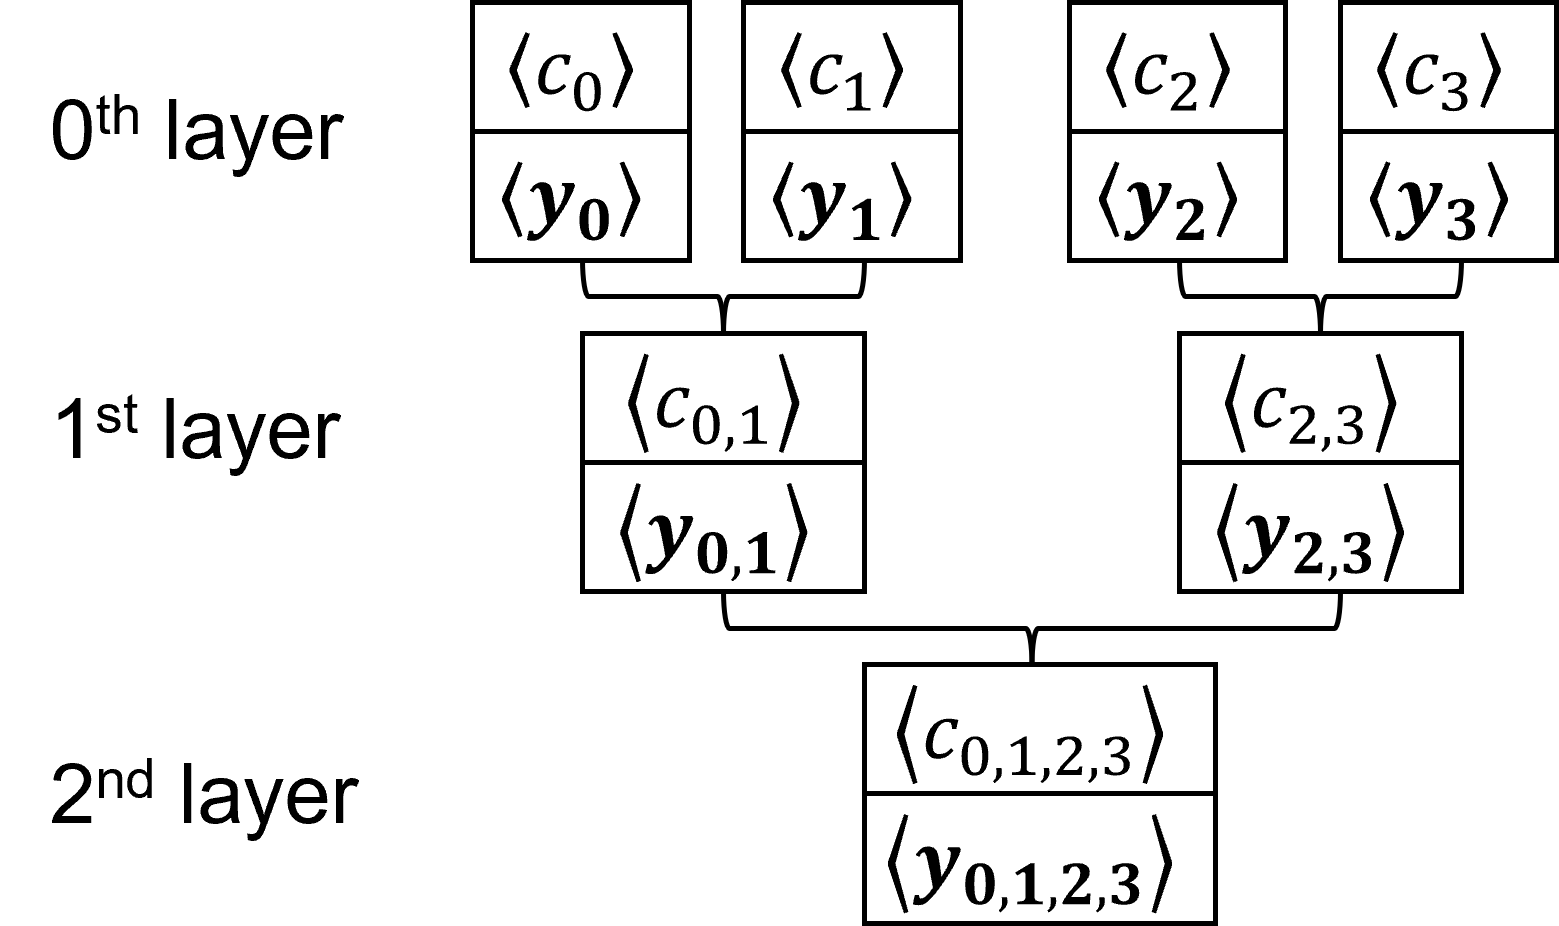
\includegraphics[width=10cm]{OAA_b.png}
%     \centering
%     \caption{Example inverted binary tree for $\Uppi^{OAA_b}$.}
%     \label{img:OAA_b}
% \end{figure}
% \FloatBarrier


% \subsection{Geometric Distribution}
% \label{prot:GeometricDistribution}
% \autoref{prot:Geometric} is constructed based on $Algo^{Geo}$ (cf.~\autoref{algo:Geometric}). 
% $ \left(u_0,\ldots,u_{iter} \right)\in \left\{0,1\right\}^{iter} $ is a bit string with uniform bits.
% In line $2,3$, we set the bits in $ b_0,\ldots,b_{iter-1}$ to one when the corresponding bits in $u_0,\ldots,u_{iter} $ are the leading zero bits, and other bits in $ b_0,\ldots,b_{iter-1}$ to zero. 
% Recall that the geometric distribution (cf.~\autoref{def:GeometricDistribution}) counts the number of Bernoulli trials up to and including the first success. Therefore, we append bit $1$ and compute the Hamming Weight of string $1, b_0,\ldots,b_{iter-1}$.

% \begin{protocol}[tbh!]
%     \centering
%     \fbox{
%         \pseudocode[space=none, syntaxhighlight=auto, addkeywords={Protocol, Input, Output,FOR,},linenumbering, skipfirstln, head=\textbf{Protocol: $\Uppi^{Geometric}$}]{
%             \textbf{Input: None} \pcskipln \\
%             \textbf{Output: $\left\langle \boldsymbol{y}\right\rangle^{B,UINT}$, where $y\sim Geo\left(p=0.5\right) $} \\
%             \text{$\left(u_0,\ldots,u_{iter-1}\right)  \gets \Uppi^{RandBits}\left(iter\right) $} \\
%             \text{$\left(\left\langle p_{0}\right\rangle^B,\ldots,\left\langle p_{iter-1}\right\rangle^B\right) =\Uppi^{PreOr}\left(\left\langle u_0\right\rangle^B,\ldots, \left\langle u_{iter-1}\right\rangle^B\right) $} \\
%             \text{$\left(\left\langle b_{0}\right\rangle^B,\ldots,\left\langle b_{iter-1}\right\rangle^B\right)  = \left(\operatorname{NOT} \left(\left\langle p_{0} \right\rangle ^B\right),\ldots,\operatorname{NOT} \left(\left\langle p_{iter-1} \right\rangle ^B\right) \right) $} \\
%             % \text{$\left(\left\langle z_0^{ind}\right\rangle^B,\dots,\left\langle z_{iter-1}^{ind}\right\rangle^B\right) =\left(1,\left\langle d_{0}\right\rangle ^B ,\ldots ,\left\langle d_{iter-2}\right\rangle ^B\right) $. }\\
%             \text{$\left\langle \boldsymbol{y}\right\rangle^{B,UINT} =\Uppi^{HW}\left(1,\left\langle b_{0}\right\rangle^B,\ldots,\left\langle b_{iter-2}\right\rangle^B\right) $.}
%         }}
%     \caption{MPC Protocol for geometric distribution $y\sim Geo\left(p=0.5\right)$.}
%     \label{prot:Geometric}
% \end{protocol}
% \FloatBarrier

% % \TODO{explanation}
% \TODO{anaylyse about differential privacy, $iter_2$ leak information of j in second while loop}\\
% \autoref{prot:GeometricExp} converts $Algo^{GeoExp}\left(n,d\right) $ (cf.~\autoref{algo:GeometricExp}) into MPC protocol for $n\neq 0$.
% % We assume two WHILE loop terinates in $iter_1$ and $iter_2$ loops.
% \begin{protocol}[tbh!]
%     \centering
%     \fbox{
%         \pseudocode[space=none, syntaxhighlight=auto, addkeywords={Protocol, Input, Output,FOR,TO},linenumbering, skipfirstln, head=\textbf{Protocol: $\Uppi^{GeometricExp}\left(n,d\right) $ }]{
%             \textbf{Input: $n$, $d$} \pcskipln \\
%             \textbf{Output: $\left\langle \boldsymbol{x}\right\rangle ^{B,UINT} $, where $x \sim Geo\left(p=1-e^{\frac{n}{d}}\right) $} \\
%             % first while loop
%             \text{FOR $j=0$ TO $ iter_1-1$}\\
%             \text{\t\t$\left\langle \boldsymbol{u_j}\right\rangle ^{B,UINT}\gets \Uppi^{RandInt}\left(d\right) $}\\
%             \text{\t\t$\left\langle \boldsymbol{\gamma_{1,j}}\right\rangle ^{B,FX}\gets \frac{\left\langle \boldsymbol{u_j}\right\rangle ^{B,UINT}}{d} $}\\
%             \text{\t\t$\left\langle b_{1,j}\right\rangle ^B=\Uppi^{BernoulliEXP1}\left(\left\langle \boldsymbol{\gamma_{1,j}}\right\rangle ^{B,FX}\right) $ }\\
%             % \text{$\left(\left\langle e_{1,0}\right\rangle ,\ldots,\left\langle e_{1,iter_1-1}\right\rangle \right) =\Uppi^{PreOr}\left(\left\langle b_{1,0}\right\rangle ^B,\ldots,\left\langle b_{1,iter-1}\right\rangle ^B\right) $}\\
%             % \text{For $j \in [1\ldots iter_1)$, parties compute $ \left\langle p^{1}_{j}\right\rangle ^B=\left\langle e^{1}_j\right\rangle^B-\left\langle e^{1}_{j-1}\right\rangle^B$, where $ \left\langle p^{1}_{0}\right\rangle ^B=\left\langle e^{1}_{0}\right\rangle ^B$ }\\
%             % \text{Parties calculate $\left\langle \boldsymbol{u}\right\rangle ^{B,UINT}=\sum_{j=0}^{iter_1-1} \left\langle p^{1}_{j}\right\rangle ^B*\left\langle \boldsymbol{u_j}\right\rangle ^{B,UINT} $}\\
%             % second while loop
%             \text{FOR $k=0$ TO $ iter_2-1$}\\
%             \text{\t\t$\left\langle b_{2,k}\right\rangle ^B=\Uppi^{BernoulliEXP1}\left(1\right) $}\\
%             % \text{$\left(\left\langle e^{2}_{0}\right\rangle ,\ldots,\left\langle e^{2}_{iter_1-1}\right\rangle \right) =\Uppi^{PreOr}\left(\text{NOT}\left(\left\langle b^{2}_{0}\right\rangle ^B\right) ,\ldots,\text{NOT}\left(\left\langle b^{2}_{iter-1}\right\rangle ^B\right) \right) $}\\
%             % \text{For $j \in [1\ldots iter_2)$, parties compute $ \left\langle p^{2}_{j}\right\rangle ^B=\left\langle e^{2}_j\right\rangle^B-\left\langle e^{2}_{j-1}\right\rangle^B$, where $ \left\langle p^{2}_{0}\right\rangle ^B=\left\langle e^{2}_{0}\right\rangle ^B$ }\\
%             % \text{Parties run $\left\langle \boldsymbol{k}\right\rangle ^{B,UINT} =\Uppi^{LeadingZeros}\left(\left\langle p^{2}_{0}\right\rangle ^B,\ldots,\left\langle p^{2}_{iter_2}\right\rangle ^B\right) $}\\
%             % final result
%             % \text{Parties calculate $\left\langle \boldsymbol{x}\right\rangle ^{B,UINT} =\text{FL2UI}\left(\text{Floor}\left(\text{DIV}\left(\text{ADD}\left(\text{MUL}\left(k,d\right), \left\langle \boldsymbol{u}\right\rangle ^{B,UINT}\right),n\right)\right)\right) $}
%             \text{$\left\langle \boldsymbol{u}\right\rangle^{B,UINT}\gets \Uppi^{ObliviousSelection}\left(\left\langle \boldsymbol{u_0}\right\rangle ^{B,UINT},\ldots,\left\langle \boldsymbol{u_{iter_1-1}}\right\rangle ^{B,UINT},\left\langle b_{1,0}\right\rangle ^B,\ldots,\left\langle b_{1,iter_1-1}\right\rangle ^B\right) $}\\
%             \text{$\left\langle \boldsymbol{k}\right\rangle^{B,UINT}\gets \Uppi^{ObliviousSelection}\left(0,\ldots,iter_2-1,\left\langle b_{2,0}\right\rangle ^B,\ldots,\left\langle b_{2,iter_2-1}\right\rangle ^B\right) $}\\
%             \text{$\left\langle \boldsymbol{x}\right\rangle ^{B,UINT}\gets \left\langle \boldsymbol{k}\right\rangle^{B,UINT} \cdot \frac{ d}{n}+\frac{\left\langle \boldsymbol{u}\right\rangle^{B,UINT}}{n}$}
%         }}
%     \caption{MPC Protocol for geometric distribution $x \sim Geo\left(p=1-e^{\frac{n}{d}}\right) $.}
%     \label{prot:GeometricExp}
% \end{protocol}
% \FloatBarrier



% \subsection{Bernoulli Distribution}
% \autoref{prot:Bernoulli} is based on~\autoref{algo:Bernoulli}.
% \begin{protocol}[tbh!]
%     \centering
%     \fbox{
%         \pseudocode[space=none, syntaxhighlight=auto, addkeywords={Protocol, Input, Output},linenumbering, skipfirstln, head=\textbf{Protocol: $\Uppi^{Bernoulli}\left(\left\langle \boldsymbol{p}\right\rangle ^{B,FX} \right) $ }]{
%             \textbf{Input: $\left\langle \boldsymbol{p}\right\rangle ^{B,FX}$} \pcskipln \\
%             \textbf{Output: $\left\langle x\right\rangle ^{B} $, where $x\sim Bern\left(p\right) $} \\
%             \text{$\left\langle \boldsymbol{U}\right\rangle ^{B,UINT} \gets \Uppi^{RandBits}\left(11\right) $}\\
%             \text{$\left\langle \boldsymbol{U}\right\rangle ^{B,FX} \gets \operatorname{UI2FP}\left(\left\langle \boldsymbol{U}\right\rangle ^{B,UINT}\right)  $}\\
%             \text{$\left\langle \boldsymbol{U}\right\rangle ^{B,FX} \gets \operatorname{right-shift}\left(\left\langle \boldsymbol{U}\right\rangle ^{B,FX} ,11\right)  $}\\
%             \text{$\left\langle x\right\rangle^{B} \gets \left(\left\langle p\right\rangle^{B,FX} >\left\langle \boldsymbol{U}\right\rangle ^{B,FX}\right) $}
%         }}
%     \caption{MPC Protocol for Bernoulli distribution $x\sim Bern\left(p\right) $.}
%     \label{prot:Bernoulli}
% \end{protocol}
% \FloatBarrier

% \autoref{prot:BernoulliEXP1} convert $Algo^{BernEXP1}\left(\gamma\right) $~\cite{canonne2020discrete} into MPC protocols. 
% \begin{protocol}[tbh!]
%     \centering
%     \fbox{
%         \pseudocode[space=none, syntaxhighlight=auto, addkeywords={Protocol, Input, Output,FOR},linenumbering, skipfirstln, head=\textbf{Protocol: $\Uppi^{BernoulliEXP1}\left(\left\langle \boldsymbol{\gamma}\right\rangle ^{B,FX}\right) $ }]{
%             \textbf{Input: $\left\langle \boldsymbol{\gamma}\right\rangle ^{B,FX}$} \pcskipln \\
%             \textbf{Output: $\left\langle x\right\rangle ^{B} $, where $x\sim Bern\left(p=e^{-\gamma}\right) $ and $\gamma \in \left[0,1\right] $} \\
%             \text{FOR $j \in [1\ldots iter]$}\\
%             \text{\t\t$\left\langle \boldsymbol{p_j}\right\rangle ^{B,FX}\gets  \frac{\left\langle \boldsymbol{\gamma}\right\rangle ^{B,FX}}{j}  $}\\
%             \text{\t\t$\left\langle b_j\right\rangle ^{B}\gets \Uppi^{Bernoulli}\left(\left\langle \boldsymbol{p_j}\right\rangle ^{B,FX}\right) $}\\
%             \text{\t\t$\left\langle fg_j\right\rangle^{B} \gets \left(\left\langle b_j\right\rangle ^{B}==1\right) $}\\
%             % \text{Parties run $\left(\left\langle e_0\right\rangle^{B} ,\ldots, \left\langle e_{iter}\right\rangle^{B}\right) =\Uppi^{PreOr}\left(\left\langle fg_0\right\rangle^{B},\ldots,\left\langle fg_{iter}\right\rangle^{B}\right) $}\\
%             % \text{For $j \in [1\ldots iter)$, parties compute $ \left\langle p_{j}\right\rangle ^B=\left\langle e_j\right\rangle^B-\left\langle e_{j-1}\right\rangle^B$, where $ \left\langle p_{0}\right\rangle ^B=\left\langle e_{0}\right\rangle ^B$ }\\
%             % \text{Parties compute $\left\langle x \right\rangle^B=\sum_{j = 0}^{iter-1} \left\langle p_{j}\right\rangle ^B*\left\langle b_j\right\rangle ^{B}$}
%             \text{$\left\langle x \right\rangle^B\gets \Uppi^{ObliviousSelection}\left(j_{mod2},\left\langle fg_1\right\rangle^{B},\ldots,\left\langle fg_{iter}\right\rangle^{B}\right) $, where $j_{mod2}=\left(1,0,1,0,\ldots\right) $}
%         }}
%     \caption{MPC Protocol for Bernoulli distribution $x\sim Bern\left(p=e^{-\gamma}\right) $, where $\gamma \in \left[0,1\right] $.}
%     \label{prot:BernoulliEXP1}
% \end{protocol}
% \FloatBarrier


% \autoref{prot:BernoulliEXP} converts $Algo^{BernEXP}\left(\gamma\right) $~\cite{canonne2020discrete} into MPC protocol.
% % We assume that $\gamma<iter$.
% % In line $1,2$, the parties calculate the condition and Bernoulli sampling for the first case.
% % In line $3-13$, the parties calcualte the conditiaon and Bernoulli sampling for the second case. In line $6-8$, the parties extract $b_2==0$ which terminates the for loop under $iter$ iterations. In line $9-12$, the parties calculate the index $j$ where the for loops terminates and compare it with $\left\lfloor \gamma\right\rfloor $ as the condition for case 2.
% % In line $14$, the parties calculate the Bernoulli samples under third case.
% % Finally, the parties calcualte $\left\langle x\right\rangle ^{B} =\left\langle cond_{\gamma \in \left[0,1\right] }\right\rangle ^B*\left\langle b_1\right\rangle ^B+\text{NOT}\left(\left\langle cond_{\gamma \in \left[0,1\right] }\right\rangle ^B\right) *\left(\left\langle cond_{ b2}\right\rangle ^B *\left\langle b_2\right\rangle ^B+\text{NOT}\left(\left\langle cond_{ b2}\right\rangle ^B\right) *\left\langle b_{3}\right\rangle ^B\right) $.

% % Note that the assumption $\gamma<iter$ reveals information about $\gamma$, which implies weaker differential privacy strength.
% % \TODO{anaylyse about differential privacy}\\
% % set the $flag$ to record if the $b_j=1$ is satisfied. In line $5, 6$, the parties calculate the position $p_0,\ldots,p_{iter-1}$ where $p_j=1$ and $j$ is the smallest number such that $flag_j=1$, i.e., the $\text{WHILE}$ loop conditionis not satisfied and algorithms return a result $x=b_j$.\\

% Note that in line $10$, the parties compute $\left\langle x\right\rangle ^B$ with $\left\langle \boldsymbol{b}\right\rangle ^B=\left(\left\langle b_1\right\rangle^B,\left\langle b_{2,0}\right\rangle ^B,\ldots,\left\langle b_{2,iter-1}\right\rangle ^B,\left\langle b_3\right\rangle^B\right) $ and $\left\langle \boldsymbol{fg}     \right\rangle ^{B} =\left(\left\langle cond_{b1}\right\rangle ^B,\left\langle cond_{ b2,0}\right\rangle ^B,\ldots,\left\langle cond_{ b2,iter-1}\right\rangle ^B,1\right)$.


% \begin{protocol}[tbh!]
%     \centering
%     \fbox{
%         \pseudocode[space=none, syntaxhighlight=auto, addkeywords={Protocol, Input, Output,FOR,TO},linenumbering, skipfirstln, head=\textbf{Protocol: $\Uppi^{BernoulliEXP}\left(\left\langle \boldsymbol{\gamma}\right\rangle ^{B,FX}\right) $ }]{
%             \textbf{Input: $\left\langle \boldsymbol{\gamma}\right\rangle ^{B,FX}$} \pcskipln \\
%             \textbf{Output: $\left\langle x\right\rangle ^{B} $, where $x\sim Bern\left(p=e^{-\gamma}\right) $} \\
%             % \gamma \in \left[0,1\right] 
%             % b_1
%             \text{$\left\langle cond_{b1}\right\rangle ^B\gets  \left(\left\langle \boldsymbol{\gamma}\right\rangle ^{B,FX}\leq1\right)   $}\\
%             \text{$\left\langle b_1\right\rangle ^B\gets \Uppi^{BernoulliEXP1}\left(\left\langle \boldsymbol{\gamma}\right\rangle ^{B,FX}\right) $}\\
%             % \gamma >1
%             % b_2
%             \text{$\left\langle \boldsymbol{\left\lfloor \gamma\right\rfloor }\right\rangle ^{B,FX}\gets \operatorname{Floor}\left(\left\langle \boldsymbol{\gamma}\right\rangle ^{B,FX}\right) $}\\
%             \text{FOR $j=0$ TO $ iter-1 $}\\
%             \text{\t\t$\left\langle b_{2,j}\right\rangle ^B \gets \Uppi^{BernoulliEXP1}\left(1\right) $}\\
%             \text{\t\t$\left\langle cond_{b_{2,j}==0}\right\rangle ^B \gets \left(\left\langle b_{2,j}\right\rangle ^B ==0\right) $}\\
%             % \text{$\left(\left\langle e_{0}\right\rangle ,\ldots,\left\langle e_{iter-1}\right\rangle \right) =\Uppi^{PreOr}\left(\left\langle b_{0,2}\right\rangle ^B,\ldots,\left\langle b_{iter-1,2}\right\rangle ^B\right) $}\\
%             % \text{For $j \in [1\ldots iter)$, parties compute $ \left\langle p_{j}\right\rangle ^B=\left\langle e_j\right\rangle^B-\left\langle e_{j-1}\right\rangle^B$, where $ \left\langle p_{0}\right\rangle ^B=\left\langle e_{0}\right\rangle ^B$ }\\
%             % \text{Parties calculate $\left\langle b_2\right\rangle ^B=\sum_{j=0}^{iter-1} \left\langle p_{j}\right\rangle ^B*\left\langle b_{j,2}\right\rangle ^B $}\\
%             % \text{Parties calculate $\left\langle \boldsymbol{j_{b_{j,2}==0}}\right\rangle ^{B,UINT}=\Uppi^{LeadingZeros}\left(\left\langle p_{0}\right\rangle ^B,\ldots,\left\langle p_{iter-1}\right\rangle ^B\right) $}\\
%             % \text{Parties calcualte $\left\langle \boldsymbol{\left\lfloor \gamma\right\rfloor }\right\rangle ^{B,UINT}=\text{FL2UI}\left(\left\langle \boldsymbol{\left\lfloor \gamma\right\rfloor }\right\rangle ^{B,FL}\right) $}\\
%             \text{\t\t$\left\langle cond_{ b2,j}\right\rangle ^B \gets \left(j< \left\langle \boldsymbol{\left\lfloor \gamma\right\rfloor }\right\rangle ^{B,FX}\right)  \land \left\langle cond_{b_{2,j}==0}\right\rangle ^B  $}\\
%             % b_3
%             \text{$\left\langle \boldsymbol{\gamma-\left\lfloor \gamma\right\rfloor }\right\rangle ^{B,FX}\gets \left\langle \boldsymbol{\gamma}\right\rangle ^{B,FX} -\left\langle \boldsymbol{\left\lfloor \gamma\right\rfloor }\right\rangle ^{B,FX}$}\\
%             \text{$\left\langle b_{3}\right\rangle ^B =\Uppi^{BernoulliEXP1}\left(\left\langle \boldsymbol{\gamma-\left\lfloor \gamma\right\rfloor }\right\rangle ^{B,FL}\right) $}\\
%             % final result
%             \text{$ \left\langle x\right\rangle ^{B} \gets \Uppi^{ObliviousSelection}\left(\left\langle \boldsymbol{b}\right\rangle ^B, \left\langle \boldsymbol{fg}     \right\rangle ^{B}   \right) $}
%         }}
%     \caption{MPC Protocol for Bernoulli distribution $x\sim Bern\left(p=e^{-\gamma}\right) $.}
%     \label{prot:BernoulliEXP}
% \end{protocol}
% \FloatBarrier

% \subsection{Random Integer}
% \autoref{prot:RandInt} convert $Algo^{RandInt}\left(m\right)$ into MPC protocol.\\
% \TODO{Problem with unsigned integer because $\kappa$ is requires be greater than 64.}\\
% \begin{protocol}[tbh!]
%     \centering
%     \fbox{
%     \pseudocode[space=none, syntaxhighlight=auto, addkeywords={Protocol, Input, Output},linenumbering, skipfirstln, head=\textbf{Protocol: $\Uppi^{RandInt}\left(m\right) $ }]{
%     \textbf{Input: $m$} \pcskipln \\
%     \textbf{Output: $\left\langle \boldsymbol{x}\right\rangle ^{B,UINT} $, where $x \in [0,m) $} \\
%     \text{$\left\langle \boldsymbol{r}\right\rangle ^{B,UINT} \gets \Uppi^{RandBits}\left(l+kappa\right)$ }\\
%     \text{$\left\langle \boldsymbol{x}\right\rangle^{B,UINT} \gets \text{MOD}\left(\left\langle \boldsymbol{r}\right\rangle ^{B,UINT},m\right) $}
%     }}
%     \caption{MPC Protocol for random integer $x \sample [0,m) $.}
%     \label{prot:RandInt}
% \end{protocol}
% \FloatBarrier








% % Protocol $\Uppi^{LeadingZeros}\left(\left\langle \boldsymbol{s} \right\rangle^B,l\right) $ counts the number of leading zeros in a $l$-bit string $\boldsymbol{s}$. We apply $\Uppi^{PreOr} $ to find the position $e$ of the first appearance of one in string $\boldsymbol{s}$. Finally, by inverting $e$, we get $e_j=1$ if $s_j$ belongs to the leading zeros. In line $3$, we convert boolean share to arithmetic share to count the total number of leading zeros (number of $d_j\neq 0$).\\
% % \begin{protocol}[tbh!]
% %     \centering
% %     \fbox{
% %     \pseudocode[space=none, syntaxhighlight=auto, addkeywords={Protocol, Input, Output},linenumbering, skipfirstln, head=\textbf{Protocol: $\Uppi^{LeadingZeros}\left(\left\langle \boldsymbol{s}\right\rangle^B,l\right) $}]{
% %     \textbf{Input: $l$-bit string $\left\langle \boldsymbol{s}\right\rangle^B$ } \pcskipln \\
% %     \textbf{Output: $\left\langle z\right\rangle^A$} \\
% %     \text{Parties run $\Uppi^{PreOr}\left(\left\langle \boldsymbol{s} \right\rangle^B\right) $ and obtain $\left\langle e_{j}\right\rangle^B$. } \\
% %     \text{For $j \in [0\ldots l)$, parties compute $\left\langle d_j\right\rangle^B=\text{NOT}\left(\left\langle e_{j}\right\rangle^B\right) in parallel$. }\\
% %     \text{Parties compute $\left\langle \boldsymbol{z}\right\rangle^{B,UINT}=\sum_{j = 0}^{l-1}\text{B2A}\left(\left\langle d_{j}\right\rangle^B \right) $. }
% %     }}
% %     \caption{MPC Protocol for counting leading zeros.}
% %     \label{prot:LeadingZeros}
% % \end{protocol}
% % \FloatBarrier

% % Protocol $\Uppi^{BitsContainOne}\left(\left\langle \boldsymbol{s} \right\rangle^B,l\right) $ outputs $o=1$ if the given $l$-bit string $\boldsymbol{s}$ contains one, and $o=0$ otherwise.\\
% % \begin{protocol}[tbh!]
% %     \centering
% %     \fbox{
% %         \pseudocode[space=none, syntaxhighlight=auto, addkeywords={Protocol, Input, Output},linenumbering, skipfirstln, head=\textbf{Protocol: $\Uppi^{BitsContainOne}$}]{
% %             \textbf{Input: $l$-bit string $\left\langle \boldsymbol{s}\right\rangle^B$ } \pcskipln \\
% %             \textbf{Output: $\left\langle o\right\rangle^B$} \\
% %             \text{Parties compute $\left\langle o\right\rangle ^B=\lor _{j=0}^{l}\left\langle s_{j}\right\rangle^B$ }
% %         }}
% %     \caption{MPC Protocol for checking if $l$-bit string $s$ contains one.}
% %     \label{prot:BitsContainOne}
% % \end{protocol}
% % \FloatBarrier

% \subsection{Binary2Unary}

% \TODO{Binary2Unary needs to be improved.}
% $\Uppi^{Binary2Unary}\left(\left\langle a\right\rangle^A ,l\right) $~\cite{aliasgari2012secure} converts integer $a$ from binary to unary bitwise representation and outputs a $l$-bit string $\boldsymbol{p}=\left( p_{0} ,\ldots , p_{l-1} \right) $, where the $a$ least significant bits $\left( p_{0} ,\ldots , p_{a-1} \right)$ are set to $1$ and others to $0$. In line $1,2$, we calculate the $2^a$ and convert it to boolean shares. Then in line $3$ we generate $l+k$ random bits and hide $2_a$ by adding it with the $l+k-1$-bit integer and reconstruct the addition result $c$. In line $5$, the plaintext value $c$ is decomposed into binary bits. In line $6$, we compute $XOR$ of $c_j$ and correspond bit $u_j$. Then in line $7$, by $PreOr$ we get $\left(g_{l-1},\ldots,g_j\right) =\left(\overline{1}_{\left(l-j+1\right) }\right) $ and $\left(g_{j-1},\ldots,g_{0}\right) =\left(\overline{0}_{\left(j\right) }\right) $, where $j-1=a$. Finally, we calculate $\left(p_{l-1},\ldots,p_{0}\right)=\text{NOT}\left(g_{l-1},\ldots,g_{0}\right) $ and the number of non-zero bits in $\left(p_{l-1},\ldots,p_{0}\right)$ equals to $a$. The share conversion in line $4$ can be omitted if arithmetic of boolean shares is available.\\
% \begin{protocol}[tbh!]
%     \centering
%     \fbox{
%     \pseudocode[space=none, syntaxhighlight=auto, addkeywords={Protocol, Input, Output},linenumbering, skipfirstln, head=\textbf{Protocol: $\Uppi^{Binary2UnaryOld}\left(\left\langle a\right\rangle^A ,l\right) $}]{
%     \textbf{Input: $\left\langle \boldsymbol{a}\right\rangle^B $, $l$} \pcskipln \\
%     \textbf{Output: $\left\langle p_{0}\right\rangle ^B,\ldots ,\left\langle p_{l-1}\right\rangle^B $} \\
%     \text{Parties compute $\left\langle \boldsymbol{2^{a}}\right\rangle ^B=\text{Pow2}\left(\left\langle a\right\rangle ^A,l\right) $} \\
%     \text{Parties compute $ \left\langle 2^{a}\right\rangle ^A=\text{B2A}\left(\left\langle \boldsymbol{2^{a}} \right\rangle ^B\right) $} \\
%     \text{Parties run $\Uppi^{RandBits}\left(l+k\right) $ and obtain $\left\langle u_0\right\rangle ^B,\ldots,\left\langle u_{l+k-1}\right\rangle ^B$.} \\
%     % \text{Parties reconstruct $c \gets \text{Rec}\left(\left\langle 2^{a}\right\rangle^A+2^{l}*\text{B2A}\left(\left\langle u_{l+k-1}\right\rangle ^B,\ldots, \left\langle u_l\right\rangle ^B\right) + \text{B2A}\left(\left\langle u_{l-1}\right\rangle^B,\ldots,\left\langle u_0\right\rangle^B \right) \right) $} \\
%     \text{Parties reconstruct $c \gets \text{Rec}\left(\left\langle 2^{a}\right\rangle^A + \text{B2A}\left(\left\langle u_{l+k-1}\right\rangle^B,\ldots,\left\langle u_0\right\rangle^B \right) \right) $} \\
%     \text{Each party locally run $\Uppi^{Bits}\left(c,l\right) $ and obtain $\left(c_{0},\ldots ,c_{l-1}\right) $} \\
%     \text{For $j\in\left[0 \ldots l\right) $, each party locally compute $\left\langle t_j\right\rangle^B =\text{XOR}\left(c_j,\left\langle u_j\right\rangle ^B\right) $} \\
%     \text{For $j\in\left[0 \ldots l\right) $, parties compute $\Uppi^{PreOr}\left(\left\langle t_0\right\rangle^B,\ldots, \left\langle t_l\right\rangle^B\right) $ and obtain $\left\langle g_0\right\rangle^B,\ldots, \left\langle g_l\right\rangle^B$}\\
%     \text{For $j\in\left[0 \ldots l\right) $, parties compute $\left\langle p_j\right\rangle^B =\text{NOT}\left(\left\langle g_j\right\rangle ^B\right) $}
%     }}
%     \caption{MPC Protocol for binary to unary conversion.}
%     \label{prot:Binary2Unary}
% \end{protocol}
% \FloatBarrier

% \begin{protocol}[tbh!]
%     \centering
%     \fbox{
%         \pseudocode[space=none, syntaxhighlight=auto, addkeywords={Protocol, Input, Output},linenumbering, skipfirstln, head=\textbf{Protocol: $\Uppi^{Binary2UnaryNEW}\left(\left\langle \boldsymbol{a}\right\rangle^{B,UINT} ,l\right) $}]{
%             \textbf{Input: $\left\langle \boldsymbol{a}\right\rangle^{B,UINT} $, $l$} \pcskipln \\
%             \textbf{Output: $\left\langle p_{0}\right\rangle ^B,\ldots ,\left\langle p_{l-1}\right\rangle^B $} \\
%             \text{Parties compute $\left\langle \boldsymbol{t}\right\rangle ^{B,UINT}=\text{POW2}\left(\left\langle \boldsymbol{a}\right\rangle ^{B,UINT}\right) $.} \\
%             \text{Parties compute $\left(\left\langle e_0\right\rangle^B,\ldots,\left\langle e_{64-1}\right\rangle^B\right) =\Uppi^{PreOr}\left(\left\langle t_0\right\rangle^B,\ldots,\left\langle t_{64-1}\right\rangle^B\right) $.} \\
%             \text{Each party locally set $\left\langle p_0\right\rangle^B=\text{NOT}\left(\left\langle e_0\right\rangle^B\right) ,\ldots,\left\langle p_{l-1}\right\rangle^B=\text{NOT}\left(\left\langle e_{l-1}\right\rangle^B\right) $.}
%         }}
%     \caption{MPC Protocol for binary to unary conversion.}
%     \label{prot:Binary2Unary}
% \end{protocol}
% \FloatBarrier




% % \begin{protocol}[tbh!]
% %     \centering
% %     \fbox{
% %         \pseudocode[space=none, syntaxhighlight=auto, addkeywords={Protocol, Input, Output},linenumbering, skipfirstln, head=\textbf{Protocol: $\Uppi^{Split}\left(\left\langle \boldsymbol{L}\right\rangle^{B,UINT} ,\left\langle \boldsymbol{R}\right\rangle ^{B,UINT} ,\lambda\right) $}]{
% %             \textbf{Input: $\left\langle \boldsymbol{L}\right\rangle^{B,UINT}$, $\left\langle \boldsymbol{R}\right\rangle ^{B,UINT}$, $\lambda$} \pcskipln \\
% %             \textbf{Output: $\left\langle \boldsymbol{M}\right\rangle^{B,UINT}$, where $M=L-\text{int}\left(\frac{\ln\left(0.5\right)+\ln\left(1+e^{-\lambda\left(R-L\right) }\right) }{\lambda}\right)$} \\
% %             \text{Parties compute $\left\langle \boldsymbol{t}\right\rangle ^{B,FL}=\frac{\text{LN}\left(0.5\right)+\text{LN}\left(1+\text{EXP}\left(-\lambda \cdot \left(\left\langle \boldsymbol{R}\right\rangle ^{B,UINT}-\left\langle \boldsymbol{L}\right\rangle^{B,UINT}\right)\right) \right) }{\lambda}$.}\\
% %             \text{Parties compute $\left\langle \boldsymbol{M}\right\rangle^{B,UINT}=\left\langle \boldsymbol{L}\right\rangle^{B,UINT}-\text{FL2UI}\left(\left\langle \boldsymbol{t}\right\rangle ^{B,FL}\right) $.}
% %         }}
% %     \caption{MPC Protocol for $\text{Split}\left(L,R,\lambda\right)=L-\text{int}\left(\frac{\ln\left(0.5\right)+\ln\left(1+e^{-\lambda\left(R-L\right) }\right) }{\lambda}\right) $.}
% %     \label{prot:Split}
% % \end{protocol}
% % \FloatBarrier

% % \begin{protocol}[tbh!]
% %     \centering
% %     \fbox{
% %         \pseudocode[space=none, syntaxhighlight=auto, addkeywords={Protocol, Input, Output},linenumbering, skipfirstln, head=\textbf{Protocol: $\Uppi^{Proportion}\left(\left\langle \boldsymbol{L_{j-1}}\right\rangle^{B,UINT} ,\left\langle \boldsymbol{R_{j-1}}\right\rangle ^{B,UINT} ,\left\langle \boldsymbol{M_j}\right\rangle ^{B,UINT} ,\lambda\right)$}]{
% %             \textbf{Input: $\left\langle \boldsymbol{L}\right\rangle^{B,UINT}$, $\left\langle \boldsymbol{R}\right\rangle ^{B,UINT}$, $\left\langle \boldsymbol{M}\right\rangle^{B,UINT}$, $\lambda$} \pcskipln \\
% %             \textbf{Output: $\left\langle \boldsymbol{Q}\right\rangle ^{B,FL}$, where $Q=\frac{e^{-\lambda\left(M-L\right) }-1}{e^{-\lambda\left(R-L\right) }-1} $} \\
% %             \text{Parties compute $\left\langle \boldsymbol{Q}\right\rangle ^{B,FL}=\frac{e^{-\lambda \cdot \left(\left\langle \boldsymbol{M}\right\rangle ^{B,FL}-\left\langle \boldsymbol {L}\right\rangle ^{B,FL}\right) }-1}{e^{-\lambda \cdot \left(\left\langle \boldsymbol{R}\right\rangle ^{B,FL}- \left\langle \boldsymbol{L}\right\rangle ^{B,FL}\right) }-1} $.}
% %         }}
% %     \caption{MPC Protocol for $\text{Proportion}\left(L,R,M,\lambda\right)=\frac{e^{-\lambda\left(M-L\right) }-1}{e^{-\lambda\left(R-L\right) }-1} $.}
% %     \label{prot:Proportion}
% % \end{protocol}
% % \FloatBarrier





% % \begin{algorithm}[tbh!]
% %     \centering
% %     \fbox{
% %     \pseudocode[space=none, syntaxhighlight=auto, addkeywords={Protocol, Input, Output},linenumbering, head=\textbf{Function $\text{AGT}\left(\left\langle x_0\right\rangle^A, \left\langle x_1\right\rangle^A,\ell_s \right)  $}]{
% %     \text{$\left\langle \delta \right\rangle^A=\left\langle x_1\right\rangle^A-\left\langle x_0\right\rangle^A $}\\
% %     \text{$\ell_{prev}=1$}\\
% %     \text{if $\ell>\ell_s$ then}\\
% %     \text{\t\t if $\ell==\ell_s+2$ then}\\
% %     \text{\t\t \t\t $\ell_s=\ell_s+1$}\\
% %     \text{\t\t $sel \gets\left\langle \delta \right\rangle^A_0\left[1:\ell_s\right] $ }\\
% %     \text{\t\t     $M  \gets\left(j+\langle\delta\rangle_{1}^{A}\left[1: \ell_{s}\right]>2^{\ell_{s}}\right)_{j=1}^{2^{\ell_s}} $ }\\
% %     \text{\t\t $r  \sample \left\{0,1\right\} $}\\
% %     \text{\t\t $c\gets \binom{N}{1} \text{-OT}\left(sel,\left\{m\oplus r\right\}_{m\in M} \right) $}\\
% %     \text{\t\t $\ell_{prev}\gets \ell_s+1$}\\
% %     \text{while $\ell_{prev} < \ell-1$}\\
% %     \text{\t\t $\ell_{s}^{\prime} \gets \min \left(\ell_{s}-1, \ell-\ell_{prev }-1\right)$}\\
% %     \text{\t\t $\ell_ {next }\gets \ell_ {prev }+\ell_{s}^{\prime}$}\\
% %     \text{\t\t if $\ell_{next}+2==\ell$ then}\\
% %     \text{\t\t \t\t $\ell_{next}=\ell_{next}+1$}\\
% %     \text{\t\t $ sel \gets \left\langle \delta\right\rangle_{0} ^{A}  \left[\ell_{prev}: \ell_{next }\right] .$}\\
% %     \text{\t\t $sel\gets sel+c\cdot 2^{\ell_s^{\prime}+1}$}\\
% %     \text{\t\t $\left\langle\delta^{\prime}\right\rangle_{1}^{A} \gets\langle\delta\rangle_{1}^{A}\left[\ell_{prev }: \ell_{next }\right]$}\\
% %     \text{\t\t $M_{0} \gets\left\{j+\left\langle\delta^{\prime}\right\rangle_{1}^{A}>2^{\ell_{s}^{\prime}+1}\right\}_{j=1}^{2^{\ell_s^{\prime}+1}}$}\\
% %     \text{\t\t $M_{1} \gets\left\{j+\left\langle\delta^{\prime}\right\rangle_{1}^{A}+1>2^{\ell_{s}^{\prime}+1}\right\}_{j=1}^{2^{\ell_s^{\prime}+1}}$}\\
% %     \text{\t\t $M \gets M_{r} \cup M_{1-r}$}\\
% %     \text{\t\t $r \sample \left\{0,1\right\} $}\\
% %     \text{\t\t $c\gets \binom{N}{1} \text{-OT}\left(sel,\left\{m\oplus r\right\}_{m\in M} \right) $}\\
% %     \text{\t\t $\ell_{prev } \gets \ell_{next }+1$}\\
% %     \text{$\left\langle b\right\rangle^B=\left(\left\langle b\right\rangle_0^B, \left\langle b\right\rangle_1^B\right):=\left(c\oplus \left\langle \delta \right\rangle^A_0\left[\ell\right]  ,r\oplus\left\langle \delta \right\rangle^A_1\left[\ell\right] \right)  $}\\
% %     \text{return $\left\langle b\right\rangle^B $}
% %     }}
% % \end{algorithm}
% % \FloatBarrier


% % \section{MPC Techniques}
% % \label{sec:MPCTechniques}
% % We applied certain techniques to convert algorithms into computations of MPC.

% % \subsection{Branching}
% % We convert \textbf{IF} branching in algorithm $Algo^{Branching}$~\autoref{algo:Branching} into MPC computations as

% % \[\text{output}=\left\langle a\right\rangle^B \land \left\langle b\right\rangle ^B \oplus  \text{NOT}\left(\left\langle a\right\rangle ^B\right) \land \left\langle c\right\rangle^B . \]

% % \begin{algorithm}[tbh!]
% %     \centering
% %     \fbox{
% %         \pseudocode[space=none, syntaxhighlight=auto, addkeywords={Protocol, Input, Output, IF, ELSE, RETURN},linenumbering, skipfirstln, head=\textbf{Protocol: $Algo^{Branching}$}]{
% %             % \textbf{Input: $\left\langle e\right\rangle^A $} \pcskipln \\
% %             % \textbf{Output: $\left( \left\langle y_{1}\right\rangle ^B, \ldots, \left\langle y_{11} \right\rangle ^B \right)$, $\left\langle y\right\rangle ^A$} \\
% %             \text{$\ldots$} \\
% %             \text{IF $\left\langle a\right\rangle^B $ }\\
% %             \text{\t\t RETURN $\left\langle b\right\rangle^B $}\\
% %             \text{ELSE}\\
% %             \text{\t\t RETURN $\left\langle c\right\rangle ^B$}\pcskipln\\
% %             \text{$\ldots$}
% %         }}
% %     \caption{Algorithm example with \textbf{IF} branching.}
% %     \label{algo:Branching}
% % \end{algorithm}
% % \FloatBarrier


% % \subsection{Loop}
% % Suppose $Algo^{Lottery}$~\autoref{algo:Lottery} is a lottery algorithm (charging $b$ amount of money for each draw) that you can draw unlimited times , and the reward $r$ decreases as the number of draws increases. $Algo^{Toss}$ output either $1$ (win) or $0$ (lose) with the same probability $p=0.5$.

% % \begin{algorithm}[tbh!]
% %     \centering
% %     \fbox{
% %         \pseudocode[space=none, syntaxhighlight=auto, addkeywords={Protocol, Input, Output, IF, ELSE, RETURN, WHILE, TRUE},linenumbering, skipfirstln, head=\textbf{Algorithm: $Algo^{Lottery}$}]{
% %             \text{$\ldots$} \\
% %             \text{$trials\gets 0$}\\
% %             \text{WHILE TRUE }\\
% %             \text{\t\t $  a \gets Algo^{Toss}\left(  b \right) $}\\
% %             \text{\t\t IF $a$}\\
% %             \text{\t\t \t\t RETURN $r-trials$}\\
% %             \text{\t\t $trials\gets trials+1$} \pcskipln \\
% %             \text{$\ldots$}
% %         }}
% %     \caption{Algorithm example with \textbf{WHILE} loop.}
% %     \label{algo:Lottery}
% % \end{algorithm}
% % \FloatBarrier

% % To transform $Algo^{Lottery}$ into MPC computations, the parties first assume that they will get the reward (i.e., \textbf{WHILE} loop terminates when $\left\langle a_j\right\rangle^{B}==1 $ for the first time) after $iter$ trials with very high probability. Then, the parties run $\Uppi^{Toss}$ for $iter$ times to compute $\left\langle a_j\right\rangle^{B} $ for $j \in [0\ldots iter)$. Since they don't know when $\left\langle a_j\right\rangle^{B}==1 $ happens for the first time, they run $\Uppi^{PreOr}$ in line $4$ to calculate $e_j=\lor_{k=0}^{j}a_{k}$ such that $e_0=0,\ldots,e_{s-1}=0$ and $e_s=1,\ldots,e_{iter-1}=1$, where $s$ is the smallest index in interval $ [0\ldots iter)$ making $\left\langle a_j\right\rangle^{B}==1 $. In line $6$, they calculate and get $p_s=1$, $p_t=0$ for $t \in [0\ldots iter)\setminus s$. Finally, the parties $\text{AND}$ the reward of each iteration with $p_j$ for $j \in [0\ldots iter)$ and $\text{XOR}$ these values to extract the correct reward $x$.

% %             \begin{protocol}[tbh!]
% %                 \centering
% %                 \fbox{
% %                     \pseudocode[space=none, syntaxhighlight=auto, addkeywords={Protocol, Input, Output, IF, ELSE, RETURN, WHILE, TRUE, FOR, TO},linenumbering, skipfirstln, head=\textbf{Protocol: $\Uppi^{Lottery}$}]{
% %                         \text{$\ldots$} \\
% %                         \text{Each party locally set $trial=0$.}\\
% %                         \text{FOR $j=0$ TO $iter-1$ }\\
% %                         \text{\t\t Parties run $\left\langle a_j\right\rangle^{B}= \Uppi^{Toss}\left(\left\langle \boldsymbol{b}\right\rangle^{B,UINT }\right) $.}\\
% %                         \text{Parties compute $\left(\left\langle e_0\right\rangle^B,\ldots,\left\langle e_{iter-1}\right\rangle^B\right) =\Uppi^{PreOr}\left(\left\langle a_0\right\rangle^B,\ldots,\left\langle a_{iter-1}\right\rangle^B\right) $.}\\
% %                         \text{FOR $j=0$ TO $iter-1$ }\\
% %                         \text{\t\t Each party locally compute $ \left\langle p_{j}\right\rangle ^B=\left\langle e_j\right\rangle^B \oplus \left\langle e_{j-1}\right\rangle^B$, where $ \left\langle p_{0}\right\rangle ^B=\left\langle e_{0}\right\rangle ^B$.} \\
% %                         \text{Parties compute $\left\langle x\right\rangle^{B,UINT}=\oplus_{j=0}^{iter-1}\left\langle p_{j}\right\rangle ^B \land \left(\left\langle \boldsymbol{r}\right\rangle^{B,UINT}-j\right) $.}\pcskipln \\
% %                         \text{$\ldots$}
% %                     }}
% %                 \caption{MPC protocol for algorithm with \textbf{WHILE} loop.}
% %                 \label{prot:Lottery}
% %             \end{protocol}
% %             \FloatBarrier





% \section{Additional Proof}
% \label{sec:additionalProof}

% % \subsection{Proofs of Equations in \autoref{algo:GeometricExpBinarySearch}}

% \subsubsection{Function $\operatorname{Split}\left(L,R,\lambda\right)$}
% \label{subsubsec:Split}

% Function $\text{Split}\left(L,R,\lambda\right)=L-\text{int}\left(\frac{\ln\left(0.5\right)+\ln\left(1+e^{-\lambda\left(R-L\right) }\right) }{\lambda}\right)$ calculates the middle point $M$ of interval $\left(L\ldots R\right] $ such that for $Geo\left(p=1-e^{-\lambda}\right) $'s PMF
% \[\text{Pr}\left(L< x \leq M \, | \, L < x\leq R\right)\approx \frac{1}{2}.\]

% First, we calculate $ \text{Pr}\left(L< x \leq M \right)$ and $ \text{Pr}\left(L< x \leq R \right)$ as follows:
% \begin{equation}
%     \begin{split}
%         \text{Pr}\left(L< x \leq M \right)&=\text{Pr}\left(x \leq M \right)-\text{Pr}\left( x \leq L \right)\\
%         & =\left(1-\left(1-p\right)^M\right) -\left(1-\left(1-p\right)^L\right)\\
%         & =\left(1-e^{-\lambda M}\right) -\left(1-e^{-\lambda L}\right)\\
%         & =e^{-\lambda L}-e^{-\lambda M}\\
%         &=\frac{1}{e^{\lambda L}}-\frac{1}{e^{\lambda M}}\\
%         & =\frac{e^{\lambda M}-e^{\lambda L}}{e^{\lambda L+\lambda M}},\\
%     \end{split}
% \end{equation}

% \begin{equation}
%     \begin{split}
%         \text{Pr}\left(L< x \leq R \right)&=\text{Pr}\left(x \leq R \right)-\text{Pr}\left( x \leq L \right)\\
%         & =\left(1-\left(1-p\right)^R\right) -\left(1-\left(1-p\right)^L\right)\\
%         & =\left(1-e^{-\lambda R}\right) -\left(1-e^{-\lambda L}\right)\\
%         & =e^{-\lambda L}-e^{-\lambda R}\\
%         &=\frac{1}{e^{\lambda L}}-\frac{1}{e^{\lambda R}}\\
%         &=\frac{e^{\lambda R}-e^{\lambda L}}{e^{\lambda L+\lambda R}}.
%     \end{split}
% \end{equation}

% Then, we calculate $\text{Pr}\left(L< x \leq M \, | \, L < x\leq R\right)  $ as follows:
% \begin{equation}
%     \begin{split}
%         \text{Pr}\left(L< x \leq M \, | \, L < x\leq R\right) &=\frac{\text{Pr}\left(L< x \leq M \right)}{\text{Pr}\left(L< x \leq R \right)}\\
%         &=\frac{e^{\lambda M}-e^{\lambda L}}{e^{\lambda L+\lambda M}}\cdot \frac{e^{\lambda L+\lambda R}}{e^{\lambda R}-e^{\lambda L}}\\
%         &=\frac{e^{\lambda M}-e^{\lambda L}}{e^{\lambda R}-e^{\lambda L}}\cdot e^{\lambda \left(R-M\right) }\\
%         &=\frac{e^{\lambda R }-e^{\left(L+R-M\right) }}{e^{\lambda R}-e^{\lambda L}}.
%     \end{split}
% \end{equation}

% Finally, we calculate the value middle point $M$ such that $\text{Pr}\left(L< x \leq M \, | \, L < x\leq R\right)  \approx  \frac{1}{2}$ as follows:
% \begin{equation}
%     \begin{split}
%         \text{Pr}\left(L< x \leq M \, | \, L < x\leq R\right) & \approx  \frac{1}{2} \\
%         \frac{e^{\lambda R }-e^{\lambda\left(L+R-M\right) }}{e^{\lambda R}-e^{\lambda L}} & \approx \frac{1}{2} \\
%         e^{\lambda R }-e^{\lambda\left(L+R-M\right) }& \approx  \frac{1}{2} \left(e^{\lambda R}-e^{\lambda L}\right) \\
%         \frac{1}{2} \left(e^{\lambda R} +  e^{\lambda L}\right)    & \approx    e^{\lambda\left(L+R-M\right) }    \\
%         \ln \left( \frac{1}{2} \left(e^{\lambda R} +  e^{\lambda L}\right)\right) & \approx  \ln \left( e^{\lambda\left(L+R-M\right) }\right)       \\
%         \ln \left( \frac{1}{2}\right) +\ln\left(e^{\lambda R} +  e^{\lambda L}\right)  & \approx \lambda \left(L+R-M\right)        \\
%         \ln \left( \frac{1}{2}\right) +\ln\left(e^{\lambda R} +  e^{\lambda L}\right)  & \approx \ln\left(e^{\lambda R}\right) +\lambda \left(L-M\right)        \\
%         \ln \left( \frac{1}{2}\right) +\ln\left(e^{\lambda R} +  e^{\lambda L}\right) -\ln\left(e^{\lambda R}\right) & \approx  \lambda\left(L -M\right)       \\
%         \ln \left( \frac{1}{2}\right) +\ln\left(\frac{e^{\lambda R} +  e^{\lambda L}}{e^{\lambda R}}\right)  & \approx \lambda \left(L -M \right)      \\
%         \ln \left( \frac{1}{2}\right) +\ln\left(1+e^{-\lambda\left(R-L\right) }\right)  & \approx  \lambda\left(L -M\right)       \\
%         \frac{\ln \left( \frac{1}{2}\right) +\ln\left(1+e^{-\lambda\left(R-L\right) }\right)} {{\lambda }} & \approx  L -M      \\
%         L- \frac{\ln \left( \frac{1}{2}\right) +\ln\left(1+e^{-\lambda\left(R-L\right) }\right)} {{\lambda }} & \approx  M      \\
%     \end{split}
% \end{equation}



%     % calculates the proportion $Q$ of $\text{Pr}\left(L< x \leq M \right)$ and $\text{Pr}\left(L< x \leq R \right)$ regarding $Geo\left(p=1-e^{-\lambda}\right) $'s PMF, that is defined as follows:

%     % \begin{equation}
%     %     \begin{split}
%     %         Q & =\text{Pr}\left(L< x \leq M \, | \, L < x\leq R\right)\\
%     %         & =\frac{\text{Pr}\left(L< x \leq M \right)}{\text{Pr}\left(L< x \leq R \right)}\\
%     %         &=\ldots\\
%     %         &= \frac{e^{-\lambda\left(M-L\right) }-1}{e^{-\lambda\left(R-L\right) }-1}
%     %     \end{split}
%     % \end{equation}
 % add your content into the file referenced here
\end{document}
